\documentclass[a4paper]{article}
\usepackage[latin1]{inputenc}
\usepackage{hyperref}
\usepackage{a4}
\usepackage{verbatim}
\newcommand{\daisy}{Daisy}
\newcommand{\Daisy}{Daisy}
\newcommand{\cplusplus}%
{{\leavevmode{\rm{\hbox{C\hskip -0.1ex\raise 0.5ex\hbox{\tiny ++}}}}}}
\newcommand{\Cplusplus}{\cplusplus}
\newcommand{\mshe}{Mike/\textsc{she}}
\newcommand{\wintel}{\texttt{win32}}
\newcommand{\dll}{\textsc{dll}}
\newcommand{\Dll}{\textsc{Dll}}
\newcommand{\gui}{\textsc{gui}}
\newcommand{\Gui}{\textsc{Gui}}
\newcommand{\unix}{Unix}
\newcommand{\dhi}{\textsc{dhi}}
\newcommand{\Dhi}{\textsc{Dhi}}
\newcommand{\api}{\textsc{api}}
\newcommand{\Api}{\textsc{Api}}
\newcommand{\lai}{\textsc{lai}}
\newcommand{\Lai}{\textsc{Lai}}
%\newcommand{\url}[1]{\linebreak[4]\texttt{<URL:#1>}}

%%% Local Variables: 
%%% mode: latex
%%% TeX-master: t
%%% End: 

\usepackage{natbib}
%\bibliographystyle{plainnat}
\bibliographystyle{apalike}
\usepackage{graphicx}
\usepackage{latexsym}

\begin{document}

\title{\textbf{Initializing organic matter pools}}
\author{Per Abrahamsen, Birgitte Gjettermann and S�ren Hansen\\
    University of Copenhagen, Faculty of Life Sciences,\\
    Department of Agricultural Sciences. \\
    H�jbakkeg�rd All� 9, DK-2630 Taastrup, Denmark.

}
\date{\today}
\maketitle

\begin{abstract}
  Organic matter models using multiple pools for soil biomass and soil
  organic matter have proved able to simulate both short term and long
  term change in humus content of agricultural soil.  However, these
  pools do not correspond to measurable physical quantities, and are
  therefore difficult for a non-expert to understand and use, and
  fragile with respect to changes in the model. An alternative
  sometimes used approach is to assume that organic matter is in a
  state of equilibrium. Unfortunately, the time to reach equilibrium
  is often measured in centuries, so this assumptions is unlikely to
  hold true.  For the same reason, the use of a warm-up period cannot
  replace the need for a good initial partitioning. In this paper we
  propose a milder assumption, namely a quasi-equilibrium where all
  except for the slowest pool is in equilibrium with the amount of
  carbon input.  This assumption allows the non-expert user to
  initialize the model, and is robust with regard to model changes.
\end{abstract}

\tableofcontents

\section{Introduction}
\subsection{Soil organic matter modelling}

It is conventional and very used to divide the organic matter in the
soil into three fractions. First we have the recently entered organic
matter. For a cultivated soil, this might include organic fertilizer,
crop residuals, including rhizodeposition and dead leaves incorporated
to the soil by earthworms. This fraction is called \emph{added organic
matter}, or \textsc{aom}. Then we have the \emph{soil microbial
biomass}, or \textsc{smb}, the living part of the organic matter,
excluding roots. Finally we have the humus, the \emph{soil organic
matter} (\textsc{som}), which can no longer be traced back to its
origin. The dynamics of the system consist of input in the form of new
added organic matter, and turnover in the form of the soil biomass
degrading the other organic matter pools (and itself).

In numeric models, these fractions may be further divided into smaller
pools, the content of each pool assumed by the model to have uniform
properties, e.g.\ similar turnover rate and C/N ratio. Having two
\textsc{som} and two \textsc{smb} pools allows a well calibrated model
to capture both the short term (see SHORT-TERM-NEED-2-POOLS-PAPER) and
long term (LONG-TERM-NEED-2-POOLS-PAPER) dynamics of the system. If
you are only interested in accuracy on a single time scale, less pools
may be needed. The number of \textsc{aom} pools needed also depends on
what you are simulating. For batch experiments and some long time
scenarios, a single pool may be enough. To simulate input sources from
real farming, two pools per source are in general needed.

\subsection{\Daisy{}}

In several comparisons \citep{vereecken91-compar, willigen91-compar,
diekkruger95-compar, smith97-compar} \daisy{} \citep{daisy-def,
daisy-fertilizer, daisy-ems} has been among the best models for both
short and long term predictions of soil matter, and \daisy{} will be
the reference for the rest of this article. Apart from soil organic
matter, \daisy{} also simulates a number of other processes outside
the scope of this article, such as water, heat and nitrogen dynamics
in the soil, as well as bioclimate, crop development and management.

The purpose of the \daisy{} model is to simulate real farming
practice, both on the short and the long term. Thus, assuming a system
with two pools for each of \textsc{som} and \textsc{smb}, and two
pools of \textsc{aom} for each type of fertilizer applied and crop
residual left on the field. The original organic matter model in
\daisy{} is depicted in figure~\ref{fig:om1}.

\begin{figure}[htbp]
  \centering
  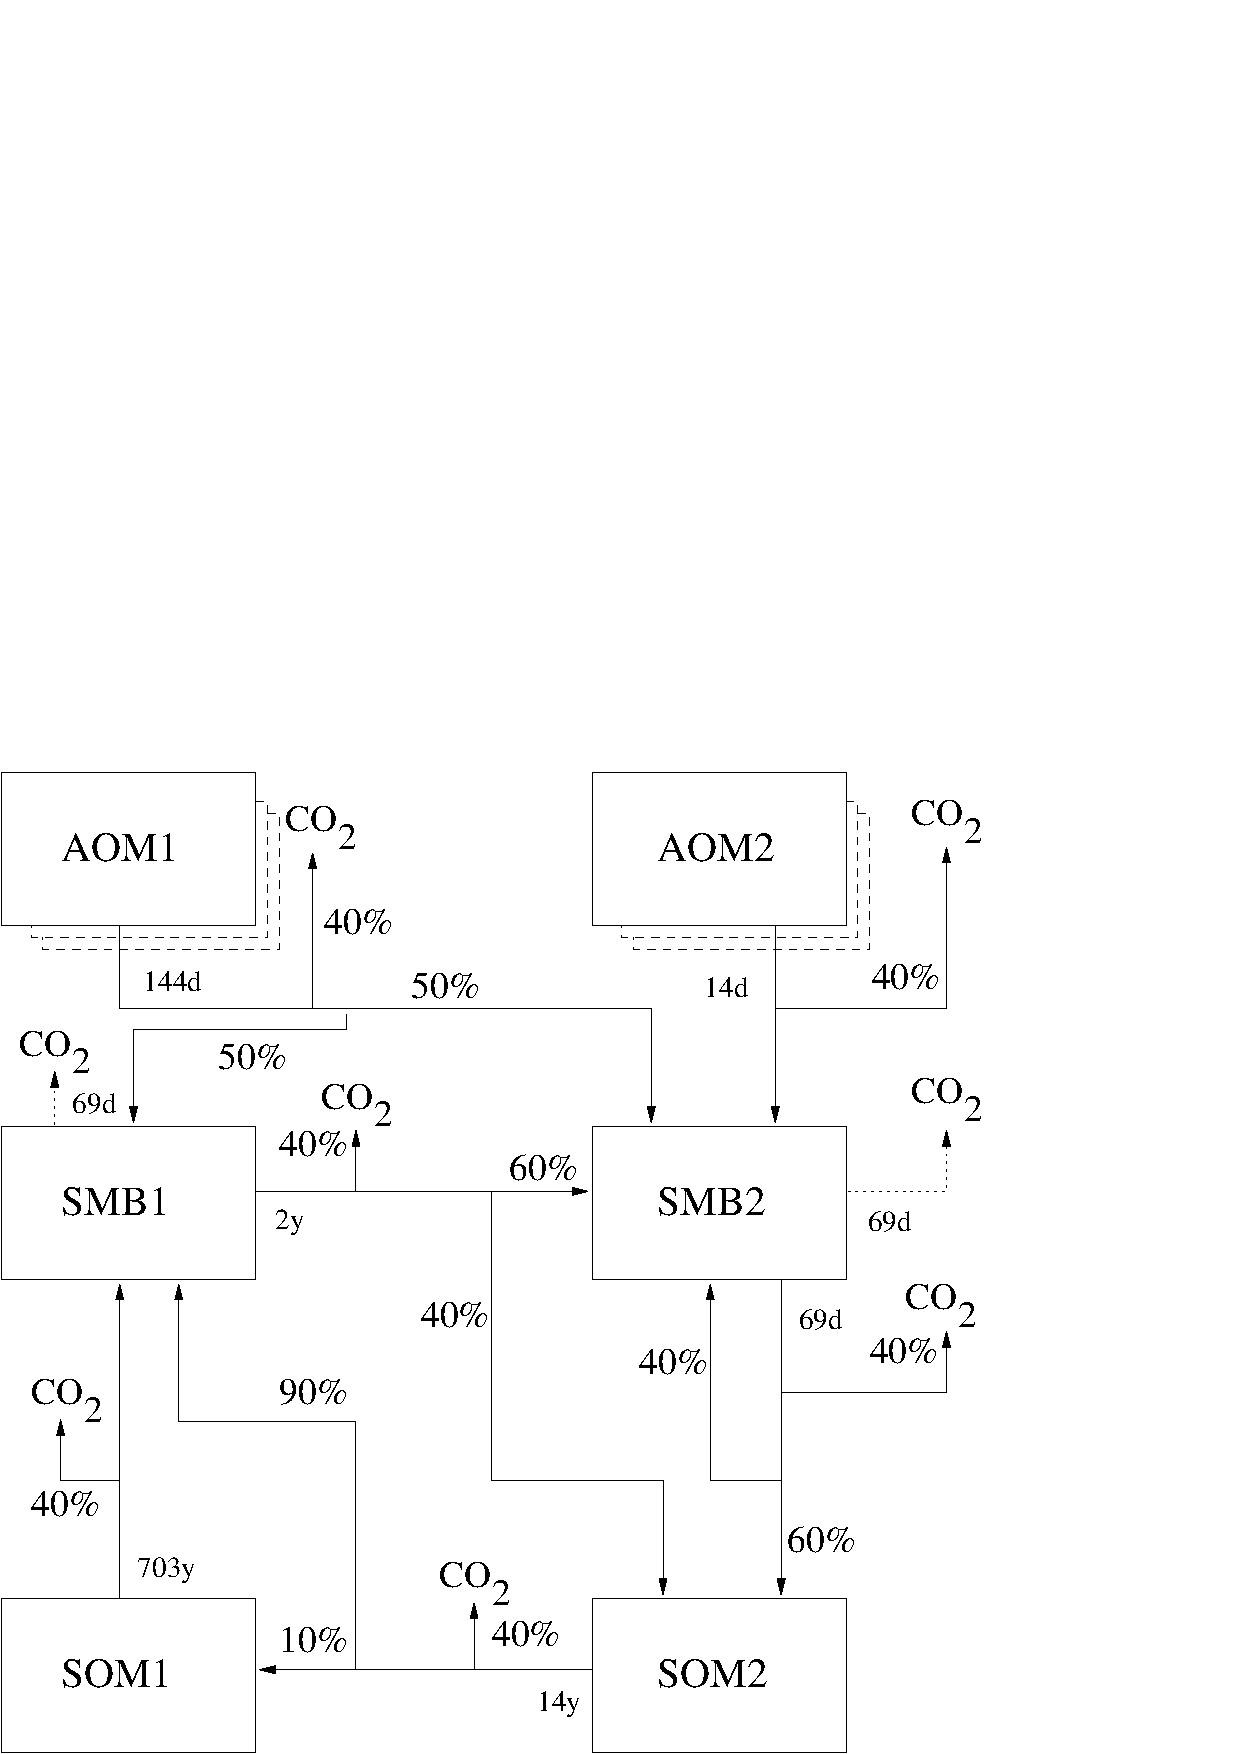
\includegraphics[width=0.8\hsize]{om1}

  \caption{The original \daisy{} OM parameterization.}
  \label{fig:om1}
\end{figure}

Figure~\ref{fig:om1} has 6 visible boxes, corresponding to the
\textsc{som}, \textsc{smb}, and \textsc{aom} pools, respectively.All
the pools have a fully drawn outgoing line. The amount of carbon
turned over and decomposed is directly proportional with the size of
the pool. We call this the \emph{turnover rate}. Looking at the
\textsc{som1} pool at the bottom left corner, it is noted that it has
one outgoing line, marked with the text ``703y''. This indicate the
turnover rate of this particular pool by the soil microbial biomass
and the number is the corresponding halftime. Thus, the \textsc{som1}
pool have a halftime of 703 years, meaning if there was no input it
would be half the original size after 703 years. For some pools this
time is given in days, e.g.\ the \textsc{smb2} pool has a turnover
halftime of 69 days.
  
If we follow the line from \textsc{som1} it splits into two parts.
40\% is lost in digestion as CO$_2$, the rest is allocated to the
microbial biomass in the \textsc{smb1} pool. Looking at the line going
out from the \textsc{som2} pool, we see that only 90\% of the carbon
not lost as CO$_2$ are allocated to the microbial biomass, the
remaining 10\% end up in \textsc{som1}. Besides a turnover rate, the
two pools of microbial biomasses have a maintenance rate. This rate
reflects the cost of staying alive, and is indicated by a stippled
line out of the \textsc{smb} pools. In general, the rates and even the
number of \textsc{aom} pools are variable, the rates given here are
just examples. Also, there can be many sets of added organic matter
pools, each set corresponds to a particular fertilizer or residual
with its specific parameters.

The coefficients of the turnover rate and maintenance of the pools is
affected by abiotic factors as clay conten in the soil, soil
temperature and moisture. The halftimes listed in figure~\ref{fig:om1}
corresponds to 0\% clay, 10$^\circ$C and field capacity (pF 2). The
halftimes will increase with increasing clay content, decreasing
temperature, or decreasing soil water content. Further information of
the abiotic factors included in the organic matter model in \daisy{}
is given in (XXXX).

\subsection{Evolution of the Daisy model}

The \daisy{} software allows the user to adjust the turnover rates,
the rate of maintenance, and directions of flow. It also allows the
user to specify the number of \textsc{som} and \textsc{smb} pools, as
well as the number of \textsc{aom} pools for each fertilizer
application and each crop residual type. Thus, the model provides a
good basis for experimentation.

The first such experimental change was made by M�ller
\citep{mueller-smb}, who adjusted the turnover rates of the
\textsc{smb} pools so the biomass content of the soil matched
the levels measured at the fields. The change did not affect the long
time dynamics of the system. The second change in parameterisation was
made by Bruun \citep{daisy-somnew}. This was a complete recalibration
that took into account the carbon input from rhizodepositions. This
change was more radical, involving both turnover rates and directions
of flow, and made the system much more adaptable to new levels of
input, another effect which has also been observed empirically
\citep{dk-humus-change}.

The current model is depicted in figure~\ref{fig:om2}. The purpose of
the \textsc{som3} pool in that figure will be explained later.

\begin{figure}[htbp]
  \centering
  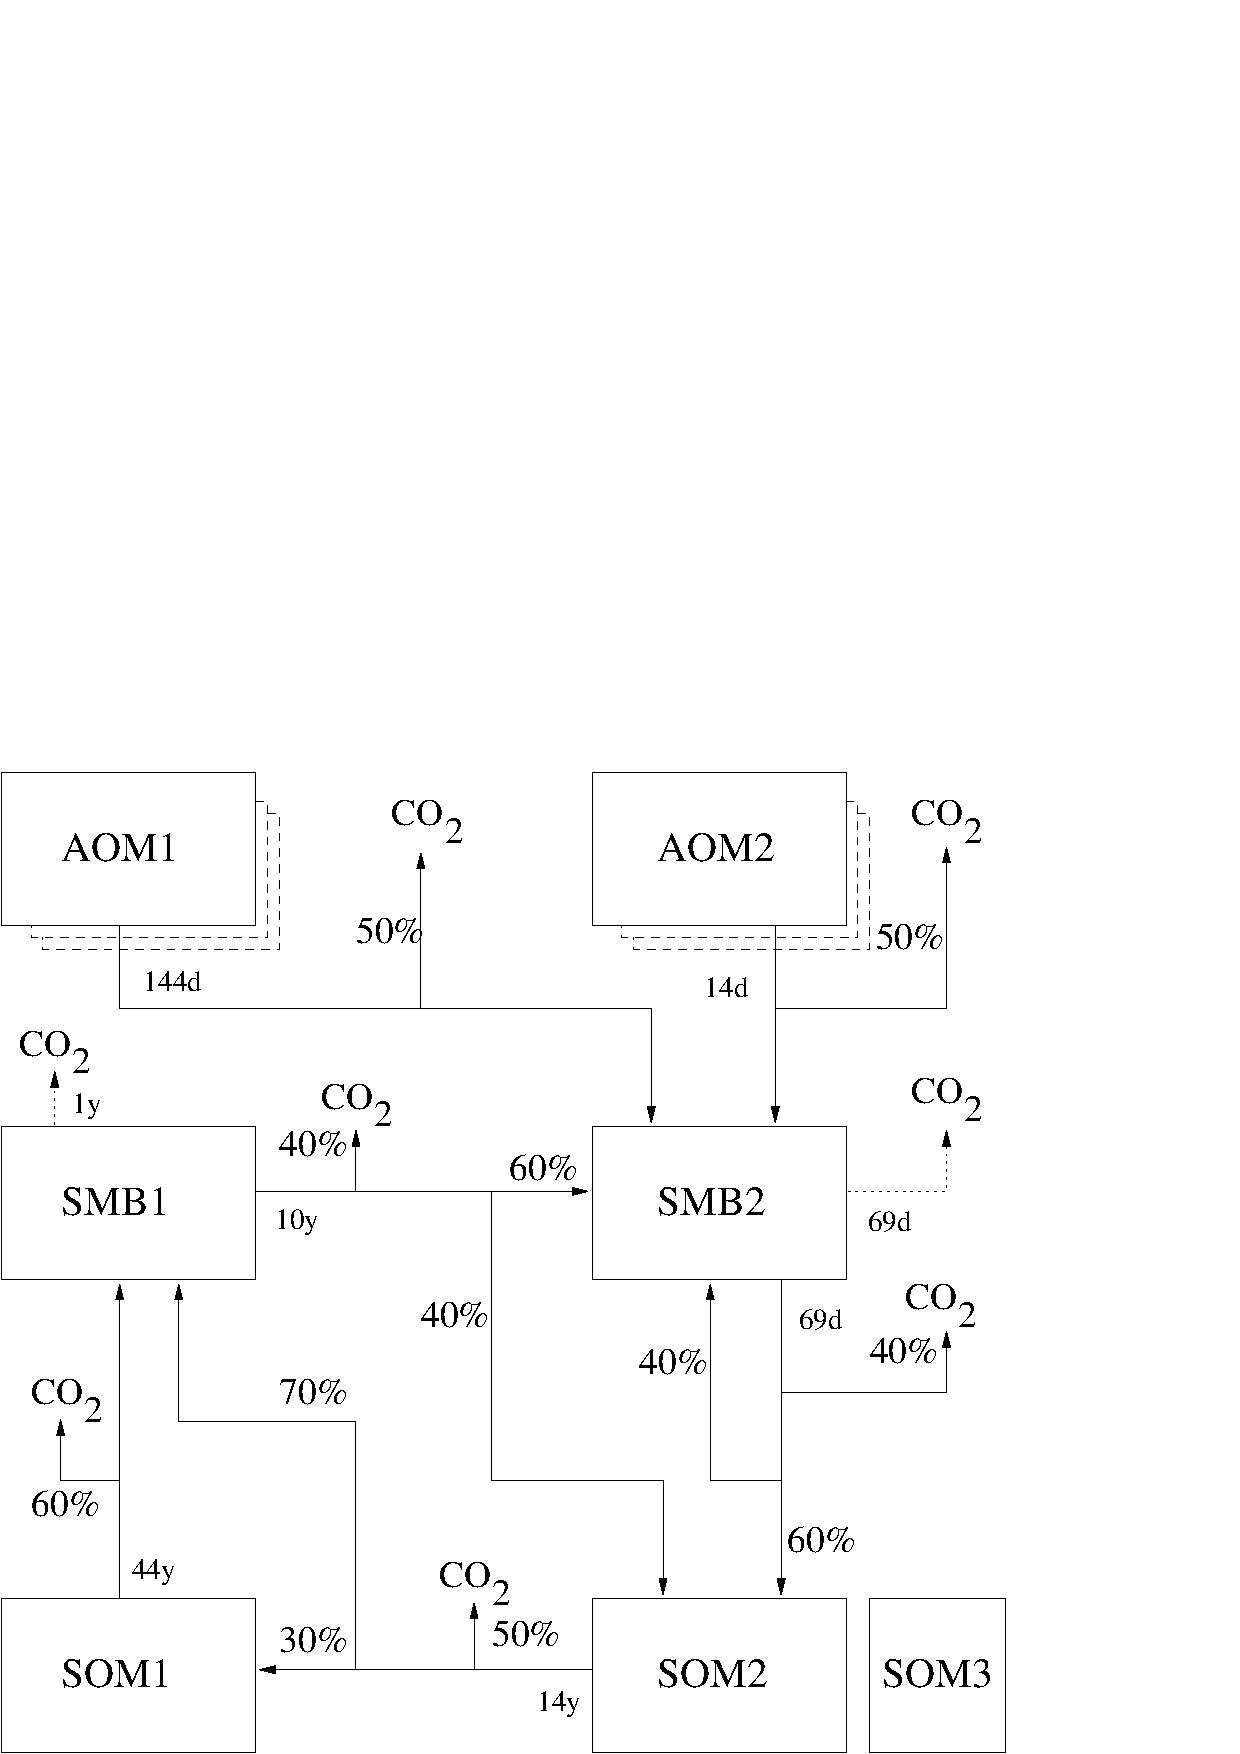
\includegraphics[width=0.8\hsize]{om2}
  
  \caption{New parameterization.}
  \label{fig:om2}
\end{figure}

Some of the experimental changes affecting soil organic matter that we
are currently working on, and which may be included in future versions
of \daisy{}, are dissolved organic matter \citep{bgj-dom}. Another
recalibration based on a larger experimental database and with special
focus on the effect of clay \citep{biomod,biomod2}, and a calibration
for forest soil (XXX). The conclusion is that the model has changed in
the past, and will continue to change in the future.

\subsection{Expanding user base}

The original development of \daisy{} was founded by the Danish
Environmental Protection Agency \citep{daisy-def}, and the first
non-research use was made by expert users who evaluated the national
environmental plans for limiting nitrogen contamination of groundwater
and surface water (see VMPuse).  Since then, \daisy{} has been used in
other parts of the environmental and agricultural agencies (see
\citep{novana} XXX), as well as increasingly by local authorities for
evaluating regional plans (see �rhus Amt og XXX), and recently also
for evaluation of applications for changed farm practice at an
individual farm level (see VVM, \citep{plantinfo-daisy}). For the last
case, \daisy{} has also been used by consulting agencies representing
``the other side'', namely farmers seeking permission to change
farming practice.

The effect of this increased use has been that we can no longer rely
on the users being experts. Therefore, a project was started in order
to provide standardized procedures for \daisy{} simulations (see XXX).
As part of this project, most components of \daisy{} was evaluated in
order to find parameters and submodels which could be initialized
automatically from default values, or from other parameters. These
parameters and submodels are still available to the expert user, but
are hidden for the user who do not have the expertise or data
available. The result is that the software now appears much simpler to
the user, even though no substantial changes to the model have been
made.

\subsection{Equilibrium assumptions}

Initialisation of the partition of the organic matter into the various
soil pools have been a particular stumbling block for most
users. Partly because it does not reflect an easily identifiable
property of the system being modelled. It is common to use an
equilibrium assumption for initializing models where measurements are
not available. For example, in \daisy{} we assume that the soil water
in the bottom of the unsaturated zone is in equilibrium with the
groundwater, as specified by Darcy's equation.  There are two
conditions where equilibrium is a good assumption: 1) when the system
quickly reach equilibrium compared to the external imposed changes, 2)
when the dynamic of the system quickly dominate over the initial
condition. The assumption of an initial equilibrium is good when a
reasonable initial state rather than a correct one is needed in the
model.

As part of the recalibration work conducted by Bruun
\citep{daisy-somnew}, they found that equilibrium between the
\textsc{som1} and \textsc{som2} was obtained very slowly up to XX
years for a XX system. They also found that the ratio between the
\textsc{som1} and \textsc{som2} for a system in equilibrium would be
49\% vs 51\%. Since \daisy{} after this recalibration required the
users to readjust the partitioning between \textsc{som1} and
\textsc{som2}, there was a strong tendency that users just picked the
equilibrium values.

Thus, the most used initialization condition of soil organic matter
pools, the equilibrium assumption, has been shown to be inaccurate in
many soil systems. As a consequence, a new initialisation method of
the soil organic matter pools is needed. The method should be robust
with regard to changes in the model or model parameterization, and at
the same time be expressible in terms of physical properties the user
can understand.


\subsection{Hypothesis}



\section{Methodology}
\subsection{Basic equations}

In order to find a better way to initialize the organic matter pools,
we will start by looking at the four equations describing their
internal relationships.
\begin{eqnarray}
  \Delta\mbox{\textsc{smb1}} &=& a\> \mbox{\textsc{smb1}} + b\>
  \mbox{\textsc{smb2}} + c\> \mbox{\textsc{som1}} + d\>
  \mbox{\textsc{som2}} + e\, \Delta\mbox{\textsc{aom}}\label{eq:dsmb1}\\
  \Delta\mbox{\textsc{smb2}} &=& f\> \mbox{\textsc{smb1}} + g\>
  \mbox{\textsc{smb2}} + h\> \mbox{\textsc{som1}} + i\>
  \mbox{\textsc{som2}} + j\, \Delta\mbox{\textsc{aom}}\\
  \Delta\mbox{\textsc{som1}} &=& k\> \mbox{\textsc{smb1}} + l\>
  \mbox{\textsc{smb2}} + m\> \mbox{\textsc{som1}} + n\>
  \mbox{\textsc{som2}} + o\, \Delta\mbox{\textsc{aom}}\\
  \Delta\mbox{\textsc{som2}} &=& p\> \mbox{\textsc{smb1}} + q\>
  \mbox{\textsc{smb2}} + r\> \mbox{\textsc{som1}} + s\>
  \mbox{\textsc{som2}} + t\, \Delta\mbox{\textsc{aom}}\label{eq:dsom2}
\end{eqnarray}
Here, we have excluded the \textsc{aom} pools, except as a source for
the other pools which we denote $\Delta\mbox{\textsc{aom}}$.
$\Delta\mbox{\textsc{aom}}$ is the total carbon input to the system.
The \textsc{aom} pools are special in that they are not feed by any of
the other pools, but by outside sources such as crop residuals and
fertilizer.  The other pools are described by content (\textsc{smb1},
\textsc{smb2}, \textsc{som1}, or \textsc{som2}) and change of content
($\Delta\mbox{\textsc{smb1}}$, $\Delta\mbox{\textsc{smb2}}$,
$\Delta\mbox{\textsc{som1}}$, $\Delta\mbox{\textsc{som2}}$).

The factors $a$ to $t$ depend on the model, so the factors are
different for the original model (figure~\ref{fig:om1}) and the Sander
recalibration (figure~\ref{fig:om2}).  They also depend on site and
time specific factors, namely the clay content of the soil, the
temperature, and the water potential.

Some of these factors may be zero, for example in none of the
calibrations mentioned we have any carbon going directly from the
\textsc{aom} pools to \textsc{som1}, so $o$ will always be zero.  We
include these anyway, because we are trying to solve the
initialization problem in a way that is robust with regard to changes
in the model.  The description is also robust with regard to the
number of pools\footnote{The generalized form used by the \daisy{}
  program is:
  \begin{equation}
    \begin{array}{rclcr}
      \Delta\mbox{\textsc{smb}}i &=& \displaystyle
      \sum_{k=1}^{\mbox{\tiny\#\textsc{smb}}} a_{i,k}\,\mbox{\textsc{smb}}k + 
      \sum_{l=1}^{\mbox{\tiny\#\textsc{som}}} b_{i,l}\,\mbox{\textsc{som}}l +
      c_i \Delta\mbox{\textsc{aom}} 
      &;&i = 1\ldots\mbox{\#\textsc{smb}}\nonumber\\
      \Delta\mbox{\textsc{som}}j &=& \displaystyle
      \sum_{k=1}^{\mbox{\tiny\#\textsc{smb}}} d_{j,k}\,\mbox{\textsc{smb}}k +
      \sum_{l=1}^{\mbox{\tiny\#\textsc{som}}} e_{j,l}\,\mbox{\textsc{som}}l +
      f_j \Delta\mbox{\textsc{aom}} 
      &;&j = 1\ldots\mbox{\#\textsc{som}}\nonumber
    \end{array}
  \end{equation}
}, adding a new pool will add one more equation, and two new unknowns.

Back to the two pool example.  We have four equations and nine
unknowns.  We need more information.  The first piece of information
we can add is the total organic matter content in the field, which can
be directly measured.  This gives us one new equation, and two new
variables.
\begin{equation}
  \label{eq:total}
  \mbox{\textsc{total}} = \mbox{\textsc{smb1}} + \mbox{\textsc{smb2}}
  + \mbox{\textsc{som1}} + \mbox{\textsc{som2}} + \mbox{\textsc{aom}}
\end{equation}
\textsc{total} is measured. \mbox{\textsc{aom}}, the initial content
of added organic matter, is given a default value corresponding to
typical root residuals left from a crop.  We now need four more
equations\footnote{Everybody: Four more equations!  Four more
  equations!}, one for each pool.

\section{Quasi-equilibrium}

The equilibrium assumption corresponds to adding these four equations: 
\begin{equation}
  \Delta\mbox{\textsc{smb1}} = \Delta\mbox{\textsc{smb2}} 
  = \Delta\mbox{\textsc{som1}} = \Delta\mbox{\textsc{som2}} = 0
\end{equation}
Even though we earlier argued that it was not good for initializing
the system, we can use it to obtain an estimate of
$\Delta\mbox{\textsc{aom}}$, the carbon input level required to
maintain the measured amount of organic matter in the soil, which may
be interesting in itself, for example in a discussion about soil
quality or global change.

The initializing procedure we ended up using was to allows the slowest
pool (which happens to be \textsc{som1}) to change, but requires the
user to specify the carbon input to the system ($u$).  We then get:
\begin{eqnarray}
  \Delta\mbox{\textsc{smb1}} &=& 0\\
  \Delta\mbox{\textsc{smb2}} &=& 0\\
  \Delta\mbox{\textsc{som2}} &=& 0\label{eq:fastpooleq}\\
  \Delta\mbox{\textsc{aom}} &=& u
\end{eqnarray}

We now have nine equations with nine unknowns, and can initialize the
system.  The physical interpretation of this initialization is that
all but the slowest pool have reached a quasi-equilibrium with respect
to the input, and the size of the slowest pool.  Since the slowest
pool is still changing (and the other pools will have to change to
reflect that), this is not a true equilibrium.
Figure~\ref{fig:clayom} and~\ref{fig:sandom} shows that the fast
\textsc{som} pool (\textsc{som2}) does indeed adapt to changes in
input much faster than the slow pool (\textsc{som1}), the hump in each
graph is due to that effect.

\subsection{User calibration}

We also have a model independent knob for users who want to calibrate
the system.  If the user can estimate the total rate of change in
carbon content, i.e.\ is the soil gaining or losing organic matter
with the specified input, we can substitute
equation~\ref{eq:fastpooleq} with
\begin{equation}
  \Delta\mbox{\textsc{smb1}} + \Delta\mbox{\textsc{smb2}} 
  + \Delta\mbox{\textsc{som1}} + \Delta\mbox{\textsc{som2}} = v
\end{equation}
where $v$ is the user specified change in carbon content.  Since our
users are generally more concerned with nitrogen than with carbon, we
ask them to specify the \emph{background mineralization} ($w$), which
is the amount of nitrogen the rest of the system gets or loses from
the soil.  The equation is then
\begin{equation}
  \frac{\Delta\mbox{\textsc{smb1}}}{{C/N}_{\mbox{\small\textsc {smb1}}}}
  + \frac{\Delta\mbox{\textsc{smb2}}}{{C/N}_{\mbox{\small\textsc{smb2}}}}
  + \frac{\Delta\mbox{\textsc{som1}}}{{C/N}_{\mbox{\small\textsc{som1}}}}
  + \frac{\Delta\mbox{\textsc{som2}}}{{C/N}_{\mbox{\small\textsc{som2}}}}
  = w
\end{equation}
Note that the simulated background mineralization will only be the
specified value ($w$) if the simulated carbon input also corresponds
to the specified value ($u$).  If we are simulating the effect of a
proposed change in management practice, this will not be the
case. Another caveat is that \daisy{} treat the $C/N$ for matter
entering the \textsc{som} pools independently of the $C/N$ leaving
them. The equation will only be correct when the two are close.

In conclusion, we can now initialize the soil organic matter system
from two or three numbers supplied by the user.  The two mandatory
numbers are the total content of organic matter, and an estimate of
how much carbon has been added to the system per year in the recent
decades.  The third, optional, number is the estimated background
mineralization.  The first number is directly measurable, the two
other can at least be understood by people who have no intimate
knowledge of the model, and can be estimated by the user, for example
from the use of \daisy{} simulations.  None of the these numbers need
to be changed when the model itself is changed.

\subsection{Abiotic factors}

In the equations~\ref{eq:dsmb1} to~\ref{eq:dsom2} we used a large number
of constants, without indicating how we calculate them.  Here is the
formula for calculating $a$ from the first equation.
\begin{displaymath}
  a = (t_{\mbox{\tiny\textsc{smb1}}}\,
  (X_{\mbox{\tiny\textsc{smb1}}\rightarrow{\mbox{\tiny\textsc{smb1}}}}\,
  E_{\mbox{\tiny\textsc{smb1}}}
  - 1) - m_{\mbox{\tiny\textsc{smb1}}})\,
  F_{\mbox{\tiny\textsc{smb1}}}^T (T)\,
  F_{\mbox{\tiny\textsc{smb1}}}^\psi (\psi)\,
  F_{\mbox{\tiny\textsc{smb1}}}^C (X_c)
\end{displaymath}
The other constants have a similar form.
$t_{\mbox{\tiny\textsc{smb1}}}$ is the turnover rate for the
\textsc{smb1} pool.
$X_{\mbox{\tiny\textsc{smb1}}\rightarrow{\mbox{\tiny\textsc{smb1}}}}$
is the carbon fraction going from \textsc{smb1} back to \textsc{smb1}.
$E_{\mbox{\tiny\textsc{smb1}}}$ is the efficiency of which
\textsc{smb1} can be digested, the remaining part will be lost as
CO$_2$.  $m_{\mbox{\tiny\textsc{smb1}}}$ is the maintenance cost of
the \textsc{smb1} pool. $F_{\mbox{\tiny\textsc{smb1}}}^T$,
$F_{\mbox{\tiny\textsc{smb1}}}^\psi$, and
$F_{\mbox{\tiny\textsc{smb1}}}^C$ are the abiotic factors for soil
heat, moisture and clay respectively.  All of these are part of the
basic model calibration, and unchanged for all normal use of the model.

What does change is the soil temperature ($T$), soil moisture
($\psi$), and clay content ($X_c$).  The clay content is constant
during the time-scales we work on, and is specified by the user.  So
the two problematic terms are $T$ and $\psi$ which are variable during
the simulation.  For the initialization we must use constant values.
By default we use the average temperature for the site (which is
already specified by the user and used elsewhere in the model) for
$T$, and field capacity (pF 2) for $\psi$.  As $F^T$ is non-linear,
using the average is incorrect.  In particular, $F^T$ is zero for $T <
0^\circ$C, so for a cold climate like the Danish the significance of
frost is overestimated.  On the other hand, using pF 2 may be
acceptable for the wet climate like in Denmark, but may be
unreasonable for a dry climate.  The two factors interact, so a low
value for $F^T (T)$ is most significant when $F^\psi (\psi)$ is high,
and vice-versa.  So in effect we can treat $T$ and $\psi$ as
calibration parameters when using \daisy{} in a different climate.  By
logging the product of factors in a realistic simulation, \daisy{} can
be used to calculate the combined effect.  From that, the user can
choose values for $T$ and $\psi$ that give the same effect.

\subsection{Inert organic matter}

The current \daisy{} model calibration is based primarily on
measurements on agricultural topsoil \citep{daisy-somnew,mueller-smb},
where all the humus is presumed to be active.  This means the
calibration is not good for subsoils, nor for some types of humus-rich
topsoils.  The \textsc{som3} pool you last saw in figure~\ref{fig:om2}
exists to compensate for these shortcomings.  The \textsc{som3} pool
is inert, so for the soil organic matter system it is as if the humus
in the pool didn't exist.  The inert humus still affects other aspects
of \daisy{}, such as the hydraulic and adsorption properties of the
soil.

For the subsoil, we by default assume the system is in equilibrium
with the input, and park enough humus in the \textsc{som3} pool so
that this assumption holds true.  The observant reader will remember
that we earlier argued that the equilibrium assumption is wrong.  It
still is, also for the subsoil.  However, the subsoil contribute
relatively little to the total system (XXX), so we can get away with
this assumption.  For topsoil, the user can explicitly park some of
the humus in the \textsc{som3} pool, if he has reason to believe it to
be necessary.

\section{Results and Discussion}
\subsection{Comparisons}

PA: Diskution af fig3 og 4 quasi-eq

PA: Overvej initialisering med ``background mineralization = 0''.

PA: Ref til \citep{daisy-init}.



\subsection{Long term simulations}
NOTER As part of the standardization project mentioned earlier,
\daisy{} was used to simulate the effect of changing farming practice
on soil organic matter.  Figure~\ref{fig:clayom} shows humus content
for a system that goes from equilibrium at a high level of carbon
input, to equilibrium at a low level of carbon input. Danish farming
practice has been used, as well as Danish climate and soil. The soil
has a for Danish conditions a relative high clay content (12\%).
Figure~\ref{fig:clayom} also shows the simulated \textsc{som1}
fraction of total \textsc{som}. Finally, figure~\ref{fig:sandom} shows
that a simulation on a COARSE SANDY SOIL going from a low to high
input equilibrium.

\begin{figure}[htbp]
  \centering
  % GNUPLOT: LaTeX picture
\setlength{\unitlength}{0.240900pt}
\ifx\plotpoint\undefined\newsavebox{\plotpoint}\fi
\begin{picture}(1500,900)(0,0)
\sbox{\plotpoint}{\rule[-0.200pt]{0.400pt}{0.400pt}}%
\put(140,123){\makebox(0,0)[r]{$0$}}
\put(160.0,123.0){\rule[-0.200pt]{4.818pt}{0.400pt}}
\put(140,254){\makebox(0,0)[r]{$0.5$}}
\put(160.0,254.0){\rule[-0.200pt]{4.818pt}{0.400pt}}
\put(140,385){\makebox(0,0)[r]{$1$}}
\put(160.0,385.0){\rule[-0.200pt]{4.818pt}{0.400pt}}
\put(140,515){\makebox(0,0)[r]{$1.5$}}
\put(160.0,515.0){\rule[-0.200pt]{4.818pt}{0.400pt}}
\put(140,646){\makebox(0,0)[r]{$2$}}
\put(160.0,646.0){\rule[-0.200pt]{4.818pt}{0.400pt}}
\put(140,777){\makebox(0,0)[r]{$2.5$}}
\put(160.0,777.0){\rule[-0.200pt]{4.818pt}{0.400pt}}
\put(160,82){\makebox(0,0){$2000$}}
\put(160.0,123.0){\rule[-0.200pt]{0.400pt}{4.818pt}}
\put(180.0,123.0){\rule[-0.200pt]{0.400pt}{2.409pt}}
\put(200.0,123.0){\rule[-0.200pt]{0.400pt}{2.409pt}}
\put(221.0,123.0){\rule[-0.200pt]{0.400pt}{2.409pt}}
\put(241.0,123.0){\rule[-0.200pt]{0.400pt}{2.409pt}}
\put(261.0,123.0){\rule[-0.200pt]{0.400pt}{2.409pt}}
\put(282.0,123.0){\rule[-0.200pt]{0.400pt}{2.409pt}}
\put(302.0,123.0){\rule[-0.200pt]{0.400pt}{2.409pt}}
\put(322.0,123.0){\rule[-0.200pt]{0.400pt}{2.409pt}}
\put(363,82){\makebox(0,0){$2100$}}
\put(363.0,123.0){\rule[-0.200pt]{0.400pt}{4.818pt}}
\put(383.0,123.0){\rule[-0.200pt]{0.400pt}{2.409pt}}
\put(403.0,123.0){\rule[-0.200pt]{0.400pt}{2.409pt}}
\put(424.0,123.0){\rule[-0.200pt]{0.400pt}{2.409pt}}
\put(444.0,123.0){\rule[-0.200pt]{0.400pt}{2.409pt}}
\put(464.0,123.0){\rule[-0.200pt]{0.400pt}{2.409pt}}
\put(484.0,123.0){\rule[-0.200pt]{0.400pt}{2.409pt}}
\put(505.0,123.0){\rule[-0.200pt]{0.400pt}{2.409pt}}
\put(525.0,123.0){\rule[-0.200pt]{0.400pt}{2.409pt}}
\put(566,82){\makebox(0,0){$2200$}}
\put(566.0,123.0){\rule[-0.200pt]{0.400pt}{4.818pt}}
\put(586.0,123.0){\rule[-0.200pt]{0.400pt}{2.409pt}}
\put(606.0,123.0){\rule[-0.200pt]{0.400pt}{2.409pt}}
\put(626.0,123.0){\rule[-0.200pt]{0.400pt}{2.409pt}}
\put(647.0,123.0){\rule[-0.200pt]{0.400pt}{2.409pt}}
\put(667.0,123.0){\rule[-0.200pt]{0.400pt}{2.409pt}}
\put(687.0,123.0){\rule[-0.200pt]{0.400pt}{2.409pt}}
\put(708.0,123.0){\rule[-0.200pt]{0.400pt}{2.409pt}}
\put(728.0,123.0){\rule[-0.200pt]{0.400pt}{2.409pt}}
\put(768,82){\makebox(0,0){$2300$}}
\put(768.0,123.0){\rule[-0.200pt]{0.400pt}{4.818pt}}
\put(789.0,123.0){\rule[-0.200pt]{0.400pt}{2.409pt}}
\put(809.0,123.0){\rule[-0.200pt]{0.400pt}{2.409pt}}
\put(829.0,123.0){\rule[-0.200pt]{0.400pt}{2.409pt}}
\put(850.0,123.0){\rule[-0.200pt]{0.400pt}{2.409pt}}
\put(870.0,123.0){\rule[-0.200pt]{0.400pt}{2.409pt}}
\put(890.0,123.0){\rule[-0.200pt]{0.400pt}{2.409pt}}
\put(910.0,123.0){\rule[-0.200pt]{0.400pt}{2.409pt}}
\put(931.0,123.0){\rule[-0.200pt]{0.400pt}{2.409pt}}
\put(971,82){\makebox(0,0){$2400$}}
\put(971.0,123.0){\rule[-0.200pt]{0.400pt}{4.818pt}}
\put(992.0,123.0){\rule[-0.200pt]{0.400pt}{2.409pt}}
\put(1012.0,123.0){\rule[-0.200pt]{0.400pt}{2.409pt}}
\put(1032.0,123.0){\rule[-0.200pt]{0.400pt}{2.409pt}}
\put(1052.0,123.0){\rule[-0.200pt]{0.400pt}{2.409pt}}
\put(1073.0,123.0){\rule[-0.200pt]{0.400pt}{2.409pt}}
\put(1093.0,123.0){\rule[-0.200pt]{0.400pt}{2.409pt}}
\put(1113.0,123.0){\rule[-0.200pt]{0.400pt}{2.409pt}}
\put(1134.0,123.0){\rule[-0.200pt]{0.400pt}{2.409pt}}
\put(1174,82){\makebox(0,0){$2500$}}
\put(1174.0,123.0){\rule[-0.200pt]{0.400pt}{4.818pt}}
\put(1194.0,123.0){\rule[-0.200pt]{0.400pt}{2.409pt}}
\put(1215.0,123.0){\rule[-0.200pt]{0.400pt}{2.409pt}}
\put(1235.0,123.0){\rule[-0.200pt]{0.400pt}{2.409pt}}
\put(1255.0,123.0){\rule[-0.200pt]{0.400pt}{2.409pt}}
\put(1276.0,123.0){\rule[-0.200pt]{0.400pt}{2.409pt}}
\put(1296.0,123.0){\rule[-0.200pt]{0.400pt}{2.409pt}}
\put(1316.0,123.0){\rule[-0.200pt]{0.400pt}{2.409pt}}
\put(1336.0,123.0){\rule[-0.200pt]{0.400pt}{2.409pt}}
\put(1377,82){\makebox(0,0){$2600$}}
\put(1377.0,123.0){\rule[-0.200pt]{0.400pt}{4.818pt}}
\put(1399,197){\makebox(0,0)[l]{ 30}}
\put(1359.0,197.0){\rule[-0.200pt]{4.818pt}{0.400pt}}
\put(1399,344){\makebox(0,0)[l]{ 40}}
\put(1359.0,344.0){\rule[-0.200pt]{4.818pt}{0.400pt}}
\put(1399,492){\makebox(0,0)[l]{ 50}}
\put(1359.0,492.0){\rule[-0.200pt]{4.818pt}{0.400pt}}
\put(1399,639){\makebox(0,0)[l]{ 60}}
\put(1359.0,639.0){\rule[-0.200pt]{4.818pt}{0.400pt}}
\put(1399,786){\makebox(0,0)[l]{ 70}}
\put(1359.0,786.0){\rule[-0.200pt]{4.818pt}{0.400pt}}
\put(160.0,123.0){\rule[-0.200pt]{293.657pt}{0.400pt}}
\put(1379.0,123.0){\rule[-0.200pt]{0.400pt}{177.543pt}}
\put(160.0,123.0){\rule[-0.200pt]{0.400pt}{177.543pt}}
\put(769,21){\makebox(0,0){Year}}
\put(972,823){\makebox(0,0)[l]{humus [\%]}}
\put(852.0,823.0){\rule[-0.200pt]{24.090pt}{0.400pt}}
\put(261,850){\usebox{\plotpoint}}
\put(260.67,848){\rule{0.400pt}{0.482pt}}
\multiput(260.17,849.00)(1.000,-1.000){2}{\rule{0.400pt}{0.241pt}}
\put(262.0,842.0){\rule[-0.200pt]{0.400pt}{1.445pt}}
\put(262.0,842.0){\usebox{\plotpoint}}
\put(262.0,843.0){\usebox{\plotpoint}}
\put(263.0,843.0){\rule[-0.200pt]{0.400pt}{3.613pt}}
\put(263,845.67){\rule{0.241pt}{0.400pt}}
\multiput(263.00,846.17)(0.500,-1.000){2}{\rule{0.120pt}{0.400pt}}
\put(263.0,847.0){\rule[-0.200pt]{0.400pt}{2.650pt}}
\put(264,846){\usebox{\plotpoint}}
\put(263.67,832){\rule{0.400pt}{0.723pt}}
\multiput(263.17,833.50)(1.000,-1.500){2}{\rule{0.400pt}{0.361pt}}
\put(264.0,835.0){\rule[-0.200pt]{0.400pt}{2.650pt}}
\put(265,823.67){\rule{0.241pt}{0.400pt}}
\multiput(265.00,824.17)(0.500,-1.000){2}{\rule{0.120pt}{0.400pt}}
\put(265.0,825.0){\rule[-0.200pt]{0.400pt}{1.686pt}}
\put(266.0,824.0){\rule[-0.200pt]{0.400pt}{8.672pt}}
\put(266,841.67){\rule{0.241pt}{0.400pt}}
\multiput(266.00,842.17)(0.500,-1.000){2}{\rule{0.120pt}{0.400pt}}
\put(266.0,843.0){\rule[-0.200pt]{0.400pt}{4.095pt}}
\put(267,829.67){\rule{0.241pt}{0.400pt}}
\multiput(267.00,830.17)(0.500,-1.000){2}{\rule{0.120pt}{0.400pt}}
\put(267.0,831.0){\rule[-0.200pt]{0.400pt}{2.650pt}}
\put(268.0,827.0){\rule[-0.200pt]{0.400pt}{0.723pt}}
\put(268.0,827.0){\usebox{\plotpoint}}
\put(268.0,828.0){\usebox{\plotpoint}}
\put(269,819.67){\rule{0.241pt}{0.400pt}}
\multiput(269.00,820.17)(0.500,-1.000){2}{\rule{0.120pt}{0.400pt}}
\put(269.0,821.0){\rule[-0.200pt]{0.400pt}{1.686pt}}
\put(270,820){\usebox{\plotpoint}}
\put(270,820){\usebox{\plotpoint}}
\put(270.0,818.0){\rule[-0.200pt]{0.400pt}{0.482pt}}
\put(270.0,818.0){\usebox{\plotpoint}}
\put(271.0,818.0){\rule[-0.200pt]{0.400pt}{3.854pt}}
\put(271,824.67){\rule{0.241pt}{0.400pt}}
\multiput(271.00,825.17)(0.500,-1.000){2}{\rule{0.120pt}{0.400pt}}
\put(271.0,826.0){\rule[-0.200pt]{0.400pt}{1.927pt}}
\put(272,825){\usebox{\plotpoint}}
\put(271.67,815){\rule{0.400pt}{0.723pt}}
\multiput(271.17,816.50)(1.000,-1.500){2}{\rule{0.400pt}{0.361pt}}
\put(272.0,818.0){\rule[-0.200pt]{0.400pt}{1.686pt}}
\put(273.0,814.0){\usebox{\plotpoint}}
\put(273.0,814.0){\rule[-0.200pt]{0.400pt}{0.723pt}}
\put(273.0,812.0){\rule[-0.200pt]{0.400pt}{1.204pt}}
\put(273.0,812.0){\usebox{\plotpoint}}
\put(274.0,809.0){\rule[-0.200pt]{0.400pt}{0.723pt}}
\put(274.0,809.0){\usebox{\plotpoint}}
\put(275.0,809.0){\rule[-0.200pt]{0.400pt}{1.445pt}}
\put(275.0,810.0){\rule[-0.200pt]{0.400pt}{1.204pt}}
\put(275.0,810.0){\usebox{\plotpoint}}
\put(276,805.67){\rule{0.241pt}{0.400pt}}
\multiput(276.00,805.17)(0.500,1.000){2}{\rule{0.120pt}{0.400pt}}
\put(276.0,806.0){\rule[-0.200pt]{0.400pt}{0.964pt}}
\put(277.0,807.0){\rule[-0.200pt]{0.400pt}{3.373pt}}
\put(277,812.67){\rule{0.241pt}{0.400pt}}
\multiput(277.00,813.17)(0.500,-1.000){2}{\rule{0.120pt}{0.400pt}}
\put(277.0,814.0){\rule[-0.200pt]{0.400pt}{1.686pt}}
\put(278,805.67){\rule{0.241pt}{0.400pt}}
\multiput(278.00,806.17)(0.500,-1.000){2}{\rule{0.120pt}{0.400pt}}
\put(278.0,807.0){\rule[-0.200pt]{0.400pt}{1.445pt}}
\put(279.0,806.0){\rule[-0.200pt]{0.400pt}{3.854pt}}
\put(279,813.67){\rule{0.241pt}{0.400pt}}
\multiput(279.00,814.17)(0.500,-1.000){2}{\rule{0.120pt}{0.400pt}}
\put(279.0,815.0){\rule[-0.200pt]{0.400pt}{1.686pt}}
\put(279.67,805){\rule{0.400pt}{0.723pt}}
\multiput(279.17,806.50)(1.000,-1.500){2}{\rule{0.400pt}{0.361pt}}
\put(280.0,808.0){\rule[-0.200pt]{0.400pt}{1.445pt}}
\put(281,792.67){\rule{0.241pt}{0.400pt}}
\multiput(281.00,793.17)(0.500,-1.000){2}{\rule{0.120pt}{0.400pt}}
\put(281.0,794.0){\rule[-0.200pt]{0.400pt}{2.650pt}}
\put(282,793){\usebox{\plotpoint}}
\put(282.0,792.0){\usebox{\plotpoint}}
\put(282.0,792.0){\rule[-0.200pt]{0.400pt}{7.709pt}}
\put(281.67,811){\rule{0.400pt}{1.204pt}}
\multiput(281.17,813.50)(1.000,-2.500){2}{\rule{0.400pt}{0.602pt}}
\put(282.0,816.0){\rule[-0.200pt]{0.400pt}{1.927pt}}
\put(282.67,797){\rule{0.400pt}{0.482pt}}
\multiput(282.17,798.00)(1.000,-1.000){2}{\rule{0.400pt}{0.241pt}}
\put(283.0,799.0){\rule[-0.200pt]{0.400pt}{2.891pt}}
\put(284,797){\usebox{\plotpoint}}
\put(284,797){\usebox{\plotpoint}}
\put(284,797){\usebox{\plotpoint}}
\put(284.0,795.0){\rule[-0.200pt]{0.400pt}{0.482pt}}
\put(284.0,795.0){\usebox{\plotpoint}}
\put(285.0,795.0){\rule[-0.200pt]{0.400pt}{0.482pt}}
\put(285,787.67){\rule{0.241pt}{0.400pt}}
\multiput(285.00,788.17)(0.500,-1.000){2}{\rule{0.120pt}{0.400pt}}
\put(285.0,789.0){\rule[-0.200pt]{0.400pt}{1.927pt}}
\put(285.67,785){\rule{0.400pt}{0.482pt}}
\multiput(285.17,785.00)(1.000,1.000){2}{\rule{0.400pt}{0.241pt}}
\put(286.0,785.0){\rule[-0.200pt]{0.400pt}{0.723pt}}
\put(287.0,787.0){\rule[-0.200pt]{0.400pt}{5.059pt}}
\put(286.67,799){\rule{0.400pt}{0.482pt}}
\multiput(286.17,800.00)(1.000,-1.000){2}{\rule{0.400pt}{0.241pt}}
\put(287.0,801.0){\rule[-0.200pt]{0.400pt}{1.686pt}}
\put(287.67,790){\rule{0.400pt}{0.723pt}}
\multiput(287.17,791.50)(1.000,-1.500){2}{\rule{0.400pt}{0.361pt}}
\put(288.0,793.0){\rule[-0.200pt]{0.400pt}{1.445pt}}
\put(289.0,783.0){\rule[-0.200pt]{0.400pt}{1.686pt}}
\put(289.0,783.0){\rule[-0.200pt]{0.400pt}{0.964pt}}
\put(289,782.67){\rule{0.241pt}{0.400pt}}
\multiput(289.00,783.17)(0.500,-1.000){2}{\rule{0.120pt}{0.400pt}}
\put(289.0,784.0){\rule[-0.200pt]{0.400pt}{0.723pt}}
\put(290,777.67){\rule{0.241pt}{0.400pt}}
\multiput(290.00,778.17)(0.500,-1.000){2}{\rule{0.120pt}{0.400pt}}
\put(290.0,779.0){\rule[-0.200pt]{0.400pt}{0.964pt}}
\put(291.0,777.0){\usebox{\plotpoint}}
\put(291.0,777.0){\rule[-0.200pt]{0.400pt}{0.482pt}}
\put(291,773.67){\rule{0.241pt}{0.400pt}}
\multiput(291.00,774.17)(0.500,-1.000){2}{\rule{0.120pt}{0.400pt}}
\put(291.0,775.0){\rule[-0.200pt]{0.400pt}{0.964pt}}
\put(292.0,771.0){\rule[-0.200pt]{0.400pt}{0.723pt}}
\put(292.0,771.0){\usebox{\plotpoint}}
\put(293.0,771.0){\rule[-0.200pt]{0.400pt}{3.132pt}}
\put(293,779.67){\rule{0.241pt}{0.400pt}}
\multiput(293.00,780.17)(0.500,-1.000){2}{\rule{0.120pt}{0.400pt}}
\put(293.0,781.0){\rule[-0.200pt]{0.400pt}{0.723pt}}
\put(294,774.67){\rule{0.241pt}{0.400pt}}
\multiput(294.00,775.17)(0.500,-1.000){2}{\rule{0.120pt}{0.400pt}}
\put(294.0,776.0){\rule[-0.200pt]{0.400pt}{0.964pt}}
\put(295.0,774.0){\usebox{\plotpoint}}
\put(295.0,774.0){\rule[-0.200pt]{0.400pt}{3.613pt}}
\put(294.67,782){\rule{0.400pt}{0.723pt}}
\multiput(294.17,783.50)(1.000,-1.500){2}{\rule{0.400pt}{0.361pt}}
\put(295.0,785.0){\rule[-0.200pt]{0.400pt}{0.964pt}}
\put(295.67,774){\rule{0.400pt}{0.482pt}}
\multiput(295.17,775.00)(1.000,-1.000){2}{\rule{0.400pt}{0.241pt}}
\put(296.0,776.0){\rule[-0.200pt]{0.400pt}{1.445pt}}
\put(297,762.67){\rule{0.241pt}{0.400pt}}
\multiput(297.00,763.17)(0.500,-1.000){2}{\rule{0.120pt}{0.400pt}}
\put(297.0,764.0){\rule[-0.200pt]{0.400pt}{2.409pt}}
\put(298,763){\usebox{\plotpoint}}
\put(298,763){\usebox{\plotpoint}}
\put(298,763){\usebox{\plotpoint}}
\put(297.67,788){\rule{0.400pt}{1.445pt}}
\multiput(297.17,791.00)(1.000,-3.000){2}{\rule{0.400pt}{0.723pt}}
\put(298.0,763.0){\rule[-0.200pt]{0.400pt}{7.468pt}}
\put(299.0,777.0){\rule[-0.200pt]{0.400pt}{2.650pt}}
\put(299.0,777.0){\rule[-0.200pt]{0.400pt}{0.964pt}}
\put(298.67,775){\rule{0.400pt}{0.723pt}}
\multiput(298.17,776.50)(1.000,-1.500){2}{\rule{0.400pt}{0.361pt}}
\put(299.0,778.0){\rule[-0.200pt]{0.400pt}{0.723pt}}
\put(300,769.67){\rule{0.241pt}{0.400pt}}
\multiput(300.00,770.17)(0.500,-1.000){2}{\rule{0.120pt}{0.400pt}}
\put(300.0,771.0){\rule[-0.200pt]{0.400pt}{0.964pt}}
\put(301,760.67){\rule{0.241pt}{0.400pt}}
\multiput(301.00,761.17)(0.500,-1.000){2}{\rule{0.120pt}{0.400pt}}
\put(301.0,762.0){\rule[-0.200pt]{0.400pt}{1.927pt}}
\put(302,756.67){\rule{0.241pt}{0.400pt}}
\multiput(302.00,757.17)(0.500,-1.000){2}{\rule{0.120pt}{0.400pt}}
\put(302.0,758.0){\rule[-0.200pt]{0.400pt}{0.723pt}}
\put(303,757){\usebox{\plotpoint}}
\put(303,757){\usebox{\plotpoint}}
\put(302.67,773){\rule{0.400pt}{0.964pt}}
\multiput(302.17,775.00)(1.000,-2.000){2}{\rule{0.400pt}{0.482pt}}
\put(303.0,757.0){\rule[-0.200pt]{0.400pt}{4.818pt}}
\put(303.67,766){\rule{0.400pt}{0.482pt}}
\multiput(303.17,767.00)(1.000,-1.000){2}{\rule{0.400pt}{0.241pt}}
\put(304.0,768.0){\rule[-0.200pt]{0.400pt}{1.204pt}}
\put(305.0,755.0){\rule[-0.200pt]{0.400pt}{2.650pt}}
\put(304.67,758){\rule{0.400pt}{0.482pt}}
\multiput(304.17,759.00)(1.000,-1.000){2}{\rule{0.400pt}{0.241pt}}
\put(305.0,755.0){\rule[-0.200pt]{0.400pt}{1.204pt}}
\put(306,751.67){\rule{0.241pt}{0.400pt}}
\multiput(306.00,752.17)(0.500,-1.000){2}{\rule{0.120pt}{0.400pt}}
\put(306.0,753.0){\rule[-0.200pt]{0.400pt}{1.204pt}}
\put(307.0,749.0){\rule[-0.200pt]{0.400pt}{0.723pt}}
\put(307.0,749.0){\rule[-0.200pt]{0.400pt}{0.482pt}}
\put(306.67,748){\rule{0.400pt}{0.482pt}}
\multiput(306.17,749.00)(1.000,-1.000){2}{\rule{0.400pt}{0.241pt}}
\put(307.0,750.0){\usebox{\plotpoint}}
\put(308.0,744.0){\rule[-0.200pt]{0.400pt}{0.964pt}}
\put(308.0,744.0){\usebox{\plotpoint}}
\put(309.0,743.0){\usebox{\plotpoint}}
\put(308.67,765){\rule{0.400pt}{0.964pt}}
\multiput(308.17,767.00)(1.000,-2.000){2}{\rule{0.400pt}{0.482pt}}
\put(309.0,743.0){\rule[-0.200pt]{0.400pt}{6.263pt}}
\put(309.67,753){\rule{0.400pt}{0.482pt}}
\multiput(309.17,754.00)(1.000,-1.000){2}{\rule{0.400pt}{0.241pt}}
\put(310.0,755.0){\rule[-0.200pt]{0.400pt}{2.409pt}}
\put(311.0,751.0){\rule[-0.200pt]{0.400pt}{0.482pt}}
\put(310.67,762){\rule{0.400pt}{1.204pt}}
\multiput(310.17,764.50)(1.000,-2.500){2}{\rule{0.400pt}{0.602pt}}
\put(311.0,751.0){\rule[-0.200pt]{0.400pt}{3.854pt}}
\put(311.67,753){\rule{0.400pt}{0.482pt}}
\multiput(311.17,754.00)(1.000,-1.000){2}{\rule{0.400pt}{0.241pt}}
\put(312.0,755.0){\rule[-0.200pt]{0.400pt}{1.686pt}}
\put(312.67,738){\rule{0.400pt}{0.482pt}}
\multiput(312.17,739.00)(1.000,-1.000){2}{\rule{0.400pt}{0.241pt}}
\put(313.0,740.0){\rule[-0.200pt]{0.400pt}{3.132pt}}
\put(313.67,735){\rule{0.400pt}{3.373pt}}
\multiput(313.17,735.00)(1.000,7.000){2}{\rule{0.400pt}{1.686pt}}
\put(314.0,735.0){\rule[-0.200pt]{0.400pt}{0.723pt}}
\put(315.0,749.0){\rule[-0.200pt]{0.400pt}{4.577pt}}
\put(314.67,748){\rule{0.400pt}{0.964pt}}
\multiput(314.17,750.00)(1.000,-2.000){2}{\rule{0.400pt}{0.482pt}}
\put(315.0,752.0){\rule[-0.200pt]{0.400pt}{3.854pt}}
\put(316.0,741.0){\rule[-0.200pt]{0.400pt}{1.686pt}}
\put(316.0,741.0){\usebox{\plotpoint}}
\put(317.0,739.0){\rule[-0.200pt]{0.400pt}{0.482pt}}
\put(316.67,737){\rule{0.400pt}{0.723pt}}
\multiput(316.17,738.50)(1.000,-1.500){2}{\rule{0.400pt}{0.361pt}}
\put(317.0,739.0){\usebox{\plotpoint}}
\put(318,731.67){\rule{0.241pt}{0.400pt}}
\multiput(318.00,732.17)(0.500,-1.000){2}{\rule{0.120pt}{0.400pt}}
\put(318.0,733.0){\rule[-0.200pt]{0.400pt}{0.964pt}}
\put(319,732){\usebox{\plotpoint}}
\put(319.0,731.0){\usebox{\plotpoint}}
\put(318.67,734){\rule{0.400pt}{3.373pt}}
\multiput(318.17,734.00)(1.000,7.000){2}{\rule{0.400pt}{1.686pt}}
\put(319.0,731.0){\rule[-0.200pt]{0.400pt}{0.723pt}}
\put(320,737.67){\rule{0.241pt}{0.400pt}}
\multiput(320.00,738.17)(0.500,-1.000){2}{\rule{0.120pt}{0.400pt}}
\put(320.0,739.0){\rule[-0.200pt]{0.400pt}{2.168pt}}
\put(321,738){\usebox{\plotpoint}}
\put(320.67,729){\rule{0.400pt}{0.723pt}}
\multiput(320.17,729.00)(1.000,1.500){2}{\rule{0.400pt}{0.361pt}}
\put(321.0,729.0){\rule[-0.200pt]{0.400pt}{2.168pt}}
\put(322.0,727.0){\rule[-0.200pt]{0.400pt}{1.204pt}}
\put(322.0,727.0){\usebox{\plotpoint}}
\put(323.0,724.0){\rule[-0.200pt]{0.400pt}{0.723pt}}
\put(322.67,726){\rule{0.400pt}{1.204pt}}
\multiput(322.17,726.00)(1.000,2.500){2}{\rule{0.400pt}{0.602pt}}
\put(323.0,724.0){\rule[-0.200pt]{0.400pt}{0.482pt}}
\put(324.0,725.0){\rule[-0.200pt]{0.400pt}{1.445pt}}
\put(324.0,725.0){\usebox{\plotpoint}}
\put(325.0,723.0){\rule[-0.200pt]{0.400pt}{0.482pt}}
\put(324.67,725){\rule{0.400pt}{3.373pt}}
\multiput(324.17,725.00)(1.000,7.000){2}{\rule{0.400pt}{1.686pt}}
\put(325.0,723.0){\rule[-0.200pt]{0.400pt}{0.482pt}}
\put(326,729.67){\rule{0.241pt}{0.400pt}}
\multiput(326.00,730.17)(0.500,-1.000){2}{\rule{0.120pt}{0.400pt}}
\put(326.0,731.0){\rule[-0.200pt]{0.400pt}{1.927pt}}
\put(327,724.67){\rule{0.241pt}{0.400pt}}
\multiput(327.00,724.17)(0.500,1.000){2}{\rule{0.120pt}{0.400pt}}
\put(327.0,725.0){\rule[-0.200pt]{0.400pt}{1.204pt}}
\put(328.0,726.0){\rule[-0.200pt]{0.400pt}{3.613pt}}
\put(328.0,732.0){\rule[-0.200pt]{0.400pt}{2.168pt}}
\put(328.0,732.0){\usebox{\plotpoint}}
\put(328.67,719){\rule{0.400pt}{0.482pt}}
\multiput(328.17,720.00)(1.000,-1.000){2}{\rule{0.400pt}{0.241pt}}
\put(329.0,721.0){\rule[-0.200pt]{0.400pt}{2.650pt}}
\put(330.0,712.0){\rule[-0.200pt]{0.400pt}{1.686pt}}
\put(330.0,712.0){\usebox{\plotpoint}}
\put(331.0,712.0){\rule[-0.200pt]{0.400pt}{7.227pt}}
\put(331.0,726.0){\rule[-0.200pt]{0.400pt}{3.854pt}}
\put(331.0,726.0){\usebox{\plotpoint}}
\put(332.0,717.0){\rule[-0.200pt]{0.400pt}{2.168pt}}
\put(332.0,717.0){\usebox{\plotpoint}}
\put(333.0,715.0){\rule[-0.200pt]{0.400pt}{0.482pt}}
\put(333,716.67){\rule{0.241pt}{0.400pt}}
\multiput(333.00,716.17)(0.500,1.000){2}{\rule{0.120pt}{0.400pt}}
\put(333.0,715.0){\rule[-0.200pt]{0.400pt}{0.482pt}}
\put(334,707.67){\rule{0.241pt}{0.400pt}}
\multiput(334.00,708.17)(0.500,-1.000){2}{\rule{0.120pt}{0.400pt}}
\put(334.0,709.0){\rule[-0.200pt]{0.400pt}{2.168pt}}
\put(335.0,707.0){\usebox{\plotpoint}}
\put(334.67,712){\rule{0.400pt}{0.482pt}}
\multiput(334.17,712.00)(1.000,1.000){2}{\rule{0.400pt}{0.241pt}}
\put(335.0,707.0){\rule[-0.200pt]{0.400pt}{1.204pt}}
\put(336.0,714.0){\rule[-0.200pt]{0.400pt}{3.854pt}}
\put(336.0,720.0){\rule[-0.200pt]{0.400pt}{2.409pt}}
\put(336.0,720.0){\usebox{\plotpoint}}
\put(336.67,706){\rule{0.400pt}{0.723pt}}
\multiput(336.17,707.50)(1.000,-1.500){2}{\rule{0.400pt}{0.361pt}}
\put(337.0,709.0){\rule[-0.200pt]{0.400pt}{2.650pt}}
\put(338.0,706.0){\rule[-0.200pt]{0.400pt}{1.204pt}}
\put(338,704.67){\rule{0.241pt}{0.400pt}}
\multiput(338.00,705.17)(0.500,-1.000){2}{\rule{0.120pt}{0.400pt}}
\put(338.0,706.0){\rule[-0.200pt]{0.400pt}{1.204pt}}
\put(339,705){\usebox{\plotpoint}}
\put(339.0,701.0){\rule[-0.200pt]{0.400pt}{0.964pt}}
\put(339.0,701.0){\usebox{\plotpoint}}
\put(340.0,701.0){\rule[-0.200pt]{0.400pt}{0.482pt}}
\put(340,696.67){\rule{0.241pt}{0.400pt}}
\multiput(340.00,697.17)(0.500,-1.000){2}{\rule{0.120pt}{0.400pt}}
\put(340.0,698.0){\rule[-0.200pt]{0.400pt}{1.204pt}}
\put(341,697){\usebox{\plotpoint}}
\put(341,697){\usebox{\plotpoint}}
\put(341.0,696.0){\usebox{\plotpoint}}
\put(340.67,697){\rule{0.400pt}{0.482pt}}
\multiput(340.17,697.00)(1.000,1.000){2}{\rule{0.400pt}{0.241pt}}
\put(341.0,696.0){\usebox{\plotpoint}}
\put(342.0,699.0){\rule[-0.200pt]{0.400pt}{2.650pt}}
\put(342,703.67){\rule{0.241pt}{0.400pt}}
\multiput(342.00,704.17)(0.500,-1.000){2}{\rule{0.120pt}{0.400pt}}
\put(342.0,705.0){\rule[-0.200pt]{0.400pt}{1.204pt}}
\put(343,704){\usebox{\plotpoint}}
\put(343,704){\usebox{\plotpoint}}
\put(343.0,700.0){\rule[-0.200pt]{0.400pt}{0.964pt}}
\put(343.0,700.0){\usebox{\plotpoint}}
\put(344.0,700.0){\rule[-0.200pt]{0.400pt}{3.613pt}}
\put(344,704.67){\rule{0.241pt}{0.400pt}}
\multiput(344.00,705.17)(0.500,-1.000){2}{\rule{0.120pt}{0.400pt}}
\put(344.0,706.0){\rule[-0.200pt]{0.400pt}{2.168pt}}
\put(345,705){\usebox{\plotpoint}}
\put(344.67,696){\rule{0.400pt}{0.482pt}}
\multiput(344.17,697.00)(1.000,-1.000){2}{\rule{0.400pt}{0.241pt}}
\put(345.0,698.0){\rule[-0.200pt]{0.400pt}{1.686pt}}
\put(346.0,690.0){\rule[-0.200pt]{0.400pt}{1.445pt}}
\put(346.0,690.0){\usebox{\plotpoint}}
\put(347.0,690.0){\rule[-0.200pt]{0.400pt}{7.227pt}}
\put(346.67,705){\rule{0.400pt}{0.723pt}}
\multiput(346.17,706.50)(1.000,-1.500){2}{\rule{0.400pt}{0.361pt}}
\put(347.0,708.0){\rule[-0.200pt]{0.400pt}{2.891pt}}
\put(348.0,704.0){\usebox{\plotpoint}}
\put(348.0,704.0){\rule[-0.200pt]{0.400pt}{0.964pt}}
\put(348.0,701.0){\rule[-0.200pt]{0.400pt}{1.686pt}}
\put(348.0,701.0){\usebox{\plotpoint}}
\put(349.0,697.0){\rule[-0.200pt]{0.400pt}{0.964pt}}
\put(349.0,697.0){\usebox{\plotpoint}}
\put(350.0,689.0){\rule[-0.200pt]{0.400pt}{1.927pt}}
\put(350.0,689.0){\usebox{\plotpoint}}
\put(351.0,686.0){\rule[-0.200pt]{0.400pt}{0.723pt}}
\put(351.0,686.0){\usebox{\plotpoint}}
\put(352.0,686.0){\rule[-0.200pt]{0.400pt}{4.818pt}}
\put(352.0,700.0){\rule[-0.200pt]{0.400pt}{1.445pt}}
\put(352.0,700.0){\usebox{\plotpoint}}
\put(352.67,690){\rule{0.400pt}{0.723pt}}
\multiput(352.17,691.50)(1.000,-1.500){2}{\rule{0.400pt}{0.361pt}}
\put(353.0,693.0){\rule[-0.200pt]{0.400pt}{1.686pt}}
\put(354.0,685.0){\rule[-0.200pt]{0.400pt}{1.204pt}}
\put(354.0,685.0){\rule[-0.200pt]{0.400pt}{1.204pt}}
\put(354,685.67){\rule{0.241pt}{0.400pt}}
\multiput(354.00,686.17)(0.500,-1.000){2}{\rule{0.120pt}{0.400pt}}
\put(354.0,687.0){\rule[-0.200pt]{0.400pt}{0.723pt}}
\put(355.0,681.0){\rule[-0.200pt]{0.400pt}{1.204pt}}
\put(355.0,681.0){\usebox{\plotpoint}}
\put(356.0,680.0){\usebox{\plotpoint}}
\put(356.0,680.0){\rule[-0.200pt]{0.400pt}{0.482pt}}
\put(356,676.67){\rule{0.241pt}{0.400pt}}
\multiput(356.00,677.17)(0.500,-1.000){2}{\rule{0.120pt}{0.400pt}}
\put(356.0,678.0){\rule[-0.200pt]{0.400pt}{0.964pt}}
\put(356.67,675){\rule{0.400pt}{0.482pt}}
\multiput(356.17,675.00)(1.000,1.000){2}{\rule{0.400pt}{0.241pt}}
\put(357.0,675.0){\rule[-0.200pt]{0.400pt}{0.482pt}}
\put(358.0,677.0){\rule[-0.200pt]{0.400pt}{5.782pt}}
\put(358,691.67){\rule{0.241pt}{0.400pt}}
\multiput(358.00,692.17)(0.500,-1.000){2}{\rule{0.120pt}{0.400pt}}
\put(358.0,693.0){\rule[-0.200pt]{0.400pt}{1.927pt}}
\put(359,682.67){\rule{0.241pt}{0.400pt}}
\multiput(359.00,683.17)(0.500,-1.000){2}{\rule{0.120pt}{0.400pt}}
\put(359.0,684.0){\rule[-0.200pt]{0.400pt}{1.927pt}}
\put(360.0,683.0){\rule[-0.200pt]{0.400pt}{3.854pt}}
\put(359.67,690){\rule{0.400pt}{0.482pt}}
\multiput(359.17,691.00)(1.000,-1.000){2}{\rule{0.400pt}{0.241pt}}
\put(360.0,692.0){\rule[-0.200pt]{0.400pt}{1.686pt}}
\put(360.67,684){\rule{0.400pt}{0.482pt}}
\multiput(360.17,685.00)(1.000,-1.000){2}{\rule{0.400pt}{0.241pt}}
\put(361.0,686.0){\rule[-0.200pt]{0.400pt}{0.964pt}}
\put(362,670.67){\rule{0.241pt}{0.400pt}}
\multiput(362.00,671.17)(0.500,-1.000){2}{\rule{0.120pt}{0.400pt}}
\put(362.0,672.0){\rule[-0.200pt]{0.400pt}{2.891pt}}
\put(363.0,669.0){\rule[-0.200pt]{0.400pt}{0.482pt}}
\put(362.67,692){\rule{0.400pt}{2.168pt}}
\multiput(362.17,696.50)(1.000,-4.500){2}{\rule{0.400pt}{1.084pt}}
\put(363.0,669.0){\rule[-0.200pt]{0.400pt}{7.709pt}}
\put(363.67,677){\rule{0.400pt}{0.723pt}}
\multiput(363.17,678.50)(1.000,-1.500){2}{\rule{0.400pt}{0.361pt}}
\put(364.0,680.0){\rule[-0.200pt]{0.400pt}{2.891pt}}
\put(365.0,674.0){\rule[-0.200pt]{0.400pt}{0.723pt}}
\put(365.0,674.0){\usebox{\plotpoint}}
\put(366.0,674.0){\rule[-0.200pt]{0.400pt}{0.482pt}}
\put(366,668.67){\rule{0.241pt}{0.400pt}}
\multiput(366.00,669.17)(0.500,-1.000){2}{\rule{0.120pt}{0.400pt}}
\put(366.0,670.0){\rule[-0.200pt]{0.400pt}{1.445pt}}
\put(367.0,666.0){\rule[-0.200pt]{0.400pt}{0.723pt}}
\put(367.0,666.0){\usebox{\plotpoint}}
\put(368.0,666.0){\rule[-0.200pt]{0.400pt}{5.541pt}}
\put(367.67,682){\rule{0.400pt}{0.723pt}}
\multiput(367.17,683.50)(1.000,-1.500){2}{\rule{0.400pt}{0.361pt}}
\put(368.0,685.0){\rule[-0.200pt]{0.400pt}{0.964pt}}
\put(368.67,675){\rule{0.400pt}{0.482pt}}
\multiput(368.17,676.00)(1.000,-1.000){2}{\rule{0.400pt}{0.241pt}}
\put(369.0,677.0){\rule[-0.200pt]{0.400pt}{1.204pt}}
\put(370.0,665.0){\rule[-0.200pt]{0.400pt}{2.409pt}}
\put(370.0,665.0){\rule[-0.200pt]{0.400pt}{1.204pt}}
\put(370,666.67){\rule{0.241pt}{0.400pt}}
\multiput(370.00,667.17)(0.500,-1.000){2}{\rule{0.120pt}{0.400pt}}
\put(370.0,668.0){\rule[-0.200pt]{0.400pt}{0.482pt}}
\put(371,661.67){\rule{0.241pt}{0.400pt}}
\multiput(371.00,662.17)(0.500,-1.000){2}{\rule{0.120pt}{0.400pt}}
\put(371.0,663.0){\rule[-0.200pt]{0.400pt}{0.964pt}}
\put(372.0,661.0){\usebox{\plotpoint}}
\put(372.0,661.0){\rule[-0.200pt]{0.400pt}{0.482pt}}
\put(372,657.67){\rule{0.241pt}{0.400pt}}
\multiput(372.00,658.17)(0.500,-1.000){2}{\rule{0.120pt}{0.400pt}}
\put(372.0,659.0){\rule[-0.200pt]{0.400pt}{0.964pt}}
\put(373,658){\usebox{\plotpoint}}
\put(373.0,656.0){\rule[-0.200pt]{0.400pt}{0.482pt}}
\put(373.0,656.0){\usebox{\plotpoint}}
\put(373.67,668){\rule{0.400pt}{0.723pt}}
\multiput(373.17,669.50)(1.000,-1.500){2}{\rule{0.400pt}{0.361pt}}
\put(374.0,656.0){\rule[-0.200pt]{0.400pt}{3.613pt}}
\put(374.67,663){\rule{0.400pt}{0.482pt}}
\multiput(374.17,664.00)(1.000,-1.000){2}{\rule{0.400pt}{0.241pt}}
\put(375.0,665.0){\rule[-0.200pt]{0.400pt}{0.723pt}}
\put(376.0,661.0){\rule[-0.200pt]{0.400pt}{0.482pt}}
\put(375.67,673){\rule{0.400pt}{0.723pt}}
\multiput(375.17,674.50)(1.000,-1.500){2}{\rule{0.400pt}{0.361pt}}
\put(376.0,661.0){\rule[-0.200pt]{0.400pt}{3.613pt}}
\put(377,663.67){\rule{0.241pt}{0.400pt}}
\multiput(377.00,664.17)(0.500,-1.000){2}{\rule{0.120pt}{0.400pt}}
\put(377.0,665.0){\rule[-0.200pt]{0.400pt}{1.927pt}}
\put(377.67,653){\rule{0.400pt}{0.482pt}}
\multiput(377.17,654.00)(1.000,-1.000){2}{\rule{0.400pt}{0.241pt}}
\put(378.0,655.0){\rule[-0.200pt]{0.400pt}{2.168pt}}
\put(379.0,651.0){\rule[-0.200pt]{0.400pt}{0.482pt}}
\put(378.67,663){\rule{0.400pt}{4.336pt}}
\multiput(378.17,663.00)(1.000,9.000){2}{\rule{0.400pt}{2.168pt}}
\put(379.0,651.0){\rule[-0.200pt]{0.400pt}{2.891pt}}
\put(380.0,665.0){\rule[-0.200pt]{0.400pt}{3.854pt}}
\put(379.67,667){\rule{0.400pt}{0.723pt}}
\multiput(379.17,668.50)(1.000,-1.500){2}{\rule{0.400pt}{0.361pt}}
\put(380.0,665.0){\rule[-0.200pt]{0.400pt}{1.204pt}}
\put(381,660.67){\rule{0.241pt}{0.400pt}}
\multiput(381.00,661.17)(0.500,-1.000){2}{\rule{0.120pt}{0.400pt}}
\put(381.0,662.0){\rule[-0.200pt]{0.400pt}{1.204pt}}
\put(382,652.67){\rule{0.241pt}{0.400pt}}
\multiput(382.00,653.17)(0.500,-1.000){2}{\rule{0.120pt}{0.400pt}}
\put(382.0,654.0){\rule[-0.200pt]{0.400pt}{1.686pt}}
\put(383.0,649.0){\rule[-0.200pt]{0.400pt}{0.964pt}}
\put(383.0,649.0){\usebox{\plotpoint}}
\put(384.0,648.0){\usebox{\plotpoint}}
\put(383.67,665){\rule{0.400pt}{0.964pt}}
\multiput(383.17,667.00)(1.000,-2.000){2}{\rule{0.400pt}{0.482pt}}
\put(384.0,648.0){\rule[-0.200pt]{0.400pt}{5.059pt}}
\put(385,658.67){\rule{0.241pt}{0.400pt}}
\multiput(385.00,659.17)(0.500,-1.000){2}{\rule{0.120pt}{0.400pt}}
\put(385.0,660.0){\rule[-0.200pt]{0.400pt}{1.204pt}}
\put(385.67,648){\rule{0.400pt}{1.204pt}}
\multiput(385.17,648.00)(1.000,2.500){2}{\rule{0.400pt}{0.602pt}}
\put(386.0,648.0){\rule[-0.200pt]{0.400pt}{2.650pt}}
\put(387,646.67){\rule{0.241pt}{0.400pt}}
\multiput(387.00,647.17)(0.500,-1.000){2}{\rule{0.120pt}{0.400pt}}
\put(387.0,648.0){\rule[-0.200pt]{0.400pt}{1.204pt}}
\put(388.0,643.0){\rule[-0.200pt]{0.400pt}{0.964pt}}
\put(388,644.67){\rule{0.241pt}{0.400pt}}
\multiput(388.00,645.17)(0.500,-1.000){2}{\rule{0.120pt}{0.400pt}}
\put(388.0,643.0){\rule[-0.200pt]{0.400pt}{0.723pt}}
\put(389,638.67){\rule{0.241pt}{0.400pt}}
\multiput(389.00,639.17)(0.500,-1.000){2}{\rule{0.120pt}{0.400pt}}
\put(389.0,640.0){\rule[-0.200pt]{0.400pt}{1.204pt}}
\put(390,639){\usebox{\plotpoint}}
\put(390,639){\usebox{\plotpoint}}
\put(389.67,649){\rule{0.400pt}{3.614pt}}
\multiput(389.17,649.00)(1.000,7.500){2}{\rule{0.400pt}{1.807pt}}
\put(390.0,639.0){\rule[-0.200pt]{0.400pt}{2.409pt}}
\put(390.67,652){\rule{0.400pt}{0.482pt}}
\multiput(390.17,653.00)(1.000,-1.000){2}{\rule{0.400pt}{0.241pt}}
\put(391.0,654.0){\rule[-0.200pt]{0.400pt}{2.409pt}}
\put(392.0,647.0){\rule[-0.200pt]{0.400pt}{1.204pt}}
\put(391.67,649){\rule{0.400pt}{3.373pt}}
\multiput(391.17,649.00)(1.000,7.000){2}{\rule{0.400pt}{1.686pt}}
\put(392.0,647.0){\rule[-0.200pt]{0.400pt}{0.482pt}}
\put(393,651.67){\rule{0.241pt}{0.400pt}}
\multiput(393.00,652.17)(0.500,-1.000){2}{\rule{0.120pt}{0.400pt}}
\put(393.0,653.0){\rule[-0.200pt]{0.400pt}{2.409pt}}
\put(393.67,638){\rule{0.400pt}{0.723pt}}
\multiput(393.17,639.50)(1.000,-1.500){2}{\rule{0.400pt}{0.361pt}}
\put(394.0,641.0){\rule[-0.200pt]{0.400pt}{2.650pt}}
\put(394.67,634){\rule{0.400pt}{2.891pt}}
\multiput(394.17,634.00)(1.000,6.000){2}{\rule{0.400pt}{1.445pt}}
\put(395.0,634.0){\rule[-0.200pt]{0.400pt}{0.964pt}}
\put(396.0,646.0){\rule[-0.200pt]{0.400pt}{4.336pt}}
\put(395.67,646){\rule{0.400pt}{0.964pt}}
\multiput(395.17,648.00)(1.000,-2.000){2}{\rule{0.400pt}{0.482pt}}
\put(396.0,650.0){\rule[-0.200pt]{0.400pt}{3.373pt}}
\put(397.0,640.0){\rule[-0.200pt]{0.400pt}{1.445pt}}
\put(397.0,640.0){\usebox{\plotpoint}}
\put(398.0,638.0){\rule[-0.200pt]{0.400pt}{0.482pt}}
\put(398.0,638.0){\usebox{\plotpoint}}
\put(398.0,639.0){\usebox{\plotpoint}}
\put(399.0,633.0){\rule[-0.200pt]{0.400pt}{1.445pt}}
\put(399.0,633.0){\usebox{\plotpoint}}
\put(400.0,631.0){\rule[-0.200pt]{0.400pt}{0.482pt}}
\put(399.67,633){\rule{0.400pt}{0.482pt}}
\multiput(399.17,633.00)(1.000,1.000){2}{\rule{0.400pt}{0.241pt}}
\put(400.0,631.0){\rule[-0.200pt]{0.400pt}{0.482pt}}
\put(401.0,635.0){\rule[-0.200pt]{0.400pt}{3.373pt}}
\put(401,639.67){\rule{0.241pt}{0.400pt}}
\multiput(401.00,640.17)(0.500,-1.000){2}{\rule{0.120pt}{0.400pt}}
\put(401.0,641.0){\rule[-0.200pt]{0.400pt}{1.927pt}}
\put(402,640){\usebox{\plotpoint}}
\put(402,630.67){\rule{0.241pt}{0.400pt}}
\multiput(402.00,631.17)(0.500,-1.000){2}{\rule{0.120pt}{0.400pt}}
\put(402.0,632.0){\rule[-0.200pt]{0.400pt}{1.927pt}}
\put(403.0,631.0){\rule[-0.200pt]{0.400pt}{0.723pt}}
\put(403.0,630.0){\rule[-0.200pt]{0.400pt}{0.964pt}}
\put(403.0,630.0){\usebox{\plotpoint}}
\put(403.67,627){\rule{0.400pt}{0.482pt}}
\multiput(403.17,627.00)(1.000,1.000){2}{\rule{0.400pt}{0.241pt}}
\put(404.0,627.0){\rule[-0.200pt]{0.400pt}{0.723pt}}
\put(405.0,629.0){\rule[-0.200pt]{0.400pt}{1.204pt}}
\put(405.0,629.0){\rule[-0.200pt]{0.400pt}{1.204pt}}
\put(405.0,629.0){\usebox{\plotpoint}}
\put(406.0,627.0){\rule[-0.200pt]{0.400pt}{0.482pt}}
\put(406,627.67){\rule{0.241pt}{0.400pt}}
\multiput(406.00,627.17)(0.500,1.000){2}{\rule{0.120pt}{0.400pt}}
\put(406.0,627.0){\usebox{\plotpoint}}
\put(407.0,629.0){\rule[-0.200pt]{0.400pt}{3.613pt}}
\put(407,635.67){\rule{0.241pt}{0.400pt}}
\multiput(407.00,636.17)(0.500,-1.000){2}{\rule{0.120pt}{0.400pt}}
\put(407.0,637.0){\rule[-0.200pt]{0.400pt}{1.686pt}}
\put(408,629.67){\rule{0.241pt}{0.400pt}}
\multiput(408.00,629.17)(0.500,1.000){2}{\rule{0.120pt}{0.400pt}}
\put(408.0,630.0){\rule[-0.200pt]{0.400pt}{1.445pt}}
\put(409.0,631.0){\rule[-0.200pt]{0.400pt}{3.613pt}}
\put(409,637.67){\rule{0.241pt}{0.400pt}}
\multiput(409.00,638.17)(0.500,-1.000){2}{\rule{0.120pt}{0.400pt}}
\put(409.0,639.0){\rule[-0.200pt]{0.400pt}{1.686pt}}
\put(409.67,627){\rule{0.400pt}{0.723pt}}
\multiput(409.17,628.50)(1.000,-1.500){2}{\rule{0.400pt}{0.361pt}}
\put(410.0,630.0){\rule[-0.200pt]{0.400pt}{1.927pt}}
\put(411,618.67){\rule{0.241pt}{0.400pt}}
\multiput(411.00,619.17)(0.500,-1.000){2}{\rule{0.120pt}{0.400pt}}
\put(411.0,620.0){\rule[-0.200pt]{0.400pt}{1.686pt}}
\put(412,619){\usebox{\plotpoint}}
\put(412.0,619.0){\rule[-0.200pt]{0.400pt}{6.504pt}}
\put(411.67,632){\rule{0.400pt}{0.723pt}}
\multiput(411.17,633.50)(1.000,-1.500){2}{\rule{0.400pt}{0.361pt}}
\put(412.0,635.0){\rule[-0.200pt]{0.400pt}{2.650pt}}
\put(413,632){\usebox{\plotpoint}}
\put(413,632){\usebox{\plotpoint}}
\put(413,623.67){\rule{0.241pt}{0.400pt}}
\multiput(413.00,624.17)(0.500,-1.000){2}{\rule{0.120pt}{0.400pt}}
\put(413.0,625.0){\rule[-0.200pt]{0.400pt}{1.686pt}}
\put(414,624){\usebox{\plotpoint}}
\put(414,624){\usebox{\plotpoint}}
\put(414,624){\usebox{\plotpoint}}
\put(414.0,623.0){\usebox{\plotpoint}}
\put(414,623.67){\rule{0.241pt}{0.400pt}}
\multiput(414.00,623.17)(0.500,1.000){2}{\rule{0.120pt}{0.400pt}}
\put(414.0,623.0){\usebox{\plotpoint}}
\put(415.0,625.0){\usebox{\plotpoint}}
\put(415.0,618.0){\rule[-0.200pt]{0.400pt}{1.927pt}}
\put(415.0,618.0){\usebox{\plotpoint}}
\put(416.0,616.0){\rule[-0.200pt]{0.400pt}{0.482pt}}
\put(415.67,618){\rule{0.400pt}{0.723pt}}
\multiput(415.17,618.00)(1.000,1.500){2}{\rule{0.400pt}{0.361pt}}
\put(416.0,616.0){\rule[-0.200pt]{0.400pt}{0.482pt}}
\put(417.0,621.0){\rule[-0.200pt]{0.400pt}{4.095pt}}
\put(417,629.67){\rule{0.241pt}{0.400pt}}
\multiput(417.00,630.17)(0.500,-1.000){2}{\rule{0.120pt}{0.400pt}}
\put(417.0,631.0){\rule[-0.200pt]{0.400pt}{1.686pt}}
\put(418,630){\usebox{\plotpoint}}
\put(417.67,619){\rule{0.400pt}{0.964pt}}
\multiput(417.17,621.00)(1.000,-2.000){2}{\rule{0.400pt}{0.482pt}}
\put(418.0,623.0){\rule[-0.200pt]{0.400pt}{1.686pt}}
\put(419.0,616.0){\rule[-0.200pt]{0.400pt}{0.723pt}}
\put(419.0,616.0){\rule[-0.200pt]{0.400pt}{1.204pt}}
\put(419,615.67){\rule{0.241pt}{0.400pt}}
\multiput(419.00,616.17)(0.500,-1.000){2}{\rule{0.120pt}{0.400pt}}
\put(419.0,617.0){\rule[-0.200pt]{0.400pt}{0.964pt}}
\put(420.0,612.0){\rule[-0.200pt]{0.400pt}{0.964pt}}
\put(420.0,612.0){\usebox{\plotpoint}}
\put(421.0,612.0){\rule[-0.200pt]{0.400pt}{0.723pt}}
\put(421,608.67){\rule{0.241pt}{0.400pt}}
\multiput(421.00,609.17)(0.500,-1.000){2}{\rule{0.120pt}{0.400pt}}
\put(421.0,610.0){\rule[-0.200pt]{0.400pt}{1.204pt}}
\put(422,609){\usebox{\plotpoint}}
\put(422,609){\usebox{\plotpoint}}
\put(421.67,607){\rule{0.400pt}{0.482pt}}
\multiput(421.17,607.00)(1.000,1.000){2}{\rule{0.400pt}{0.241pt}}
\put(422.0,607.0){\rule[-0.200pt]{0.400pt}{0.482pt}}
\put(423.0,609.0){\rule[-0.200pt]{0.400pt}{3.613pt}}
\put(423,617.67){\rule{0.241pt}{0.400pt}}
\multiput(423.00,618.17)(0.500,-1.000){2}{\rule{0.120pt}{0.400pt}}
\put(423.0,619.0){\rule[-0.200pt]{0.400pt}{1.204pt}}
\put(424,618){\usebox{\plotpoint}}
\put(424,612.67){\rule{0.241pt}{0.400pt}}
\multiput(424.00,613.17)(0.500,-1.000){2}{\rule{0.120pt}{0.400pt}}
\put(424.0,614.0){\rule[-0.200pt]{0.400pt}{0.964pt}}
\put(425.0,613.0){\rule[-0.200pt]{0.400pt}{3.854pt}}
\put(424.67,620){\rule{0.400pt}{0.482pt}}
\multiput(424.17,621.00)(1.000,-1.000){2}{\rule{0.400pt}{0.241pt}}
\put(425.0,622.0){\rule[-0.200pt]{0.400pt}{1.686pt}}
\put(425.67,612){\rule{0.400pt}{0.482pt}}
\multiput(425.17,613.00)(1.000,-1.000){2}{\rule{0.400pt}{0.241pt}}
\put(426.0,614.0){\rule[-0.200pt]{0.400pt}{1.445pt}}
\put(427,603.67){\rule{0.241pt}{0.400pt}}
\multiput(427.00,604.17)(0.500,-1.000){2}{\rule{0.120pt}{0.400pt}}
\put(427.0,605.0){\rule[-0.200pt]{0.400pt}{1.686pt}}
\put(428,604){\usebox{\plotpoint}}
\put(428,604){\usebox{\plotpoint}}
\put(428.0,604.0){\rule[-0.200pt]{0.400pt}{6.986pt}}
\put(427.67,622){\rule{0.400pt}{1.204pt}}
\multiput(427.17,624.50)(1.000,-2.500){2}{\rule{0.400pt}{0.602pt}}
\put(428.0,627.0){\rule[-0.200pt]{0.400pt}{1.445pt}}
\put(429.0,618.0){\rule[-0.200pt]{0.400pt}{0.964pt}}
\put(429.0,618.0){\rule[-0.200pt]{0.400pt}{1.204pt}}
\put(429,615.67){\rule{0.241pt}{0.400pt}}
\multiput(429.00,616.17)(0.500,-1.000){2}{\rule{0.120pt}{0.400pt}}
\put(429.0,617.0){\rule[-0.200pt]{0.400pt}{1.445pt}}
\put(430,616){\usebox{\plotpoint}}
\put(430,616){\usebox{\plotpoint}}
\put(430.0,613.0){\rule[-0.200pt]{0.400pt}{0.723pt}}
\put(430.0,613.0){\usebox{\plotpoint}}
\put(431.0,605.0){\rule[-0.200pt]{0.400pt}{1.927pt}}
\put(431.0,605.0){\usebox{\plotpoint}}
\put(432,601.67){\rule{0.241pt}{0.400pt}}
\multiput(432.00,601.17)(0.500,1.000){2}{\rule{0.120pt}{0.400pt}}
\put(432.0,602.0){\rule[-0.200pt]{0.400pt}{0.723pt}}
\put(433,603){\usebox{\plotpoint}}
\put(433.0,603.0){\rule[-0.200pt]{0.400pt}{4.818pt}}
\put(432.67,617){\rule{0.400pt}{0.723pt}}
\multiput(432.17,618.50)(1.000,-1.500){2}{\rule{0.400pt}{0.361pt}}
\put(433.0,620.0){\rule[-0.200pt]{0.400pt}{0.723pt}}
\put(434,617){\usebox{\plotpoint}}
\put(433.67,611){\rule{0.400pt}{0.482pt}}
\multiput(433.17,612.00)(1.000,-1.000){2}{\rule{0.400pt}{0.241pt}}
\put(434.0,613.0){\rule[-0.200pt]{0.400pt}{0.964pt}}
\put(435.0,603.0){\rule[-0.200pt]{0.400pt}{1.927pt}}
\put(435.0,603.0){\rule[-0.200pt]{0.400pt}{1.204pt}}
\put(434.67,604){\rule{0.400pt}{0.482pt}}
\multiput(434.17,605.00)(1.000,-1.000){2}{\rule{0.400pt}{0.241pt}}
\put(435.0,606.0){\rule[-0.200pt]{0.400pt}{0.482pt}}
\put(436,604){\usebox{\plotpoint}}
\put(436,599.67){\rule{0.241pt}{0.400pt}}
\multiput(436.00,600.17)(0.500,-1.000){2}{\rule{0.120pt}{0.400pt}}
\put(436.0,601.0){\rule[-0.200pt]{0.400pt}{0.723pt}}
\put(437.0,598.0){\rule[-0.200pt]{0.400pt}{0.482pt}}
\put(437.0,598.0){\rule[-0.200pt]{0.400pt}{0.723pt}}
\put(437,596.67){\rule{0.241pt}{0.400pt}}
\multiput(437.00,597.17)(0.500,-1.000){2}{\rule{0.120pt}{0.400pt}}
\put(437.0,598.0){\rule[-0.200pt]{0.400pt}{0.723pt}}
\put(438.0,594.0){\rule[-0.200pt]{0.400pt}{0.723pt}}
\put(438.0,594.0){\usebox{\plotpoint}}
\put(439.0,594.0){\rule[-0.200pt]{0.400pt}{6.263pt}}
\put(438.67,613){\rule{0.400pt}{0.723pt}}
\multiput(438.17,614.50)(1.000,-1.500){2}{\rule{0.400pt}{0.361pt}}
\put(439.0,616.0){\rule[-0.200pt]{0.400pt}{0.964pt}}
\put(439.67,604){\rule{0.400pt}{0.482pt}}
\multiput(439.17,605.00)(1.000,-1.000){2}{\rule{0.400pt}{0.241pt}}
\put(440.0,606.0){\rule[-0.200pt]{0.400pt}{1.686pt}}
\put(441.0,603.0){\usebox{\plotpoint}}
\put(441.0,603.0){\rule[-0.200pt]{0.400pt}{3.854pt}}
\put(440.67,612){\rule{0.400pt}{0.723pt}}
\multiput(440.17,613.50)(1.000,-1.500){2}{\rule{0.400pt}{0.361pt}}
\put(441.0,615.0){\rule[-0.200pt]{0.400pt}{0.964pt}}
\put(441.67,605){\rule{0.400pt}{0.482pt}}
\multiput(441.17,606.00)(1.000,-1.000){2}{\rule{0.400pt}{0.241pt}}
\put(442.0,607.0){\rule[-0.200pt]{0.400pt}{1.204pt}}
\put(443,591.67){\rule{0.241pt}{0.400pt}}
\multiput(443.00,592.17)(0.500,-1.000){2}{\rule{0.120pt}{0.400pt}}
\put(443.0,593.0){\rule[-0.200pt]{0.400pt}{2.891pt}}
\put(444,592){\usebox{\plotpoint}}
\put(444.0,591.0){\usebox{\plotpoint}}
\put(443.67,612){\rule{0.400pt}{1.686pt}}
\multiput(443.17,615.50)(1.000,-3.500){2}{\rule{0.400pt}{0.843pt}}
\put(444.0,591.0){\rule[-0.200pt]{0.400pt}{6.745pt}}
\put(444.67,599){\rule{0.400pt}{0.723pt}}
\multiput(444.17,600.50)(1.000,-1.500){2}{\rule{0.400pt}{0.361pt}}
\put(445.0,602.0){\rule[-0.200pt]{0.400pt}{2.409pt}}
\put(446.0,596.0){\rule[-0.200pt]{0.400pt}{0.723pt}}
\put(446.0,596.0){\usebox{\plotpoint}}
\put(447.0,595.0){\usebox{\plotpoint}}
\put(447.0,595.0){\rule[-0.200pt]{0.400pt}{0.482pt}}
\put(446.67,592){\rule{0.400pt}{0.482pt}}
\multiput(446.17,593.00)(1.000,-1.000){2}{\rule{0.400pt}{0.241pt}}
\put(447.0,594.0){\rule[-0.200pt]{0.400pt}{0.723pt}}
\put(448,588.67){\rule{0.241pt}{0.400pt}}
\multiput(448.00,589.17)(0.500,-1.000){2}{\rule{0.120pt}{0.400pt}}
\put(448.0,590.0){\rule[-0.200pt]{0.400pt}{0.482pt}}
\put(449,589){\usebox{\plotpoint}}
\put(449,589){\usebox{\plotpoint}}
\put(448.67,604){\rule{0.400pt}{0.723pt}}
\multiput(448.17,605.50)(1.000,-1.500){2}{\rule{0.400pt}{0.361pt}}
\put(449.0,589.0){\rule[-0.200pt]{0.400pt}{4.336pt}}
\put(450,596.67){\rule{0.241pt}{0.400pt}}
\multiput(450.00,597.17)(0.500,-1.000){2}{\rule{0.120pt}{0.400pt}}
\put(450.0,598.0){\rule[-0.200pt]{0.400pt}{1.445pt}}
\put(451.0,589.0){\rule[-0.200pt]{0.400pt}{1.927pt}}
\put(450.67,590){\rule{0.400pt}{0.482pt}}
\multiput(450.17,591.00)(1.000,-1.000){2}{\rule{0.400pt}{0.241pt}}
\put(451.0,589.0){\rule[-0.200pt]{0.400pt}{0.723pt}}
\put(452.0,588.0){\rule[-0.200pt]{0.400pt}{0.482pt}}
\put(452.0,588.0){\usebox{\plotpoint}}
\put(453.0,585.0){\rule[-0.200pt]{0.400pt}{0.723pt}}
\put(452.67,590){\rule{0.400pt}{0.723pt}}
\multiput(452.17,591.50)(1.000,-1.500){2}{\rule{0.400pt}{0.361pt}}
\put(453.0,585.0){\rule[-0.200pt]{0.400pt}{1.927pt}}
\put(454,585.67){\rule{0.241pt}{0.400pt}}
\multiput(454.00,586.17)(0.500,-1.000){2}{\rule{0.120pt}{0.400pt}}
\put(454.0,587.0){\rule[-0.200pt]{0.400pt}{0.723pt}}
\put(455.0,585.0){\usebox{\plotpoint}}
\put(454.67,600){\rule{0.400pt}{0.723pt}}
\multiput(454.17,601.50)(1.000,-1.500){2}{\rule{0.400pt}{0.361pt}}
\put(455.0,585.0){\rule[-0.200pt]{0.400pt}{4.336pt}}
\put(456,593.67){\rule{0.241pt}{0.400pt}}
\multiput(456.00,594.17)(0.500,-1.000){2}{\rule{0.120pt}{0.400pt}}
\put(456.0,595.0){\rule[-0.200pt]{0.400pt}{1.204pt}}
\put(457.0,589.0){\rule[-0.200pt]{0.400pt}{1.204pt}}
\put(456.67,590){\rule{0.400pt}{3.614pt}}
\multiput(456.17,590.00)(1.000,7.500){2}{\rule{0.400pt}{1.807pt}}
\put(457.0,589.0){\usebox{\plotpoint}}
\put(458,595.67){\rule{0.241pt}{0.400pt}}
\multiput(458.00,596.17)(0.500,-1.000){2}{\rule{0.120pt}{0.400pt}}
\put(458.0,597.0){\rule[-0.200pt]{0.400pt}{1.927pt}}
\put(458.67,583){\rule{0.400pt}{0.482pt}}
\multiput(458.17,584.00)(1.000,-1.000){2}{\rule{0.400pt}{0.241pt}}
\put(459.0,585.0){\rule[-0.200pt]{0.400pt}{2.650pt}}
\put(459.67,579){\rule{0.400pt}{2.409pt}}
\multiput(459.17,579.00)(1.000,5.000){2}{\rule{0.400pt}{1.204pt}}
\put(460.0,579.0){\rule[-0.200pt]{0.400pt}{0.964pt}}
\put(461.0,589.0){\rule[-0.200pt]{0.400pt}{3.613pt}}
\put(461,590.67){\rule{0.241pt}{0.400pt}}
\multiput(461.00,590.17)(0.500,1.000){2}{\rule{0.120pt}{0.400pt}}
\put(461.0,591.0){\rule[-0.200pt]{0.400pt}{3.132pt}}
\put(462.0,584.0){\rule[-0.200pt]{0.400pt}{1.927pt}}
\put(462.0,584.0){\usebox{\plotpoint}}
\put(463.0,583.0){\usebox{\plotpoint}}
\put(462.67,583){\rule{0.400pt}{0.723pt}}
\multiput(462.17,584.50)(1.000,-1.500){2}{\rule{0.400pt}{0.361pt}}
\put(463.0,583.0){\rule[-0.200pt]{0.400pt}{0.723pt}}
\put(464,576.67){\rule{0.241pt}{0.400pt}}
\multiput(464.00,577.17)(0.500,-1.000){2}{\rule{0.120pt}{0.400pt}}
\put(464.0,578.0){\rule[-0.200pt]{0.400pt}{1.204pt}}
\put(465.0,576.0){\usebox{\plotpoint}}
\put(464.67,583){\rule{0.400pt}{3.854pt}}
\multiput(464.17,583.00)(1.000,8.000){2}{\rule{0.400pt}{1.927pt}}
\put(465.0,576.0){\rule[-0.200pt]{0.400pt}{1.686pt}}
\put(466,589.67){\rule{0.241pt}{0.400pt}}
\multiput(466.00,590.17)(0.500,-1.000){2}{\rule{0.120pt}{0.400pt}}
\put(466.0,591.0){\rule[-0.200pt]{0.400pt}{1.927pt}}
\put(466.67,577){\rule{0.400pt}{1.204pt}}
\multiput(466.17,577.00)(1.000,2.500){2}{\rule{0.400pt}{0.602pt}}
\put(467.0,577.0){\rule[-0.200pt]{0.400pt}{3.132pt}}
\put(468.0,577.0){\rule[-0.200pt]{0.400pt}{1.204pt}}
\put(468.0,577.0){\usebox{\plotpoint}}
\put(468.67,574){\rule{0.400pt}{0.482pt}}
\multiput(468.17,574.00)(1.000,1.000){2}{\rule{0.400pt}{0.241pt}}
\put(469.0,574.0){\rule[-0.200pt]{0.400pt}{0.723pt}}
\put(470,569.67){\rule{0.241pt}{0.400pt}}
\multiput(470.00,570.17)(0.500,-1.000){2}{\rule{0.120pt}{0.400pt}}
\put(470.0,571.0){\rule[-0.200pt]{0.400pt}{1.204pt}}
\put(471,570){\usebox{\plotpoint}}
\put(471,570){\usebox{\plotpoint}}
\put(471.0,569.0){\usebox{\plotpoint}}
\put(470.67,573){\rule{0.400pt}{0.723pt}}
\multiput(470.17,573.00)(1.000,1.500){2}{\rule{0.400pt}{0.361pt}}
\put(471.0,569.0){\rule[-0.200pt]{0.400pt}{0.964pt}}
\put(472.0,576.0){\rule[-0.200pt]{0.400pt}{2.409pt}}
\put(472.0,580.0){\rule[-0.200pt]{0.400pt}{1.445pt}}
\put(472.0,580.0){\usebox{\plotpoint}}
\put(472.67,576){\rule{0.400pt}{0.482pt}}
\multiput(472.17,576.00)(1.000,1.000){2}{\rule{0.400pt}{0.241pt}}
\put(473.0,576.0){\rule[-0.200pt]{0.400pt}{0.964pt}}
\put(474.0,578.0){\rule[-0.200pt]{0.400pt}{3.132pt}}
\put(474.0,582.0){\rule[-0.200pt]{0.400pt}{2.168pt}}
\put(474.0,582.0){\usebox{\plotpoint}}
\put(475,571.67){\rule{0.241pt}{0.400pt}}
\multiput(475.00,572.17)(0.500,-1.000){2}{\rule{0.120pt}{0.400pt}}
\put(475.0,573.0){\rule[-0.200pt]{0.400pt}{2.168pt}}
\put(476.0,567.0){\rule[-0.200pt]{0.400pt}{1.204pt}}
\put(476.0,567.0){\usebox{\plotpoint}}
\put(477.0,567.0){\rule[-0.200pt]{0.400pt}{6.504pt}}
\put(477,579.67){\rule{0.241pt}{0.400pt}}
\multiput(477.00,580.17)(0.500,-1.000){2}{\rule{0.120pt}{0.400pt}}
\put(477.0,581.0){\rule[-0.200pt]{0.400pt}{3.132pt}}
\put(478.0,580.0){\rule[-0.200pt]{0.400pt}{1.204pt}}
\put(478.0,579.0){\rule[-0.200pt]{0.400pt}{1.445pt}}
\put(478.0,579.0){\usebox{\plotpoint}}
\put(479.0,575.0){\rule[-0.200pt]{0.400pt}{0.964pt}}
\put(479.0,575.0){\usebox{\plotpoint}}
\put(480,566.67){\rule{0.241pt}{0.400pt}}
\multiput(480.00,567.17)(0.500,-1.000){2}{\rule{0.120pt}{0.400pt}}
\put(480.0,568.0){\rule[-0.200pt]{0.400pt}{1.686pt}}
\put(481,567){\usebox{\plotpoint}}
\put(481,567){\usebox{\plotpoint}}
\put(481.0,565.0){\rule[-0.200pt]{0.400pt}{0.482pt}}
\put(481,565.67){\rule{0.241pt}{0.400pt}}
\multiput(481.00,565.17)(0.500,1.000){2}{\rule{0.120pt}{0.400pt}}
\put(481.0,565.0){\usebox{\plotpoint}}
\put(482.0,567.0){\rule[-0.200pt]{0.400pt}{4.577pt}}
\put(482,579.67){\rule{0.241pt}{0.400pt}}
\multiput(482.00,580.17)(0.500,-1.000){2}{\rule{0.120pt}{0.400pt}}
\put(482.0,581.0){\rule[-0.200pt]{0.400pt}{1.204pt}}
\put(482.67,568){\rule{0.400pt}{0.723pt}}
\multiput(482.17,569.50)(1.000,-1.500){2}{\rule{0.400pt}{0.361pt}}
\put(483.0,571.0){\rule[-0.200pt]{0.400pt}{2.168pt}}
\put(484.0,567.0){\usebox{\plotpoint}}
\put(484.0,567.0){\rule[-0.200pt]{0.400pt}{1.204pt}}
\put(484,566.67){\rule{0.241pt}{0.400pt}}
\multiput(484.00,567.17)(0.500,-1.000){2}{\rule{0.120pt}{0.400pt}}
\put(484.0,568.0){\rule[-0.200pt]{0.400pt}{0.964pt}}
\put(485,567){\usebox{\plotpoint}}
\put(485.0,563.0){\rule[-0.200pt]{0.400pt}{0.964pt}}
\put(485.0,563.0){\usebox{\plotpoint}}
\put(486.0,563.0){\rule[-0.200pt]{0.400pt}{0.482pt}}
\put(486.0,560.0){\rule[-0.200pt]{0.400pt}{1.204pt}}
\put(486.0,560.0){\usebox{\plotpoint}}
\put(487.0,559.0){\usebox{\plotpoint}}
\put(486.67,561){\rule{0.400pt}{0.723pt}}
\multiput(486.17,561.00)(1.000,1.500){2}{\rule{0.400pt}{0.361pt}}
\put(487.0,559.0){\rule[-0.200pt]{0.400pt}{0.482pt}}
\put(488.0,564.0){\rule[-0.200pt]{0.400pt}{5.059pt}}
\put(488,575.67){\rule{0.241pt}{0.400pt}}
\multiput(488.00,576.17)(0.500,-1.000){2}{\rule{0.120pt}{0.400pt}}
\put(488.0,577.0){\rule[-0.200pt]{0.400pt}{1.927pt}}
\put(489,567.67){\rule{0.241pt}{0.400pt}}
\multiput(489.00,567.17)(0.500,1.000){2}{\rule{0.120pt}{0.400pt}}
\put(489.0,568.0){\rule[-0.200pt]{0.400pt}{1.927pt}}
\put(490.0,569.0){\rule[-0.200pt]{0.400pt}{3.613pt}}
\put(490,574.67){\rule{0.241pt}{0.400pt}}
\multiput(490.00,575.17)(0.500,-1.000){2}{\rule{0.120pt}{0.400pt}}
\put(490.0,576.0){\rule[-0.200pt]{0.400pt}{1.927pt}}
\put(490.67,565){\rule{0.400pt}{0.723pt}}
\multiput(490.17,566.50)(1.000,-1.500){2}{\rule{0.400pt}{0.361pt}}
\put(491.0,568.0){\rule[-0.200pt]{0.400pt}{1.686pt}}
\put(492,556.67){\rule{0.241pt}{0.400pt}}
\multiput(492.00,557.17)(0.500,-1.000){2}{\rule{0.120pt}{0.400pt}}
\put(492.0,558.0){\rule[-0.200pt]{0.400pt}{1.686pt}}
\put(493,557){\usebox{\plotpoint}}
\put(493.0,556.0){\usebox{\plotpoint}}
\put(493.0,556.0){\rule[-0.200pt]{0.400pt}{6.745pt}}
\put(492.67,573){\rule{0.400pt}{0.964pt}}
\multiput(492.17,575.00)(1.000,-2.000){2}{\rule{0.400pt}{0.482pt}}
\put(493.0,577.0){\rule[-0.200pt]{0.400pt}{1.686pt}}
\put(494.0,571.0){\rule[-0.200pt]{0.400pt}{0.482pt}}
\put(494.0,571.0){\usebox{\plotpoint}}
\put(494,562.67){\rule{0.241pt}{0.400pt}}
\multiput(494.00,563.17)(0.500,-1.000){2}{\rule{0.120pt}{0.400pt}}
\put(494.0,564.0){\rule[-0.200pt]{0.400pt}{1.927pt}}
\put(495,560.67){\rule{0.241pt}{0.400pt}}
\multiput(495.00,560.17)(0.500,1.000){2}{\rule{0.120pt}{0.400pt}}
\put(495.0,561.0){\rule[-0.200pt]{0.400pt}{0.482pt}}
\put(496,562){\usebox{\plotpoint}}
\put(496,562){\usebox{\plotpoint}}
\put(496.0,557.0){\rule[-0.200pt]{0.400pt}{1.204pt}}
\put(496.0,557.0){\usebox{\plotpoint}}
\put(497.0,555.0){\rule[-0.200pt]{0.400pt}{0.482pt}}
\put(497.0,555.0){\usebox{\plotpoint}}
\put(498.0,555.0){\rule[-0.200pt]{0.400pt}{4.336pt}}
\put(497.67,566){\rule{0.400pt}{0.482pt}}
\multiput(497.17,567.00)(1.000,-1.000){2}{\rule{0.400pt}{0.241pt}}
\put(498.0,568.0){\rule[-0.200pt]{0.400pt}{1.204pt}}
\put(498.67,559){\rule{0.400pt}{0.723pt}}
\multiput(498.17,560.50)(1.000,-1.500){2}{\rule{0.400pt}{0.361pt}}
\put(499.0,562.0){\rule[-0.200pt]{0.400pt}{0.964pt}}
\put(500.0,555.0){\rule[-0.200pt]{0.400pt}{0.964pt}}
\put(500.0,555.0){\rule[-0.200pt]{0.400pt}{0.964pt}}
\put(500.0,555.0){\rule[-0.200pt]{0.400pt}{0.964pt}}
\put(500.0,555.0){\usebox{\plotpoint}}
\put(501.0,553.0){\rule[-0.200pt]{0.400pt}{0.482pt}}
\put(501.0,553.0){\usebox{\plotpoint}}
\put(502.0,552.0){\usebox{\plotpoint}}
\put(502.0,552.0){\rule[-0.200pt]{0.400pt}{1.686pt}}
\put(502,554.67){\rule{0.241pt}{0.400pt}}
\multiput(502.00,555.17)(0.500,-1.000){2}{\rule{0.120pt}{0.400pt}}
\put(502.0,556.0){\rule[-0.200pt]{0.400pt}{0.723pt}}
\put(503,555){\usebox{\plotpoint}}
\put(503,555){\usebox{\plotpoint}}
\put(503,551.67){\rule{0.241pt}{0.400pt}}
\multiput(503.00,552.17)(0.500,-1.000){2}{\rule{0.120pt}{0.400pt}}
\put(503.0,553.0){\rule[-0.200pt]{0.400pt}{0.482pt}}
\put(504,552){\usebox{\plotpoint}}
\put(504.0,552.0){\rule[-0.200pt]{0.400pt}{4.336pt}}
\put(503.67,566){\rule{0.400pt}{0.482pt}}
\multiput(503.17,567.00)(1.000,-1.000){2}{\rule{0.400pt}{0.241pt}}
\put(504.0,568.0){\rule[-0.200pt]{0.400pt}{0.482pt}}
\put(504.67,558){\rule{0.400pt}{0.482pt}}
\multiput(504.17,559.00)(1.000,-1.000){2}{\rule{0.400pt}{0.241pt}}
\put(505.0,560.0){\rule[-0.200pt]{0.400pt}{1.445pt}}
\put(506.0,557.0){\usebox{\plotpoint}}
\put(506.0,557.0){\rule[-0.200pt]{0.400pt}{3.854pt}}
\put(505.67,566){\rule{0.400pt}{0.723pt}}
\multiput(505.17,567.50)(1.000,-1.500){2}{\rule{0.400pt}{0.361pt}}
\put(506.0,569.0){\rule[-0.200pt]{0.400pt}{0.964pt}}
\put(507,566){\usebox{\plotpoint}}
\put(506.67,559){\rule{0.400pt}{0.723pt}}
\multiput(506.17,560.50)(1.000,-1.500){2}{\rule{0.400pt}{0.361pt}}
\put(507.0,562.0){\rule[-0.200pt]{0.400pt}{0.964pt}}
\put(508,547.67){\rule{0.241pt}{0.400pt}}
\multiput(508.00,548.17)(0.500,-1.000){2}{\rule{0.120pt}{0.400pt}}
\put(508.0,549.0){\rule[-0.200pt]{0.400pt}{2.409pt}}
\put(509.0,547.0){\usebox{\plotpoint}}
\put(508.67,565){\rule{0.400pt}{1.445pt}}
\multiput(508.17,568.00)(1.000,-3.000){2}{\rule{0.400pt}{0.723pt}}
\put(509.0,547.0){\rule[-0.200pt]{0.400pt}{5.782pt}}
\put(510.0,559.0){\rule[-0.200pt]{0.400pt}{1.445pt}}
\put(510.0,559.0){\usebox{\plotpoint}}
\put(509.67,554){\rule{0.400pt}{0.482pt}}
\multiput(509.17,555.00)(1.000,-1.000){2}{\rule{0.400pt}{0.241pt}}
\put(510.0,556.0){\rule[-0.200pt]{0.400pt}{0.964pt}}
\put(511,550.67){\rule{0.241pt}{0.400pt}}
\multiput(511.00,551.17)(0.500,-1.000){2}{\rule{0.120pt}{0.400pt}}
\put(511.0,552.0){\rule[-0.200pt]{0.400pt}{0.482pt}}
\put(512.0,551.0){\rule[-0.200pt]{0.400pt}{0.964pt}}
\put(512,547.67){\rule{0.241pt}{0.400pt}}
\multiput(512.00,548.17)(0.500,-1.000){2}{\rule{0.120pt}{0.400pt}}
\put(512.0,549.0){\rule[-0.200pt]{0.400pt}{1.445pt}}
\put(513.0,545.0){\rule[-0.200pt]{0.400pt}{0.723pt}}
\put(513.0,545.0){\usebox{\plotpoint}}
\put(514.0,545.0){\rule[-0.200pt]{0.400pt}{5.541pt}}
\put(513.67,562){\rule{0.400pt}{0.723pt}}
\multiput(513.17,563.50)(1.000,-1.500){2}{\rule{0.400pt}{0.361pt}}
\put(514.0,565.0){\rule[-0.200pt]{0.400pt}{0.723pt}}
\put(514.67,555){\rule{0.400pt}{0.482pt}}
\multiput(514.17,556.00)(1.000,-1.000){2}{\rule{0.400pt}{0.241pt}}
\put(515.0,557.0){\rule[-0.200pt]{0.400pt}{1.204pt}}
\put(516.0,546.0){\rule[-0.200pt]{0.400pt}{2.168pt}}
\put(516,549.67){\rule{0.241pt}{0.400pt}}
\multiput(516.00,550.17)(0.500,-1.000){2}{\rule{0.120pt}{0.400pt}}
\put(516.0,546.0){\rule[-0.200pt]{0.400pt}{1.204pt}}
\put(517,543.67){\rule{0.241pt}{0.400pt}}
\multiput(517.00,544.17)(0.500,-1.000){2}{\rule{0.120pt}{0.400pt}}
\put(517.0,545.0){\rule[-0.200pt]{0.400pt}{1.204pt}}
\put(518.0,543.0){\usebox{\plotpoint}}
\put(518.0,543.0){\rule[-0.200pt]{0.400pt}{0.482pt}}
\put(518,541.67){\rule{0.241pt}{0.400pt}}
\multiput(518.00,542.17)(0.500,-1.000){2}{\rule{0.120pt}{0.400pt}}
\put(518.0,543.0){\rule[-0.200pt]{0.400pt}{0.482pt}}
\put(519.0,539.0){\rule[-0.200pt]{0.400pt}{0.723pt}}
\put(519.0,539.0){\usebox{\plotpoint}}
\put(519.67,553){\rule{0.400pt}{0.723pt}}
\multiput(519.17,554.50)(1.000,-1.500){2}{\rule{0.400pt}{0.361pt}}
\put(520.0,539.0){\rule[-0.200pt]{0.400pt}{4.095pt}}
\put(521,547.67){\rule{0.241pt}{0.400pt}}
\multiput(521.00,548.17)(0.500,-1.000){2}{\rule{0.120pt}{0.400pt}}
\put(521.0,549.0){\rule[-0.200pt]{0.400pt}{0.964pt}}
\put(522.0,546.0){\rule[-0.200pt]{0.400pt}{0.482pt}}
\put(521.67,558){\rule{0.400pt}{0.723pt}}
\multiput(521.17,559.50)(1.000,-1.500){2}{\rule{0.400pt}{0.361pt}}
\put(522.0,546.0){\rule[-0.200pt]{0.400pt}{3.613pt}}
\put(523,548.67){\rule{0.241pt}{0.400pt}}
\multiput(523.00,549.17)(0.500,-1.000){2}{\rule{0.120pt}{0.400pt}}
\put(523.0,550.0){\rule[-0.200pt]{0.400pt}{1.927pt}}
\put(524,538.67){\rule{0.241pt}{0.400pt}}
\multiput(524.00,539.17)(0.500,-1.000){2}{\rule{0.120pt}{0.400pt}}
\put(524.0,540.0){\rule[-0.200pt]{0.400pt}{2.168pt}}
\put(525.0,537.0){\rule[-0.200pt]{0.400pt}{0.482pt}}
\put(524.67,548){\rule{0.400pt}{3.854pt}}
\multiput(524.17,548.00)(1.000,8.000){2}{\rule{0.400pt}{1.927pt}}
\put(525.0,537.0){\rule[-0.200pt]{0.400pt}{2.650pt}}
\put(526.0,550.0){\rule[-0.200pt]{0.400pt}{3.373pt}}
\put(525.67,552){\rule{0.400pt}{0.723pt}}
\multiput(525.17,553.50)(1.000,-1.500){2}{\rule{0.400pt}{0.361pt}}
\put(526.0,550.0){\rule[-0.200pt]{0.400pt}{1.204pt}}
\put(527,547.67){\rule{0.241pt}{0.400pt}}
\multiput(527.00,548.17)(0.500,-1.000){2}{\rule{0.120pt}{0.400pt}}
\put(527.0,549.0){\rule[-0.200pt]{0.400pt}{0.723pt}}
\put(527.67,542){\rule{0.400pt}{0.723pt}}
\multiput(527.17,543.50)(1.000,-1.500){2}{\rule{0.400pt}{0.361pt}}
\put(528.0,545.0){\rule[-0.200pt]{0.400pt}{0.723pt}}
\put(529,536.67){\rule{0.241pt}{0.400pt}}
\multiput(529.00,537.17)(0.500,-1.000){2}{\rule{0.120pt}{0.400pt}}
\put(529.0,538.0){\rule[-0.200pt]{0.400pt}{0.964pt}}
\put(530,537){\usebox{\plotpoint}}
\put(530.0,536.0){\usebox{\plotpoint}}
\put(529.67,540){\rule{0.400pt}{4.095pt}}
\multiput(529.17,540.00)(1.000,8.500){2}{\rule{0.400pt}{2.048pt}}
\put(530.0,536.0){\rule[-0.200pt]{0.400pt}{0.964pt}}
\put(531.0,550.0){\rule[-0.200pt]{0.400pt}{1.686pt}}
\put(531.0,550.0){\usebox{\plotpoint}}
\put(531.67,538){\rule{0.400pt}{1.204pt}}
\multiput(531.17,538.00)(1.000,2.500){2}{\rule{0.400pt}{0.602pt}}
\put(532.0,538.0){\rule[-0.200pt]{0.400pt}{2.891pt}}
\put(533,536.67){\rule{0.241pt}{0.400pt}}
\multiput(533.00,537.17)(0.500,-1.000){2}{\rule{0.120pt}{0.400pt}}
\put(533.0,538.0){\rule[-0.200pt]{0.400pt}{1.204pt}}
\put(534.0,534.0){\rule[-0.200pt]{0.400pt}{0.723pt}}
\put(534.0,534.0){\rule[-0.200pt]{0.400pt}{0.723pt}}
\put(534.0,537.0){\usebox{\plotpoint}}
\put(535.0,531.0){\rule[-0.200pt]{0.400pt}{1.445pt}}
\put(535.0,531.0){\usebox{\plotpoint}}
\put(535.67,541){\rule{0.400pt}{3.614pt}}
\multiput(535.17,541.00)(1.000,7.500){2}{\rule{0.400pt}{1.807pt}}
\put(536.0,531.0){\rule[-0.200pt]{0.400pt}{2.409pt}}
\put(537,544.67){\rule{0.241pt}{0.400pt}}
\multiput(537.00,545.17)(0.500,-1.000){2}{\rule{0.120pt}{0.400pt}}
\put(537.0,546.0){\rule[-0.200pt]{0.400pt}{2.409pt}}
\put(538.0,540.0){\rule[-0.200pt]{0.400pt}{1.204pt}}
\put(537.67,542){\rule{0.400pt}{3.373pt}}
\multiput(537.17,542.00)(1.000,7.000){2}{\rule{0.400pt}{1.686pt}}
\put(538.0,540.0){\rule[-0.200pt]{0.400pt}{0.482pt}}
\put(539,545.67){\rule{0.241pt}{0.400pt}}
\multiput(539.00,546.17)(0.500,-1.000){2}{\rule{0.120pt}{0.400pt}}
\put(539.0,547.0){\rule[-0.200pt]{0.400pt}{2.168pt}}
\put(540,546){\usebox{\plotpoint}}
\put(539.67,535){\rule{0.400pt}{0.482pt}}
\multiput(539.17,536.00)(1.000,-1.000){2}{\rule{0.400pt}{0.241pt}}
\put(540.0,537.0){\rule[-0.200pt]{0.400pt}{2.168pt}}
\put(541.0,529.0){\rule[-0.200pt]{0.400pt}{1.445pt}}
\put(541.0,529.0){\usebox{\plotpoint}}
\put(542.0,529.0){\rule[-0.200pt]{0.400pt}{6.263pt}}
\put(542.0,543.0){\rule[-0.200pt]{0.400pt}{2.891pt}}
\put(542.0,543.0){\usebox{\plotpoint}}
\put(543,533.67){\rule{0.241pt}{0.400pt}}
\multiput(543.00,534.17)(0.500,-1.000){2}{\rule{0.120pt}{0.400pt}}
\put(543.0,535.0){\rule[-0.200pt]{0.400pt}{1.927pt}}
\put(544,534){\usebox{\plotpoint}}
\put(544,534){\usebox{\plotpoint}}
\put(544.0,533.0){\usebox{\plotpoint}}
\put(544.0,533.0){\rule[-0.200pt]{0.400pt}{0.482pt}}
\put(544.0,535.0){\usebox{\plotpoint}}
\put(545.0,529.0){\rule[-0.200pt]{0.400pt}{1.445pt}}
\put(545.0,529.0){\usebox{\plotpoint}}
\put(546.0,527.0){\rule[-0.200pt]{0.400pt}{0.482pt}}
\put(545.67,529){\rule{0.400pt}{0.482pt}}
\multiput(545.17,529.00)(1.000,1.000){2}{\rule{0.400pt}{0.241pt}}
\put(546.0,527.0){\rule[-0.200pt]{0.400pt}{0.482pt}}
\put(547.0,531.0){\rule[-0.200pt]{0.400pt}{3.613pt}}
\put(547.0,538.0){\rule[-0.200pt]{0.400pt}{1.927pt}}
\put(547.0,538.0){\usebox{\plotpoint}}
\put(548,527.67){\rule{0.241pt}{0.400pt}}
\multiput(548.00,528.17)(0.500,-1.000){2}{\rule{0.120pt}{0.400pt}}
\put(548.0,529.0){\rule[-0.200pt]{0.400pt}{2.168pt}}
\put(549.0,528.0){\rule[-0.200pt]{0.400pt}{0.964pt}}
\put(549.0,528.0){\rule[-0.200pt]{0.400pt}{0.964pt}}
\put(549.0,528.0){\usebox{\plotpoint}}
\put(550,525.67){\rule{0.241pt}{0.400pt}}
\multiput(550.00,525.17)(0.500,1.000){2}{\rule{0.120pt}{0.400pt}}
\put(550.0,526.0){\rule[-0.200pt]{0.400pt}{0.482pt}}
\put(551.0,527.0){\rule[-0.200pt]{0.400pt}{1.445pt}}
\put(551.0,528.0){\rule[-0.200pt]{0.400pt}{1.204pt}}
\put(551.0,528.0){\usebox{\plotpoint}}
\put(552,525.67){\rule{0.241pt}{0.400pt}}
\multiput(552.00,525.17)(0.500,1.000){2}{\rule{0.120pt}{0.400pt}}
\put(552.0,526.0){\rule[-0.200pt]{0.400pt}{0.482pt}}
\put(553.0,527.0){\rule[-0.200pt]{0.400pt}{4.095pt}}
\put(553,536.67){\rule{0.241pt}{0.400pt}}
\multiput(553.00,537.17)(0.500,-1.000){2}{\rule{0.120pt}{0.400pt}}
\put(553.0,538.0){\rule[-0.200pt]{0.400pt}{1.445pt}}
\put(554.0,531.0){\rule[-0.200pt]{0.400pt}{1.445pt}}
\put(554.0,531.0){\usebox{\plotpoint}}
\put(555.0,531.0){\rule[-0.200pt]{0.400pt}{3.613pt}}
\put(555,538.67){\rule{0.241pt}{0.400pt}}
\multiput(555.00,539.17)(0.500,-1.000){2}{\rule{0.120pt}{0.400pt}}
\put(555.0,540.0){\rule[-0.200pt]{0.400pt}{1.445pt}}
\put(555.67,529){\rule{0.400pt}{0.482pt}}
\multiput(555.17,530.00)(1.000,-1.000){2}{\rule{0.400pt}{0.241pt}}
\put(556.0,531.0){\rule[-0.200pt]{0.400pt}{1.927pt}}
\put(557.0,521.0){\rule[-0.200pt]{0.400pt}{1.927pt}}
\put(557.0,521.0){\usebox{\plotpoint}}
\put(558.0,521.0){\rule[-0.200pt]{0.400pt}{5.782pt}}
\put(557.67,532){\rule{0.400pt}{0.723pt}}
\multiput(557.17,533.50)(1.000,-1.500){2}{\rule{0.400pt}{0.361pt}}
\put(558.0,535.0){\rule[-0.200pt]{0.400pt}{2.409pt}}
\put(559.0,532.0){\rule[-0.200pt]{0.400pt}{0.482pt}}
\put(559.0,527.0){\rule[-0.200pt]{0.400pt}{1.686pt}}
\put(559.0,527.0){\usebox{\plotpoint}}
\put(560.0,525.0){\rule[-0.200pt]{0.400pt}{0.482pt}}
\put(559.67,526){\rule{0.400pt}{0.482pt}}
\multiput(559.17,526.00)(1.000,1.000){2}{\rule{0.400pt}{0.241pt}}
\put(560.0,525.0){\usebox{\plotpoint}}
\put(561.0,528.0){\usebox{\plotpoint}}
\put(561,520.67){\rule{0.241pt}{0.400pt}}
\multiput(561.00,521.17)(0.500,-1.000){2}{\rule{0.120pt}{0.400pt}}
\put(561.0,522.0){\rule[-0.200pt]{0.400pt}{1.686pt}}
\put(562,521){\usebox{\plotpoint}}
\put(562.0,519.0){\rule[-0.200pt]{0.400pt}{0.482pt}}
\put(561.67,521){\rule{0.400pt}{0.723pt}}
\multiput(561.17,521.00)(1.000,1.500){2}{\rule{0.400pt}{0.361pt}}
\put(562.0,519.0){\rule[-0.200pt]{0.400pt}{0.482pt}}
\put(563.0,524.0){\rule[-0.200pt]{0.400pt}{4.336pt}}
\put(562.67,535){\rule{0.400pt}{0.482pt}}
\multiput(562.17,536.00)(1.000,-1.000){2}{\rule{0.400pt}{0.241pt}}
\put(563.0,537.0){\rule[-0.200pt]{0.400pt}{1.204pt}}
\put(563.67,527){\rule{0.400pt}{0.723pt}}
\multiput(563.17,528.50)(1.000,-1.500){2}{\rule{0.400pt}{0.361pt}}
\put(564.0,530.0){\rule[-0.200pt]{0.400pt}{1.204pt}}
\put(565.0,521.0){\rule[-0.200pt]{0.400pt}{1.445pt}}
\put(565.0,521.0){\rule[-0.200pt]{0.400pt}{1.204pt}}
\put(565,521.67){\rule{0.241pt}{0.400pt}}
\multiput(565.00,522.17)(0.500,-1.000){2}{\rule{0.120pt}{0.400pt}}
\put(565.0,523.0){\rule[-0.200pt]{0.400pt}{0.723pt}}
\put(566.0,518.0){\rule[-0.200pt]{0.400pt}{0.964pt}}
\put(566.0,518.0){\usebox{\plotpoint}}
\put(567.0,517.0){\usebox{\plotpoint}}
\put(567.0,517.0){\rule[-0.200pt]{0.400pt}{0.964pt}}
\put(567,515.67){\rule{0.241pt}{0.400pt}}
\multiput(567.00,516.17)(0.500,-1.000){2}{\rule{0.120pt}{0.400pt}}
\put(567.0,517.0){\rule[-0.200pt]{0.400pt}{0.964pt}}
\put(568,516){\usebox{\plotpoint}}
\put(568,516){\usebox{\plotpoint}}
\put(567.67,515){\rule{0.400pt}{0.482pt}}
\multiput(567.17,515.00)(1.000,1.000){2}{\rule{0.400pt}{0.241pt}}
\put(568.0,515.0){\usebox{\plotpoint}}
\put(569.0,517.0){\rule[-0.200pt]{0.400pt}{5.541pt}}
\put(569,531.67){\rule{0.241pt}{0.400pt}}
\multiput(569.00,532.17)(0.500,-1.000){2}{\rule{0.120pt}{0.400pt}}
\put(569.0,533.0){\rule[-0.200pt]{0.400pt}{1.686pt}}
\put(570,532){\usebox{\plotpoint}}
\put(570,523.67){\rule{0.241pt}{0.400pt}}
\multiput(570.00,524.17)(0.500,-1.000){2}{\rule{0.120pt}{0.400pt}}
\put(570.0,525.0){\rule[-0.200pt]{0.400pt}{1.686pt}}
\put(571.0,524.0){\rule[-0.200pt]{0.400pt}{3.854pt}}
\put(571,531.67){\rule{0.241pt}{0.400pt}}
\multiput(571.00,532.17)(0.500,-1.000){2}{\rule{0.120pt}{0.400pt}}
\put(571.0,533.0){\rule[-0.200pt]{0.400pt}{1.686pt}}
\put(571.67,524){\rule{0.400pt}{0.482pt}}
\multiput(571.17,525.00)(1.000,-1.000){2}{\rule{0.400pt}{0.241pt}}
\put(572.0,526.0){\rule[-0.200pt]{0.400pt}{1.445pt}}
\put(573.0,514.0){\rule[-0.200pt]{0.400pt}{2.409pt}}
\put(573.0,514.0){\usebox{\plotpoint}}
\put(574.0,513.0){\usebox{\plotpoint}}
\put(574.0,513.0){\rule[-0.200pt]{0.400pt}{6.263pt}}
\put(573.67,529){\rule{0.400pt}{0.964pt}}
\multiput(573.17,531.00)(1.000,-2.000){2}{\rule{0.400pt}{0.482pt}}
\put(574.0,533.0){\rule[-0.200pt]{0.400pt}{1.445pt}}
\put(575.0,527.0){\rule[-0.200pt]{0.400pt}{0.482pt}}
\put(575.0,527.0){\usebox{\plotpoint}}
\put(575,519.67){\rule{0.241pt}{0.400pt}}
\multiput(575.00,520.17)(0.500,-1.000){2}{\rule{0.120pt}{0.400pt}}
\put(575.0,521.0){\rule[-0.200pt]{0.400pt}{1.686pt}}
\put(576,516.67){\rule{0.241pt}{0.400pt}}
\multiput(576.00,517.17)(0.500,-1.000){2}{\rule{0.120pt}{0.400pt}}
\put(576.0,518.0){\rule[-0.200pt]{0.400pt}{0.482pt}}
\put(577.0,517.0){\rule[-0.200pt]{0.400pt}{0.482pt}}
\put(577,513.67){\rule{0.241pt}{0.400pt}}
\multiput(577.00,514.17)(0.500,-1.000){2}{\rule{0.120pt}{0.400pt}}
\put(577.0,515.0){\rule[-0.200pt]{0.400pt}{0.964pt}}
\put(578,514){\usebox{\plotpoint}}
\put(578.0,512.0){\rule[-0.200pt]{0.400pt}{0.482pt}}
\put(578.0,512.0){\usebox{\plotpoint}}
\put(579.0,512.0){\rule[-0.200pt]{0.400pt}{4.336pt}}
\put(578.67,526){\rule{0.400pt}{0.482pt}}
\multiput(578.17,527.00)(1.000,-1.000){2}{\rule{0.400pt}{0.241pt}}
\put(579.0,528.0){\rule[-0.200pt]{0.400pt}{0.482pt}}
\put(579.67,519){\rule{0.400pt}{0.482pt}}
\multiput(579.17,520.00)(1.000,-1.000){2}{\rule{0.400pt}{0.241pt}}
\put(580.0,521.0){\rule[-0.200pt]{0.400pt}{1.204pt}}
\put(581.0,513.0){\rule[-0.200pt]{0.400pt}{1.445pt}}
\put(581.0,513.0){\rule[-0.200pt]{0.400pt}{0.723pt}}
\put(580.67,513){\rule{0.400pt}{0.482pt}}
\multiput(580.17,514.00)(1.000,-1.000){2}{\rule{0.400pt}{0.241pt}}
\put(581.0,515.0){\usebox{\plotpoint}}
\put(582,513){\usebox{\plotpoint}}
\put(582,513){\usebox{\plotpoint}}
\put(582,513){\usebox{\plotpoint}}
\put(582,513){\usebox{\plotpoint}}
\put(582,510.67){\rule{0.241pt}{0.400pt}}
\multiput(582.00,511.17)(0.500,-1.000){2}{\rule{0.120pt}{0.400pt}}
\put(582.0,512.0){\usebox{\plotpoint}}
\put(583,511){\usebox{\plotpoint}}
\put(583.0,510.0){\usebox{\plotpoint}}
\put(583.0,510.0){\rule[-0.200pt]{0.400pt}{1.927pt}}
\put(582.67,514){\rule{0.400pt}{0.482pt}}
\multiput(582.17,515.00)(1.000,-1.000){2}{\rule{0.400pt}{0.241pt}}
\put(583.0,516.0){\rule[-0.200pt]{0.400pt}{0.482pt}}
\put(584,510.67){\rule{0.241pt}{0.400pt}}
\multiput(584.00,511.17)(0.500,-1.000){2}{\rule{0.120pt}{0.400pt}}
\put(584.0,512.0){\rule[-0.200pt]{0.400pt}{0.482pt}}
\put(585,511){\usebox{\plotpoint}}
\put(585.0,511.0){\rule[-0.200pt]{0.400pt}{4.095pt}}
\put(584.67,524){\rule{0.400pt}{0.482pt}}
\multiput(584.17,525.00)(1.000,-1.000){2}{\rule{0.400pt}{0.241pt}}
\put(585.0,526.0){\rule[-0.200pt]{0.400pt}{0.482pt}}
\put(585.67,517){\rule{0.400pt}{0.482pt}}
\multiput(585.17,518.00)(1.000,-1.000){2}{\rule{0.400pt}{0.241pt}}
\put(586.0,519.0){\rule[-0.200pt]{0.400pt}{1.204pt}}
\put(587.0,516.0){\usebox{\plotpoint}}
\put(586.67,528){\rule{0.400pt}{0.723pt}}
\multiput(586.17,529.50)(1.000,-1.500){2}{\rule{0.400pt}{0.361pt}}
\put(587.0,516.0){\rule[-0.200pt]{0.400pt}{3.613pt}}
\put(587.67,521){\rule{0.400pt}{0.482pt}}
\multiput(587.17,522.00)(1.000,-1.000){2}{\rule{0.400pt}{0.241pt}}
\put(588.0,523.0){\rule[-0.200pt]{0.400pt}{1.204pt}}
\put(588.67,508){\rule{0.400pt}{0.482pt}}
\multiput(588.17,509.00)(1.000,-1.000){2}{\rule{0.400pt}{0.241pt}}
\put(589.0,510.0){\rule[-0.200pt]{0.400pt}{2.650pt}}
\put(590.0,506.0){\rule[-0.200pt]{0.400pt}{0.482pt}}
\put(589.67,516){\rule{0.400pt}{3.373pt}}
\multiput(589.17,516.00)(1.000,7.000){2}{\rule{0.400pt}{1.686pt}}
\put(590.0,506.0){\rule[-0.200pt]{0.400pt}{2.409pt}}
\put(591.0,517.0){\rule[-0.200pt]{0.400pt}{3.132pt}}
\put(590.67,515){\rule{0.400pt}{0.964pt}}
\multiput(590.17,517.00)(1.000,-2.000){2}{\rule{0.400pt}{0.482pt}}
\put(591.0,517.0){\rule[-0.200pt]{0.400pt}{0.482pt}}
\put(592,510.67){\rule{0.241pt}{0.400pt}}
\multiput(592.00,511.17)(0.500,-1.000){2}{\rule{0.120pt}{0.400pt}}
\put(592.0,512.0){\rule[-0.200pt]{0.400pt}{0.723pt}}
\put(593,511){\usebox{\plotpoint}}
\put(593.0,511.0){\rule[-0.200pt]{0.400pt}{0.723pt}}
\put(592.67,509){\rule{0.400pt}{0.482pt}}
\multiput(592.17,510.00)(1.000,-1.000){2}{\rule{0.400pt}{0.241pt}}
\put(593.0,511.0){\rule[-0.200pt]{0.400pt}{0.723pt}}
\put(594.0,505.0){\rule[-0.200pt]{0.400pt}{0.964pt}}
\put(594.0,505.0){\usebox{\plotpoint}}
\put(594.67,525){\rule{0.400pt}{0.482pt}}
\multiput(594.17,526.00)(1.000,-1.000){2}{\rule{0.400pt}{0.241pt}}
\put(595.0,505.0){\rule[-0.200pt]{0.400pt}{5.300pt}}
\put(596,517.67){\rule{0.241pt}{0.400pt}}
\multiput(596.00,518.17)(0.500,-1.000){2}{\rule{0.120pt}{0.400pt}}
\put(596.0,519.0){\rule[-0.200pt]{0.400pt}{1.445pt}}
\put(597.0,507.0){\rule[-0.200pt]{0.400pt}{2.650pt}}
\put(596.67,510){\rule{0.400pt}{0.482pt}}
\multiput(596.17,511.00)(1.000,-1.000){2}{\rule{0.400pt}{0.241pt}}
\put(597.0,507.0){\rule[-0.200pt]{0.400pt}{1.204pt}}
\put(598,505.67){\rule{0.241pt}{0.400pt}}
\multiput(598.00,506.17)(0.500,-1.000){2}{\rule{0.120pt}{0.400pt}}
\put(598.0,507.0){\rule[-0.200pt]{0.400pt}{0.723pt}}
\put(599.0,503.0){\rule[-0.200pt]{0.400pt}{0.723pt}}
\put(598.67,504){\rule{0.400pt}{0.482pt}}
\multiput(598.17,505.00)(1.000,-1.000){2}{\rule{0.400pt}{0.241pt}}
\put(599.0,503.0){\rule[-0.200pt]{0.400pt}{0.723pt}}
\put(600,499.67){\rule{0.241pt}{0.400pt}}
\multiput(600.00,500.17)(0.500,-1.000){2}{\rule{0.120pt}{0.400pt}}
\put(600.0,501.0){\rule[-0.200pt]{0.400pt}{0.723pt}}
\put(601,500){\usebox{\plotpoint}}
\put(601,500){\usebox{\plotpoint}}
\put(600.67,507){\rule{0.400pt}{2.409pt}}
\multiput(600.17,507.00)(1.000,5.000){2}{\rule{0.400pt}{1.204pt}}
\put(601.0,500.0){\rule[-0.200pt]{0.400pt}{1.686pt}}
\put(602.0,511.0){\rule[-0.200pt]{0.400pt}{1.445pt}}
\put(602.0,511.0){\usebox{\plotpoint}}
\put(603.0,507.0){\rule[-0.200pt]{0.400pt}{0.964pt}}
\put(602.67,509){\rule{0.400pt}{3.373pt}}
\multiput(602.17,509.00)(1.000,7.000){2}{\rule{0.400pt}{1.686pt}}
\put(603.0,507.0){\rule[-0.200pt]{0.400pt}{0.482pt}}
\put(604,511.67){\rule{0.241pt}{0.400pt}}
\multiput(604.00,512.17)(0.500,-1.000){2}{\rule{0.120pt}{0.400pt}}
\put(604.0,513.0){\rule[-0.200pt]{0.400pt}{2.409pt}}
\put(604.67,502){\rule{0.400pt}{0.482pt}}
\multiput(604.17,503.00)(1.000,-1.000){2}{\rule{0.400pt}{0.241pt}}
\put(605.0,504.0){\rule[-0.200pt]{0.400pt}{1.927pt}}
\put(605.67,499){\rule{0.400pt}{2.650pt}}
\multiput(605.17,499.00)(1.000,5.500){2}{\rule{0.400pt}{1.325pt}}
\put(606.0,499.0){\rule[-0.200pt]{0.400pt}{0.723pt}}
\put(607.0,510.0){\rule[-0.200pt]{0.400pt}{3.613pt}}
\put(606.67,512){\rule{0.400pt}{1.204pt}}
\multiput(606.17,512.00)(1.000,2.500){2}{\rule{0.400pt}{0.602pt}}
\put(607.0,512.0){\rule[-0.200pt]{0.400pt}{3.132pt}}
\put(608,509.67){\rule{0.241pt}{0.400pt}}
\multiput(608.00,510.17)(0.500,-1.000){2}{\rule{0.120pt}{0.400pt}}
\put(608.0,511.0){\rule[-0.200pt]{0.400pt}{1.445pt}}
\put(608.67,504){\rule{0.400pt}{0.723pt}}
\multiput(608.17,505.50)(1.000,-1.500){2}{\rule{0.400pt}{0.361pt}}
\put(609.0,507.0){\rule[-0.200pt]{0.400pt}{0.723pt}}
\put(610.0,500.0){\rule[-0.200pt]{0.400pt}{0.964pt}}
\put(610.0,500.0){\usebox{\plotpoint}}
\put(611.0,499.0){\usebox{\plotpoint}}
\put(610.67,500){\rule{0.400pt}{0.723pt}}
\multiput(610.17,500.00)(1.000,1.500){2}{\rule{0.400pt}{0.361pt}}
\put(611.0,499.0){\usebox{\plotpoint}}
\put(612.0,503.0){\rule[-0.200pt]{0.400pt}{4.095pt}}
\put(612,512.67){\rule{0.241pt}{0.400pt}}
\multiput(612.00,513.17)(0.500,-1.000){2}{\rule{0.120pt}{0.400pt}}
\put(612.0,514.0){\rule[-0.200pt]{0.400pt}{1.445pt}}
\put(613,513){\usebox{\plotpoint}}
\put(612.67,501){\rule{0.400pt}{0.482pt}}
\multiput(612.17,502.00)(1.000,-1.000){2}{\rule{0.400pt}{0.241pt}}
\put(613.0,503.0){\rule[-0.200pt]{0.400pt}{2.409pt}}
\put(614.0,501.0){\rule[-0.200pt]{0.400pt}{1.204pt}}
\put(614,500.67){\rule{0.241pt}{0.400pt}}
\multiput(614.00,501.17)(0.500,-1.000){2}{\rule{0.120pt}{0.400pt}}
\put(614.0,502.0){\rule[-0.200pt]{0.400pt}{0.964pt}}
\put(615,501){\usebox{\plotpoint}}
\put(614.67,498){\rule{0.400pt}{0.482pt}}
\multiput(614.17,498.00)(1.000,1.000){2}{\rule{0.400pt}{0.241pt}}
\put(615.0,498.0){\rule[-0.200pt]{0.400pt}{0.723pt}}
\put(616.0,500.0){\usebox{\plotpoint}}
\put(616,494.67){\rule{0.241pt}{0.400pt}}
\multiput(616.00,495.17)(0.500,-1.000){2}{\rule{0.120pt}{0.400pt}}
\put(616.0,496.0){\rule[-0.200pt]{0.400pt}{1.204pt}}
\put(617,495){\usebox{\plotpoint}}
\put(617,495){\usebox{\plotpoint}}
\put(617,495){\usebox{\plotpoint}}
\put(616.67,500){\rule{0.400pt}{1.204pt}}
\multiput(616.17,500.00)(1.000,2.500){2}{\rule{0.400pt}{0.602pt}}
\put(617.0,495.0){\rule[-0.200pt]{0.400pt}{1.204pt}}
\put(618.0,505.0){\rule[-0.200pt]{0.400pt}{3.613pt}}
\put(617.67,510){\rule{0.400pt}{0.482pt}}
\multiput(617.17,511.00)(1.000,-1.000){2}{\rule{0.400pt}{0.241pt}}
\put(618.0,512.0){\rule[-0.200pt]{0.400pt}{1.927pt}}
\put(619.0,504.0){\rule[-0.200pt]{0.400pt}{1.445pt}}
\put(619,504.67){\rule{0.241pt}{0.400pt}}
\multiput(619.00,504.17)(0.500,1.000){2}{\rule{0.120pt}{0.400pt}}
\put(619.0,504.0){\usebox{\plotpoint}}
\put(620.0,506.0){\rule[-0.200pt]{0.400pt}{3.373pt}}
\put(620.0,511.0){\rule[-0.200pt]{0.400pt}{2.168pt}}
\put(620.0,511.0){\usebox{\plotpoint}}
\put(620.67,499){\rule{0.400pt}{0.723pt}}
\multiput(620.17,500.50)(1.000,-1.500){2}{\rule{0.400pt}{0.361pt}}
\put(621.0,502.0){\rule[-0.200pt]{0.400pt}{2.168pt}}
\put(622.0,494.0){\rule[-0.200pt]{0.400pt}{1.204pt}}
\put(622.0,494.0){\usebox{\plotpoint}}
\put(623.0,493.0){\usebox{\plotpoint}}
\put(623.0,493.0){\rule[-0.200pt]{0.400pt}{6.263pt}}
\put(622.67,507){\rule{0.400pt}{0.482pt}}
\multiput(622.17,508.00)(1.000,-1.000){2}{\rule{0.400pt}{0.241pt}}
\put(623.0,509.0){\rule[-0.200pt]{0.400pt}{2.409pt}}
\put(624.0,507.0){\usebox{\plotpoint}}
\put(624,498.67){\rule{0.241pt}{0.400pt}}
\multiput(624.00,499.17)(0.500,-1.000){2}{\rule{0.120pt}{0.400pt}}
\put(624.0,500.0){\rule[-0.200pt]{0.400pt}{1.927pt}}
\put(625,499){\usebox{\plotpoint}}
\put(625,499){\usebox{\plotpoint}}
\put(625.0,498.0){\usebox{\plotpoint}}
\put(625.0,498.0){\usebox{\plotpoint}}
\put(625.0,499.0){\usebox{\plotpoint}}
\put(626.0,499.0){\usebox{\plotpoint}}
\put(626.0,494.0){\rule[-0.200pt]{0.400pt}{1.445pt}}
\put(626.0,494.0){\usebox{\plotpoint}}
\put(627.0,492.0){\rule[-0.200pt]{0.400pt}{0.482pt}}
\put(627,492.67){\rule{0.241pt}{0.400pt}}
\multiput(627.00,492.17)(0.500,1.000){2}{\rule{0.120pt}{0.400pt}}
\put(627.0,492.0){\usebox{\plotpoint}}
\put(628.0,494.0){\rule[-0.200pt]{0.400pt}{4.095pt}}
\put(628,503.67){\rule{0.241pt}{0.400pt}}
\multiput(628.00,504.17)(0.500,-1.000){2}{\rule{0.120pt}{0.400pt}}
\put(628.0,505.0){\rule[-0.200pt]{0.400pt}{1.445pt}}
\put(629,504){\usebox{\plotpoint}}
\put(628.67,495){\rule{0.400pt}{0.482pt}}
\multiput(628.17,496.00)(1.000,-1.000){2}{\rule{0.400pt}{0.241pt}}
\put(629.0,497.0){\rule[-0.200pt]{0.400pt}{1.686pt}}
\put(630.0,494.0){\usebox{\plotpoint}}
\put(630.0,494.0){\rule[-0.200pt]{0.400pt}{0.723pt}}
\put(630.0,494.0){\rule[-0.200pt]{0.400pt}{0.723pt}}
\put(630.0,494.0){\usebox{\plotpoint}}
\put(631,490.67){\rule{0.241pt}{0.400pt}}
\multiput(631.00,491.17)(0.500,-1.000){2}{\rule{0.120pt}{0.400pt}}
\put(631.0,492.0){\rule[-0.200pt]{0.400pt}{0.482pt}}
\put(632.0,491.0){\rule[-0.200pt]{0.400pt}{1.927pt}}
\put(632.0,494.0){\rule[-0.200pt]{0.400pt}{1.204pt}}
\put(632.0,494.0){\usebox{\plotpoint}}
\put(633,491.67){\rule{0.241pt}{0.400pt}}
\multiput(633.00,491.17)(0.500,1.000){2}{\rule{0.120pt}{0.400pt}}
\put(633.0,492.0){\rule[-0.200pt]{0.400pt}{0.482pt}}
\put(634.0,493.0){\rule[-0.200pt]{0.400pt}{4.095pt}}
\put(634,504.67){\rule{0.241pt}{0.400pt}}
\multiput(634.00,505.17)(0.500,-1.000){2}{\rule{0.120pt}{0.400pt}}
\put(634.0,506.0){\rule[-0.200pt]{0.400pt}{0.964pt}}
\put(635.0,498.0){\rule[-0.200pt]{0.400pt}{1.686pt}}
\put(635.0,498.0){\usebox{\plotpoint}}
\put(636.0,497.0){\usebox{\plotpoint}}
\put(636.0,497.0){\rule[-0.200pt]{0.400pt}{3.854pt}}
\put(636,505.67){\rule{0.241pt}{0.400pt}}
\multiput(636.00,506.17)(0.500,-1.000){2}{\rule{0.120pt}{0.400pt}}
\put(636.0,507.0){\rule[-0.200pt]{0.400pt}{1.445pt}}
\put(636.67,497){\rule{0.400pt}{0.723pt}}
\multiput(636.17,498.50)(1.000,-1.500){2}{\rule{0.400pt}{0.361pt}}
\put(637.0,500.0){\rule[-0.200pt]{0.400pt}{1.445pt}}
\put(638,487.67){\rule{0.241pt}{0.400pt}}
\multiput(638.00,488.17)(0.500,-1.000){2}{\rule{0.120pt}{0.400pt}}
\put(638.0,489.0){\rule[-0.200pt]{0.400pt}{1.927pt}}
\put(639,488){\usebox{\plotpoint}}
\put(639.0,487.0){\usebox{\plotpoint}}
\put(639.0,487.0){\rule[-0.200pt]{0.400pt}{5.782pt}}
\put(638.67,501){\rule{0.400pt}{0.964pt}}
\multiput(638.17,503.00)(1.000,-2.000){2}{\rule{0.400pt}{0.482pt}}
\put(639.0,505.0){\rule[-0.200pt]{0.400pt}{1.445pt}}
\put(640.0,499.0){\rule[-0.200pt]{0.400pt}{0.482pt}}
\put(640.0,499.0){\rule[-0.200pt]{0.400pt}{0.482pt}}
\put(640,493.67){\rule{0.241pt}{0.400pt}}
\multiput(640.00,494.17)(0.500,-1.000){2}{\rule{0.120pt}{0.400pt}}
\put(640.0,495.0){\rule[-0.200pt]{0.400pt}{1.445pt}}
\put(641,494){\usebox{\plotpoint}}
\put(641,491.67){\rule{0.241pt}{0.400pt}}
\multiput(641.00,491.17)(0.500,1.000){2}{\rule{0.120pt}{0.400pt}}
\put(641.0,492.0){\rule[-0.200pt]{0.400pt}{0.482pt}}
\put(642.0,493.0){\rule[-0.200pt]{0.400pt}{0.723pt}}
\put(642.0,489.0){\rule[-0.200pt]{0.400pt}{1.686pt}}
\put(642.0,489.0){\usebox{\plotpoint}}
\put(642.67,487){\rule{0.400pt}{0.482pt}}
\multiput(642.17,487.00)(1.000,1.000){2}{\rule{0.400pt}{0.241pt}}
\put(643.0,487.0){\rule[-0.200pt]{0.400pt}{0.482pt}}
\put(644.0,489.0){\rule[-0.200pt]{0.400pt}{4.818pt}}
\put(644,502.67){\rule{0.241pt}{0.400pt}}
\multiput(644.00,503.17)(0.500,-1.000){2}{\rule{0.120pt}{0.400pt}}
\put(644.0,504.0){\rule[-0.200pt]{0.400pt}{1.204pt}}
\put(644.67,495){\rule{0.400pt}{0.723pt}}
\multiput(644.17,496.50)(1.000,-1.500){2}{\rule{0.400pt}{0.361pt}}
\put(645.0,498.0){\rule[-0.200pt]{0.400pt}{1.204pt}}
\put(646.0,489.0){\rule[-0.200pt]{0.400pt}{1.445pt}}
\put(646.0,489.0){\rule[-0.200pt]{0.400pt}{1.204pt}}
\put(646,490.67){\rule{0.241pt}{0.400pt}}
\multiput(646.00,491.17)(0.500,-1.000){2}{\rule{0.120pt}{0.400pt}}
\put(646.0,492.0){\rule[-0.200pt]{0.400pt}{0.482pt}}
\put(647,485.67){\rule{0.241pt}{0.400pt}}
\multiput(647.00,486.17)(0.500,-1.000){2}{\rule{0.120pt}{0.400pt}}
\put(647.0,487.0){\rule[-0.200pt]{0.400pt}{0.964pt}}
\put(648,486){\usebox{\plotpoint}}
\put(648,486){\usebox{\plotpoint}}
\put(648.0,486.0){\rule[-0.200pt]{0.400pt}{0.723pt}}
\put(648,483.67){\rule{0.241pt}{0.400pt}}
\multiput(648.00,484.17)(0.500,-1.000){2}{\rule{0.120pt}{0.400pt}}
\put(648.0,485.0){\rule[-0.200pt]{0.400pt}{0.964pt}}
\put(649,484){\usebox{\plotpoint}}
\put(649,481.67){\rule{0.241pt}{0.400pt}}
\multiput(649.00,482.17)(0.500,-1.000){2}{\rule{0.120pt}{0.400pt}}
\put(649.0,483.0){\usebox{\plotpoint}}
\put(650.0,482.0){\rule[-0.200pt]{0.400pt}{4.336pt}}
\put(649.67,496){\rule{0.400pt}{0.482pt}}
\multiput(649.17,497.00)(1.000,-1.000){2}{\rule{0.400pt}{0.241pt}}
\put(650.0,498.0){\rule[-0.200pt]{0.400pt}{0.482pt}}
\put(650.67,491){\rule{0.400pt}{0.482pt}}
\multiput(650.17,492.00)(1.000,-1.000){2}{\rule{0.400pt}{0.241pt}}
\put(651.0,493.0){\rule[-0.200pt]{0.400pt}{0.723pt}}
\put(652.0,490.0){\usebox{\plotpoint}}
\put(652.0,490.0){\rule[-0.200pt]{0.400pt}{3.854pt}}
\put(651.67,500){\rule{0.400pt}{0.482pt}}
\multiput(651.17,501.00)(1.000,-1.000){2}{\rule{0.400pt}{0.241pt}}
\put(652.0,502.0){\rule[-0.200pt]{0.400pt}{0.964pt}}
\put(652.67,492){\rule{0.400pt}{0.482pt}}
\multiput(652.17,493.00)(1.000,-1.000){2}{\rule{0.400pt}{0.241pt}}
\put(653.0,494.0){\rule[-0.200pt]{0.400pt}{1.445pt}}
\put(654,482.67){\rule{0.241pt}{0.400pt}}
\multiput(654.00,483.17)(0.500,-1.000){2}{\rule{0.120pt}{0.400pt}}
\put(654.0,484.0){\rule[-0.200pt]{0.400pt}{1.927pt}}
\put(655.0,482.0){\usebox{\plotpoint}}
\put(654.67,502){\rule{0.400pt}{1.204pt}}
\multiput(654.17,504.50)(1.000,-2.500){2}{\rule{0.400pt}{0.602pt}}
\put(655.0,482.0){\rule[-0.200pt]{0.400pt}{6.022pt}}
\put(656.0,495.0){\rule[-0.200pt]{0.400pt}{1.686pt}}
\put(656.0,495.0){\rule[-0.200pt]{0.400pt}{1.204pt}}
\put(655.67,495){\rule{0.400pt}{0.482pt}}
\multiput(655.17,496.00)(1.000,-1.000){2}{\rule{0.400pt}{0.241pt}}
\put(656.0,497.0){\rule[-0.200pt]{0.400pt}{0.723pt}}
\put(657,490.67){\rule{0.241pt}{0.400pt}}
\multiput(657.00,491.17)(0.500,-1.000){2}{\rule{0.120pt}{0.400pt}}
\put(657.0,492.0){\rule[-0.200pt]{0.400pt}{0.723pt}}
\put(658,491){\usebox{\plotpoint}}
\put(658,491){\usebox{\plotpoint}}
\put(658,491){\usebox{\plotpoint}}
\put(658,485.67){\rule{0.241pt}{0.400pt}}
\multiput(658.00,486.17)(0.500,-1.000){2}{\rule{0.120pt}{0.400pt}}
\put(658.0,487.0){\rule[-0.200pt]{0.400pt}{0.964pt}}
\put(659,481.67){\rule{0.241pt}{0.400pt}}
\multiput(659.00,482.17)(0.500,-1.000){2}{\rule{0.120pt}{0.400pt}}
\put(659.0,483.0){\rule[-0.200pt]{0.400pt}{0.723pt}}
\put(660,482){\usebox{\plotpoint}}
\put(659.67,501){\rule{0.400pt}{0.482pt}}
\multiput(659.17,502.00)(1.000,-1.000){2}{\rule{0.400pt}{0.241pt}}
\put(660.0,482.0){\rule[-0.200pt]{0.400pt}{5.059pt}}
\put(660.67,494){\rule{0.400pt}{0.482pt}}
\multiput(660.17,495.00)(1.000,-1.000){2}{\rule{0.400pt}{0.241pt}}
\put(661.0,496.0){\rule[-0.200pt]{0.400pt}{1.204pt}}
\put(662.0,484.0){\rule[-0.200pt]{0.400pt}{2.409pt}}
\put(662,487.67){\rule{0.241pt}{0.400pt}}
\multiput(662.00,488.17)(0.500,-1.000){2}{\rule{0.120pt}{0.400pt}}
\put(662.0,484.0){\rule[-0.200pt]{0.400pt}{1.204pt}}
\put(663,482.67){\rule{0.241pt}{0.400pt}}
\multiput(663.00,483.17)(0.500,-1.000){2}{\rule{0.120pt}{0.400pt}}
\put(663.0,484.0){\rule[-0.200pt]{0.400pt}{0.964pt}}
\put(664.0,481.0){\rule[-0.200pt]{0.400pt}{0.482pt}}
\put(663.67,482){\rule{0.400pt}{0.482pt}}
\multiput(663.17,483.00)(1.000,-1.000){2}{\rule{0.400pt}{0.241pt}}
\put(664.0,481.0){\rule[-0.200pt]{0.400pt}{0.723pt}}
\put(665,477.67){\rule{0.241pt}{0.400pt}}
\multiput(665.00,478.17)(0.500,-1.000){2}{\rule{0.120pt}{0.400pt}}
\put(665.0,479.0){\rule[-0.200pt]{0.400pt}{0.723pt}}
\put(666,478){\usebox{\plotpoint}}
\put(665.67,500){\rule{0.400pt}{0.964pt}}
\multiput(665.17,502.00)(1.000,-2.000){2}{\rule{0.400pt}{0.482pt}}
\put(666.0,478.0){\rule[-0.200pt]{0.400pt}{6.263pt}}
\put(666.67,491){\rule{0.400pt}{0.482pt}}
\multiput(666.17,492.00)(1.000,-1.000){2}{\rule{0.400pt}{0.241pt}}
\put(667.0,493.0){\rule[-0.200pt]{0.400pt}{1.686pt}}
\put(668.0,488.0){\rule[-0.200pt]{0.400pt}{0.723pt}}
\put(667.67,500){\rule{0.400pt}{0.964pt}}
\multiput(667.17,502.00)(1.000,-2.000){2}{\rule{0.400pt}{0.482pt}}
\put(668.0,488.0){\rule[-0.200pt]{0.400pt}{3.854pt}}
\put(668.67,492){\rule{0.400pt}{0.482pt}}
\multiput(668.17,493.00)(1.000,-1.000){2}{\rule{0.400pt}{0.241pt}}
\put(669.0,494.0){\rule[-0.200pt]{0.400pt}{1.445pt}}
\put(669.67,481){\rule{0.400pt}{0.482pt}}
\multiput(669.17,482.00)(1.000,-1.000){2}{\rule{0.400pt}{0.241pt}}
\put(670.0,483.0){\rule[-0.200pt]{0.400pt}{2.168pt}}
\put(670.67,477){\rule{0.400pt}{2.650pt}}
\multiput(670.17,477.00)(1.000,5.500){2}{\rule{0.400pt}{1.325pt}}
\put(671.0,477.0){\rule[-0.200pt]{0.400pt}{0.964pt}}
\put(672.0,488.0){\rule[-0.200pt]{0.400pt}{3.373pt}}
\put(672.0,491.0){\rule[-0.200pt]{0.400pt}{2.650pt}}
\put(671.67,488){\rule{0.400pt}{0.964pt}}
\multiput(671.17,490.00)(1.000,-2.000){2}{\rule{0.400pt}{0.482pt}}
\put(672.0,491.0){\usebox{\plotpoint}}
\put(673.0,483.0){\rule[-0.200pt]{0.400pt}{1.204pt}}
\put(673.0,483.0){\usebox{\plotpoint}}
\put(674.0,482.0){\usebox{\plotpoint}}
\put(673.67,481){\rule{0.400pt}{0.723pt}}
\multiput(673.17,482.50)(1.000,-1.500){2}{\rule{0.400pt}{0.361pt}}
\put(674.0,482.0){\rule[-0.200pt]{0.400pt}{0.482pt}}
\put(675.0,478.0){\rule[-0.200pt]{0.400pt}{0.723pt}}
\put(675.0,478.0){\usebox{\plotpoint}}
\put(676.0,477.0){\usebox{\plotpoint}}
\put(675.67,481){\rule{0.400pt}{3.614pt}}
\multiput(675.17,481.00)(1.000,7.500){2}{\rule{0.400pt}{1.807pt}}
\put(676.0,477.0){\rule[-0.200pt]{0.400pt}{0.964pt}}
\put(677,486.67){\rule{0.241pt}{0.400pt}}
\multiput(677.00,487.17)(0.500,-1.000){2}{\rule{0.120pt}{0.400pt}}
\put(677.0,488.0){\rule[-0.200pt]{0.400pt}{1.927pt}}
\put(678,487){\usebox{\plotpoint}}
\put(677.67,478){\rule{0.400pt}{0.964pt}}
\multiput(677.17,478.00)(1.000,2.000){2}{\rule{0.400pt}{0.482pt}}
\put(678.0,478.0){\rule[-0.200pt]{0.400pt}{2.168pt}}
\put(679.0,478.0){\rule[-0.200pt]{0.400pt}{0.964pt}}
\put(679.0,478.0){\usebox{\plotpoint}}
\put(680.0,476.0){\rule[-0.200pt]{0.400pt}{0.482pt}}
\put(679.67,478){\rule{0.400pt}{1.204pt}}
\multiput(679.17,478.00)(1.000,2.500){2}{\rule{0.400pt}{0.602pt}}
\put(680.0,476.0){\rule[-0.200pt]{0.400pt}{0.482pt}}
\put(681.0,479.0){\rule[-0.200pt]{0.400pt}{0.964pt}}
\put(681.0,479.0){\usebox{\plotpoint}}
\put(682.0,477.0){\rule[-0.200pt]{0.400pt}{0.482pt}}
\put(682,477.67){\rule{0.241pt}{0.400pt}}
\multiput(682.00,477.17)(0.500,1.000){2}{\rule{0.120pt}{0.400pt}}
\put(682.0,477.0){\usebox{\plotpoint}}
\put(683.0,479.0){\rule[-0.200pt]{0.400pt}{3.613pt}}
\put(683.0,488.0){\rule[-0.200pt]{0.400pt}{1.445pt}}
\put(683.0,488.0){\usebox{\plotpoint}}
\put(684,481.67){\rule{0.241pt}{0.400pt}}
\multiput(684.00,481.17)(0.500,1.000){2}{\rule{0.120pt}{0.400pt}}
\put(684.0,482.0){\rule[-0.200pt]{0.400pt}{1.445pt}}
\put(685.0,483.0){\rule[-0.200pt]{0.400pt}{3.373pt}}
\put(685.0,490.0){\rule[-0.200pt]{0.400pt}{1.686pt}}
\put(685.0,490.0){\usebox{\plotpoint}}
\put(685.67,478){\rule{0.400pt}{0.482pt}}
\multiput(685.17,479.00)(1.000,-1.000){2}{\rule{0.400pt}{0.241pt}}
\put(686.0,480.0){\rule[-0.200pt]{0.400pt}{2.409pt}}
\put(687.0,473.0){\rule[-0.200pt]{0.400pt}{1.204pt}}
\put(687.0,473.0){\usebox{\plotpoint}}
\put(688.0,473.0){\rule[-0.200pt]{0.400pt}{5.300pt}}
\put(688.0,484.0){\rule[-0.200pt]{0.400pt}{2.650pt}}
\put(688.0,484.0){\usebox{\plotpoint}}
\put(689.0,484.0){\rule[-0.200pt]{0.400pt}{0.482pt}}
\put(689,477.67){\rule{0.241pt}{0.400pt}}
\multiput(689.00,478.17)(0.500,-1.000){2}{\rule{0.120pt}{0.400pt}}
\put(689.0,479.0){\rule[-0.200pt]{0.400pt}{1.686pt}}
\put(690,478){\usebox{\plotpoint}}
\put(690,478){\usebox{\plotpoint}}
\put(690,478){\usebox{\plotpoint}}
\put(690,479.67){\rule{0.241pt}{0.400pt}}
\multiput(690.00,479.17)(0.500,1.000){2}{\rule{0.120pt}{0.400pt}}
\put(690.0,478.0){\rule[-0.200pt]{0.400pt}{0.482pt}}
\put(691,472.67){\rule{0.241pt}{0.400pt}}
\multiput(691.00,473.17)(0.500,-1.000){2}{\rule{0.120pt}{0.400pt}}
\put(691.0,474.0){\rule[-0.200pt]{0.400pt}{1.686pt}}
\put(692,473){\usebox{\plotpoint}}
\put(692.0,472.0){\usebox{\plotpoint}}
\put(691.67,477){\rule{0.400pt}{0.482pt}}
\multiput(691.17,477.00)(1.000,1.000){2}{\rule{0.400pt}{0.241pt}}
\put(692.0,472.0){\rule[-0.200pt]{0.400pt}{1.204pt}}
\put(693.0,479.0){\rule[-0.200pt]{0.400pt}{3.854pt}}
\put(693,486.67){\rule{0.241pt}{0.400pt}}
\multiput(693.00,487.17)(0.500,-1.000){2}{\rule{0.120pt}{0.400pt}}
\put(693.0,488.0){\rule[-0.200pt]{0.400pt}{1.686pt}}
\put(694,487){\usebox{\plotpoint}}
\put(694,487){\usebox{\plotpoint}}
\put(693.67,477){\rule{0.400pt}{0.723pt}}
\multiput(693.17,478.50)(1.000,-1.500){2}{\rule{0.400pt}{0.361pt}}
\put(694.0,480.0){\rule[-0.200pt]{0.400pt}{1.686pt}}
\put(695.0,474.0){\rule[-0.200pt]{0.400pt}{0.723pt}}
\put(695.0,474.0){\rule[-0.200pt]{0.400pt}{1.204pt}}
\put(695.0,475.0){\rule[-0.200pt]{0.400pt}{0.964pt}}
\put(695.0,475.0){\usebox{\plotpoint}}
\put(696,470.67){\rule{0.241pt}{0.400pt}}
\multiput(696.00,470.17)(0.500,1.000){2}{\rule{0.120pt}{0.400pt}}
\put(696.0,471.0){\rule[-0.200pt]{0.400pt}{0.964pt}}
\put(697.0,472.0){\rule[-0.200pt]{0.400pt}{0.482pt}}
\put(697.0,469.0){\rule[-0.200pt]{0.400pt}{1.204pt}}
\put(697.0,469.0){\usebox{\plotpoint}}
\put(698.0,468.0){\usebox{\plotpoint}}
\put(698,469.67){\rule{0.241pt}{0.400pt}}
\multiput(698.00,469.17)(0.500,1.000){2}{\rule{0.120pt}{0.400pt}}
\put(698.0,468.0){\rule[-0.200pt]{0.400pt}{0.482pt}}
\put(699.0,471.0){\rule[-0.200pt]{0.400pt}{3.613pt}}
\put(699.0,481.0){\rule[-0.200pt]{0.400pt}{1.204pt}}
\put(699.0,481.0){\usebox{\plotpoint}}
\put(700.0,476.0){\rule[-0.200pt]{0.400pt}{1.204pt}}
\put(700.0,476.0){\usebox{\plotpoint}}
\put(701.0,476.0){\rule[-0.200pt]{0.400pt}{3.613pt}}
\put(701,482.67){\rule{0.241pt}{0.400pt}}
\multiput(701.00,483.17)(0.500,-1.000){2}{\rule{0.120pt}{0.400pt}}
\put(701.0,484.0){\rule[-0.200pt]{0.400pt}{1.686pt}}
\put(701.67,474){\rule{0.400pt}{0.482pt}}
\multiput(701.17,475.00)(1.000,-1.000){2}{\rule{0.400pt}{0.241pt}}
\put(702.0,476.0){\rule[-0.200pt]{0.400pt}{1.686pt}}
\put(703.0,468.0){\rule[-0.200pt]{0.400pt}{1.445pt}}
\put(703.0,468.0){\usebox{\plotpoint}}
\put(704.0,468.0){\rule[-0.200pt]{0.400pt}{6.022pt}}
\put(703.67,481){\rule{0.400pt}{0.723pt}}
\multiput(703.17,482.50)(1.000,-1.500){2}{\rule{0.400pt}{0.361pt}}
\put(704.0,484.0){\rule[-0.200pt]{0.400pt}{2.168pt}}
\put(705,481){\usebox{\plotpoint}}
\put(705.0,481.0){\rule[-0.200pt]{0.400pt}{1.204pt}}
\put(705,479.67){\rule{0.241pt}{0.400pt}}
\multiput(705.00,480.17)(0.500,-1.000){2}{\rule{0.120pt}{0.400pt}}
\put(705.0,481.0){\rule[-0.200pt]{0.400pt}{1.204pt}}
\put(706,480){\usebox{\plotpoint}}
\put(706,480){\usebox{\plotpoint}}
\put(706.0,477.0){\rule[-0.200pt]{0.400pt}{0.723pt}}
\put(706.0,477.0){\usebox{\plotpoint}}
\put(707,469.67){\rule{0.241pt}{0.400pt}}
\multiput(707.00,470.17)(0.500,-1.000){2}{\rule{0.120pt}{0.400pt}}
\put(707.0,471.0){\rule[-0.200pt]{0.400pt}{1.445pt}}
\put(708,470){\usebox{\plotpoint}}
\put(708,470){\usebox{\plotpoint}}
\put(708,467.67){\rule{0.241pt}{0.400pt}}
\multiput(708.00,467.17)(0.500,1.000){2}{\rule{0.120pt}{0.400pt}}
\put(708.0,468.0){\rule[-0.200pt]{0.400pt}{0.482pt}}
\put(709.0,469.0){\rule[-0.200pt]{0.400pt}{5.059pt}}
\put(709,483.67){\rule{0.241pt}{0.400pt}}
\multiput(709.00,484.17)(0.500,-1.000){2}{\rule{0.120pt}{0.400pt}}
\put(709.0,485.0){\rule[-0.200pt]{0.400pt}{1.204pt}}
\put(710,484){\usebox{\plotpoint}}
\put(709.67,475){\rule{0.400pt}{0.723pt}}
\multiput(709.17,476.50)(1.000,-1.500){2}{\rule{0.400pt}{0.361pt}}
\put(710.0,478.0){\rule[-0.200pt]{0.400pt}{1.445pt}}
\put(711.0,471.0){\rule[-0.200pt]{0.400pt}{0.964pt}}
\put(711.0,471.0){\rule[-0.200pt]{0.400pt}{1.204pt}}
\put(711,471.67){\rule{0.241pt}{0.400pt}}
\multiput(711.00,472.17)(0.500,-1.000){2}{\rule{0.120pt}{0.400pt}}
\put(711.0,473.0){\rule[-0.200pt]{0.400pt}{0.723pt}}
\put(712,472){\usebox{\plotpoint}}
\put(712.0,468.0){\rule[-0.200pt]{0.400pt}{0.964pt}}
\put(712.0,468.0){\usebox{\plotpoint}}
\put(713.0,468.0){\rule[-0.200pt]{0.400pt}{0.723pt}}
\put(713,465.67){\rule{0.241pt}{0.400pt}}
\multiput(713.00,466.17)(0.500,-1.000){2}{\rule{0.120pt}{0.400pt}}
\put(713.0,467.0){\rule[-0.200pt]{0.400pt}{0.964pt}}
\put(714,466){\usebox{\plotpoint}}
\put(714,466){\usebox{\plotpoint}}
\put(714,466){\usebox{\plotpoint}}
\put(713.67,465){\rule{0.400pt}{0.482pt}}
\multiput(713.17,465.00)(1.000,1.000){2}{\rule{0.400pt}{0.241pt}}
\put(714.0,465.0){\usebox{\plotpoint}}
\put(715.0,467.0){\rule[-0.200pt]{0.400pt}{5.541pt}}
\put(715,482.67){\rule{0.241pt}{0.400pt}}
\multiput(715.00,483.17)(0.500,-1.000){2}{\rule{0.120pt}{0.400pt}}
\put(715.0,484.0){\rule[-0.200pt]{0.400pt}{1.445pt}}
\put(716.0,475.0){\rule[-0.200pt]{0.400pt}{1.927pt}}
\put(716.0,475.0){\usebox{\plotpoint}}
\put(717.0,475.0){\rule[-0.200pt]{0.400pt}{3.854pt}}
\put(716.67,484){\rule{0.400pt}{0.723pt}}
\multiput(716.17,485.50)(1.000,-1.500){2}{\rule{0.400pt}{0.361pt}}
\put(717.0,487.0){\rule[-0.200pt]{0.400pt}{0.964pt}}
\put(717.67,477){\rule{0.400pt}{0.482pt}}
\multiput(717.17,478.00)(1.000,-1.000){2}{\rule{0.400pt}{0.241pt}}
\put(718.0,479.0){\rule[-0.200pt]{0.400pt}{1.204pt}}
\put(719.0,466.0){\rule[-0.200pt]{0.400pt}{2.650pt}}
\put(719.0,466.0){\usebox{\plotpoint}}
\put(720.0,464.0){\rule[-0.200pt]{0.400pt}{0.482pt}}
\put(719.67,483){\rule{0.400pt}{1.445pt}}
\multiput(719.17,486.00)(1.000,-3.000){2}{\rule{0.400pt}{0.723pt}}
\put(720.0,464.0){\rule[-0.200pt]{0.400pt}{6.022pt}}
\put(721,470.67){\rule{0.241pt}{0.400pt}}
\multiput(721.00,471.17)(0.500,-1.000){2}{\rule{0.120pt}{0.400pt}}
\put(721.0,472.0){\rule[-0.200pt]{0.400pt}{2.650pt}}
\put(722,471){\usebox{\plotpoint}}
\put(722.0,469.0){\rule[-0.200pt]{0.400pt}{0.482pt}}
\put(722.0,469.0){\usebox{\plotpoint}}
\put(723.0,469.0){\rule[-0.200pt]{0.400pt}{0.482pt}}
\put(723,465.67){\rule{0.241pt}{0.400pt}}
\multiput(723.00,466.17)(0.500,-1.000){2}{\rule{0.120pt}{0.400pt}}
\put(723.0,467.0){\rule[-0.200pt]{0.400pt}{0.964pt}}
\put(724,466){\usebox{\plotpoint}}
\put(724.0,464.0){\rule[-0.200pt]{0.400pt}{0.482pt}}
\put(724.0,464.0){\usebox{\plotpoint}}
\put(725.0,464.0){\rule[-0.200pt]{0.400pt}{4.577pt}}
\put(724.67,478){\rule{0.400pt}{0.482pt}}
\multiput(724.17,479.00)(1.000,-1.000){2}{\rule{0.400pt}{0.241pt}}
\put(725.0,480.0){\rule[-0.200pt]{0.400pt}{0.723pt}}
\put(725.67,472){\rule{0.400pt}{0.482pt}}
\multiput(725.17,473.00)(1.000,-1.000){2}{\rule{0.400pt}{0.241pt}}
\put(726.0,474.0){\rule[-0.200pt]{0.400pt}{0.964pt}}
\put(727.0,466.0){\rule[-0.200pt]{0.400pt}{1.445pt}}
\put(727.0,466.0){\rule[-0.200pt]{0.400pt}{0.723pt}}
\put(727,465.67){\rule{0.241pt}{0.400pt}}
\multiput(727.00,466.17)(0.500,-1.000){2}{\rule{0.120pt}{0.400pt}}
\put(727.0,467.0){\rule[-0.200pt]{0.400pt}{0.482pt}}
\put(728,466){\usebox{\plotpoint}}
\put(728,466){\usebox{\plotpoint}}
\put(728,466){\usebox{\plotpoint}}
\put(728,466){\usebox{\plotpoint}}
\put(728,463.67){\rule{0.241pt}{0.400pt}}
\multiput(728.00,464.17)(0.500,-1.000){2}{\rule{0.120pt}{0.400pt}}
\put(728.0,465.0){\usebox{\plotpoint}}
\put(729,464){\usebox{\plotpoint}}
\put(729.0,463.0){\usebox{\plotpoint}}
\put(728.67,469){\rule{0.400pt}{0.482pt}}
\multiput(728.17,470.00)(1.000,-1.000){2}{\rule{0.400pt}{0.241pt}}
\put(729.0,463.0){\rule[-0.200pt]{0.400pt}{1.927pt}}
\put(730,464.67){\rule{0.241pt}{0.400pt}}
\multiput(730.00,465.17)(0.500,-1.000){2}{\rule{0.120pt}{0.400pt}}
\put(730.0,466.0){\rule[-0.200pt]{0.400pt}{0.723pt}}
\put(731.0,464.0){\usebox{\plotpoint}}
\put(730.67,480){\rule{0.400pt}{0.482pt}}
\multiput(730.17,481.00)(1.000,-1.000){2}{\rule{0.400pt}{0.241pt}}
\put(731.0,464.0){\rule[-0.200pt]{0.400pt}{4.336pt}}
\put(732,472.67){\rule{0.241pt}{0.400pt}}
\multiput(732.00,473.17)(0.500,-1.000){2}{\rule{0.120pt}{0.400pt}}
\put(732.0,474.0){\rule[-0.200pt]{0.400pt}{1.445pt}}
\put(733.0,469.0){\rule[-0.200pt]{0.400pt}{0.964pt}}
\put(732.67,482){\rule{0.400pt}{0.723pt}}
\multiput(732.17,483.50)(1.000,-1.500){2}{\rule{0.400pt}{0.361pt}}
\put(733.0,469.0){\rule[-0.200pt]{0.400pt}{3.854pt}}
\put(733.67,475){\rule{0.400pt}{0.482pt}}
\multiput(733.17,476.00)(1.000,-1.000){2}{\rule{0.400pt}{0.241pt}}
\put(734.0,477.0){\rule[-0.200pt]{0.400pt}{1.204pt}}
\put(734.67,462){\rule{0.400pt}{0.482pt}}
\multiput(734.17,463.00)(1.000,-1.000){2}{\rule{0.400pt}{0.241pt}}
\put(735.0,464.0){\rule[-0.200pt]{0.400pt}{2.650pt}}
\put(736.0,460.0){\rule[-0.200pt]{0.400pt}{0.482pt}}
\put(735.67,470){\rule{0.400pt}{3.132pt}}
\multiput(735.17,470.00)(1.000,6.500){2}{\rule{0.400pt}{1.566pt}}
\put(736.0,460.0){\rule[-0.200pt]{0.400pt}{2.409pt}}
\put(737.0,471.0){\rule[-0.200pt]{0.400pt}{2.891pt}}
\put(736.67,470){\rule{0.400pt}{0.723pt}}
\multiput(736.17,471.50)(1.000,-1.500){2}{\rule{0.400pt}{0.361pt}}
\put(737.0,471.0){\rule[-0.200pt]{0.400pt}{0.482pt}}
\put(738.0,466.0){\rule[-0.200pt]{0.400pt}{0.964pt}}
\put(738.0,466.0){\usebox{\plotpoint}}
\put(739.0,465.0){\usebox{\plotpoint}}
\put(739.0,465.0){\rule[-0.200pt]{0.400pt}{0.964pt}}
\put(738.67,464){\rule{0.400pt}{0.723pt}}
\multiput(738.17,465.50)(1.000,-1.500){2}{\rule{0.400pt}{0.361pt}}
\put(739.0,467.0){\rule[-0.200pt]{0.400pt}{0.482pt}}
\put(740.0,461.0){\rule[-0.200pt]{0.400pt}{0.723pt}}
\put(740.0,461.0){\usebox{\plotpoint}}
\put(741.0,460.0){\usebox{\plotpoint}}
\put(740.67,467){\rule{0.400pt}{3.854pt}}
\multiput(740.17,467.00)(1.000,8.000){2}{\rule{0.400pt}{1.927pt}}
\put(741.0,460.0){\rule[-0.200pt]{0.400pt}{1.686pt}}
\put(742.0,475.0){\rule[-0.200pt]{0.400pt}{1.927pt}}
\put(742.0,475.0){\usebox{\plotpoint}}
\put(742.67,462){\rule{0.400pt}{1.204pt}}
\multiput(742.17,462.00)(1.000,2.500){2}{\rule{0.400pt}{0.602pt}}
\put(743.0,462.0){\rule[-0.200pt]{0.400pt}{3.132pt}}
\put(744,461.67){\rule{0.241pt}{0.400pt}}
\multiput(744.00,462.17)(0.500,-1.000){2}{\rule{0.120pt}{0.400pt}}
\put(744.0,463.0){\rule[-0.200pt]{0.400pt}{0.964pt}}
\put(745.0,460.0){\rule[-0.200pt]{0.400pt}{0.482pt}}
\put(744.67,460){\rule{0.400pt}{0.482pt}}
\multiput(744.17,461.00)(1.000,-1.000){2}{\rule{0.400pt}{0.241pt}}
\put(745.0,460.0){\rule[-0.200pt]{0.400pt}{0.482pt}}
\put(746.0,457.0){\rule[-0.200pt]{0.400pt}{0.723pt}}
\put(746.0,457.0){\usebox{\plotpoint}}
\put(747.0,456.0){\usebox{\plotpoint}}
\put(746.67,463){\rule{0.400pt}{2.891pt}}
\multiput(746.17,463.00)(1.000,6.000){2}{\rule{0.400pt}{1.445pt}}
\put(747.0,456.0){\rule[-0.200pt]{0.400pt}{1.686pt}}
\put(748,467.67){\rule{0.241pt}{0.400pt}}
\multiput(748.00,468.17)(0.500,-1.000){2}{\rule{0.120pt}{0.400pt}}
\put(748.0,469.0){\rule[-0.200pt]{0.400pt}{1.445pt}}
\put(749.0,464.0){\rule[-0.200pt]{0.400pt}{0.964pt}}
\put(748.67,466){\rule{0.400pt}{3.373pt}}
\multiput(748.17,466.00)(1.000,7.000){2}{\rule{0.400pt}{1.686pt}}
\put(749.0,464.0){\rule[-0.200pt]{0.400pt}{0.482pt}}
\put(750,469.67){\rule{0.241pt}{0.400pt}}
\multiput(750.00,470.17)(0.500,-1.000){2}{\rule{0.120pt}{0.400pt}}
\put(750.0,471.0){\rule[-0.200pt]{0.400pt}{2.168pt}}
\put(751,459.67){\rule{0.241pt}{0.400pt}}
\multiput(751.00,460.17)(0.500,-1.000){2}{\rule{0.120pt}{0.400pt}}
\put(751.0,461.0){\rule[-0.200pt]{0.400pt}{2.168pt}}
\put(752.0,457.0){\rule[-0.200pt]{0.400pt}{0.723pt}}
\put(752.0,457.0){\usebox{\plotpoint}}
\put(753.0,457.0){\rule[-0.200pt]{0.400pt}{5.782pt}}
\put(753.0,469.0){\rule[-0.200pt]{0.400pt}{2.891pt}}
\put(753.0,469.0){\usebox{\plotpoint}}
\put(754.0,469.0){\rule[-0.200pt]{0.400pt}{1.204pt}}
\put(754.0,468.0){\rule[-0.200pt]{0.400pt}{1.445pt}}
\put(754.0,468.0){\usebox{\plotpoint}}
\put(755,464.67){\rule{0.241pt}{0.400pt}}
\multiput(755.00,465.17)(0.500,-1.000){2}{\rule{0.120pt}{0.400pt}}
\put(755.0,466.0){\rule[-0.200pt]{0.400pt}{0.482pt}}
\put(756,457.67){\rule{0.241pt}{0.400pt}}
\multiput(756.00,458.17)(0.500,-1.000){2}{\rule{0.120pt}{0.400pt}}
\put(756.0,459.0){\rule[-0.200pt]{0.400pt}{1.445pt}}
\put(757,458){\usebox{\plotpoint}}
\put(757.0,457.0){\usebox{\plotpoint}}
\put(756.67,459){\rule{0.400pt}{0.482pt}}
\multiput(756.17,459.00)(1.000,1.000){2}{\rule{0.400pt}{0.241pt}}
\put(757.0,457.0){\rule[-0.200pt]{0.400pt}{0.482pt}}
\put(758.0,461.0){\rule[-0.200pt]{0.400pt}{4.095pt}}
\put(758.0,472.0){\rule[-0.200pt]{0.400pt}{1.445pt}}
\put(758.0,472.0){\usebox{\plotpoint}}
\put(758.67,459){\rule{0.400pt}{0.482pt}}
\multiput(758.17,460.00)(1.000,-1.000){2}{\rule{0.400pt}{0.241pt}}
\put(759.0,461.0){\rule[-0.200pt]{0.400pt}{2.650pt}}
\put(760.0,459.0){\rule[-0.200pt]{0.400pt}{1.445pt}}
\put(760,459.67){\rule{0.241pt}{0.400pt}}
\multiput(760.00,460.17)(0.500,-1.000){2}{\rule{0.120pt}{0.400pt}}
\put(760.0,461.0){\rule[-0.200pt]{0.400pt}{0.964pt}}
\put(760.67,457){\rule{0.400pt}{0.482pt}}
\multiput(760.17,457.00)(1.000,1.000){2}{\rule{0.400pt}{0.241pt}}
\put(761.0,457.0){\rule[-0.200pt]{0.400pt}{0.723pt}}
\put(762.0,459.0){\usebox{\plotpoint}}
\put(762.0,455.0){\rule[-0.200pt]{0.400pt}{1.204pt}}
\put(762.0,455.0){\usebox{\plotpoint}}
\put(763.0,454.0){\usebox{\plotpoint}}
\put(762.67,459){\rule{0.400pt}{1.445pt}}
\multiput(762.17,459.00)(1.000,3.000){2}{\rule{0.400pt}{0.723pt}}
\put(763.0,454.0){\rule[-0.200pt]{0.400pt}{1.204pt}}
\put(764.0,465.0){\rule[-0.200pt]{0.400pt}{3.373pt}}
\put(764.0,472.0){\rule[-0.200pt]{0.400pt}{1.686pt}}
\put(764.0,472.0){\usebox{\plotpoint}}
\put(765,463.67){\rule{0.241pt}{0.400pt}}
\multiput(765.00,463.17)(0.500,1.000){2}{\rule{0.120pt}{0.400pt}}
\put(765.0,464.0){\rule[-0.200pt]{0.400pt}{1.927pt}}
\put(766.0,465.0){\rule[-0.200pt]{0.400pt}{3.613pt}}
\put(766,470.67){\rule{0.241pt}{0.400pt}}
\multiput(766.00,471.17)(0.500,-1.000){2}{\rule{0.120pt}{0.400pt}}
\put(766.0,472.0){\rule[-0.200pt]{0.400pt}{1.927pt}}
\put(767,471){\usebox{\plotpoint}}
\put(766.67,461){\rule{0.400pt}{0.723pt}}
\multiput(766.17,462.50)(1.000,-1.500){2}{\rule{0.400pt}{0.361pt}}
\put(767.0,464.0){\rule[-0.200pt]{0.400pt}{1.686pt}}
\put(768.0,454.0){\rule[-0.200pt]{0.400pt}{1.686pt}}
\put(768.0,454.0){\usebox{\plotpoint}}
\put(769.0,454.0){\rule[-0.200pt]{0.400pt}{5.782pt}}
\put(768.67,466){\rule{0.400pt}{0.482pt}}
\multiput(768.17,467.00)(1.000,-1.000){2}{\rule{0.400pt}{0.241pt}}
\put(769.0,468.0){\rule[-0.200pt]{0.400pt}{2.409pt}}
\put(770,466){\usebox{\plotpoint}}
\put(770.0,466.0){\usebox{\plotpoint}}
\put(770.0,460.0){\rule[-0.200pt]{0.400pt}{1.686pt}}
\put(770.0,460.0){\usebox{\plotpoint}}
\put(771.0,459.0){\usebox{\plotpoint}}
\put(770.67,460){\rule{0.400pt}{0.482pt}}
\multiput(770.17,460.00)(1.000,1.000){2}{\rule{0.400pt}{0.241pt}}
\put(771.0,459.0){\usebox{\plotpoint}}
\put(772.0,462.0){\usebox{\plotpoint}}
\put(772.0,456.0){\rule[-0.200pt]{0.400pt}{1.686pt}}
\put(772.0,456.0){\usebox{\plotpoint}}
\put(773.0,454.0){\rule[-0.200pt]{0.400pt}{0.482pt}}
\put(772.67,456){\rule{0.400pt}{0.723pt}}
\multiput(772.17,456.00)(1.000,1.500){2}{\rule{0.400pt}{0.361pt}}
\put(773.0,454.0){\rule[-0.200pt]{0.400pt}{0.482pt}}
\put(774.0,459.0){\rule[-0.200pt]{0.400pt}{4.336pt}}
\put(774,468.67){\rule{0.241pt}{0.400pt}}
\multiput(774.00,469.17)(0.500,-1.000){2}{\rule{0.120pt}{0.400pt}}
\put(774.0,470.0){\rule[-0.200pt]{0.400pt}{1.686pt}}
\put(775,469){\usebox{\plotpoint}}
\put(775,469){\usebox{\plotpoint}}
\put(774.67,459){\rule{0.400pt}{0.723pt}}
\multiput(774.17,460.50)(1.000,-1.500){2}{\rule{0.400pt}{0.361pt}}
\put(775.0,462.0){\rule[-0.200pt]{0.400pt}{1.686pt}}
\put(776.0,456.0){\rule[-0.200pt]{0.400pt}{0.723pt}}
\put(776.0,456.0){\rule[-0.200pt]{0.400pt}{1.204pt}}
\put(776.0,458.0){\rule[-0.200pt]{0.400pt}{0.723pt}}
\put(776.0,458.0){\usebox{\plotpoint}}
\put(777.0,454.0){\rule[-0.200pt]{0.400pt}{0.964pt}}
\put(777.0,454.0){\usebox{\plotpoint}}
\put(778.0,454.0){\rule[-0.200pt]{0.400pt}{0.482pt}}
\put(778.0,452.0){\rule[-0.200pt]{0.400pt}{0.964pt}}
\put(778.0,452.0){\usebox{\plotpoint}}
\put(778.67,450){\rule{0.400pt}{0.482pt}}
\multiput(778.17,450.00)(1.000,1.000){2}{\rule{0.400pt}{0.241pt}}
\put(779.0,450.0){\rule[-0.200pt]{0.400pt}{0.482pt}}
\put(780.0,452.0){\rule[-0.200pt]{0.400pt}{4.095pt}}
\put(780,463.67){\rule{0.241pt}{0.400pt}}
\multiput(780.00,464.17)(0.500,-1.000){2}{\rule{0.120pt}{0.400pt}}
\put(780.0,465.0){\rule[-0.200pt]{0.400pt}{0.964pt}}
\put(781.0,459.0){\rule[-0.200pt]{0.400pt}{1.204pt}}
\put(781.0,459.0){\usebox{\plotpoint}}
\put(782.0,459.0){\rule[-0.200pt]{0.400pt}{3.613pt}}
\put(781.67,466){\rule{0.400pt}{0.482pt}}
\multiput(781.17,467.00)(1.000,-1.000){2}{\rule{0.400pt}{0.241pt}}
\put(782.0,468.0){\rule[-0.200pt]{0.400pt}{1.445pt}}
\put(782.67,458){\rule{0.400pt}{0.482pt}}
\multiput(782.17,459.00)(1.000,-1.000){2}{\rule{0.400pt}{0.241pt}}
\put(783.0,460.0){\rule[-0.200pt]{0.400pt}{1.445pt}}
\put(784.0,451.0){\rule[-0.200pt]{0.400pt}{1.686pt}}
\put(784.0,451.0){\usebox{\plotpoint}}
\put(785.0,451.0){\rule[-0.200pt]{0.400pt}{5.782pt}}
\put(784.67,466){\rule{0.400pt}{0.964pt}}
\multiput(784.17,468.00)(1.000,-2.000){2}{\rule{0.400pt}{0.482pt}}
\put(785.0,470.0){\rule[-0.200pt]{0.400pt}{1.204pt}}
\put(786.0,463.0){\rule[-0.200pt]{0.400pt}{0.723pt}}
\put(786.0,463.0){\rule[-0.200pt]{0.400pt}{1.445pt}}
\put(786,462.67){\rule{0.241pt}{0.400pt}}
\multiput(786.00,463.17)(0.500,-1.000){2}{\rule{0.120pt}{0.400pt}}
\put(786.0,464.0){\rule[-0.200pt]{0.400pt}{1.204pt}}
\put(787,463){\usebox{\plotpoint}}
\put(787.0,460.0){\rule[-0.200pt]{0.400pt}{0.723pt}}
\put(787.0,460.0){\usebox{\plotpoint}}
\put(788,453.67){\rule{0.241pt}{0.400pt}}
\multiput(788.00,454.17)(0.500,-1.000){2}{\rule{0.120pt}{0.400pt}}
\put(788.0,455.0){\rule[-0.200pt]{0.400pt}{1.204pt}}
\put(789.0,451.0){\rule[-0.200pt]{0.400pt}{0.723pt}}
\put(789.0,451.0){\usebox{\plotpoint}}
\put(790.0,451.0){\rule[-0.200pt]{0.400pt}{5.300pt}}
\put(789.67,468){\rule{0.400pt}{0.482pt}}
\multiput(789.17,469.00)(1.000,-1.000){2}{\rule{0.400pt}{0.241pt}}
\put(790.0,470.0){\rule[-0.200pt]{0.400pt}{0.723pt}}
\put(790.67,461){\rule{0.400pt}{0.723pt}}
\multiput(790.17,462.50)(1.000,-1.500){2}{\rule{0.400pt}{0.361pt}}
\put(791.0,464.0){\rule[-0.200pt]{0.400pt}{0.964pt}}
\put(792.0,454.0){\rule[-0.200pt]{0.400pt}{1.686pt}}
\put(792.0,454.0){\rule[-0.200pt]{0.400pt}{1.204pt}}
\put(791.67,456){\rule{0.400pt}{0.482pt}}
\multiput(791.17,457.00)(1.000,-1.000){2}{\rule{0.400pt}{0.241pt}}
\put(792.0,458.0){\usebox{\plotpoint}}
\put(793,451.67){\rule{0.241pt}{0.400pt}}
\multiput(793.00,452.17)(0.500,-1.000){2}{\rule{0.120pt}{0.400pt}}
\put(793.0,453.0){\rule[-0.200pt]{0.400pt}{0.723pt}}
\put(794.0,451.0){\usebox{\plotpoint}}
\put(794.0,451.0){\rule[-0.200pt]{0.400pt}{0.964pt}}
\put(794,450.67){\rule{0.241pt}{0.400pt}}
\multiput(794.00,451.17)(0.500,-1.000){2}{\rule{0.120pt}{0.400pt}}
\put(794.0,452.0){\rule[-0.200pt]{0.400pt}{0.723pt}}
\put(795.0,449.0){\rule[-0.200pt]{0.400pt}{0.482pt}}
\put(795.0,449.0){\usebox{\plotpoint}}
\put(796.0,449.0){\rule[-0.200pt]{0.400pt}{6.022pt}}
\put(795.67,468){\rule{0.400pt}{0.723pt}}
\multiput(795.17,469.50)(1.000,-1.500){2}{\rule{0.400pt}{0.361pt}}
\put(796.0,471.0){\rule[-0.200pt]{0.400pt}{0.723pt}}
\put(796.67,459){\rule{0.400pt}{0.482pt}}
\multiput(796.17,460.00)(1.000,-1.000){2}{\rule{0.400pt}{0.241pt}}
\put(797.0,461.0){\rule[-0.200pt]{0.400pt}{1.686pt}}
\put(798,459){\usebox{\plotpoint}}
\put(798.0,459.0){\rule[-0.200pt]{0.400pt}{3.613pt}}
\put(797.67,468){\rule{0.400pt}{0.723pt}}
\multiput(797.17,469.50)(1.000,-1.500){2}{\rule{0.400pt}{0.361pt}}
\put(798.0,471.0){\rule[-0.200pt]{0.400pt}{0.723pt}}
\put(798.67,461){\rule{0.400pt}{0.482pt}}
\multiput(798.17,462.00)(1.000,-1.000){2}{\rule{0.400pt}{0.241pt}}
\put(799.0,463.0){\rule[-0.200pt]{0.400pt}{1.204pt}}
\put(799.67,450){\rule{0.400pt}{0.482pt}}
\multiput(799.17,451.00)(1.000,-1.000){2}{\rule{0.400pt}{0.241pt}}
\put(800.0,452.0){\rule[-0.200pt]{0.400pt}{2.168pt}}
\put(801.0,448.0){\rule[-0.200pt]{0.400pt}{0.482pt}}
\put(800.67,458){\rule{0.400pt}{3.373pt}}
\multiput(800.17,458.00)(1.000,7.000){2}{\rule{0.400pt}{1.686pt}}
\put(801.0,448.0){\rule[-0.200pt]{0.400pt}{2.409pt}}
\put(802.0,461.0){\rule[-0.200pt]{0.400pt}{2.650pt}}
\put(802.0,461.0){\usebox{\plotpoint}}
\put(801.67,456){\rule{0.400pt}{0.723pt}}
\multiput(801.17,457.50)(1.000,-1.500){2}{\rule{0.400pt}{0.361pt}}
\put(802.0,459.0){\rule[-0.200pt]{0.400pt}{0.723pt}}
\put(803.0,453.0){\rule[-0.200pt]{0.400pt}{0.723pt}}
\put(803.0,453.0){\usebox{\plotpoint}}
\put(804.0,453.0){\rule[-0.200pt]{0.400pt}{0.482pt}}
\put(804,450.67){\rule{0.241pt}{0.400pt}}
\multiput(804.00,451.17)(0.500,-1.000){2}{\rule{0.120pt}{0.400pt}}
\put(804.0,452.0){\rule[-0.200pt]{0.400pt}{0.723pt}}
\put(805,447.67){\rule{0.241pt}{0.400pt}}
\multiput(805.00,448.17)(0.500,-1.000){2}{\rule{0.120pt}{0.400pt}}
\put(805.0,449.0){\rule[-0.200pt]{0.400pt}{0.482pt}}
\put(806,448){\usebox{\plotpoint}}
\put(806,448){\usebox{\plotpoint}}
\put(805.67,464){\rule{0.400pt}{0.723pt}}
\multiput(805.17,465.50)(1.000,-1.500){2}{\rule{0.400pt}{0.361pt}}
\put(806.0,448.0){\rule[-0.200pt]{0.400pt}{4.577pt}}
\put(807,457.67){\rule{0.241pt}{0.400pt}}
\multiput(807.00,458.17)(0.500,-1.000){2}{\rule{0.120pt}{0.400pt}}
\put(807.0,459.0){\rule[-0.200pt]{0.400pt}{1.204pt}}
\put(808.0,450.0){\rule[-0.200pt]{0.400pt}{1.927pt}}
\put(808,451.67){\rule{0.241pt}{0.400pt}}
\multiput(808.00,452.17)(0.500,-1.000){2}{\rule{0.120pt}{0.400pt}}
\put(808.0,450.0){\rule[-0.200pt]{0.400pt}{0.723pt}}
\put(809,448.67){\rule{0.241pt}{0.400pt}}
\multiput(809.00,449.17)(0.500,-1.000){2}{\rule{0.120pt}{0.400pt}}
\put(809.0,450.0){\rule[-0.200pt]{0.400pt}{0.482pt}}
\put(810.0,448.0){\usebox{\plotpoint}}
\put(809.67,453){\rule{0.400pt}{0.482pt}}
\multiput(809.17,454.00)(1.000,-1.000){2}{\rule{0.400pt}{0.241pt}}
\put(810.0,448.0){\rule[-0.200pt]{0.400pt}{1.686pt}}
\put(811,448.67){\rule{0.241pt}{0.400pt}}
\multiput(811.00,449.17)(0.500,-1.000){2}{\rule{0.120pt}{0.400pt}}
\put(811.0,450.0){\rule[-0.200pt]{0.400pt}{0.723pt}}
\put(812.0,448.0){\usebox{\plotpoint}}
\put(811.67,451){\rule{0.400pt}{3.614pt}}
\multiput(811.17,451.00)(1.000,7.500){2}{\rule{0.400pt}{1.807pt}}
\put(812.0,448.0){\rule[-0.200pt]{0.400pt}{0.723pt}}
\put(813,458.67){\rule{0.241pt}{0.400pt}}
\multiput(813.00,459.17)(0.500,-1.000){2}{\rule{0.120pt}{0.400pt}}
\put(813.0,460.0){\rule[-0.200pt]{0.400pt}{1.445pt}}
\put(814.0,454.0){\rule[-0.200pt]{0.400pt}{1.204pt}}
\put(813.67,455){\rule{0.400pt}{3.614pt}}
\multiput(813.17,455.00)(1.000,7.500){2}{\rule{0.400pt}{1.807pt}}
\put(814.0,454.0){\usebox{\plotpoint}}
\put(815,460.67){\rule{0.241pt}{0.400pt}}
\multiput(815.00,461.17)(0.500,-1.000){2}{\rule{0.120pt}{0.400pt}}
\put(815.0,462.0){\rule[-0.200pt]{0.400pt}{1.927pt}}
\put(815.67,448){\rule{0.400pt}{0.723pt}}
\multiput(815.17,449.50)(1.000,-1.500){2}{\rule{0.400pt}{0.361pt}}
\put(816.0,451.0){\rule[-0.200pt]{0.400pt}{2.409pt}}
\put(816.67,445){\rule{0.400pt}{2.168pt}}
\multiput(816.17,445.00)(1.000,4.500){2}{\rule{0.400pt}{1.084pt}}
\put(817.0,445.0){\rule[-0.200pt]{0.400pt}{0.723pt}}
\put(818.0,454.0){\rule[-0.200pt]{0.400pt}{3.132pt}}
\put(818.0,456.0){\rule[-0.200pt]{0.400pt}{2.650pt}}
\put(818,456.67){\rule{0.241pt}{0.400pt}}
\multiput(818.00,456.17)(0.500,1.000){2}{\rule{0.120pt}{0.400pt}}
\put(818.0,456.0){\usebox{\plotpoint}}
\put(819.0,451.0){\rule[-0.200pt]{0.400pt}{1.686pt}}
\put(819.0,451.0){\usebox{\plotpoint}}
\put(820.0,450.0){\usebox{\plotpoint}}
\put(819.67,452){\rule{0.400pt}{0.482pt}}
\multiput(819.17,453.00)(1.000,-1.000){2}{\rule{0.400pt}{0.241pt}}
\put(820.0,450.0){\rule[-0.200pt]{0.400pt}{0.964pt}}
\put(821.0,446.0){\rule[-0.200pt]{0.400pt}{1.445pt}}
\put(821.0,446.0){\usebox{\plotpoint}}
\put(822.0,445.0){\usebox{\plotpoint}}
\put(821.67,452){\rule{0.400pt}{3.854pt}}
\multiput(821.17,452.00)(1.000,8.000){2}{\rule{0.400pt}{1.927pt}}
\put(822.0,445.0){\rule[-0.200pt]{0.400pt}{1.686pt}}
\put(823.0,460.0){\rule[-0.200pt]{0.400pt}{1.927pt}}
\put(823.0,460.0){\usebox{\plotpoint}}
\put(823.67,447){\rule{0.400pt}{0.723pt}}
\multiput(823.17,448.50)(1.000,-1.500){2}{\rule{0.400pt}{0.361pt}}
\put(824.0,450.0){\rule[-0.200pt]{0.400pt}{2.409pt}}
\put(825.0,447.0){\rule[-0.200pt]{0.400pt}{1.445pt}}
\put(825.0,448.0){\rule[-0.200pt]{0.400pt}{1.204pt}}
\put(825.0,448.0){\usebox{\plotpoint}}
\put(825.67,445){\rule{0.400pt}{0.723pt}}
\multiput(825.17,445.00)(1.000,1.500){2}{\rule{0.400pt}{0.361pt}}
\put(826.0,445.0){\rule[-0.200pt]{0.400pt}{0.723pt}}
\put(827,441.67){\rule{0.241pt}{0.400pt}}
\multiput(827.00,442.17)(0.500,-1.000){2}{\rule{0.120pt}{0.400pt}}
\put(827.0,443.0){\rule[-0.200pt]{0.400pt}{1.204pt}}
\put(828,442){\usebox{\plotpoint}}
\put(828,442){\usebox{\plotpoint}}
\put(828,442){\usebox{\plotpoint}}
\put(827.67,445){\rule{0.400pt}{0.964pt}}
\multiput(827.17,445.00)(1.000,2.000){2}{\rule{0.400pt}{0.482pt}}
\put(828.0,442.0){\rule[-0.200pt]{0.400pt}{0.723pt}}
\put(829.0,449.0){\rule[-0.200pt]{0.400pt}{2.650pt}}
\put(829,453.67){\rule{0.241pt}{0.400pt}}
\multiput(829.00,454.17)(0.500,-1.000){2}{\rule{0.120pt}{0.400pt}}
\put(829.0,455.0){\rule[-0.200pt]{0.400pt}{1.204pt}}
\put(830,454){\usebox{\plotpoint}}
\put(829.67,450){\rule{0.400pt}{0.482pt}}
\multiput(829.17,450.00)(1.000,1.000){2}{\rule{0.400pt}{0.241pt}}
\put(830.0,450.0){\rule[-0.200pt]{0.400pt}{0.964pt}}
\put(831.0,452.0){\rule[-0.200pt]{0.400pt}{3.132pt}}
\put(831,455.67){\rule{0.241pt}{0.400pt}}
\multiput(831.00,456.17)(0.500,-1.000){2}{\rule{0.120pt}{0.400pt}}
\put(831.0,457.0){\rule[-0.200pt]{0.400pt}{1.927pt}}
\put(832,446.67){\rule{0.241pt}{0.400pt}}
\multiput(832.00,447.17)(0.500,-1.000){2}{\rule{0.120pt}{0.400pt}}
\put(832.0,448.0){\rule[-0.200pt]{0.400pt}{1.927pt}}
\put(833.0,443.0){\rule[-0.200pt]{0.400pt}{0.964pt}}
\put(833.0,443.0){\usebox{\plotpoint}}
\put(834.0,443.0){\rule[-0.200pt]{0.400pt}{5.541pt}}
\put(834.0,455.0){\rule[-0.200pt]{0.400pt}{2.650pt}}
\put(834.0,455.0){\usebox{\plotpoint}}
\put(835.0,455.0){\rule[-0.200pt]{0.400pt}{1.204pt}}
\put(835.0,454.0){\rule[-0.200pt]{0.400pt}{1.445pt}}
\put(835.0,454.0){\usebox{\plotpoint}}
\put(836,450.67){\rule{0.241pt}{0.400pt}}
\multiput(836.00,450.17)(0.500,1.000){2}{\rule{0.120pt}{0.400pt}}
\put(836.0,451.0){\rule[-0.200pt]{0.400pt}{0.723pt}}
\put(837,443.67){\rule{0.241pt}{0.400pt}}
\multiput(837.00,444.17)(0.500,-1.000){2}{\rule{0.120pt}{0.400pt}}
\put(837.0,445.0){\rule[-0.200pt]{0.400pt}{1.686pt}}
\put(838,444){\usebox{\plotpoint}}
\put(838,444){\usebox{\plotpoint}}
\put(838.0,443.0){\usebox{\plotpoint}}
\put(838.0,443.0){\usebox{\plotpoint}}
\put(838.0,444.0){\usebox{\plotpoint}}
\put(839.0,444.0){\rule[-0.200pt]{0.400pt}{4.818pt}}
\put(839,457.67){\rule{0.241pt}{0.400pt}}
\multiput(839.00,458.17)(0.500,-1.000){2}{\rule{0.120pt}{0.400pt}}
\put(839.0,459.0){\rule[-0.200pt]{0.400pt}{1.204pt}}
\put(840,458){\usebox{\plotpoint}}
\put(839.67,447){\rule{0.400pt}{0.723pt}}
\multiput(839.17,448.50)(1.000,-1.500){2}{\rule{0.400pt}{0.361pt}}
\put(840.0,450.0){\rule[-0.200pt]{0.400pt}{1.927pt}}
\put(841.0,445.0){\rule[-0.200pt]{0.400pt}{0.482pt}}
\put(841.0,445.0){\rule[-0.200pt]{0.400pt}{1.445pt}}
\put(841.0,447.0){\rule[-0.200pt]{0.400pt}{0.964pt}}
\put(841.0,447.0){\usebox{\plotpoint}}
\put(842.0,443.0){\rule[-0.200pt]{0.400pt}{0.964pt}}
\put(842.0,443.0){\usebox{\plotpoint}}
\put(843.0,443.0){\rule[-0.200pt]{0.400pt}{0.723pt}}
\put(843,440.67){\rule{0.241pt}{0.400pt}}
\multiput(843.00,441.17)(0.500,-1.000){2}{\rule{0.120pt}{0.400pt}}
\put(843.0,442.0){\rule[-0.200pt]{0.400pt}{0.964pt}}
\put(844,441){\usebox{\plotpoint}}
\put(844,441){\usebox{\plotpoint}}
\put(844,441){\usebox{\plotpoint}}
\put(844.0,440.0){\usebox{\plotpoint}}
\put(843.67,442){\rule{0.400pt}{0.723pt}}
\multiput(843.17,442.00)(1.000,1.500){2}{\rule{0.400pt}{0.361pt}}
\put(844.0,440.0){\rule[-0.200pt]{0.400pt}{0.482pt}}
\put(845.0,445.0){\rule[-0.200pt]{0.400pt}{5.059pt}}
\put(845.0,458.0){\rule[-0.200pt]{0.400pt}{1.927pt}}
\put(845.0,458.0){\usebox{\plotpoint}}
\put(846,450.67){\rule{0.241pt}{0.400pt}}
\multiput(846.00,450.17)(0.500,1.000){2}{\rule{0.120pt}{0.400pt}}
\put(846.0,451.0){\rule[-0.200pt]{0.400pt}{1.686pt}}
\put(847,452){\usebox{\plotpoint}}
\put(847.0,452.0){\rule[-0.200pt]{0.400pt}{3.373pt}}
\put(847,458.67){\rule{0.241pt}{0.400pt}}
\multiput(847.00,459.17)(0.500,-1.000){2}{\rule{0.120pt}{0.400pt}}
\put(847.0,460.0){\rule[-0.200pt]{0.400pt}{1.445pt}}
\put(847.67,450){\rule{0.400pt}{0.723pt}}
\multiput(847.17,451.50)(1.000,-1.500){2}{\rule{0.400pt}{0.361pt}}
\put(848.0,453.0){\rule[-0.200pt]{0.400pt}{1.445pt}}
\put(849.0,441.0){\rule[-0.200pt]{0.400pt}{2.168pt}}
\put(849.0,441.0){\usebox{\plotpoint}}
\put(850.0,440.0){\usebox{\plotpoint}}
\put(850.0,440.0){\rule[-0.200pt]{0.400pt}{5.782pt}}
\put(849.67,455){\rule{0.400pt}{0.723pt}}
\multiput(849.17,456.50)(1.000,-1.500){2}{\rule{0.400pt}{0.361pt}}
\put(850.0,458.0){\rule[-0.200pt]{0.400pt}{1.445pt}}
\put(851.0,453.0){\rule[-0.200pt]{0.400pt}{0.482pt}}
\put(851.0,453.0){\usebox{\plotpoint}}
\put(851,445.67){\rule{0.241pt}{0.400pt}}
\multiput(851.00,446.17)(0.500,-1.000){2}{\rule{0.120pt}{0.400pt}}
\put(851.0,447.0){\rule[-0.200pt]{0.400pt}{1.686pt}}
\put(852,446){\usebox{\plotpoint}}
\put(852,446){\usebox{\plotpoint}}
\put(852,444.67){\rule{0.241pt}{0.400pt}}
\multiput(852.00,444.17)(0.500,1.000){2}{\rule{0.120pt}{0.400pt}}
\put(852.0,445.0){\usebox{\plotpoint}}
\put(853,446){\usebox{\plotpoint}}
\put(853.0,446.0){\usebox{\plotpoint}}
\put(853.0,442.0){\rule[-0.200pt]{0.400pt}{1.204pt}}
\put(853.0,442.0){\usebox{\plotpoint}}
\put(854.0,440.0){\rule[-0.200pt]{0.400pt}{0.482pt}}
\put(854.0,440.0){\usebox{\plotpoint}}
\put(855.0,440.0){\rule[-0.200pt]{0.400pt}{4.577pt}}
\put(855,452.67){\rule{0.241pt}{0.400pt}}
\multiput(855.00,453.17)(0.500,-1.000){2}{\rule{0.120pt}{0.400pt}}
\put(855.0,454.0){\rule[-0.200pt]{0.400pt}{1.204pt}}
\put(855.67,446){\rule{0.400pt}{0.482pt}}
\multiput(855.17,447.00)(1.000,-1.000){2}{\rule{0.400pt}{0.241pt}}
\put(856.0,448.0){\rule[-0.200pt]{0.400pt}{1.204pt}}
\put(857.0,442.0){\rule[-0.200pt]{0.400pt}{0.964pt}}
\put(857.0,442.0){\rule[-0.200pt]{0.400pt}{0.964pt}}
\put(857,441.67){\rule{0.241pt}{0.400pt}}
\multiput(857.00,442.17)(0.500,-1.000){2}{\rule{0.120pt}{0.400pt}}
\put(857.0,443.0){\rule[-0.200pt]{0.400pt}{0.723pt}}
\put(858,442){\usebox{\plotpoint}}
\put(858,442){\usebox{\plotpoint}}
\put(858,442){\usebox{\plotpoint}}
\put(858,442){\usebox{\plotpoint}}
\put(858,439.67){\rule{0.241pt}{0.400pt}}
\multiput(858.00,440.17)(0.500,-1.000){2}{\rule{0.120pt}{0.400pt}}
\put(858.0,441.0){\usebox{\plotpoint}}
\put(859,440){\usebox{\plotpoint}}
\put(859.0,440.0){\rule[-0.200pt]{0.400pt}{1.686pt}}
\put(859,443.67){\rule{0.241pt}{0.400pt}}
\multiput(859.00,444.17)(0.500,-1.000){2}{\rule{0.120pt}{0.400pt}}
\put(859.0,445.0){\rule[-0.200pt]{0.400pt}{0.482pt}}
\put(860,440.67){\rule{0.241pt}{0.400pt}}
\multiput(860.00,441.17)(0.500,-1.000){2}{\rule{0.120pt}{0.400pt}}
\put(860.0,442.0){\rule[-0.200pt]{0.400pt}{0.482pt}}
\put(861,441){\usebox{\plotpoint}}
\put(861.0,441.0){\rule[-0.200pt]{0.400pt}{4.336pt}}
\put(860.67,455){\rule{0.400pt}{0.482pt}}
\multiput(860.17,456.00)(1.000,-1.000){2}{\rule{0.400pt}{0.241pt}}
\put(861.0,457.0){\rule[-0.200pt]{0.400pt}{0.482pt}}
\put(861.67,448){\rule{0.400pt}{0.482pt}}
\multiput(861.17,449.00)(1.000,-1.000){2}{\rule{0.400pt}{0.241pt}}
\put(862.0,450.0){\rule[-0.200pt]{0.400pt}{1.204pt}}
\put(863.0,446.0){\rule[-0.200pt]{0.400pt}{0.482pt}}
\put(863.0,446.0){\rule[-0.200pt]{0.400pt}{3.854pt}}
\put(862.67,456){\rule{0.400pt}{0.723pt}}
\multiput(862.17,457.50)(1.000,-1.500){2}{\rule{0.400pt}{0.361pt}}
\put(863.0,459.0){\rule[-0.200pt]{0.400pt}{0.723pt}}
\put(864,456){\usebox{\plotpoint}}
\put(863.67,450){\rule{0.400pt}{0.482pt}}
\multiput(863.17,451.00)(1.000,-1.000){2}{\rule{0.400pt}{0.241pt}}
\put(864.0,452.0){\rule[-0.200pt]{0.400pt}{0.964pt}}
\put(865.0,439.0){\rule[-0.200pt]{0.400pt}{2.650pt}}
\put(865.0,439.0){\usebox{\plotpoint}}
\put(866.0,438.0){\usebox{\plotpoint}}
\put(865.67,453){\rule{0.400pt}{1.445pt}}
\multiput(865.17,456.00)(1.000,-3.000){2}{\rule{0.400pt}{0.723pt}}
\put(866.0,438.0){\rule[-0.200pt]{0.400pt}{5.059pt}}
\put(867.0,448.0){\rule[-0.200pt]{0.400pt}{1.204pt}}
\put(867.0,448.0){\rule[-0.200pt]{0.400pt}{0.482pt}}
\put(866.67,445){\rule{0.400pt}{0.482pt}}
\multiput(866.17,446.00)(1.000,-1.000){2}{\rule{0.400pt}{0.241pt}}
\put(867.0,447.0){\rule[-0.200pt]{0.400pt}{0.723pt}}
\put(868.0,443.0){\rule[-0.200pt]{0.400pt}{0.482pt}}
\put(868.0,443.0){\usebox{\plotpoint}}
\put(869.0,443.0){\rule[-0.200pt]{0.400pt}{0.964pt}}
\put(868.67,440){\rule{0.400pt}{0.482pt}}
\multiput(868.17,441.00)(1.000,-1.000){2}{\rule{0.400pt}{0.241pt}}
\put(869.0,442.0){\rule[-0.200pt]{0.400pt}{1.204pt}}
\put(870,440){\usebox{\plotpoint}}
\put(870,440){\usebox{\plotpoint}}
\put(870.0,438.0){\rule[-0.200pt]{0.400pt}{0.482pt}}
\put(870.0,438.0){\usebox{\plotpoint}}
\put(870.67,458){\rule{0.400pt}{0.482pt}}
\multiput(870.17,459.00)(1.000,-1.000){2}{\rule{0.400pt}{0.241pt}}
\put(871.0,438.0){\rule[-0.200pt]{0.400pt}{5.300pt}}
\put(871.67,451){\rule{0.400pt}{0.482pt}}
\multiput(871.17,452.00)(1.000,-1.000){2}{\rule{0.400pt}{0.241pt}}
\put(872.0,453.0){\rule[-0.200pt]{0.400pt}{1.204pt}}
\put(873.0,440.0){\rule[-0.200pt]{0.400pt}{2.650pt}}
\put(873,443.67){\rule{0.241pt}{0.400pt}}
\multiput(873.00,444.17)(0.500,-1.000){2}{\rule{0.120pt}{0.400pt}}
\put(873.0,440.0){\rule[-0.200pt]{0.400pt}{1.204pt}}
\put(874,438.67){\rule{0.241pt}{0.400pt}}
\multiput(874.00,439.17)(0.500,-1.000){2}{\rule{0.120pt}{0.400pt}}
\put(874.0,440.0){\rule[-0.200pt]{0.400pt}{0.964pt}}
\put(875.0,438.0){\usebox{\plotpoint}}
\put(875.0,438.0){\rule[-0.200pt]{0.400pt}{0.723pt}}
\put(874.67,437){\rule{0.400pt}{0.482pt}}
\multiput(874.17,438.00)(1.000,-1.000){2}{\rule{0.400pt}{0.241pt}}
\put(875.0,439.0){\rule[-0.200pt]{0.400pt}{0.482pt}}
\put(876.0,435.0){\rule[-0.200pt]{0.400pt}{0.482pt}}
\put(876.0,435.0){\usebox{\plotpoint}}
\put(877.0,434.0){\usebox{\plotpoint}}
\put(876.67,451){\rule{0.400pt}{0.482pt}}
\multiput(876.17,452.00)(1.000,-1.000){2}{\rule{0.400pt}{0.241pt}}
\put(877.0,434.0){\rule[-0.200pt]{0.400pt}{4.577pt}}
\put(878,445.67){\rule{0.241pt}{0.400pt}}
\multiput(878.00,446.17)(0.500,-1.000){2}{\rule{0.120pt}{0.400pt}}
\put(878.0,447.0){\rule[-0.200pt]{0.400pt}{0.964pt}}
\put(879.0,443.0){\rule[-0.200pt]{0.400pt}{0.723pt}}
\put(878.67,455){\rule{0.400pt}{0.723pt}}
\multiput(878.17,456.50)(1.000,-1.500){2}{\rule{0.400pt}{0.361pt}}
\put(879.0,443.0){\rule[-0.200pt]{0.400pt}{3.613pt}}
\put(880,446.67){\rule{0.241pt}{0.400pt}}
\multiput(880.00,447.17)(0.500,-1.000){2}{\rule{0.120pt}{0.400pt}}
\put(880.0,448.0){\rule[-0.200pt]{0.400pt}{1.686pt}}
\put(881,436.67){\rule{0.241pt}{0.400pt}}
\multiput(881.00,437.17)(0.500,-1.000){2}{\rule{0.120pt}{0.400pt}}
\put(881.0,438.0){\rule[-0.200pt]{0.400pt}{2.168pt}}
\put(881.67,436){\rule{0.400pt}{2.168pt}}
\multiput(881.17,436.00)(1.000,4.500){2}{\rule{0.400pt}{1.084pt}}
\put(882.0,436.0){\usebox{\plotpoint}}
\put(883.0,445.0){\rule[-0.200pt]{0.400pt}{3.373pt}}
\put(882.67,448){\rule{0.400pt}{1.204pt}}
\multiput(882.17,448.00)(1.000,2.500){2}{\rule{0.400pt}{0.602pt}}
\put(883.0,448.0){\rule[-0.200pt]{0.400pt}{2.650pt}}
\put(884,445.67){\rule{0.241pt}{0.400pt}}
\multiput(884.00,446.17)(0.500,-1.000){2}{\rule{0.120pt}{0.400pt}}
\put(884.0,447.0){\rule[-0.200pt]{0.400pt}{1.445pt}}
\put(885,446){\usebox{\plotpoint}}
\put(884.67,441){\rule{0.400pt}{0.723pt}}
\multiput(884.17,442.50)(1.000,-1.500){2}{\rule{0.400pt}{0.361pt}}
\put(885.0,444.0){\rule[-0.200pt]{0.400pt}{0.482pt}}
\put(886.0,437.0){\rule[-0.200pt]{0.400pt}{0.964pt}}
\put(886.0,437.0){\usebox{\plotpoint}}
\put(887.0,436.0){\usebox{\plotpoint}}
\put(886.67,441){\rule{0.400pt}{3.854pt}}
\multiput(886.17,441.00)(1.000,8.000){2}{\rule{0.400pt}{1.927pt}}
\put(887.0,436.0){\rule[-0.200pt]{0.400pt}{1.204pt}}
\put(888.0,451.0){\rule[-0.200pt]{0.400pt}{1.445pt}}
\put(888.0,451.0){\usebox{\plotpoint}}
\put(888.67,439){\rule{0.400pt}{1.204pt}}
\multiput(888.17,439.00)(1.000,2.500){2}{\rule{0.400pt}{0.602pt}}
\put(889.0,439.0){\rule[-0.200pt]{0.400pt}{2.891pt}}
\put(890.0,439.0){\rule[-0.200pt]{0.400pt}{1.204pt}}
\put(890.0,439.0){\usebox{\plotpoint}}
\put(891.0,436.0){\rule[-0.200pt]{0.400pt}{0.723pt}}
\put(891,438.67){\rule{0.241pt}{0.400pt}}
\multiput(891.00,438.17)(0.500,1.000){2}{\rule{0.120pt}{0.400pt}}
\put(891.0,436.0){\rule[-0.200pt]{0.400pt}{0.723pt}}
\put(892.0,434.0){\rule[-0.200pt]{0.400pt}{1.445pt}}
\put(892.0,434.0){\usebox{\plotpoint}}
\put(892.67,445){\rule{0.400pt}{3.373pt}}
\multiput(892.17,445.00)(1.000,7.000){2}{\rule{0.400pt}{1.686pt}}
\put(893.0,434.0){\rule[-0.200pt]{0.400pt}{2.650pt}}
\put(893.67,448){\rule{0.400pt}{0.482pt}}
\multiput(893.17,449.00)(1.000,-1.000){2}{\rule{0.400pt}{0.241pt}}
\put(894.0,450.0){\rule[-0.200pt]{0.400pt}{2.168pt}}
\put(895.0,444.0){\rule[-0.200pt]{0.400pt}{0.964pt}}
\put(895.0,444.0){\usebox{\plotpoint}}
\put(895.0,445.0){\usebox{\plotpoint}}
\put(896.0,445.0){\rule[-0.200pt]{0.400pt}{3.613pt}}
\put(896.0,451.0){\rule[-0.200pt]{0.400pt}{2.168pt}}
\put(896.0,451.0){\usebox{\plotpoint}}
\put(896.67,439){\rule{0.400pt}{0.482pt}}
\multiput(896.17,440.00)(1.000,-1.000){2}{\rule{0.400pt}{0.241pt}}
\put(897.0,441.0){\rule[-0.200pt]{0.400pt}{2.409pt}}
\put(898.0,434.0){\rule[-0.200pt]{0.400pt}{1.204pt}}
\put(898.0,434.0){\usebox{\plotpoint}}
\put(899.0,434.0){\rule[-0.200pt]{0.400pt}{5.541pt}}
\put(899.0,447.0){\rule[-0.200pt]{0.400pt}{2.409pt}}
\put(899.0,447.0){\usebox{\plotpoint}}
\put(900.0,439.0){\rule[-0.200pt]{0.400pt}{1.927pt}}
\put(900.0,439.0){\usebox{\plotpoint}}
\put(901.0,438.0){\usebox{\plotpoint}}
\put(901.0,438.0){\rule[-0.200pt]{0.400pt}{0.482pt}}
\put(901.0,440.0){\usebox{\plotpoint}}
\put(902.0,435.0){\rule[-0.200pt]{0.400pt}{1.204pt}}
\put(902.0,435.0){\usebox{\plotpoint}}
\put(903.0,434.0){\usebox{\plotpoint}}
\put(902.67,435){\rule{0.400pt}{0.723pt}}
\multiput(902.17,435.00)(1.000,1.500){2}{\rule{0.400pt}{0.361pt}}
\put(903.0,434.0){\usebox{\plotpoint}}
\put(904.0,438.0){\rule[-0.200pt]{0.400pt}{3.613pt}}
\put(904,444.67){\rule{0.241pt}{0.400pt}}
\multiput(904.00,445.17)(0.500,-1.000){2}{\rule{0.120pt}{0.400pt}}
\put(904.0,446.0){\rule[-0.200pt]{0.400pt}{1.686pt}}
\put(905,445){\usebox{\plotpoint}}
\put(905,435.67){\rule{0.241pt}{0.400pt}}
\multiput(905.00,436.17)(0.500,-1.000){2}{\rule{0.120pt}{0.400pt}}
\put(905.0,437.0){\rule[-0.200pt]{0.400pt}{1.927pt}}
\put(906.0,436.0){\rule[-0.200pt]{0.400pt}{0.723pt}}
\put(906.0,436.0){\rule[-0.200pt]{0.400pt}{0.723pt}}
\put(906.0,436.0){\usebox{\plotpoint}}
\put(907.0,434.0){\rule[-0.200pt]{0.400pt}{0.482pt}}
\put(907.0,434.0){\usebox{\plotpoint}}
\put(908.0,434.0){\rule[-0.200pt]{0.400pt}{1.686pt}}
\put(908.0,437.0){\rule[-0.200pt]{0.400pt}{0.964pt}}
\put(908.0,437.0){\usebox{\plotpoint}}
\put(909,434.67){\rule{0.241pt}{0.400pt}}
\multiput(909.00,434.17)(0.500,1.000){2}{\rule{0.120pt}{0.400pt}}
\put(909.0,435.0){\rule[-0.200pt]{0.400pt}{0.482pt}}
\put(910.0,436.0){\rule[-0.200pt]{0.400pt}{4.095pt}}
\put(910,446.67){\rule{0.241pt}{0.400pt}}
\multiput(910.00,447.17)(0.500,-1.000){2}{\rule{0.120pt}{0.400pt}}
\put(910.0,448.0){\rule[-0.200pt]{0.400pt}{1.204pt}}
\put(911,439.67){\rule{0.241pt}{0.400pt}}
\multiput(911.00,440.17)(0.500,-1.000){2}{\rule{0.120pt}{0.400pt}}
\put(911.0,441.0){\rule[-0.200pt]{0.400pt}{1.445pt}}
\put(912.0,440.0){\rule[-0.200pt]{0.400pt}{3.854pt}}
\put(912,448.67){\rule{0.241pt}{0.400pt}}
\multiput(912.00,449.17)(0.500,-1.000){2}{\rule{0.120pt}{0.400pt}}
\put(912.0,450.0){\rule[-0.200pt]{0.400pt}{1.445pt}}
\put(912.67,439){\rule{0.400pt}{0.482pt}}
\multiput(912.17,440.00)(1.000,-1.000){2}{\rule{0.400pt}{0.241pt}}
\put(913.0,441.0){\rule[-0.200pt]{0.400pt}{1.927pt}}
\put(914.0,432.0){\rule[-0.200pt]{0.400pt}{1.686pt}}
\put(914.0,432.0){\usebox{\plotpoint}}
\put(915.0,431.0){\usebox{\plotpoint}}
\put(915.0,431.0){\rule[-0.200pt]{0.400pt}{5.300pt}}
\put(914.67,442){\rule{0.400pt}{0.482pt}}
\multiput(914.17,443.00)(1.000,-1.000){2}{\rule{0.400pt}{0.241pt}}
\put(915.0,444.0){\rule[-0.200pt]{0.400pt}{2.168pt}}
\put(916.0,442.0){\rule[-0.200pt]{0.400pt}{0.482pt}}
\put(916.0,438.0){\rule[-0.200pt]{0.400pt}{1.445pt}}
\put(916.0,438.0){\usebox{\plotpoint}}
\put(917.0,437.0){\usebox{\plotpoint}}
\put(917,437.67){\rule{0.241pt}{0.400pt}}
\multiput(917.00,437.17)(0.500,1.000){2}{\rule{0.120pt}{0.400pt}}
\put(917.0,437.0){\usebox{\plotpoint}}
\put(918.0,439.0){\usebox{\plotpoint}}
\put(918,433.67){\rule{0.241pt}{0.400pt}}
\multiput(918.00,434.17)(0.500,-1.000){2}{\rule{0.120pt}{0.400pt}}
\put(918.0,435.0){\rule[-0.200pt]{0.400pt}{1.204pt}}
\put(919,434){\usebox{\plotpoint}}
\put(918.67,432){\rule{0.400pt}{0.482pt}}
\multiput(918.17,432.00)(1.000,1.000){2}{\rule{0.400pt}{0.241pt}}
\put(919.0,432.0){\rule[-0.200pt]{0.400pt}{0.482pt}}
\put(920.0,434.0){\rule[-0.200pt]{0.400pt}{4.818pt}}
\put(920,447.67){\rule{0.241pt}{0.400pt}}
\multiput(920.00,448.17)(0.500,-1.000){2}{\rule{0.120pt}{0.400pt}}
\put(920.0,449.0){\rule[-0.200pt]{0.400pt}{1.204pt}}
\put(920.67,440){\rule{0.400pt}{0.723pt}}
\multiput(920.17,441.50)(1.000,-1.500){2}{\rule{0.400pt}{0.361pt}}
\put(921.0,443.0){\rule[-0.200pt]{0.400pt}{1.204pt}}
\put(922.0,434.0){\rule[-0.200pt]{0.400pt}{1.445pt}}
\put(922.0,434.0){\rule[-0.200pt]{0.400pt}{1.204pt}}
\put(922,435.67){\rule{0.241pt}{0.400pt}}
\multiput(922.00,436.17)(0.500,-1.000){2}{\rule{0.120pt}{0.400pt}}
\put(922.0,437.0){\rule[-0.200pt]{0.400pt}{0.482pt}}
\put(923.0,432.0){\rule[-0.200pt]{0.400pt}{0.964pt}}
\put(923.0,432.0){\usebox{\plotpoint}}
\put(924.0,432.0){\rule[-0.200pt]{0.400pt}{0.723pt}}
\put(924,429.67){\rule{0.241pt}{0.400pt}}
\multiput(924.00,430.17)(0.500,-1.000){2}{\rule{0.120pt}{0.400pt}}
\put(924.0,431.0){\rule[-0.200pt]{0.400pt}{0.964pt}}
\put(925,430){\usebox{\plotpoint}}
\put(925,428.67){\rule{0.241pt}{0.400pt}}
\multiput(925.00,428.17)(0.500,1.000){2}{\rule{0.120pt}{0.400pt}}
\put(925.0,429.0){\usebox{\plotpoint}}
\put(926.0,430.0){\rule[-0.200pt]{0.400pt}{4.095pt}}
\put(926.0,443.0){\rule[-0.200pt]{0.400pt}{0.964pt}}
\put(926.0,443.0){\usebox{\plotpoint}}
\put(927,436.67){\rule{0.241pt}{0.400pt}}
\multiput(927.00,437.17)(0.500,-1.000){2}{\rule{0.120pt}{0.400pt}}
\put(927.0,438.0){\rule[-0.200pt]{0.400pt}{1.204pt}}
\put(928.0,437.0){\rule[-0.200pt]{0.400pt}{3.854pt}}
\put(927.67,445){\rule{0.400pt}{0.482pt}}
\multiput(927.17,446.00)(1.000,-1.000){2}{\rule{0.400pt}{0.241pt}}
\put(928.0,447.0){\rule[-0.200pt]{0.400pt}{1.445pt}}
\put(928.67,437){\rule{0.400pt}{0.482pt}}
\multiput(928.17,438.00)(1.000,-1.000){2}{\rule{0.400pt}{0.241pt}}
\put(929.0,439.0){\rule[-0.200pt]{0.400pt}{1.445pt}}
\put(930,429.67){\rule{0.241pt}{0.400pt}}
\multiput(930.00,430.17)(0.500,-1.000){2}{\rule{0.120pt}{0.400pt}}
\put(930.0,431.0){\rule[-0.200pt]{0.400pt}{1.445pt}}
\put(931,430){\usebox{\plotpoint}}
\put(931,430){\usebox{\plotpoint}}
\put(931,430){\usebox{\plotpoint}}
\put(930.67,448){\rule{0.400pt}{1.204pt}}
\multiput(930.17,450.50)(1.000,-2.500){2}{\rule{0.400pt}{0.602pt}}
\put(931.0,430.0){\rule[-0.200pt]{0.400pt}{5.541pt}}
\put(932.0,442.0){\rule[-0.200pt]{0.400pt}{1.445pt}}
\put(932.0,442.0){\rule[-0.200pt]{0.400pt}{1.204pt}}
\put(931.67,442){\rule{0.400pt}{0.723pt}}
\multiput(931.17,443.50)(1.000,-1.500){2}{\rule{0.400pt}{0.361pt}}
\put(932.0,445.0){\rule[-0.200pt]{0.400pt}{0.482pt}}
\put(933,442){\usebox{\plotpoint}}
\put(933,438.67){\rule{0.241pt}{0.400pt}}
\multiput(933.00,439.17)(0.500,-1.000){2}{\rule{0.120pt}{0.400pt}}
\put(933.0,440.0){\rule[-0.200pt]{0.400pt}{0.482pt}}
\put(934,439){\usebox{\plotpoint}}
\put(934,439){\usebox{\plotpoint}}
\put(934,439){\usebox{\plotpoint}}
\put(934,432.67){\rule{0.241pt}{0.400pt}}
\multiput(934.00,433.17)(0.500,-1.000){2}{\rule{0.120pt}{0.400pt}}
\put(934.0,434.0){\rule[-0.200pt]{0.400pt}{1.204pt}}
\put(935,429.67){\rule{0.241pt}{0.400pt}}
\multiput(935.00,430.17)(0.500,-1.000){2}{\rule{0.120pt}{0.400pt}}
\put(935.0,431.0){\rule[-0.200pt]{0.400pt}{0.482pt}}
\put(936.0,430.0){\rule[-0.200pt]{0.400pt}{5.300pt}}
\put(935.67,447){\rule{0.400pt}{0.482pt}}
\multiput(935.17,448.00)(1.000,-1.000){2}{\rule{0.400pt}{0.241pt}}
\put(936.0,449.0){\rule[-0.200pt]{0.400pt}{0.723pt}}
\put(937,447){\usebox{\plotpoint}}
\put(936.67,441){\rule{0.400pt}{0.482pt}}
\multiput(936.17,442.00)(1.000,-1.000){2}{\rule{0.400pt}{0.241pt}}
\put(937.0,443.0){\rule[-0.200pt]{0.400pt}{0.964pt}}
\put(938.0,433.0){\rule[-0.200pt]{0.400pt}{1.927pt}}
\put(938.0,433.0){\rule[-0.200pt]{0.400pt}{1.445pt}}
\put(938,435.67){\rule{0.241pt}{0.400pt}}
\multiput(938.00,436.17)(0.500,-1.000){2}{\rule{0.120pt}{0.400pt}}
\put(938.0,437.0){\rule[-0.200pt]{0.400pt}{0.482pt}}
\put(938.67,431){\rule{0.400pt}{0.482pt}}
\multiput(938.17,432.00)(1.000,-1.000){2}{\rule{0.400pt}{0.241pt}}
\put(939.0,433.0){\rule[-0.200pt]{0.400pt}{0.723pt}}
\put(940,431){\usebox{\plotpoint}}
\put(940,431){\usebox{\plotpoint}}
\put(940.0,431.0){\rule[-0.200pt]{0.400pt}{0.723pt}}
\put(940,430.67){\rule{0.241pt}{0.400pt}}
\multiput(940.00,431.17)(0.500,-1.000){2}{\rule{0.120pt}{0.400pt}}
\put(940.0,432.0){\rule[-0.200pt]{0.400pt}{0.482pt}}
\put(941.0,428.0){\rule[-0.200pt]{0.400pt}{0.723pt}}
\put(941.0,428.0){\usebox{\plotpoint}}
\put(941.67,450){\rule{0.400pt}{0.964pt}}
\multiput(941.17,452.00)(1.000,-2.000){2}{\rule{0.400pt}{0.482pt}}
\put(942.0,428.0){\rule[-0.200pt]{0.400pt}{6.263pt}}
\put(942.67,441){\rule{0.400pt}{0.482pt}}
\multiput(942.17,442.00)(1.000,-1.000){2}{\rule{0.400pt}{0.241pt}}
\put(943.0,443.0){\rule[-0.200pt]{0.400pt}{1.686pt}}
\put(944.0,439.0){\rule[-0.200pt]{0.400pt}{0.482pt}}
\put(943.67,451){\rule{0.400pt}{0.723pt}}
\multiput(943.17,452.50)(1.000,-1.500){2}{\rule{0.400pt}{0.361pt}}
\put(944.0,439.0){\rule[-0.200pt]{0.400pt}{3.613pt}}
\put(944.67,443){\rule{0.400pt}{0.482pt}}
\multiput(944.17,444.00)(1.000,-1.000){2}{\rule{0.400pt}{0.241pt}}
\put(945.0,445.0){\rule[-0.200pt]{0.400pt}{1.445pt}}
\put(945.67,430){\rule{0.400pt}{0.482pt}}
\multiput(945.17,431.00)(1.000,-1.000){2}{\rule{0.400pt}{0.241pt}}
\put(946.0,432.0){\rule[-0.200pt]{0.400pt}{2.650pt}}
\put(947,430){\usebox{\plotpoint}}
\put(947.0,428.0){\rule[-0.200pt]{0.400pt}{0.482pt}}
\put(946.67,438){\rule{0.400pt}{3.373pt}}
\multiput(946.17,438.00)(1.000,7.000){2}{\rule{0.400pt}{1.686pt}}
\put(947.0,428.0){\rule[-0.200pt]{0.400pt}{2.409pt}}
\put(948.0,441.0){\rule[-0.200pt]{0.400pt}{2.650pt}}
\put(948.0,441.0){\usebox{\plotpoint}}
\put(947.67,436){\rule{0.400pt}{0.723pt}}
\multiput(947.17,437.50)(1.000,-1.500){2}{\rule{0.400pt}{0.361pt}}
\put(948.0,439.0){\rule[-0.200pt]{0.400pt}{0.723pt}}
\put(949,432.67){\rule{0.241pt}{0.400pt}}
\multiput(949.00,433.17)(0.500,-1.000){2}{\rule{0.120pt}{0.400pt}}
\put(949.0,434.0){\rule[-0.200pt]{0.400pt}{0.482pt}}
\put(950,433){\usebox{\plotpoint}}
\put(950.0,433.0){\rule[-0.200pt]{0.400pt}{0.482pt}}
\put(949.67,431){\rule{0.400pt}{0.482pt}}
\multiput(949.17,432.00)(1.000,-1.000){2}{\rule{0.400pt}{0.241pt}}
\put(950.0,433.0){\rule[-0.200pt]{0.400pt}{0.482pt}}
\put(951.0,429.0){\rule[-0.200pt]{0.400pt}{0.482pt}}
\put(951.0,429.0){\usebox{\plotpoint}}
\put(952.0,428.0){\usebox{\plotpoint}}
\put(951.67,445){\rule{0.400pt}{0.482pt}}
\multiput(951.17,446.00)(1.000,-1.000){2}{\rule{0.400pt}{0.241pt}}
\put(952.0,428.0){\rule[-0.200pt]{0.400pt}{4.577pt}}
\put(953,438.67){\rule{0.241pt}{0.400pt}}
\multiput(953.00,439.17)(0.500,-1.000){2}{\rule{0.120pt}{0.400pt}}
\put(953.0,440.0){\rule[-0.200pt]{0.400pt}{1.204pt}}
\put(953.67,431){\rule{0.400pt}{0.723pt}}
\multiput(953.17,431.00)(1.000,1.500){2}{\rule{0.400pt}{0.361pt}}
\put(954.0,431.0){\rule[-0.200pt]{0.400pt}{1.927pt}}
\put(955.0,431.0){\rule[-0.200pt]{0.400pt}{0.723pt}}
\put(955.0,431.0){\usebox{\plotpoint}}
\put(956.0,428.0){\rule[-0.200pt]{0.400pt}{0.723pt}}
\put(955.67,430){\rule{0.400pt}{1.445pt}}
\multiput(955.17,430.00)(1.000,3.000){2}{\rule{0.400pt}{0.723pt}}
\put(956.0,428.0){\rule[-0.200pt]{0.400pt}{0.482pt}}
\put(957.0,431.0){\rule[-0.200pt]{0.400pt}{1.204pt}}
\put(957.0,431.0){\usebox{\plotpoint}}
\put(958.0,429.0){\rule[-0.200pt]{0.400pt}{0.482pt}}
\put(957.67,432){\rule{0.400pt}{3.614pt}}
\multiput(957.17,432.00)(1.000,7.500){2}{\rule{0.400pt}{1.807pt}}
\put(958.0,429.0){\rule[-0.200pt]{0.400pt}{0.723pt}}
\put(959,439.67){\rule{0.241pt}{0.400pt}}
\multiput(959.00,440.17)(0.500,-1.000){2}{\rule{0.120pt}{0.400pt}}
\put(959.0,441.0){\rule[-0.200pt]{0.400pt}{1.445pt}}
\put(960.0,435.0){\rule[-0.200pt]{0.400pt}{1.204pt}}
\put(959.67,437){\rule{0.400pt}{3.373pt}}
\multiput(959.17,437.00)(1.000,7.000){2}{\rule{0.400pt}{1.686pt}}
\put(960.0,435.0){\rule[-0.200pt]{0.400pt}{0.482pt}}
\put(961,441.67){\rule{0.241pt}{0.400pt}}
\multiput(961.00,442.17)(0.500,-1.000){2}{\rule{0.120pt}{0.400pt}}
\put(961.0,443.0){\rule[-0.200pt]{0.400pt}{1.927pt}}
\put(961.67,430){\rule{0.400pt}{0.482pt}}
\multiput(961.17,431.00)(1.000,-1.000){2}{\rule{0.400pt}{0.241pt}}
\put(962.0,432.0){\rule[-0.200pt]{0.400pt}{2.409pt}}
\put(962.67,426){\rule{0.400pt}{2.168pt}}
\multiput(962.17,426.00)(1.000,4.500){2}{\rule{0.400pt}{1.084pt}}
\put(963.0,426.0){\rule[-0.200pt]{0.400pt}{0.964pt}}
\put(964.0,435.0){\rule[-0.200pt]{0.400pt}{3.132pt}}
\put(964.0,437.0){\rule[-0.200pt]{0.400pt}{2.650pt}}
\put(964,437.67){\rule{0.241pt}{0.400pt}}
\multiput(964.00,437.17)(0.500,1.000){2}{\rule{0.120pt}{0.400pt}}
\put(964.0,437.0){\usebox{\plotpoint}}
\put(965,431.67){\rule{0.241pt}{0.400pt}}
\multiput(965.00,432.17)(0.500,-1.000){2}{\rule{0.120pt}{0.400pt}}
\put(965.0,433.0){\rule[-0.200pt]{0.400pt}{1.445pt}}
\put(966,432){\usebox{\plotpoint}}
\put(966,432){\usebox{\plotpoint}}
\put(966,432){\usebox{\plotpoint}}
\put(966,433.67){\rule{0.241pt}{0.400pt}}
\multiput(966.00,433.17)(0.500,1.000){2}{\rule{0.120pt}{0.400pt}}
\put(966.0,432.0){\rule[-0.200pt]{0.400pt}{0.482pt}}
\put(967,427.67){\rule{0.241pt}{0.400pt}}
\multiput(967.00,428.17)(0.500,-1.000){2}{\rule{0.120pt}{0.400pt}}
\put(967.0,429.0){\rule[-0.200pt]{0.400pt}{1.445pt}}
\put(968,428){\usebox{\plotpoint}}
\put(968.0,427.0){\usebox{\plotpoint}}
\put(967.67,432){\rule{0.400pt}{0.482pt}}
\multiput(967.17,432.00)(1.000,1.000){2}{\rule{0.400pt}{0.241pt}}
\put(968.0,427.0){\rule[-0.200pt]{0.400pt}{1.204pt}}
\put(969.0,434.0){\rule[-0.200pt]{0.400pt}{3.613pt}}
\put(969.0,442.0){\rule[-0.200pt]{0.400pt}{1.686pt}}
\put(969.0,442.0){\usebox{\plotpoint}}
\put(969.67,429){\rule{0.400pt}{0.723pt}}
\multiput(969.17,430.50)(1.000,-1.500){2}{\rule{0.400pt}{0.361pt}}
\put(970.0,432.0){\rule[-0.200pt]{0.400pt}{2.409pt}}
\put(971.0,429.0){\rule[-0.200pt]{0.400pt}{1.445pt}}
\put(971.0,430.0){\rule[-0.200pt]{0.400pt}{1.204pt}}
\put(971.0,430.0){\usebox{\plotpoint}}
\put(971.67,427){\rule{0.400pt}{0.482pt}}
\multiput(971.17,427.00)(1.000,1.000){2}{\rule{0.400pt}{0.241pt}}
\put(972.0,427.0){\rule[-0.200pt]{0.400pt}{0.723pt}}
\put(973.0,429.0){\rule[-0.200pt]{0.400pt}{0.482pt}}
\put(973.0,426.0){\rule[-0.200pt]{0.400pt}{1.204pt}}
\put(973.0,426.0){\usebox{\plotpoint}}
\put(974.0,425.0){\usebox{\plotpoint}}
\put(973.67,430){\rule{0.400pt}{1.445pt}}
\multiput(973.17,430.00)(1.000,3.000){2}{\rule{0.400pt}{0.723pt}}
\put(974.0,425.0){\rule[-0.200pt]{0.400pt}{1.204pt}}
\put(975.0,436.0){\rule[-0.200pt]{0.400pt}{3.373pt}}
\put(975,440.67){\rule{0.241pt}{0.400pt}}
\multiput(975.00,441.17)(0.500,-1.000){2}{\rule{0.120pt}{0.400pt}}
\put(975.0,442.0){\rule[-0.200pt]{0.400pt}{1.927pt}}
\put(976.0,435.0){\rule[-0.200pt]{0.400pt}{1.445pt}}
\put(976,435.67){\rule{0.241pt}{0.400pt}}
\multiput(976.00,435.17)(0.500,1.000){2}{\rule{0.120pt}{0.400pt}}
\put(976.0,435.0){\usebox{\plotpoint}}
\put(977.0,437.0){\rule[-0.200pt]{0.400pt}{3.373pt}}
\put(977,441.67){\rule{0.241pt}{0.400pt}}
\multiput(977.00,442.17)(0.500,-1.000){2}{\rule{0.120pt}{0.400pt}}
\put(977.0,443.0){\rule[-0.200pt]{0.400pt}{1.927pt}}
\put(978,442){\usebox{\plotpoint}}
\put(977.67,433){\rule{0.400pt}{0.482pt}}
\multiput(977.17,434.00)(1.000,-1.000){2}{\rule{0.400pt}{0.241pt}}
\put(978.0,435.0){\rule[-0.200pt]{0.400pt}{1.686pt}}
\put(979,424.67){\rule{0.241pt}{0.400pt}}
\multiput(979.00,425.17)(0.500,-1.000){2}{\rule{0.120pt}{0.400pt}}
\put(979.0,426.0){\rule[-0.200pt]{0.400pt}{1.686pt}}
\put(980,425){\usebox{\plotpoint}}
\put(980.0,425.0){\rule[-0.200pt]{0.400pt}{5.541pt}}
\put(980,437.67){\rule{0.241pt}{0.400pt}}
\multiput(980.00,438.17)(0.500,-1.000){2}{\rule{0.120pt}{0.400pt}}
\put(980.0,439.0){\rule[-0.200pt]{0.400pt}{2.168pt}}
\put(981.0,438.0){\usebox{\plotpoint}}
\put(981.0,431.0){\rule[-0.200pt]{0.400pt}{1.927pt}}
\put(981.0,431.0){\usebox{\plotpoint}}
\put(982.0,429.0){\rule[-0.200pt]{0.400pt}{0.482pt}}
\put(982.0,429.0){\rule[-0.200pt]{0.400pt}{0.482pt}}
\put(982.0,431.0){\usebox{\plotpoint}}
\put(983.0,431.0){\usebox{\plotpoint}}
\put(983,425.67){\rule{0.241pt}{0.400pt}}
\multiput(983.00,426.17)(0.500,-1.000){2}{\rule{0.120pt}{0.400pt}}
\put(983.0,427.0){\rule[-0.200pt]{0.400pt}{1.204pt}}
\put(984,426){\usebox{\plotpoint}}
\put(984,426){\usebox{\plotpoint}}
\put(983.67,425){\rule{0.400pt}{0.482pt}}
\multiput(983.17,425.00)(1.000,1.000){2}{\rule{0.400pt}{0.241pt}}
\put(984.0,425.0){\usebox{\plotpoint}}
\put(985.0,427.0){\rule[-0.200pt]{0.400pt}{4.095pt}}
\put(985,436.67){\rule{0.241pt}{0.400pt}}
\multiput(985.00,437.17)(0.500,-1.000){2}{\rule{0.120pt}{0.400pt}}
\put(985.0,438.0){\rule[-0.200pt]{0.400pt}{1.445pt}}
\put(986,437){\usebox{\plotpoint}}
\put(985.67,428){\rule{0.400pt}{0.723pt}}
\multiput(985.17,429.50)(1.000,-1.500){2}{\rule{0.400pt}{0.361pt}}
\put(986.0,431.0){\rule[-0.200pt]{0.400pt}{1.445pt}}
\put(987.0,427.0){\usebox{\plotpoint}}
\put(987.0,427.0){\rule[-0.200pt]{0.400pt}{0.964pt}}
\put(987.0,427.0){\rule[-0.200pt]{0.400pt}{0.964pt}}
\put(987.0,427.0){\usebox{\plotpoint}}
\put(988.0,425.0){\rule[-0.200pt]{0.400pt}{0.482pt}}
\put(988.0,425.0){\usebox{\plotpoint}}
\put(989.0,425.0){\rule[-0.200pt]{0.400pt}{1.927pt}}
\put(989.0,429.0){\rule[-0.200pt]{0.400pt}{0.964pt}}
\put(989.0,429.0){\usebox{\plotpoint}}
\put(990.0,426.0){\rule[-0.200pt]{0.400pt}{0.723pt}}
\put(990.0,426.0){\usebox{\plotpoint}}
\put(991.0,426.0){\rule[-0.200pt]{0.400pt}{4.336pt}}
\put(991,438.67){\rule{0.241pt}{0.400pt}}
\multiput(991.00,439.17)(0.500,-1.000){2}{\rule{0.120pt}{0.400pt}}
\put(991.0,440.0){\rule[-0.200pt]{0.400pt}{0.964pt}}
\put(992,431.67){\rule{0.241pt}{0.400pt}}
\multiput(992.00,432.17)(0.500,-1.000){2}{\rule{0.120pt}{0.400pt}}
\put(992.0,433.0){\rule[-0.200pt]{0.400pt}{1.445pt}}
\put(993,432){\usebox{\plotpoint}}
\put(993.0,432.0){\rule[-0.200pt]{0.400pt}{3.854pt}}
\put(993,440.67){\rule{0.241pt}{0.400pt}}
\multiput(993.00,441.17)(0.500,-1.000){2}{\rule{0.120pt}{0.400pt}}
\put(993.0,442.0){\rule[-0.200pt]{0.400pt}{1.445pt}}
\put(993.67,433){\rule{0.400pt}{0.482pt}}
\multiput(993.17,434.00)(1.000,-1.000){2}{\rule{0.400pt}{0.241pt}}
\put(994.0,435.0){\rule[-0.200pt]{0.400pt}{1.445pt}}
\put(995.0,424.0){\rule[-0.200pt]{0.400pt}{2.168pt}}
\put(995.0,424.0){\usebox{\plotpoint}}
\put(996.0,423.0){\usebox{\plotpoint}}
\put(996.0,423.0){\rule[-0.200pt]{0.400pt}{5.059pt}}
\put(995.67,436){\rule{0.400pt}{0.723pt}}
\multiput(995.17,437.50)(1.000,-1.500){2}{\rule{0.400pt}{0.361pt}}
\put(996.0,439.0){\rule[-0.200pt]{0.400pt}{1.204pt}}
\put(997.0,434.0){\rule[-0.200pt]{0.400pt}{0.482pt}}
\put(997.0,434.0){\rule[-0.200pt]{0.400pt}{0.482pt}}
\put(997,429.67){\rule{0.241pt}{0.400pt}}
\multiput(997.00,430.17)(0.500,-1.000){2}{\rule{0.120pt}{0.400pt}}
\put(997.0,431.0){\rule[-0.200pt]{0.400pt}{1.204pt}}
\put(998,427.67){\rule{0.241pt}{0.400pt}}
\multiput(998.00,427.17)(0.500,1.000){2}{\rule{0.120pt}{0.400pt}}
\put(998.0,428.0){\rule[-0.200pt]{0.400pt}{0.482pt}}
\put(999.0,429.0){\rule[-0.200pt]{0.400pt}{0.723pt}}
\put(999.0,426.0){\rule[-0.200pt]{0.400pt}{1.445pt}}
\put(999.0,426.0){\usebox{\plotpoint}}
\put(999.67,424){\rule{0.400pt}{0.482pt}}
\multiput(999.17,424.00)(1.000,1.000){2}{\rule{0.400pt}{0.241pt}}
\put(1000.0,424.0){\rule[-0.200pt]{0.400pt}{0.482pt}}
\put(1001.0,426.0){\rule[-0.200pt]{0.400pt}{4.818pt}}
\put(1000.67,441){\rule{0.400pt}{0.723pt}}
\multiput(1000.17,442.50)(1.000,-1.500){2}{\rule{0.400pt}{0.361pt}}
\put(1001.0,444.0){\rule[-0.200pt]{0.400pt}{0.482pt}}
\put(1001.67,435){\rule{0.400pt}{0.482pt}}
\multiput(1001.17,436.00)(1.000,-1.000){2}{\rule{0.400pt}{0.241pt}}
\put(1002.0,437.0){\rule[-0.200pt]{0.400pt}{0.964pt}}
\put(1003.0,426.0){\rule[-0.200pt]{0.400pt}{2.168pt}}
\put(1003.0,426.0){\rule[-0.200pt]{0.400pt}{1.204pt}}
\put(1003,428.67){\rule{0.241pt}{0.400pt}}
\multiput(1003.00,429.17)(0.500,-1.000){2}{\rule{0.120pt}{0.400pt}}
\put(1003.0,430.0){\usebox{\plotpoint}}
\put(1004,423.67){\rule{0.241pt}{0.400pt}}
\multiput(1004.00,424.17)(0.500,-1.000){2}{\rule{0.120pt}{0.400pt}}
\put(1004.0,425.0){\rule[-0.200pt]{0.400pt}{0.964pt}}
\put(1005,424){\usebox{\plotpoint}}
\put(1005,424){\usebox{\plotpoint}}
\put(1005.0,424.0){\rule[-0.200pt]{0.400pt}{0.723pt}}
\put(1005.0,423.0){\rule[-0.200pt]{0.400pt}{0.964pt}}
\put(1005.0,423.0){\usebox{\plotpoint}}
\put(1006.0,421.0){\rule[-0.200pt]{0.400pt}{0.482pt}}
\put(1006.0,421.0){\usebox{\plotpoint}}
\put(1007.0,421.0){\rule[-0.200pt]{0.400pt}{4.577pt}}
\put(1006.67,436){\rule{0.400pt}{0.482pt}}
\multiput(1006.17,437.00)(1.000,-1.000){2}{\rule{0.400pt}{0.241pt}}
\put(1007.0,438.0){\rule[-0.200pt]{0.400pt}{0.482pt}}
\put(1007.67,431){\rule{0.400pt}{0.482pt}}
\multiput(1007.17,432.00)(1.000,-1.000){2}{\rule{0.400pt}{0.241pt}}
\put(1008.0,433.0){\rule[-0.200pt]{0.400pt}{0.723pt}}
\put(1009.0,430.0){\usebox{\plotpoint}}
\put(1009.0,430.0){\rule[-0.200pt]{0.400pt}{3.613pt}}
\put(1008.67,439){\rule{0.400pt}{0.723pt}}
\multiput(1008.17,440.50)(1.000,-1.500){2}{\rule{0.400pt}{0.361pt}}
\put(1009.0,442.0){\rule[-0.200pt]{0.400pt}{0.723pt}}
\put(1009.67,431){\rule{0.400pt}{0.723pt}}
\multiput(1009.17,432.50)(1.000,-1.500){2}{\rule{0.400pt}{0.361pt}}
\put(1010.0,434.0){\rule[-0.200pt]{0.400pt}{1.204pt}}
\put(1011.0,423.0){\rule[-0.200pt]{0.400pt}{1.927pt}}
\put(1011.0,423.0){\usebox{\plotpoint}}
\put(1012.0,422.0){\usebox{\plotpoint}}
\put(1011.67,441){\rule{0.400pt}{1.204pt}}
\multiput(1011.17,443.50)(1.000,-2.500){2}{\rule{0.400pt}{0.602pt}}
\put(1012.0,422.0){\rule[-0.200pt]{0.400pt}{5.782pt}}
\put(1013.0,434.0){\rule[-0.200pt]{0.400pt}{1.686pt}}
\put(1012.67,437){\rule{0.400pt}{0.723pt}}
\multiput(1012.17,438.50)(1.000,-1.500){2}{\rule{0.400pt}{0.361pt}}
\put(1013.0,434.0){\rule[-0.200pt]{0.400pt}{1.445pt}}
\put(1014,431.67){\rule{0.241pt}{0.400pt}}
\multiput(1014.00,432.17)(0.500,-1.000){2}{\rule{0.120pt}{0.400pt}}
\put(1014.0,433.0){\rule[-0.200pt]{0.400pt}{0.964pt}}
\put(1014.67,426){\rule{0.400pt}{0.482pt}}
\multiput(1014.17,427.00)(1.000,-1.000){2}{\rule{0.400pt}{0.241pt}}
\put(1015.0,428.0){\rule[-0.200pt]{0.400pt}{0.964pt}}
\put(1016,422.67){\rule{0.241pt}{0.400pt}}
\multiput(1016.00,423.17)(0.500,-1.000){2}{\rule{0.120pt}{0.400pt}}
\put(1016.0,424.0){\rule[-0.200pt]{0.400pt}{0.482pt}}
\put(1017,423){\usebox{\plotpoint}}
\put(1016.67,442){\rule{0.400pt}{0.482pt}}
\multiput(1016.17,443.00)(1.000,-1.000){2}{\rule{0.400pt}{0.241pt}}
\put(1017.0,423.0){\rule[-0.200pt]{0.400pt}{5.059pt}}
\put(1017.67,436){\rule{0.400pt}{0.482pt}}
\multiput(1017.17,437.00)(1.000,-1.000){2}{\rule{0.400pt}{0.241pt}}
\put(1018.0,438.0){\rule[-0.200pt]{0.400pt}{0.964pt}}
\put(1019.0,426.0){\rule[-0.200pt]{0.400pt}{2.409pt}}
\put(1019,429.67){\rule{0.241pt}{0.400pt}}
\multiput(1019.00,430.17)(0.500,-1.000){2}{\rule{0.120pt}{0.400pt}}
\put(1019.0,426.0){\rule[-0.200pt]{0.400pt}{1.204pt}}
\put(1020,424.67){\rule{0.241pt}{0.400pt}}
\multiput(1020.00,425.17)(0.500,-1.000){2}{\rule{0.120pt}{0.400pt}}
\put(1020.0,426.0){\rule[-0.200pt]{0.400pt}{0.964pt}}
\put(1021.0,423.0){\rule[-0.200pt]{0.400pt}{0.482pt}}
\put(1020.67,425){\rule{0.400pt}{0.482pt}}
\multiput(1020.17,426.00)(1.000,-1.000){2}{\rule{0.400pt}{0.241pt}}
\put(1021.0,423.0){\rule[-0.200pt]{0.400pt}{0.964pt}}
\put(1022,420.67){\rule{0.241pt}{0.400pt}}
\multiput(1022.00,421.17)(0.500,-1.000){2}{\rule{0.120pt}{0.400pt}}
\put(1022.0,422.0){\rule[-0.200pt]{0.400pt}{0.723pt}}
\put(1023,421){\usebox{\plotpoint}}
\put(1022.67,443){\rule{0.400pt}{0.723pt}}
\multiput(1022.17,444.50)(1.000,-1.500){2}{\rule{0.400pt}{0.361pt}}
\put(1023.0,421.0){\rule[-0.200pt]{0.400pt}{6.022pt}}
\put(1024,435.67){\rule{0.241pt}{0.400pt}}
\multiput(1024.00,436.17)(0.500,-1.000){2}{\rule{0.120pt}{0.400pt}}
\put(1024.0,437.0){\rule[-0.200pt]{0.400pt}{1.445pt}}
\put(1025.0,431.0){\rule[-0.200pt]{0.400pt}{1.204pt}}
\put(1024.67,433){\rule{0.400pt}{3.373pt}}
\multiput(1024.17,433.00)(1.000,7.000){2}{\rule{0.400pt}{1.686pt}}
\put(1025.0,431.0){\rule[-0.200pt]{0.400pt}{0.482pt}}
\put(1026,436.67){\rule{0.241pt}{0.400pt}}
\multiput(1026.00,437.17)(0.500,-1.000){2}{\rule{0.120pt}{0.400pt}}
\put(1026.0,438.0){\rule[-0.200pt]{0.400pt}{2.168pt}}
\put(1026.67,425){\rule{0.400pt}{0.482pt}}
\multiput(1026.17,426.00)(1.000,-1.000){2}{\rule{0.400pt}{0.241pt}}
\put(1027.0,427.0){\rule[-0.200pt]{0.400pt}{2.409pt}}
\put(1027.67,421){\rule{0.400pt}{2.409pt}}
\multiput(1027.17,421.00)(1.000,5.000){2}{\rule{0.400pt}{1.204pt}}
\put(1028.0,421.0){\rule[-0.200pt]{0.400pt}{0.964pt}}
\put(1029.0,431.0){\rule[-0.200pt]{0.400pt}{3.132pt}}
\put(1029.0,434.0){\rule[-0.200pt]{0.400pt}{2.409pt}}
\put(1028.67,431){\rule{0.400pt}{0.964pt}}
\multiput(1028.17,433.00)(1.000,-2.000){2}{\rule{0.400pt}{0.482pt}}
\put(1029.0,434.0){\usebox{\plotpoint}}
\put(1030,425.67){\rule{0.241pt}{0.400pt}}
\multiput(1030.00,426.17)(0.500,-1.000){2}{\rule{0.120pt}{0.400pt}}
\put(1030.0,427.0){\rule[-0.200pt]{0.400pt}{0.964pt}}
\put(1031,426){\usebox{\plotpoint}}
\put(1031,426){\usebox{\plotpoint}}
\put(1030.67,426){\rule{0.400pt}{0.482pt}}
\multiput(1030.17,427.00)(1.000,-1.000){2}{\rule{0.400pt}{0.241pt}}
\put(1031.0,426.0){\rule[-0.200pt]{0.400pt}{0.482pt}}
\put(1032.0,422.0){\rule[-0.200pt]{0.400pt}{0.964pt}}
\put(1032.0,422.0){\usebox{\plotpoint}}
\put(1033.0,421.0){\usebox{\plotpoint}}
\put(1032.67,426){\rule{0.400pt}{3.373pt}}
\multiput(1032.17,426.00)(1.000,7.000){2}{\rule{0.400pt}{1.686pt}}
\put(1033.0,421.0){\rule[-0.200pt]{0.400pt}{1.204pt}}
\put(1034.0,433.0){\rule[-0.200pt]{0.400pt}{1.686pt}}
\put(1034.0,433.0){\usebox{\plotpoint}}
\put(1034.67,424){\rule{0.400pt}{0.723pt}}
\multiput(1034.17,424.00)(1.000,1.500){2}{\rule{0.400pt}{0.361pt}}
\put(1035.0,424.0){\rule[-0.200pt]{0.400pt}{2.168pt}}
\put(1036.0,424.0){\rule[-0.200pt]{0.400pt}{0.723pt}}
\put(1036.0,424.0){\usebox{\plotpoint}}
\put(1036.67,422){\rule{0.400pt}{0.482pt}}
\multiput(1036.17,422.00)(1.000,1.000){2}{\rule{0.400pt}{0.241pt}}
\put(1037.0,422.0){\rule[-0.200pt]{0.400pt}{0.482pt}}
\put(1038.0,424.0){\rule[-0.200pt]{0.400pt}{1.204pt}}
\put(1038.0,425.0){\rule[-0.200pt]{0.400pt}{0.964pt}}
\put(1038.0,425.0){\usebox{\plotpoint}}
\put(1039.0,423.0){\rule[-0.200pt]{0.400pt}{0.482pt}}
\put(1039,423.67){\rule{0.241pt}{0.400pt}}
\multiput(1039.00,423.17)(0.500,1.000){2}{\rule{0.120pt}{0.400pt}}
\put(1039.0,423.0){\usebox{\plotpoint}}
\put(1040.0,425.0){\rule[-0.200pt]{0.400pt}{3.854pt}}
\put(1040,433.67){\rule{0.241pt}{0.400pt}}
\multiput(1040.00,434.17)(0.500,-1.000){2}{\rule{0.120pt}{0.400pt}}
\put(1040.0,435.0){\rule[-0.200pt]{0.400pt}{1.445pt}}
\put(1040.67,428){\rule{0.400pt}{0.482pt}}
\multiput(1040.17,428.00)(1.000,1.000){2}{\rule{0.400pt}{0.241pt}}
\put(1041.0,428.0){\rule[-0.200pt]{0.400pt}{1.445pt}}
\put(1042.0,430.0){\rule[-0.200pt]{0.400pt}{3.373pt}}
\put(1042,435.67){\rule{0.241pt}{0.400pt}}
\multiput(1042.00,436.17)(0.500,-1.000){2}{\rule{0.120pt}{0.400pt}}
\put(1042.0,437.0){\rule[-0.200pt]{0.400pt}{1.686pt}}
\put(1043,436){\usebox{\plotpoint}}
\put(1042.67,425){\rule{0.400pt}{0.482pt}}
\multiput(1042.17,426.00)(1.000,-1.000){2}{\rule{0.400pt}{0.241pt}}
\put(1043.0,427.0){\rule[-0.200pt]{0.400pt}{2.168pt}}
\put(1044.0,420.0){\rule[-0.200pt]{0.400pt}{1.204pt}}
\put(1044.0,420.0){\usebox{\plotpoint}}
\put(1045.0,420.0){\rule[-0.200pt]{0.400pt}{5.059pt}}
\put(1045,429.67){\rule{0.241pt}{0.400pt}}
\multiput(1045.00,429.17)(0.500,1.000){2}{\rule{0.120pt}{0.400pt}}
\put(1045.0,430.0){\rule[-0.200pt]{0.400pt}{2.650pt}}
\put(1046.0,431.0){\usebox{\plotpoint}}
\put(1046.0,426.0){\rule[-0.200pt]{0.400pt}{1.445pt}}
\put(1046.0,426.0){\usebox{\plotpoint}}
\put(1047.0,425.0){\usebox{\plotpoint}}
\put(1046.67,427){\rule{0.400pt}{0.482pt}}
\multiput(1046.17,427.00)(1.000,1.000){2}{\rule{0.400pt}{0.241pt}}
\put(1047.0,425.0){\rule[-0.200pt]{0.400pt}{0.482pt}}
\put(1048,421.67){\rule{0.241pt}{0.400pt}}
\multiput(1048.00,422.17)(0.500,-1.000){2}{\rule{0.120pt}{0.400pt}}
\put(1048.0,423.0){\rule[-0.200pt]{0.400pt}{1.445pt}}
\put(1049,422){\usebox{\plotpoint}}
\put(1049.0,420.0){\rule[-0.200pt]{0.400pt}{0.482pt}}
\put(1048.67,422){\rule{0.400pt}{0.723pt}}
\multiput(1048.17,422.00)(1.000,1.500){2}{\rule{0.400pt}{0.361pt}}
\put(1049.0,420.0){\rule[-0.200pt]{0.400pt}{0.482pt}}
\put(1050.0,425.0){\rule[-0.200pt]{0.400pt}{4.336pt}}
\put(1050,435.67){\rule{0.241pt}{0.400pt}}
\multiput(1050.00,436.17)(0.500,-1.000){2}{\rule{0.120pt}{0.400pt}}
\put(1050.0,437.0){\rule[-0.200pt]{0.400pt}{1.445pt}}
\put(1051,436){\usebox{\plotpoint}}
\put(1050.67,426){\rule{0.400pt}{0.723pt}}
\multiput(1050.17,427.50)(1.000,-1.500){2}{\rule{0.400pt}{0.361pt}}
\put(1051.0,429.0){\rule[-0.200pt]{0.400pt}{1.686pt}}
\put(1052.0,423.0){\rule[-0.200pt]{0.400pt}{0.723pt}}
\put(1052.0,423.0){\rule[-0.200pt]{0.400pt}{1.204pt}}
\put(1052.0,424.0){\rule[-0.200pt]{0.400pt}{0.964pt}}
\put(1052.0,424.0){\usebox{\plotpoint}}
\put(1053,419.67){\rule{0.241pt}{0.400pt}}
\multiput(1053.00,419.17)(0.500,1.000){2}{\rule{0.120pt}{0.400pt}}
\put(1053.0,420.0){\rule[-0.200pt]{0.400pt}{0.964pt}}
\put(1054.0,421.0){\rule[-0.200pt]{0.400pt}{0.482pt}}
\put(1054,417.67){\rule{0.241pt}{0.400pt}}
\multiput(1054.00,418.17)(0.500,-1.000){2}{\rule{0.120pt}{0.400pt}}
\put(1054.0,419.0){\rule[-0.200pt]{0.400pt}{0.964pt}}
\put(1055,418){\usebox{\plotpoint}}
\put(1055,418){\usebox{\plotpoint}}
\put(1055,418){\usebox{\plotpoint}}
\put(1055.0,417.0){\usebox{\plotpoint}}
\put(1054.67,419){\rule{0.400pt}{0.482pt}}
\multiput(1054.17,419.00)(1.000,1.000){2}{\rule{0.400pt}{0.241pt}}
\put(1055.0,417.0){\rule[-0.200pt]{0.400pt}{0.482pt}}
\put(1056.0,421.0){\rule[-0.200pt]{0.400pt}{3.613pt}}
\put(1056,430.67){\rule{0.241pt}{0.400pt}}
\multiput(1056.00,431.17)(0.500,-1.000){2}{\rule{0.120pt}{0.400pt}}
\put(1056.0,432.0){\rule[-0.200pt]{0.400pt}{0.964pt}}
\put(1057,431){\usebox{\plotpoint}}
\put(1057,425.67){\rule{0.241pt}{0.400pt}}
\multiput(1057.00,425.17)(0.500,1.000){2}{\rule{0.120pt}{0.400pt}}
\put(1057.0,426.0){\rule[-0.200pt]{0.400pt}{1.204pt}}
\put(1058.0,427.0){\rule[-0.200pt]{0.400pt}{3.613pt}}
\put(1058,432.67){\rule{0.241pt}{0.400pt}}
\multiput(1058.00,433.17)(0.500,-1.000){2}{\rule{0.120pt}{0.400pt}}
\put(1058.0,434.0){\rule[-0.200pt]{0.400pt}{1.927pt}}
\put(1059,433){\usebox{\plotpoint}}
\put(1059,424.67){\rule{0.241pt}{0.400pt}}
\multiput(1059.00,425.17)(0.500,-1.000){2}{\rule{0.120pt}{0.400pt}}
\put(1059.0,426.0){\rule[-0.200pt]{0.400pt}{1.686pt}}
\put(1060.0,419.0){\rule[-0.200pt]{0.400pt}{1.445pt}}
\put(1060.0,419.0){\usebox{\plotpoint}}
\put(1061.0,419.0){\rule[-0.200pt]{0.400pt}{5.541pt}}
\put(1060.67,433){\rule{0.400pt}{0.964pt}}
\multiput(1060.17,435.00)(1.000,-2.000){2}{\rule{0.400pt}{0.482pt}}
\put(1061.0,437.0){\rule[-0.200pt]{0.400pt}{1.204pt}}
\put(1062.0,431.0){\rule[-0.200pt]{0.400pt}{0.482pt}}
\put(1062.0,431.0){\rule[-0.200pt]{0.400pt}{1.204pt}}
\put(1062.0,431.0){\rule[-0.200pt]{0.400pt}{1.204pt}}
\put(1062.0,431.0){\usebox{\plotpoint}}
\put(1063.0,428.0){\rule[-0.200pt]{0.400pt}{0.723pt}}
\put(1063.0,428.0){\usebox{\plotpoint}}
\put(1064.0,422.0){\rule[-0.200pt]{0.400pt}{1.445pt}}
\put(1064.0,422.0){\usebox{\plotpoint}}
\put(1065,418.67){\rule{0.241pt}{0.400pt}}
\multiput(1065.00,418.17)(0.500,1.000){2}{\rule{0.120pt}{0.400pt}}
\put(1065.0,419.0){\rule[-0.200pt]{0.400pt}{0.723pt}}
\put(1066.0,420.0){\rule[-0.200pt]{0.400pt}{5.059pt}}
\put(1066,435.67){\rule{0.241pt}{0.400pt}}
\multiput(1066.00,436.17)(0.500,-1.000){2}{\rule{0.120pt}{0.400pt}}
\put(1066.0,437.0){\rule[-0.200pt]{0.400pt}{0.964pt}}
\put(1067,436){\usebox{\plotpoint}}
\put(1066.67,427){\rule{0.400pt}{0.723pt}}
\multiput(1066.17,428.50)(1.000,-1.500){2}{\rule{0.400pt}{0.361pt}}
\put(1067.0,430.0){\rule[-0.200pt]{0.400pt}{1.445pt}}
\put(1068.0,423.0){\rule[-0.200pt]{0.400pt}{0.964pt}}
\put(1068.0,423.0){\rule[-0.200pt]{0.400pt}{1.204pt}}
\put(1068,423.67){\rule{0.241pt}{0.400pt}}
\multiput(1068.00,424.17)(0.500,-1.000){2}{\rule{0.120pt}{0.400pt}}
\put(1068.0,425.0){\rule[-0.200pt]{0.400pt}{0.723pt}}
\put(1069,424){\usebox{\plotpoint}}
\put(1069,419.67){\rule{0.241pt}{0.400pt}}
\multiput(1069.00,420.17)(0.500,-1.000){2}{\rule{0.120pt}{0.400pt}}
\put(1069.0,421.0){\rule[-0.200pt]{0.400pt}{0.723pt}}
\put(1070,420){\usebox{\plotpoint}}
\put(1070.0,420.0){\rule[-0.200pt]{0.400pt}{0.964pt}}
\put(1070,418.67){\rule{0.241pt}{0.400pt}}
\multiput(1070.00,419.17)(0.500,-1.000){2}{\rule{0.120pt}{0.400pt}}
\put(1070.0,420.0){\rule[-0.200pt]{0.400pt}{0.964pt}}
\put(1071,419){\usebox{\plotpoint}}
\put(1071,419){\usebox{\plotpoint}}
\put(1071.0,418.0){\usebox{\plotpoint}}
\put(1071.0,418.0){\usebox{\plotpoint}}
\put(1072.0,418.0){\rule[-0.200pt]{0.400pt}{6.022pt}}
\put(1071.67,437){\rule{0.400pt}{0.723pt}}
\multiput(1071.17,438.50)(1.000,-1.500){2}{\rule{0.400pt}{0.361pt}}
\put(1072.0,440.0){\rule[-0.200pt]{0.400pt}{0.723pt}}
\put(1072.67,429){\rule{0.400pt}{0.482pt}}
\multiput(1072.17,430.00)(1.000,-1.000){2}{\rule{0.400pt}{0.241pt}}
\put(1073.0,431.0){\rule[-0.200pt]{0.400pt}{1.445pt}}
\put(1074.0,428.0){\usebox{\plotpoint}}
\put(1074.0,428.0){\rule[-0.200pt]{0.400pt}{3.854pt}}
\put(1073.67,438){\rule{0.400pt}{0.482pt}}
\multiput(1073.17,439.00)(1.000,-1.000){2}{\rule{0.400pt}{0.241pt}}
\put(1074.0,440.0){\rule[-0.200pt]{0.400pt}{0.964pt}}
\put(1074.67,431){\rule{0.400pt}{0.482pt}}
\multiput(1074.17,432.00)(1.000,-1.000){2}{\rule{0.400pt}{0.241pt}}
\put(1075.0,433.0){\rule[-0.200pt]{0.400pt}{1.204pt}}
\put(1076,418.67){\rule{0.241pt}{0.400pt}}
\multiput(1076.00,419.17)(0.500,-1.000){2}{\rule{0.120pt}{0.400pt}}
\put(1076.0,420.0){\rule[-0.200pt]{0.400pt}{2.650pt}}
\put(1077,419){\usebox{\plotpoint}}
\put(1077,419){\usebox{\plotpoint}}
\put(1077.0,418.0){\usebox{\plotpoint}}
\put(1076.67,436){\rule{0.400pt}{1.204pt}}
\multiput(1076.17,438.50)(1.000,-2.500){2}{\rule{0.400pt}{0.602pt}}
\put(1077.0,418.0){\rule[-0.200pt]{0.400pt}{5.541pt}}
\put(1078.0,431.0){\rule[-0.200pt]{0.400pt}{1.204pt}}
\put(1078.0,431.0){\usebox{\plotpoint}}
\put(1078,424.67){\rule{0.241pt}{0.400pt}}
\multiput(1078.00,425.17)(0.500,-1.000){2}{\rule{0.120pt}{0.400pt}}
\put(1078.0,426.0){\rule[-0.200pt]{0.400pt}{1.445pt}}
\put(1079.0,423.0){\rule[-0.200pt]{0.400pt}{0.482pt}}
\put(1079.0,423.0){\usebox{\plotpoint}}
\put(1080.0,423.0){\rule[-0.200pt]{0.400pt}{0.482pt}}
\put(1080,419.67){\rule{0.241pt}{0.400pt}}
\multiput(1080.00,420.17)(0.500,-1.000){2}{\rule{0.120pt}{0.400pt}}
\put(1080.0,421.0){\rule[-0.200pt]{0.400pt}{0.964pt}}
\put(1081,420){\usebox{\plotpoint}}
\put(1081,420){\usebox{\plotpoint}}
\put(1081,417.67){\rule{0.241pt}{0.400pt}}
\multiput(1081.00,418.17)(0.500,-1.000){2}{\rule{0.120pt}{0.400pt}}
\put(1081.0,419.0){\usebox{\plotpoint}}
\put(1082.0,418.0){\rule[-0.200pt]{0.400pt}{4.577pt}}
\put(1081.67,433){\rule{0.400pt}{0.482pt}}
\multiput(1081.17,434.00)(1.000,-1.000){2}{\rule{0.400pt}{0.241pt}}
\put(1082.0,435.0){\rule[-0.200pt]{0.400pt}{0.482pt}}
\put(1082.67,427){\rule{0.400pt}{0.482pt}}
\multiput(1082.17,428.00)(1.000,-1.000){2}{\rule{0.400pt}{0.241pt}}
\put(1083.0,429.0){\rule[-0.200pt]{0.400pt}{0.964pt}}
\put(1084.0,421.0){\rule[-0.200pt]{0.400pt}{1.445pt}}
\put(1084,422.67){\rule{0.241pt}{0.400pt}}
\multiput(1084.00,423.17)(0.500,-1.000){2}{\rule{0.120pt}{0.400pt}}
\put(1084.0,421.0){\rule[-0.200pt]{0.400pt}{0.723pt}}
\put(1085,419.67){\rule{0.241pt}{0.400pt}}
\multiput(1085.00,420.17)(0.500,-1.000){2}{\rule{0.120pt}{0.400pt}}
\put(1085.0,421.0){\rule[-0.200pt]{0.400pt}{0.482pt}}
\put(1086.0,419.0){\usebox{\plotpoint}}
\put(1085.67,424){\rule{0.400pt}{0.482pt}}
\multiput(1085.17,425.00)(1.000,-1.000){2}{\rule{0.400pt}{0.241pt}}
\put(1086.0,419.0){\rule[-0.200pt]{0.400pt}{1.686pt}}
\put(1087,419.67){\rule{0.241pt}{0.400pt}}
\multiput(1087.00,420.17)(0.500,-1.000){2}{\rule{0.120pt}{0.400pt}}
\put(1087.0,421.0){\rule[-0.200pt]{0.400pt}{0.723pt}}
\put(1088,420){\usebox{\plotpoint}}
\put(1088,420){\usebox{\plotpoint}}
\put(1087.67,436){\rule{0.400pt}{0.482pt}}
\multiput(1087.17,437.00)(1.000,-1.000){2}{\rule{0.400pt}{0.241pt}}
\put(1088.0,420.0){\rule[-0.200pt]{0.400pt}{4.336pt}}
\put(1089,428.67){\rule{0.241pt}{0.400pt}}
\multiput(1089.00,429.17)(0.500,-1.000){2}{\rule{0.120pt}{0.400pt}}
\put(1089.0,430.0){\rule[-0.200pt]{0.400pt}{1.445pt}}
\put(1090.0,425.0){\rule[-0.200pt]{0.400pt}{0.964pt}}
\put(1089.67,438){\rule{0.400pt}{0.723pt}}
\multiput(1089.17,439.50)(1.000,-1.500){2}{\rule{0.400pt}{0.361pt}}
\put(1090.0,425.0){\rule[-0.200pt]{0.400pt}{3.854pt}}
\put(1090.67,431){\rule{0.400pt}{0.482pt}}
\multiput(1090.17,432.00)(1.000,-1.000){2}{\rule{0.400pt}{0.241pt}}
\put(1091.0,433.0){\rule[-0.200pt]{0.400pt}{1.204pt}}
\put(1092,418.67){\rule{0.241pt}{0.400pt}}
\multiput(1092.00,419.17)(0.500,-1.000){2}{\rule{0.120pt}{0.400pt}}
\put(1092.0,420.0){\rule[-0.200pt]{0.400pt}{2.650pt}}
\put(1093.0,417.0){\rule[-0.200pt]{0.400pt}{0.482pt}}
\put(1092.67,426){\rule{0.400pt}{2.891pt}}
\multiput(1092.17,426.00)(1.000,6.000){2}{\rule{0.400pt}{1.445pt}}
\put(1093.0,417.0){\rule[-0.200pt]{0.400pt}{2.168pt}}
\put(1094.0,427.0){\rule[-0.200pt]{0.400pt}{2.650pt}}
\put(1093.67,426){\rule{0.400pt}{0.964pt}}
\multiput(1093.17,428.00)(1.000,-2.000){2}{\rule{0.400pt}{0.482pt}}
\put(1094.0,427.0){\rule[-0.200pt]{0.400pt}{0.723pt}}
\put(1095.0,423.0){\rule[-0.200pt]{0.400pt}{0.723pt}}
\put(1095.0,423.0){\usebox{\plotpoint}}
\put(1096.0,422.0){\usebox{\plotpoint}}
\put(1095.67,424){\rule{0.400pt}{0.482pt}}
\multiput(1095.17,425.00)(1.000,-1.000){2}{\rule{0.400pt}{0.241pt}}
\put(1096.0,422.0){\rule[-0.200pt]{0.400pt}{0.964pt}}
\put(1097,417.67){\rule{0.241pt}{0.400pt}}
\multiput(1097.00,418.17)(0.500,-1.000){2}{\rule{0.120pt}{0.400pt}}
\put(1097.0,419.0){\rule[-0.200pt]{0.400pt}{1.204pt}}
\put(1098,418){\usebox{\plotpoint}}
\put(1098,418){\usebox{\plotpoint}}
\put(1097.67,424){\rule{0.400pt}{3.854pt}}
\multiput(1097.17,424.00)(1.000,8.000){2}{\rule{0.400pt}{1.927pt}}
\put(1098.0,418.0){\rule[-0.200pt]{0.400pt}{1.445pt}}
\put(1099,431.67){\rule{0.241pt}{0.400pt}}
\multiput(1099.00,432.17)(0.500,-1.000){2}{\rule{0.120pt}{0.400pt}}
\put(1099.0,433.0){\rule[-0.200pt]{0.400pt}{1.686pt}}
\put(1099.67,420){\rule{0.400pt}{1.204pt}}
\multiput(1099.17,420.00)(1.000,2.500){2}{\rule{0.400pt}{0.602pt}}
\put(1100.0,420.0){\rule[-0.200pt]{0.400pt}{2.891pt}}
\put(1101,419.67){\rule{0.241pt}{0.400pt}}
\multiput(1101.00,420.17)(0.500,-1.000){2}{\rule{0.120pt}{0.400pt}}
\put(1101.0,421.0){\rule[-0.200pt]{0.400pt}{0.964pt}}
\put(1102.0,418.0){\rule[-0.200pt]{0.400pt}{0.482pt}}
\put(1101.67,419){\rule{0.400pt}{0.482pt}}
\multiput(1101.17,420.00)(1.000,-1.000){2}{\rule{0.400pt}{0.241pt}}
\put(1102.0,418.0){\rule[-0.200pt]{0.400pt}{0.723pt}}
\put(1103.0,415.0){\rule[-0.200pt]{0.400pt}{0.964pt}}
\put(1103.0,415.0){\usebox{\plotpoint}}
\put(1103.67,422){\rule{0.400pt}{2.891pt}}
\multiput(1103.17,422.00)(1.000,6.000){2}{\rule{0.400pt}{1.445pt}}
\put(1104.0,415.0){\rule[-0.200pt]{0.400pt}{1.686pt}}
\put(1105.0,428.0){\rule[-0.200pt]{0.400pt}{1.445pt}}
\put(1105.0,428.0){\usebox{\plotpoint}}
\put(1106.0,424.0){\rule[-0.200pt]{0.400pt}{0.964pt}}
\put(1105.67,425){\rule{0.400pt}{3.373pt}}
\multiput(1105.17,425.00)(1.000,7.000){2}{\rule{0.400pt}{1.686pt}}
\put(1106.0,424.0){\usebox{\plotpoint}}
\put(1107.0,430.0){\rule[-0.200pt]{0.400pt}{2.168pt}}
\put(1107.0,430.0){\usebox{\plotpoint}}
\put(1108,420.67){\rule{0.241pt}{0.400pt}}
\multiput(1108.00,421.17)(0.500,-1.000){2}{\rule{0.120pt}{0.400pt}}
\put(1108.0,422.0){\rule[-0.200pt]{0.400pt}{1.927pt}}
\put(1109.0,416.0){\rule[-0.200pt]{0.400pt}{1.204pt}}
\put(1109.0,416.0){\usebox{\plotpoint}}
\put(1110.0,416.0){\rule[-0.200pt]{0.400pt}{5.541pt}}
\put(1110.0,428.0){\rule[-0.200pt]{0.400pt}{2.650pt}}
\put(1110.0,428.0){\usebox{\plotpoint}}
\put(1111.0,428.0){\rule[-0.200pt]{0.400pt}{1.445pt}}
\put(1111.0,428.0){\rule[-0.200pt]{0.400pt}{1.445pt}}
\put(1111.0,428.0){\usebox{\plotpoint}}
\put(1112.0,425.0){\rule[-0.200pt]{0.400pt}{0.723pt}}
\put(1112.0,425.0){\usebox{\plotpoint}}
\put(1113.0,418.0){\rule[-0.200pt]{0.400pt}{1.686pt}}
\put(1113.0,418.0){\usebox{\plotpoint}}
\put(1114.0,417.0){\usebox{\plotpoint}}
\put(1113.67,419){\rule{0.400pt}{0.723pt}}
\multiput(1113.17,419.00)(1.000,1.500){2}{\rule{0.400pt}{0.361pt}}
\put(1114.0,417.0){\rule[-0.200pt]{0.400pt}{0.482pt}}
\put(1115.0,422.0){\rule[-0.200pt]{0.400pt}{3.854pt}}
\put(1115,431.67){\rule{0.241pt}{0.400pt}}
\multiput(1115.00,432.17)(0.500,-1.000){2}{\rule{0.120pt}{0.400pt}}
\put(1115.0,433.0){\rule[-0.200pt]{0.400pt}{1.204pt}}
\put(1116,432){\usebox{\plotpoint}}
\put(1115.67,420){\rule{0.400pt}{0.482pt}}
\multiput(1115.17,421.00)(1.000,-1.000){2}{\rule{0.400pt}{0.241pt}}
\put(1116.0,422.0){\rule[-0.200pt]{0.400pt}{2.409pt}}
\put(1117.0,420.0){\rule[-0.200pt]{0.400pt}{1.204pt}}
\put(1117.0,421.0){\rule[-0.200pt]{0.400pt}{0.964pt}}
\put(1117.0,421.0){\usebox{\plotpoint}}
\put(1117.67,417){\rule{0.400pt}{0.723pt}}
\multiput(1117.17,417.00)(1.000,1.500){2}{\rule{0.400pt}{0.361pt}}
\put(1118.0,417.0){\rule[-0.200pt]{0.400pt}{0.964pt}}
\put(1119.0,420.0){\usebox{\plotpoint}}
\put(1119,415.67){\rule{0.241pt}{0.400pt}}
\multiput(1119.00,416.17)(0.500,-1.000){2}{\rule{0.120pt}{0.400pt}}
\put(1119.0,417.0){\rule[-0.200pt]{0.400pt}{0.964pt}}
\put(1120,416){\usebox{\plotpoint}}
\put(1120,416){\usebox{\plotpoint}}
\put(1120.0,415.0){\usebox{\plotpoint}}
\put(1119.67,417){\rule{0.400pt}{0.723pt}}
\multiput(1119.17,417.00)(1.000,1.500){2}{\rule{0.400pt}{0.361pt}}
\put(1120.0,415.0){\rule[-0.200pt]{0.400pt}{0.482pt}}
\put(1121.0,420.0){\rule[-0.200pt]{0.400pt}{5.059pt}}
\put(1121.0,433.0){\rule[-0.200pt]{0.400pt}{1.927pt}}
\put(1121.0,433.0){\usebox{\plotpoint}}
\put(1122,425.67){\rule{0.241pt}{0.400pt}}
\multiput(1122.00,425.17)(0.500,1.000){2}{\rule{0.120pt}{0.400pt}}
\put(1122.0,426.0){\rule[-0.200pt]{0.400pt}{1.686pt}}
\put(1123,427){\usebox{\plotpoint}}
\put(1123.0,427.0){\rule[-0.200pt]{0.400pt}{3.373pt}}
\put(1123,432.67){\rule{0.241pt}{0.400pt}}
\multiput(1123.00,433.17)(0.500,-1.000){2}{\rule{0.120pt}{0.400pt}}
\put(1123.0,434.0){\rule[-0.200pt]{0.400pt}{1.686pt}}
\put(1123.67,423){\rule{0.400pt}{0.723pt}}
\multiput(1123.17,424.50)(1.000,-1.500){2}{\rule{0.400pt}{0.361pt}}
\put(1124.0,426.0){\rule[-0.200pt]{0.400pt}{1.686pt}}
\put(1125.0,416.0){\rule[-0.200pt]{0.400pt}{1.686pt}}
\put(1125.0,416.0){\usebox{\plotpoint}}
\put(1126.0,416.0){\rule[-0.200pt]{0.400pt}{5.300pt}}
\put(1125.67,428){\rule{0.400pt}{0.482pt}}
\multiput(1125.17,429.00)(1.000,-1.000){2}{\rule{0.400pt}{0.241pt}}
\put(1126.0,430.0){\rule[-0.200pt]{0.400pt}{1.927pt}}
\put(1127.0,428.0){\usebox{\plotpoint}}
\put(1127,420.67){\rule{0.241pt}{0.400pt}}
\multiput(1127.00,421.17)(0.500,-1.000){2}{\rule{0.120pt}{0.400pt}}
\put(1127.0,422.0){\rule[-0.200pt]{0.400pt}{1.686pt}}
\put(1128,421){\usebox{\plotpoint}}
\put(1128,421){\usebox{\plotpoint}}
\put(1128.0,420.0){\usebox{\plotpoint}}
\put(1128,420.67){\rule{0.241pt}{0.400pt}}
\multiput(1128.00,420.17)(0.500,1.000){2}{\rule{0.120pt}{0.400pt}}
\put(1128.0,420.0){\usebox{\plotpoint}}
\put(1129,422){\usebox{\plotpoint}}
\put(1129.0,417.0){\rule[-0.200pt]{0.400pt}{1.204pt}}
\put(1129.0,417.0){\usebox{\plotpoint}}
\put(1129.67,416){\rule{0.400pt}{0.482pt}}
\multiput(1129.17,416.00)(1.000,1.000){2}{\rule{0.400pt}{0.241pt}}
\put(1130.0,416.0){\usebox{\plotpoint}}
\put(1131.0,418.0){\rule[-0.200pt]{0.400pt}{4.095pt}}
\put(1131,428.67){\rule{0.241pt}{0.400pt}}
\multiput(1131.00,429.17)(0.500,-1.000){2}{\rule{0.120pt}{0.400pt}}
\put(1131.0,430.0){\rule[-0.200pt]{0.400pt}{1.204pt}}
\put(1131.67,422){\rule{0.400pt}{0.482pt}}
\multiput(1131.17,423.00)(1.000,-1.000){2}{\rule{0.400pt}{0.241pt}}
\put(1132.0,424.0){\rule[-0.200pt]{0.400pt}{1.204pt}}
\put(1133.0,418.0){\rule[-0.200pt]{0.400pt}{0.964pt}}
\put(1133.0,418.0){\rule[-0.200pt]{0.400pt}{0.964pt}}
\put(1133,417.67){\rule{0.241pt}{0.400pt}}
\multiput(1133.00,418.17)(0.500,-1.000){2}{\rule{0.120pt}{0.400pt}}
\put(1133.0,419.0){\rule[-0.200pt]{0.400pt}{0.723pt}}
\put(1134,418){\usebox{\plotpoint}}
\put(1134,418){\usebox{\plotpoint}}
\put(1134,418){\usebox{\plotpoint}}
\put(1134,418){\usebox{\plotpoint}}
\put(1134,415.67){\rule{0.241pt}{0.400pt}}
\multiput(1134.00,416.17)(0.500,-1.000){2}{\rule{0.120pt}{0.400pt}}
\put(1134.0,417.0){\usebox{\plotpoint}}
\put(1135,416){\usebox{\plotpoint}}
\put(1135.0,416.0){\rule[-0.200pt]{0.400pt}{1.927pt}}
\put(1135.0,420.0){\rule[-0.200pt]{0.400pt}{0.964pt}}
\put(1135.0,420.0){\usebox{\plotpoint}}
\put(1136.0,417.0){\rule[-0.200pt]{0.400pt}{0.723pt}}
\put(1136.0,417.0){\usebox{\plotpoint}}
\put(1137.0,417.0){\rule[-0.200pt]{0.400pt}{4.336pt}}
\put(1137,429.67){\rule{0.241pt}{0.400pt}}
\multiput(1137.00,430.17)(0.500,-1.000){2}{\rule{0.120pt}{0.400pt}}
\put(1137.0,431.0){\rule[-0.200pt]{0.400pt}{0.964pt}}
\put(1138.0,424.0){\rule[-0.200pt]{0.400pt}{1.445pt}}
\put(1138.0,424.0){\usebox{\plotpoint}}
\put(1139.0,423.0){\usebox{\plotpoint}}
\put(1139.0,423.0){\rule[-0.200pt]{0.400pt}{3.854pt}}
\put(1139.0,433.0){\rule[-0.200pt]{0.400pt}{1.445pt}}
\put(1139.0,433.0){\usebox{\plotpoint}}
\put(1139.67,424){\rule{0.400pt}{0.482pt}}
\multiput(1139.17,425.00)(1.000,-1.000){2}{\rule{0.400pt}{0.241pt}}
\put(1140.0,426.0){\rule[-0.200pt]{0.400pt}{1.686pt}}
\put(1141.0,415.0){\rule[-0.200pt]{0.400pt}{2.168pt}}
\put(1141.0,415.0){\usebox{\plotpoint}}
\put(1142.0,414.0){\usebox{\plotpoint}}
\put(1141.67,430){\rule{0.400pt}{1.204pt}}
\multiput(1141.17,432.50)(1.000,-2.500){2}{\rule{0.400pt}{0.602pt}}
\put(1142.0,414.0){\rule[-0.200pt]{0.400pt}{5.059pt}}
\put(1143.0,425.0){\rule[-0.200pt]{0.400pt}{1.204pt}}
\put(1143.0,425.0){\rule[-0.200pt]{0.400pt}{0.482pt}}
\put(1142.67,422){\rule{0.400pt}{0.482pt}}
\multiput(1142.17,423.00)(1.000,-1.000){2}{\rule{0.400pt}{0.241pt}}
\put(1143.0,424.0){\rule[-0.200pt]{0.400pt}{0.723pt}}
\put(1144.0,420.0){\rule[-0.200pt]{0.400pt}{0.482pt}}
\put(1144.0,420.0){\usebox{\plotpoint}}
\put(1145.0,420.0){\rule[-0.200pt]{0.400pt}{0.964pt}}
\put(1145,417.67){\rule{0.241pt}{0.400pt}}
\multiput(1145.00,418.17)(0.500,-1.000){2}{\rule{0.120pt}{0.400pt}}
\put(1145.0,419.0){\rule[-0.200pt]{0.400pt}{1.204pt}}
\put(1146.0,415.0){\rule[-0.200pt]{0.400pt}{0.723pt}}
\put(1146.0,415.0){\usebox{\plotpoint}}
\put(1147.0,415.0){\rule[-0.200pt]{0.400pt}{5.541pt}}
\put(1146.67,433){\rule{0.400pt}{0.482pt}}
\multiput(1146.17,434.00)(1.000,-1.000){2}{\rule{0.400pt}{0.241pt}}
\put(1147.0,435.0){\rule[-0.200pt]{0.400pt}{0.723pt}}
\put(1147.67,426){\rule{0.400pt}{0.723pt}}
\multiput(1147.17,427.50)(1.000,-1.500){2}{\rule{0.400pt}{0.361pt}}
\put(1148.0,429.0){\rule[-0.200pt]{0.400pt}{0.964pt}}
\put(1149.0,418.0){\rule[-0.200pt]{0.400pt}{1.927pt}}
\put(1149.0,418.0){\rule[-0.200pt]{0.400pt}{1.204pt}}
\put(1148.67,420){\rule{0.400pt}{0.482pt}}
\multiput(1148.17,421.00)(1.000,-1.000){2}{\rule{0.400pt}{0.241pt}}
\put(1149.0,422.0){\usebox{\plotpoint}}
\put(1150,415.67){\rule{0.241pt}{0.400pt}}
\multiput(1150.00,416.17)(0.500,-1.000){2}{\rule{0.120pt}{0.400pt}}
\put(1150.0,417.0){\rule[-0.200pt]{0.400pt}{0.723pt}}
\put(1151.0,415.0){\usebox{\plotpoint}}
\put(1151.0,415.0){\rule[-0.200pt]{0.400pt}{0.723pt}}
\put(1151,413.67){\rule{0.241pt}{0.400pt}}
\multiput(1151.00,414.17)(0.500,-1.000){2}{\rule{0.120pt}{0.400pt}}
\put(1151.0,415.0){\rule[-0.200pt]{0.400pt}{0.723pt}}
\put(1152,414){\usebox{\plotpoint}}
\put(1152.0,412.0){\rule[-0.200pt]{0.400pt}{0.482pt}}
\put(1152.0,412.0){\usebox{\plotpoint}}
\put(1153.0,412.0){\rule[-0.200pt]{0.400pt}{4.818pt}}
\put(1153,427.67){\rule{0.241pt}{0.400pt}}
\multiput(1153.00,428.17)(0.500,-1.000){2}{\rule{0.120pt}{0.400pt}}
\put(1153.0,429.0){\rule[-0.200pt]{0.400pt}{0.723pt}}
\put(1153.67,422){\rule{0.400pt}{0.482pt}}
\multiput(1153.17,423.00)(1.000,-1.000){2}{\rule{0.400pt}{0.241pt}}
\put(1154.0,424.0){\rule[-0.200pt]{0.400pt}{0.964pt}}
\put(1155,422){\usebox{\plotpoint}}
\put(1155,422){\usebox{\plotpoint}}
\put(1154.67,434){\rule{0.400pt}{0.723pt}}
\multiput(1154.17,435.50)(1.000,-1.500){2}{\rule{0.400pt}{0.361pt}}
\put(1155.0,422.0){\rule[-0.200pt]{0.400pt}{3.613pt}}
\put(1155.67,425){\rule{0.400pt}{0.482pt}}
\multiput(1155.17,426.00)(1.000,-1.000){2}{\rule{0.400pt}{0.241pt}}
\put(1156.0,427.0){\rule[-0.200pt]{0.400pt}{1.686pt}}
\put(1156.67,415){\rule{0.400pt}{0.482pt}}
\multiput(1156.17,416.00)(1.000,-1.000){2}{\rule{0.400pt}{0.241pt}}
\put(1157.0,417.0){\rule[-0.200pt]{0.400pt}{1.927pt}}
\put(1158.0,414.0){\usebox{\plotpoint}}
\put(1157.67,424){\rule{0.400pt}{3.132pt}}
\multiput(1157.17,424.00)(1.000,6.500){2}{\rule{0.400pt}{1.566pt}}
\put(1158.0,414.0){\rule[-0.200pt]{0.400pt}{2.409pt}}
\put(1159.0,426.0){\rule[-0.200pt]{0.400pt}{2.650pt}}
\put(1158.67,429){\rule{0.400pt}{0.482pt}}
\multiput(1158.17,430.00)(1.000,-1.000){2}{\rule{0.400pt}{0.241pt}}
\put(1159.0,426.0){\rule[-0.200pt]{0.400pt}{1.204pt}}
\put(1160,423.67){\rule{0.241pt}{0.400pt}}
\multiput(1160.00,424.17)(0.500,-1.000){2}{\rule{0.120pt}{0.400pt}}
\put(1160.0,425.0){\rule[-0.200pt]{0.400pt}{0.964pt}}
\put(1160.67,418){\rule{0.400pt}{0.482pt}}
\multiput(1160.17,419.00)(1.000,-1.000){2}{\rule{0.400pt}{0.241pt}}
\put(1161.0,420.0){\rule[-0.200pt]{0.400pt}{0.964pt}}
\put(1162.0,415.0){\rule[-0.200pt]{0.400pt}{0.723pt}}
\put(1162.0,415.0){\usebox{\plotpoint}}
\put(1162.67,434){\rule{0.400pt}{0.482pt}}
\multiput(1162.17,435.00)(1.000,-1.000){2}{\rule{0.400pt}{0.241pt}}
\put(1163.0,415.0){\rule[-0.200pt]{0.400pt}{5.059pt}}
\put(1163.67,428){\rule{0.400pt}{0.482pt}}
\multiput(1163.17,429.00)(1.000,-1.000){2}{\rule{0.400pt}{0.241pt}}
\put(1164.0,430.0){\rule[-0.200pt]{0.400pt}{0.964pt}}
\put(1165.0,418.0){\rule[-0.200pt]{0.400pt}{2.409pt}}
\put(1165,421.67){\rule{0.241pt}{0.400pt}}
\multiput(1165.00,422.17)(0.500,-1.000){2}{\rule{0.120pt}{0.400pt}}
\put(1165.0,418.0){\rule[-0.200pt]{0.400pt}{1.204pt}}
\put(1166,417.67){\rule{0.241pt}{0.400pt}}
\multiput(1166.00,418.17)(0.500,-1.000){2}{\rule{0.120pt}{0.400pt}}
\put(1166.0,419.0){\rule[-0.200pt]{0.400pt}{0.723pt}}
\put(1167.0,415.0){\rule[-0.200pt]{0.400pt}{0.723pt}}
\put(1167,417.67){\rule{0.241pt}{0.400pt}}
\multiput(1167.00,417.17)(0.500,1.000){2}{\rule{0.120pt}{0.400pt}}
\put(1167.0,415.0){\rule[-0.200pt]{0.400pt}{0.723pt}}
\put(1168.0,414.0){\rule[-0.200pt]{0.400pt}{1.204pt}}
\put(1168.0,414.0){\usebox{\plotpoint}}
\put(1169.0,413.0){\usebox{\plotpoint}}
\put(1168.67,424){\rule{0.400pt}{3.614pt}}
\multiput(1168.17,424.00)(1.000,7.500){2}{\rule{0.400pt}{1.807pt}}
\put(1169.0,413.0){\rule[-0.200pt]{0.400pt}{2.650pt}}
\put(1169.67,428){\rule{0.400pt}{0.482pt}}
\multiput(1169.17,429.00)(1.000,-1.000){2}{\rule{0.400pt}{0.241pt}}
\put(1170.0,430.0){\rule[-0.200pt]{0.400pt}{2.168pt}}
\put(1171.0,424.0){\rule[-0.200pt]{0.400pt}{0.964pt}}
\put(1170.67,425){\rule{0.400pt}{3.373pt}}
\multiput(1170.17,425.00)(1.000,7.000){2}{\rule{0.400pt}{1.686pt}}
\put(1171.0,424.0){\usebox{\plotpoint}}
\put(1172.0,430.0){\rule[-0.200pt]{0.400pt}{2.168pt}}
\put(1172.0,430.0){\usebox{\plotpoint}}
\put(1172.67,417){\rule{0.400pt}{0.482pt}}
\multiput(1172.17,418.00)(1.000,-1.000){2}{\rule{0.400pt}{0.241pt}}
\put(1173.0,419.0){\rule[-0.200pt]{0.400pt}{2.650pt}}
\put(1173.67,414){\rule{0.400pt}{2.168pt}}
\multiput(1173.17,414.00)(1.000,4.500){2}{\rule{0.400pt}{1.084pt}}
\put(1174.0,414.0){\rule[-0.200pt]{0.400pt}{0.723pt}}
\put(1175.0,423.0){\rule[-0.200pt]{0.400pt}{3.373pt}}
\put(1175.0,425.0){\rule[-0.200pt]{0.400pt}{2.891pt}}
\put(1175,425.67){\rule{0.241pt}{0.400pt}}
\multiput(1175.00,425.17)(0.500,1.000){2}{\rule{0.120pt}{0.400pt}}
\put(1175.0,425.0){\usebox{\plotpoint}}
\put(1176.0,420.0){\rule[-0.200pt]{0.400pt}{1.686pt}}
\put(1176.0,420.0){\usebox{\plotpoint}}
\put(1177.0,419.0){\usebox{\plotpoint}}
\put(1176.67,421){\rule{0.400pt}{0.482pt}}
\multiput(1176.17,422.00)(1.000,-1.000){2}{\rule{0.400pt}{0.241pt}}
\put(1177.0,419.0){\rule[-0.200pt]{0.400pt}{0.964pt}}
\put(1178,414.67){\rule{0.241pt}{0.400pt}}
\multiput(1178.00,415.17)(0.500,-1.000){2}{\rule{0.120pt}{0.400pt}}
\put(1178.0,416.0){\rule[-0.200pt]{0.400pt}{1.204pt}}
\put(1179,415){\usebox{\plotpoint}}
\put(1179,415){\usebox{\plotpoint}}
\put(1178.67,420){\rule{0.400pt}{0.482pt}}
\multiput(1178.17,420.00)(1.000,1.000){2}{\rule{0.400pt}{0.241pt}}
\put(1179.0,415.0){\rule[-0.200pt]{0.400pt}{1.204pt}}
\put(1180.0,422.0){\rule[-0.200pt]{0.400pt}{3.613pt}}
\put(1180.0,430.0){\rule[-0.200pt]{0.400pt}{1.686pt}}
\put(1180.0,430.0){\usebox{\plotpoint}}
\put(1180.67,417){\rule{0.400pt}{0.723pt}}
\multiput(1180.17,418.50)(1.000,-1.500){2}{\rule{0.400pt}{0.361pt}}
\put(1181.0,420.0){\rule[-0.200pt]{0.400pt}{2.409pt}}
\put(1182.0,417.0){\rule[-0.200pt]{0.400pt}{1.445pt}}
\put(1182.0,418.0){\rule[-0.200pt]{0.400pt}{1.204pt}}
\put(1182.0,418.0){\usebox{\plotpoint}}
\put(1182.67,415){\rule{0.400pt}{0.723pt}}
\multiput(1182.17,415.00)(1.000,1.500){2}{\rule{0.400pt}{0.361pt}}
\put(1183.0,415.0){\rule[-0.200pt]{0.400pt}{0.723pt}}
\put(1184.0,413.0){\rule[-0.200pt]{0.400pt}{1.204pt}}
\put(1184.0,413.0){\usebox{\plotpoint}}
\put(1185.0,412.0){\usebox{\plotpoint}}
\put(1184.67,415){\rule{0.400pt}{0.964pt}}
\multiput(1184.17,415.00)(1.000,2.000){2}{\rule{0.400pt}{0.482pt}}
\put(1185.0,412.0){\rule[-0.200pt]{0.400pt}{0.723pt}}
\put(1186.0,419.0){\rule[-0.200pt]{0.400pt}{2.891pt}}
\put(1186,424.67){\rule{0.241pt}{0.400pt}}
\multiput(1186.00,425.17)(0.500,-1.000){2}{\rule{0.120pt}{0.400pt}}
\put(1186.0,426.0){\rule[-0.200pt]{0.400pt}{1.204pt}}
\put(1187,425){\usebox{\plotpoint}}
\put(1186.67,421){\rule{0.400pt}{0.482pt}}
\multiput(1186.17,421.00)(1.000,1.000){2}{\rule{0.400pt}{0.241pt}}
\put(1187.0,421.0){\rule[-0.200pt]{0.400pt}{0.964pt}}
\put(1188.0,423.0){\rule[-0.200pt]{0.400pt}{3.132pt}}
\put(1188,426.67){\rule{0.241pt}{0.400pt}}
\multiput(1188.00,427.17)(0.500,-1.000){2}{\rule{0.120pt}{0.400pt}}
\put(1188.0,428.0){\rule[-0.200pt]{0.400pt}{1.927pt}}
\put(1189,417.67){\rule{0.241pt}{0.400pt}}
\multiput(1189.00,418.17)(0.500,-1.000){2}{\rule{0.120pt}{0.400pt}}
\put(1189.0,419.0){\rule[-0.200pt]{0.400pt}{1.927pt}}
\put(1190.0,414.0){\rule[-0.200pt]{0.400pt}{0.964pt}}
\put(1190.0,414.0){\usebox{\plotpoint}}
\put(1191.0,414.0){\rule[-0.200pt]{0.400pt}{5.541pt}}
\put(1190.67,425){\rule{0.400pt}{0.723pt}}
\multiput(1190.17,426.50)(1.000,-1.500){2}{\rule{0.400pt}{0.361pt}}
\put(1191.0,428.0){\rule[-0.200pt]{0.400pt}{2.168pt}}
\put(1192,425){\usebox{\plotpoint}}
\put(1192.0,425.0){\rule[-0.200pt]{0.400pt}{1.445pt}}
\put(1192.0,425.0){\rule[-0.200pt]{0.400pt}{1.445pt}}
\put(1192.0,425.0){\usebox{\plotpoint}}
\put(1193.0,423.0){\rule[-0.200pt]{0.400pt}{0.482pt}}
\put(1193.0,423.0){\usebox{\plotpoint}}
\put(1194.0,416.0){\rule[-0.200pt]{0.400pt}{1.686pt}}
\put(1194.0,416.0){\usebox{\plotpoint}}
\put(1195.0,414.0){\rule[-0.200pt]{0.400pt}{0.482pt}}
\put(1195,414.67){\rule{0.241pt}{0.400pt}}
\multiput(1195.00,414.17)(0.500,1.000){2}{\rule{0.120pt}{0.400pt}}
\put(1195.0,414.0){\usebox{\plotpoint}}
\put(1196.0,416.0){\rule[-0.200pt]{0.400pt}{4.818pt}}
\put(1196,429.67){\rule{0.241pt}{0.400pt}}
\multiput(1196.00,430.17)(0.500,-1.000){2}{\rule{0.120pt}{0.400pt}}
\put(1196.0,431.0){\rule[-0.200pt]{0.400pt}{1.204pt}}
\put(1197,430){\usebox{\plotpoint}}
\put(1196.67,419){\rule{0.400pt}{0.723pt}}
\multiput(1196.17,420.50)(1.000,-1.500){2}{\rule{0.400pt}{0.361pt}}
\put(1197.0,422.0){\rule[-0.200pt]{0.400pt}{1.927pt}}
\put(1198.0,417.0){\rule[-0.200pt]{0.400pt}{0.482pt}}
\put(1198.0,417.0){\rule[-0.200pt]{0.400pt}{1.445pt}}
\put(1198.0,419.0){\rule[-0.200pt]{0.400pt}{0.964pt}}
\put(1198.0,419.0){\usebox{\plotpoint}}
\put(1199.0,415.0){\rule[-0.200pt]{0.400pt}{0.964pt}}
\put(1199.0,415.0){\usebox{\plotpoint}}
\put(1200.0,415.0){\rule[-0.200pt]{0.400pt}{0.964pt}}
\put(1200.0,414.0){\rule[-0.200pt]{0.400pt}{1.204pt}}
\put(1200.0,414.0){\usebox{\plotpoint}}
\put(1201.0,413.0){\usebox{\plotpoint}}
\put(1200.67,415){\rule{0.400pt}{0.723pt}}
\multiput(1200.17,415.00)(1.000,1.500){2}{\rule{0.400pt}{0.361pt}}
\put(1201.0,413.0){\rule[-0.200pt]{0.400pt}{0.482pt}}
\put(1202.0,418.0){\rule[-0.200pt]{0.400pt}{4.818pt}}
\put(1202,430.67){\rule{0.241pt}{0.400pt}}
\multiput(1202.00,431.17)(0.500,-1.000){2}{\rule{0.120pt}{0.400pt}}
\put(1202.0,432.0){\rule[-0.200pt]{0.400pt}{1.445pt}}
\put(1203,422.67){\rule{0.241pt}{0.400pt}}
\multiput(1203.00,423.17)(0.500,-1.000){2}{\rule{0.120pt}{0.400pt}}
\put(1203.0,424.0){\rule[-0.200pt]{0.400pt}{1.686pt}}
\put(1204.0,423.0){\rule[-0.200pt]{0.400pt}{3.854pt}}
\put(1204,430.67){\rule{0.241pt}{0.400pt}}
\multiput(1204.00,431.17)(0.500,-1.000){2}{\rule{0.120pt}{0.400pt}}
\put(1204.0,432.0){\rule[-0.200pt]{0.400pt}{1.686pt}}
\put(1204.67,423){\rule{0.400pt}{0.482pt}}
\multiput(1204.17,424.00)(1.000,-1.000){2}{\rule{0.400pt}{0.241pt}}
\put(1205.0,425.0){\rule[-0.200pt]{0.400pt}{1.445pt}}
\put(1206.0,414.0){\rule[-0.200pt]{0.400pt}{2.168pt}}
\put(1206.0,414.0){\usebox{\plotpoint}}
\put(1207.0,413.0){\usebox{\plotpoint}}
\put(1207.0,413.0){\rule[-0.200pt]{0.400pt}{5.541pt}}
\put(1206.67,427){\rule{0.400pt}{0.723pt}}
\multiput(1206.17,428.50)(1.000,-1.500){2}{\rule{0.400pt}{0.361pt}}
\put(1207.0,430.0){\rule[-0.200pt]{0.400pt}{1.445pt}}
\put(1208.0,426.0){\usebox{\plotpoint}}
\put(1208.0,426.0){\usebox{\plotpoint}}
\put(1208,418.67){\rule{0.241pt}{0.400pt}}
\multiput(1208.00,419.17)(0.500,-1.000){2}{\rule{0.120pt}{0.400pt}}
\put(1208.0,420.0){\rule[-0.200pt]{0.400pt}{1.686pt}}
\put(1209,419){\usebox{\plotpoint}}
\put(1209,417.67){\rule{0.241pt}{0.400pt}}
\multiput(1209.00,417.17)(0.500,1.000){2}{\rule{0.120pt}{0.400pt}}
\put(1209.0,418.0){\usebox{\plotpoint}}
\put(1210,419){\usebox{\plotpoint}}
\put(1210.0,419.0){\usebox{\plotpoint}}
\put(1210.0,415.0){\rule[-0.200pt]{0.400pt}{1.204pt}}
\put(1210.0,415.0){\usebox{\plotpoint}}
\put(1211,412.67){\rule{0.241pt}{0.400pt}}
\multiput(1211.00,412.17)(0.500,1.000){2}{\rule{0.120pt}{0.400pt}}
\put(1211.0,413.0){\rule[-0.200pt]{0.400pt}{0.482pt}}
\put(1212.0,414.0){\rule[-0.200pt]{0.400pt}{4.336pt}}
\put(1211.67,426){\rule{0.400pt}{0.482pt}}
\multiput(1211.17,427.00)(1.000,-1.000){2}{\rule{0.400pt}{0.241pt}}
\put(1212.0,428.0){\rule[-0.200pt]{0.400pt}{0.964pt}}
\put(1213,426){\usebox{\plotpoint}}
\put(1212.67,419){\rule{0.400pt}{0.723pt}}
\multiput(1212.17,420.50)(1.000,-1.500){2}{\rule{0.400pt}{0.361pt}}
\put(1213.0,422.0){\rule[-0.200pt]{0.400pt}{0.964pt}}
\put(1214.0,416.0){\rule[-0.200pt]{0.400pt}{0.723pt}}
\put(1214.0,416.0){\rule[-0.200pt]{0.400pt}{0.723pt}}
\put(1213.67,416){\rule{0.400pt}{0.482pt}}
\multiput(1213.17,417.00)(1.000,-1.000){2}{\rule{0.400pt}{0.241pt}}
\put(1214.0,418.0){\usebox{\plotpoint}}
\put(1215,416){\usebox{\plotpoint}}
\put(1215,416){\usebox{\plotpoint}}
\put(1215,416){\usebox{\plotpoint}}
\put(1215,416){\usebox{\plotpoint}}
\put(1215,413.67){\rule{0.241pt}{0.400pt}}
\multiput(1215.00,414.17)(0.500,-1.000){2}{\rule{0.120pt}{0.400pt}}
\put(1215.0,415.0){\usebox{\plotpoint}}
\put(1216,414){\usebox{\plotpoint}}
\put(1216,414){\usebox{\plotpoint}}
\put(1216.0,414.0){\rule[-0.200pt]{0.400pt}{1.686pt}}
\put(1216,417.67){\rule{0.241pt}{0.400pt}}
\multiput(1216.00,418.17)(0.500,-1.000){2}{\rule{0.120pt}{0.400pt}}
\put(1216.0,419.0){\rule[-0.200pt]{0.400pt}{0.482pt}}
\put(1217,414.67){\rule{0.241pt}{0.400pt}}
\multiput(1217.00,415.17)(0.500,-1.000){2}{\rule{0.120pt}{0.400pt}}
\put(1217.0,416.0){\rule[-0.200pt]{0.400pt}{0.482pt}}
\put(1218,415){\usebox{\plotpoint}}
\put(1218.0,415.0){\rule[-0.200pt]{0.400pt}{4.336pt}}
\put(1217.67,429){\rule{0.400pt}{0.482pt}}
\multiput(1217.17,430.00)(1.000,-1.000){2}{\rule{0.400pt}{0.241pt}}
\put(1218.0,431.0){\rule[-0.200pt]{0.400pt}{0.482pt}}
\put(1218.67,422){\rule{0.400pt}{0.482pt}}
\multiput(1218.17,423.00)(1.000,-1.000){2}{\rule{0.400pt}{0.241pt}}
\put(1219.0,424.0){\rule[-0.200pt]{0.400pt}{1.204pt}}
\put(1220.0,421.0){\usebox{\plotpoint}}
\put(1220.0,421.0){\rule[-0.200pt]{0.400pt}{3.613pt}}
\put(1219.67,431){\rule{0.400pt}{0.482pt}}
\multiput(1219.17,432.00)(1.000,-1.000){2}{\rule{0.400pt}{0.241pt}}
\put(1220.0,433.0){\rule[-0.200pt]{0.400pt}{0.723pt}}
\put(1220.67,424){\rule{0.400pt}{0.482pt}}
\multiput(1220.17,425.00)(1.000,-1.000){2}{\rule{0.400pt}{0.241pt}}
\put(1221.0,426.0){\rule[-0.200pt]{0.400pt}{1.204pt}}
\put(1222,412.67){\rule{0.241pt}{0.400pt}}
\multiput(1222.00,413.17)(0.500,-1.000){2}{\rule{0.120pt}{0.400pt}}
\put(1222.0,414.0){\rule[-0.200pt]{0.400pt}{2.409pt}}
\put(1223,413){\usebox{\plotpoint}}
\put(1223.0,412.0){\usebox{\plotpoint}}
\put(1222.67,427){\rule{0.400pt}{1.445pt}}
\multiput(1222.17,430.00)(1.000,-3.000){2}{\rule{0.400pt}{0.723pt}}
\put(1223.0,412.0){\rule[-0.200pt]{0.400pt}{5.059pt}}
\put(1224.0,422.0){\rule[-0.200pt]{0.400pt}{1.204pt}}
\put(1224.0,422.0){\rule[-0.200pt]{0.400pt}{0.723pt}}
\put(1224,419.67){\rule{0.241pt}{0.400pt}}
\multiput(1224.00,420.17)(0.500,-1.000){2}{\rule{0.120pt}{0.400pt}}
\put(1224.0,421.0){\rule[-0.200pt]{0.400pt}{0.964pt}}
\put(1225,416.67){\rule{0.241pt}{0.400pt}}
\multiput(1225.00,417.17)(0.500,-1.000){2}{\rule{0.120pt}{0.400pt}}
\put(1225.0,418.0){\rule[-0.200pt]{0.400pt}{0.482pt}}
\put(1226.0,417.0){\rule[-0.200pt]{0.400pt}{0.964pt}}
\put(1225.67,417){\rule{0.400pt}{0.482pt}}
\multiput(1225.17,418.00)(1.000,-1.000){2}{\rule{0.400pt}{0.241pt}}
\put(1226.0,419.0){\rule[-0.200pt]{0.400pt}{0.482pt}}
\put(1227.0,413.0){\rule[-0.200pt]{0.400pt}{0.964pt}}
\put(1227.0,413.0){\usebox{\plotpoint}}
\put(1227.67,433){\rule{0.400pt}{0.482pt}}
\multiput(1227.17,434.00)(1.000,-1.000){2}{\rule{0.400pt}{0.241pt}}
\put(1228.0,413.0){\rule[-0.200pt]{0.400pt}{5.300pt}}
\put(1228.67,426){\rule{0.400pt}{0.482pt}}
\multiput(1228.17,427.00)(1.000,-1.000){2}{\rule{0.400pt}{0.241pt}}
\put(1229.0,428.0){\rule[-0.200pt]{0.400pt}{1.204pt}}
\put(1230.0,415.0){\rule[-0.200pt]{0.400pt}{2.650pt}}
\put(1229.67,419){\rule{0.400pt}{0.482pt}}
\multiput(1229.17,420.00)(1.000,-1.000){2}{\rule{0.400pt}{0.241pt}}
\put(1230.0,415.0){\rule[-0.200pt]{0.400pt}{1.445pt}}
\put(1231,413.67){\rule{0.241pt}{0.400pt}}
\multiput(1231.00,414.17)(0.500,-1.000){2}{\rule{0.120pt}{0.400pt}}
\put(1231.0,415.0){\rule[-0.200pt]{0.400pt}{0.964pt}}
\put(1232.0,413.0){\usebox{\plotpoint}}
\put(1232.0,413.0){\rule[-0.200pt]{0.400pt}{0.723pt}}
\put(1232,412.67){\rule{0.241pt}{0.400pt}}
\multiput(1232.00,413.17)(0.500,-1.000){2}{\rule{0.120pt}{0.400pt}}
\put(1232.0,414.0){\rule[-0.200pt]{0.400pt}{0.482pt}}
\put(1233,409.67){\rule{0.241pt}{0.400pt}}
\multiput(1233.00,410.17)(0.500,-1.000){2}{\rule{0.120pt}{0.400pt}}
\put(1233.0,411.0){\rule[-0.200pt]{0.400pt}{0.482pt}}
\put(1234,410){\usebox{\plotpoint}}
\put(1233.67,427){\rule{0.400pt}{0.482pt}}
\multiput(1233.17,428.00)(1.000,-1.000){2}{\rule{0.400pt}{0.241pt}}
\put(1234.0,410.0){\rule[-0.200pt]{0.400pt}{4.577pt}}
\put(1235,421.67){\rule{0.241pt}{0.400pt}}
\multiput(1235.00,422.17)(0.500,-1.000){2}{\rule{0.120pt}{0.400pt}}
\put(1235.0,423.0){\rule[-0.200pt]{0.400pt}{0.964pt}}
\put(1236.0,419.0){\rule[-0.200pt]{0.400pt}{0.723pt}}
\put(1235.67,431){\rule{0.400pt}{0.723pt}}
\multiput(1235.17,432.50)(1.000,-1.500){2}{\rule{0.400pt}{0.361pt}}
\put(1236.0,419.0){\rule[-0.200pt]{0.400pt}{3.613pt}}
\put(1237,422.67){\rule{0.241pt}{0.400pt}}
\multiput(1237.00,423.17)(0.500,-1.000){2}{\rule{0.120pt}{0.400pt}}
\put(1237.0,424.0){\rule[-0.200pt]{0.400pt}{1.686pt}}
\put(1238,414.67){\rule{0.241pt}{0.400pt}}
\multiput(1238.00,415.17)(0.500,-1.000){2}{\rule{0.120pt}{0.400pt}}
\put(1238.0,416.0){\rule[-0.200pt]{0.400pt}{1.686pt}}
\put(1238.67,412){\rule{0.400pt}{2.168pt}}
\multiput(1238.17,412.00)(1.000,4.500){2}{\rule{0.400pt}{1.084pt}}
\put(1239.0,412.0){\rule[-0.200pt]{0.400pt}{0.723pt}}
\put(1240.0,421.0){\rule[-0.200pt]{0.400pt}{3.373pt}}
\put(1239.67,424){\rule{0.400pt}{1.204pt}}
\multiput(1239.17,424.00)(1.000,2.500){2}{\rule{0.400pt}{0.602pt}}
\put(1240.0,424.0){\rule[-0.200pt]{0.400pt}{2.650pt}}
\put(1241,421.67){\rule{0.241pt}{0.400pt}}
\multiput(1241.00,422.17)(0.500,-1.000){2}{\rule{0.120pt}{0.400pt}}
\put(1241.0,423.0){\rule[-0.200pt]{0.400pt}{1.445pt}}
\put(1242,422){\usebox{\plotpoint}}
\put(1241.67,418){\rule{0.400pt}{0.723pt}}
\multiput(1241.17,419.50)(1.000,-1.500){2}{\rule{0.400pt}{0.361pt}}
\put(1242.0,421.0){\usebox{\plotpoint}}
\put(1243,412.67){\rule{0.241pt}{0.400pt}}
\multiput(1243.00,413.17)(0.500,-1.000){2}{\rule{0.120pt}{0.400pt}}
\put(1243.0,414.0){\rule[-0.200pt]{0.400pt}{0.964pt}}
\put(1244,413){\usebox{\plotpoint}}
\put(1244.0,412.0){\usebox{\plotpoint}}
\put(1243.67,417){\rule{0.400pt}{4.095pt}}
\multiput(1243.17,417.00)(1.000,8.500){2}{\rule{0.400pt}{2.048pt}}
\put(1244.0,412.0){\rule[-0.200pt]{0.400pt}{1.204pt}}
\put(1245,426.67){\rule{0.241pt}{0.400pt}}
\multiput(1245.00,427.17)(0.500,-1.000){2}{\rule{0.120pt}{0.400pt}}
\put(1245.0,428.0){\rule[-0.200pt]{0.400pt}{1.445pt}}
\put(1245.67,416){\rule{0.400pt}{1.204pt}}
\multiput(1245.17,416.00)(1.000,2.500){2}{\rule{0.400pt}{0.602pt}}
\put(1246.0,416.0){\rule[-0.200pt]{0.400pt}{2.650pt}}
\put(1247.0,416.0){\rule[-0.200pt]{0.400pt}{1.204pt}}
\put(1247.0,416.0){\usebox{\plotpoint}}
\put(1248.0,413.0){\rule[-0.200pt]{0.400pt}{0.723pt}}
\put(1248,415.67){\rule{0.241pt}{0.400pt}}
\multiput(1248.00,415.17)(0.500,1.000){2}{\rule{0.120pt}{0.400pt}}
\put(1248.0,413.0){\rule[-0.200pt]{0.400pt}{0.723pt}}
\put(1249.0,412.0){\rule[-0.200pt]{0.400pt}{1.204pt}}
\put(1249.0,412.0){\usebox{\plotpoint}}
\put(1250.0,411.0){\usebox{\plotpoint}}
\put(1249.67,416){\rule{0.400pt}{1.445pt}}
\multiput(1249.17,416.00)(1.000,3.000){2}{\rule{0.400pt}{0.723pt}}
\put(1250.0,411.0){\rule[-0.200pt]{0.400pt}{1.204pt}}
\put(1251.0,422.0){\rule[-0.200pt]{0.400pt}{3.373pt}}
\put(1250.67,427){\rule{0.400pt}{0.482pt}}
\multiput(1250.17,428.00)(1.000,-1.000){2}{\rule{0.400pt}{0.241pt}}
\put(1251.0,429.0){\rule[-0.200pt]{0.400pt}{1.686pt}}
\put(1252.0,421.0){\rule[-0.200pt]{0.400pt}{1.445pt}}
\put(1252,421.67){\rule{0.241pt}{0.400pt}}
\multiput(1252.00,421.17)(0.500,1.000){2}{\rule{0.120pt}{0.400pt}}
\put(1252.0,421.0){\usebox{\plotpoint}}
\put(1253.0,423.0){\rule[-0.200pt]{0.400pt}{3.373pt}}
\put(1253.0,428.0){\rule[-0.200pt]{0.400pt}{2.168pt}}
\put(1253.0,428.0){\usebox{\plotpoint}}
\put(1253.67,417){\rule{0.400pt}{0.482pt}}
\multiput(1253.17,418.00)(1.000,-1.000){2}{\rule{0.400pt}{0.241pt}}
\put(1254.0,419.0){\rule[-0.200pt]{0.400pt}{2.168pt}}
\put(1255,410.67){\rule{0.241pt}{0.400pt}}
\multiput(1255.00,411.17)(0.500,-1.000){2}{\rule{0.120pt}{0.400pt}}
\put(1255.0,412.0){\rule[-0.200pt]{0.400pt}{1.204pt}}
\put(1256.0,411.0){\rule[-0.200pt]{0.400pt}{5.541pt}}
\put(1256,423.67){\rule{0.241pt}{0.400pt}}
\multiput(1256.00,423.17)(0.500,1.000){2}{\rule{0.120pt}{0.400pt}}
\put(1256.0,424.0){\rule[-0.200pt]{0.400pt}{2.409pt}}
\put(1257.0,417.0){\rule[-0.200pt]{0.400pt}{1.927pt}}
\put(1257.0,417.0){\usebox{\plotpoint}}
\put(1258.0,416.0){\usebox{\plotpoint}}
\put(1258.0,416.0){\rule[-0.200pt]{0.400pt}{0.482pt}}
\put(1258.0,418.0){\usebox{\plotpoint}}
\put(1259.0,413.0){\rule[-0.200pt]{0.400pt}{1.204pt}}
\put(1259.0,413.0){\usebox{\plotpoint}}
\put(1260.0,411.0){\rule[-0.200pt]{0.400pt}{0.482pt}}
\put(1259.67,413){\rule{0.400pt}{0.723pt}}
\multiput(1259.17,413.00)(1.000,1.500){2}{\rule{0.400pt}{0.361pt}}
\put(1260.0,411.0){\rule[-0.200pt]{0.400pt}{0.482pt}}
\put(1261.0,416.0){\rule[-0.200pt]{0.400pt}{3.613pt}}
\put(1261,423.67){\rule{0.241pt}{0.400pt}}
\multiput(1261.00,424.17)(0.500,-1.000){2}{\rule{0.120pt}{0.400pt}}
\put(1261.0,425.0){\rule[-0.200pt]{0.400pt}{1.445pt}}
\put(1262,424){\usebox{\plotpoint}}
\put(1261.67,415){\rule{0.400pt}{0.482pt}}
\multiput(1261.17,416.00)(1.000,-1.000){2}{\rule{0.400pt}{0.241pt}}
\put(1262.0,417.0){\rule[-0.200pt]{0.400pt}{1.686pt}}
\put(1263.0,414.0){\usebox{\plotpoint}}
\put(1263.0,414.0){\rule[-0.200pt]{0.400pt}{0.964pt}}
\put(1263.0,414.0){\rule[-0.200pt]{0.400pt}{0.964pt}}
\put(1263.0,414.0){\usebox{\plotpoint}}
\put(1264.0,412.0){\rule[-0.200pt]{0.400pt}{0.482pt}}
\put(1264.0,412.0){\usebox{\plotpoint}}
\put(1265.0,412.0){\rule[-0.200pt]{0.400pt}{1.927pt}}
\put(1265.0,415.0){\rule[-0.200pt]{0.400pt}{1.204pt}}
\put(1265.0,415.0){\usebox{\plotpoint}}
\put(1265.67,413){\rule{0.400pt}{0.482pt}}
\multiput(1265.17,413.00)(1.000,1.000){2}{\rule{0.400pt}{0.241pt}}
\put(1266.0,413.0){\rule[-0.200pt]{0.400pt}{0.482pt}}
\put(1267.0,415.0){\rule[-0.200pt]{0.400pt}{3.854pt}}
\put(1267,424.67){\rule{0.241pt}{0.400pt}}
\multiput(1267.00,425.17)(0.500,-1.000){2}{\rule{0.120pt}{0.400pt}}
\put(1267.0,426.0){\rule[-0.200pt]{0.400pt}{1.204pt}}
\put(1268,425){\usebox{\plotpoint}}
\put(1268,418.67){\rule{0.241pt}{0.400pt}}
\multiput(1268.00,419.17)(0.500,-1.000){2}{\rule{0.120pt}{0.400pt}}
\put(1268.0,420.0){\rule[-0.200pt]{0.400pt}{1.204pt}}
\put(1269.0,419.0){\rule[-0.200pt]{0.400pt}{3.854pt}}
\put(1269,427.67){\rule{0.241pt}{0.400pt}}
\multiput(1269.00,428.17)(0.500,-1.000){2}{\rule{0.120pt}{0.400pt}}
\put(1269.0,429.0){\rule[-0.200pt]{0.400pt}{1.445pt}}
\put(1269.67,418){\rule{0.400pt}{0.482pt}}
\multiput(1269.17,419.00)(1.000,-1.000){2}{\rule{0.400pt}{0.241pt}}
\put(1270.0,420.0){\rule[-0.200pt]{0.400pt}{1.927pt}}
\put(1271.0,411.0){\rule[-0.200pt]{0.400pt}{1.686pt}}
\put(1271.0,411.0){\usebox{\plotpoint}}
\put(1272.0,410.0){\usebox{\plotpoint}}
\put(1272.0,410.0){\rule[-0.200pt]{0.400pt}{5.059pt}}
\put(1271.67,421){\rule{0.400pt}{0.482pt}}
\multiput(1271.17,422.00)(1.000,-1.000){2}{\rule{0.400pt}{0.241pt}}
\put(1272.0,423.0){\rule[-0.200pt]{0.400pt}{1.927pt}}
\put(1273.0,421.0){\rule[-0.200pt]{0.400pt}{0.482pt}}
\put(1273,416.67){\rule{0.241pt}{0.400pt}}
\multiput(1273.00,417.17)(0.500,-1.000){2}{\rule{0.120pt}{0.400pt}}
\put(1273.0,418.0){\rule[-0.200pt]{0.400pt}{1.204pt}}
\put(1274,417){\usebox{\plotpoint}}
\put(1274,415.67){\rule{0.241pt}{0.400pt}}
\multiput(1274.00,415.17)(0.500,1.000){2}{\rule{0.120pt}{0.400pt}}
\put(1274.0,416.0){\usebox{\plotpoint}}
\put(1275.0,417.0){\rule[-0.200pt]{0.400pt}{0.723pt}}
\put(1275,412.67){\rule{0.241pt}{0.400pt}}
\multiput(1275.00,413.17)(0.500,-1.000){2}{\rule{0.120pt}{0.400pt}}
\put(1275.0,414.0){\rule[-0.200pt]{0.400pt}{1.445pt}}
\put(1276,413){\usebox{\plotpoint}}
\put(1275.67,411){\rule{0.400pt}{0.482pt}}
\multiput(1275.17,411.00)(1.000,1.000){2}{\rule{0.400pt}{0.241pt}}
\put(1276.0,411.0){\rule[-0.200pt]{0.400pt}{0.482pt}}
\put(1277.0,413.0){\rule[-0.200pt]{0.400pt}{5.059pt}}
\put(1277,427.67){\rule{0.241pt}{0.400pt}}
\multiput(1277.00,428.17)(0.500,-1.000){2}{\rule{0.120pt}{0.400pt}}
\put(1277.0,429.0){\rule[-0.200pt]{0.400pt}{1.204pt}}
\put(1277.67,420){\rule{0.400pt}{0.482pt}}
\multiput(1277.17,421.00)(1.000,-1.000){2}{\rule{0.400pt}{0.241pt}}
\put(1278.0,422.0){\rule[-0.200pt]{0.400pt}{1.445pt}}
\put(1279.0,414.0){\rule[-0.200pt]{0.400pt}{1.445pt}}
\put(1279.0,414.0){\rule[-0.200pt]{0.400pt}{1.204pt}}
\put(1279,414.67){\rule{0.241pt}{0.400pt}}
\multiput(1279.00,415.17)(0.500,-1.000){2}{\rule{0.120pt}{0.400pt}}
\put(1279.0,416.0){\rule[-0.200pt]{0.400pt}{0.723pt}}
\put(1280,415){\usebox{\plotpoint}}
\put(1280,410.67){\rule{0.241pt}{0.400pt}}
\multiput(1280.00,411.17)(0.500,-1.000){2}{\rule{0.120pt}{0.400pt}}
\put(1280.0,412.0){\rule[-0.200pt]{0.400pt}{0.723pt}}
\put(1281.0,411.0){\rule[-0.200pt]{0.400pt}{0.723pt}}
\put(1281.0,410.0){\rule[-0.200pt]{0.400pt}{0.964pt}}
\put(1281.0,410.0){\usebox{\plotpoint}}
\put(1281.67,408){\rule{0.400pt}{0.482pt}}
\multiput(1281.17,408.00)(1.000,1.000){2}{\rule{0.400pt}{0.241pt}}
\put(1282.0,408.0){\rule[-0.200pt]{0.400pt}{0.482pt}}
\put(1283.0,410.0){\rule[-0.200pt]{0.400pt}{4.336pt}}
\put(1283,422.67){\rule{0.241pt}{0.400pt}}
\multiput(1283.00,423.17)(0.500,-1.000){2}{\rule{0.120pt}{0.400pt}}
\put(1283.0,424.0){\rule[-0.200pt]{0.400pt}{0.964pt}}
\put(1284,423){\usebox{\plotpoint}}
\put(1284,417.67){\rule{0.241pt}{0.400pt}}
\multiput(1284.00,418.17)(0.500,-1.000){2}{\rule{0.120pt}{0.400pt}}
\put(1284.0,419.0){\rule[-0.200pt]{0.400pt}{0.964pt}}
\put(1285,418){\usebox{\plotpoint}}
\put(1285.0,418.0){\rule[-0.200pt]{0.400pt}{3.613pt}}
\put(1284.67,427){\rule{0.400pt}{0.723pt}}
\multiput(1284.17,428.50)(1.000,-1.500){2}{\rule{0.400pt}{0.361pt}}
\put(1285.0,430.0){\rule[-0.200pt]{0.400pt}{0.723pt}}
\put(1285.67,419){\rule{0.400pt}{0.723pt}}
\multiput(1285.17,420.50)(1.000,-1.500){2}{\rule{0.400pt}{0.361pt}}
\put(1286.0,422.0){\rule[-0.200pt]{0.400pt}{1.204pt}}
\put(1287.0,411.0){\rule[-0.200pt]{0.400pt}{1.927pt}}
\put(1287.0,411.0){\usebox{\plotpoint}}
\put(1288.0,410.0){\usebox{\plotpoint}}
\put(1287.67,428){\rule{0.400pt}{1.204pt}}
\multiput(1287.17,430.50)(1.000,-2.500){2}{\rule{0.400pt}{0.602pt}}
\put(1288.0,410.0){\rule[-0.200pt]{0.400pt}{5.541pt}}
\put(1289.0,422.0){\rule[-0.200pt]{0.400pt}{1.445pt}}
\put(1289.0,422.0){\rule[-0.200pt]{0.400pt}{1.445pt}}
\put(1288.67,423){\rule{0.400pt}{0.482pt}}
\multiput(1288.17,424.00)(1.000,-1.000){2}{\rule{0.400pt}{0.241pt}}
\put(1289.0,425.0){\rule[-0.200pt]{0.400pt}{0.723pt}}
\put(1290.0,420.0){\rule[-0.200pt]{0.400pt}{0.723pt}}
\put(1290.0,420.0){\usebox{\plotpoint}}
\put(1291.0,419.0){\usebox{\plotpoint}}
\put(1291.0,419.0){\usebox{\plotpoint}}
\put(1291,413.67){\rule{0.241pt}{0.400pt}}
\multiput(1291.00,414.17)(0.500,-1.000){2}{\rule{0.120pt}{0.400pt}}
\put(1291.0,415.0){\rule[-0.200pt]{0.400pt}{1.204pt}}
\put(1292.0,411.0){\rule[-0.200pt]{0.400pt}{0.723pt}}
\put(1292.0,411.0){\usebox{\plotpoint}}
\put(1293.0,411.0){\rule[-0.200pt]{0.400pt}{5.300pt}}
\put(1292.67,428){\rule{0.400pt}{0.482pt}}
\multiput(1292.17,429.00)(1.000,-1.000){2}{\rule{0.400pt}{0.241pt}}
\put(1293.0,430.0){\rule[-0.200pt]{0.400pt}{0.723pt}}
\put(1294,428){\usebox{\plotpoint}}
\put(1293.67,422){\rule{0.400pt}{0.482pt}}
\multiput(1293.17,423.00)(1.000,-1.000){2}{\rule{0.400pt}{0.241pt}}
\put(1294.0,424.0){\rule[-0.200pt]{0.400pt}{0.964pt}}
\put(1295.0,414.0){\rule[-0.200pt]{0.400pt}{1.927pt}}
\put(1295.0,414.0){\rule[-0.200pt]{0.400pt}{1.445pt}}
\put(1295,416.67){\rule{0.241pt}{0.400pt}}
\multiput(1295.00,417.17)(0.500,-1.000){2}{\rule{0.120pt}{0.400pt}}
\put(1295.0,418.0){\rule[-0.200pt]{0.400pt}{0.482pt}}
\put(1295.67,412){\rule{0.400pt}{0.482pt}}
\multiput(1295.17,413.00)(1.000,-1.000){2}{\rule{0.400pt}{0.241pt}}
\put(1296.0,414.0){\rule[-0.200pt]{0.400pt}{0.723pt}}
\put(1297,412){\usebox{\plotpoint}}
\put(1297,412){\usebox{\plotpoint}}
\put(1296.67,413){\rule{0.400pt}{0.723pt}}
\multiput(1296.17,414.50)(1.000,-1.500){2}{\rule{0.400pt}{0.361pt}}
\put(1297.0,412.0){\rule[-0.200pt]{0.400pt}{0.964pt}}
\put(1298.0,410.0){\rule[-0.200pt]{0.400pt}{0.723pt}}
\put(1298.0,410.0){\usebox{\plotpoint}}
\put(1298.67,432){\rule{0.400pt}{0.723pt}}
\multiput(1298.17,433.50)(1.000,-1.500){2}{\rule{0.400pt}{0.361pt}}
\put(1299.0,410.0){\rule[-0.200pt]{0.400pt}{6.022pt}}
\put(1300,422.67){\rule{0.241pt}{0.400pt}}
\multiput(1300.00,423.17)(0.500,-1.000){2}{\rule{0.120pt}{0.400pt}}
\put(1300.0,424.0){\rule[-0.200pt]{0.400pt}{1.927pt}}
\put(1301.0,420.0){\rule[-0.200pt]{0.400pt}{0.723pt}}
\put(1300.67,432){\rule{0.400pt}{0.964pt}}
\multiput(1300.17,434.00)(1.000,-2.000){2}{\rule{0.400pt}{0.482pt}}
\put(1301.0,420.0){\rule[-0.200pt]{0.400pt}{3.854pt}}
\put(1301.67,424){\rule{0.400pt}{0.482pt}}
\multiput(1301.17,425.00)(1.000,-1.000){2}{\rule{0.400pt}{0.241pt}}
\put(1302.0,426.0){\rule[-0.200pt]{0.400pt}{1.445pt}}
\put(1303,411.67){\rule{0.241pt}{0.400pt}}
\multiput(1303.00,412.17)(0.500,-1.000){2}{\rule{0.120pt}{0.400pt}}
\put(1303.0,413.0){\rule[-0.200pt]{0.400pt}{2.650pt}}
\put(1304.0,410.0){\rule[-0.200pt]{0.400pt}{0.482pt}}
\put(1303.67,419){\rule{0.400pt}{3.373pt}}
\multiput(1303.17,419.00)(1.000,7.000){2}{\rule{0.400pt}{1.686pt}}
\put(1304.0,410.0){\rule[-0.200pt]{0.400pt}{2.168pt}}
\put(1305.0,423.0){\rule[-0.200pt]{0.400pt}{2.409pt}}
\put(1305.0,423.0){\usebox{\plotpoint}}
\put(1304.67,418){\rule{0.400pt}{0.482pt}}
\multiput(1304.17,419.00)(1.000,-1.000){2}{\rule{0.400pt}{0.241pt}}
\put(1305.0,420.0){\rule[-0.200pt]{0.400pt}{0.964pt}}
\put(1306.0,415.0){\rule[-0.200pt]{0.400pt}{0.723pt}}
\put(1306.0,415.0){\usebox{\plotpoint}}
\put(1307.0,415.0){\rule[-0.200pt]{0.400pt}{0.482pt}}
\put(1306.67,413){\rule{0.400pt}{0.482pt}}
\multiput(1306.17,414.00)(1.000,-1.000){2}{\rule{0.400pt}{0.241pt}}
\put(1307.0,415.0){\rule[-0.200pt]{0.400pt}{0.482pt}}
\put(1308.0,411.0){\rule[-0.200pt]{0.400pt}{0.482pt}}
\put(1308.0,411.0){\usebox{\plotpoint}}
\put(1309.0,410.0){\usebox{\plotpoint}}
\put(1308.67,415){\rule{0.400pt}{3.373pt}}
\multiput(1308.17,415.00)(1.000,7.000){2}{\rule{0.400pt}{1.686pt}}
\put(1309.0,410.0){\rule[-0.200pt]{0.400pt}{1.204pt}}
\put(1310.0,422.0){\rule[-0.200pt]{0.400pt}{1.686pt}}
\put(1310.0,422.0){\usebox{\plotpoint}}
\put(1310.67,413){\rule{0.400pt}{0.723pt}}
\multiput(1310.17,413.00)(1.000,1.500){2}{\rule{0.400pt}{0.361pt}}
\put(1311.0,413.0){\rule[-0.200pt]{0.400pt}{2.168pt}}
\put(1312.0,413.0){\rule[-0.200pt]{0.400pt}{0.723pt}}
\put(1312.0,413.0){\usebox{\plotpoint}}
\put(1313.0,411.0){\rule[-0.200pt]{0.400pt}{0.482pt}}
\put(1312.67,413){\rule{0.400pt}{1.204pt}}
\multiput(1312.17,413.00)(1.000,2.500){2}{\rule{0.400pt}{0.602pt}}
\put(1313.0,411.0){\rule[-0.200pt]{0.400pt}{0.482pt}}
\put(1314,412.67){\rule{0.241pt}{0.400pt}}
\multiput(1314.00,413.17)(0.500,-1.000){2}{\rule{0.120pt}{0.400pt}}
\put(1314.0,414.0){\rule[-0.200pt]{0.400pt}{0.964pt}}
\put(1315,413){\usebox{\plotpoint}}
\put(1315.0,412.0){\usebox{\plotpoint}}
\put(1314.67,415){\rule{0.400pt}{3.614pt}}
\multiput(1314.17,415.00)(1.000,7.500){2}{\rule{0.400pt}{1.807pt}}
\put(1315.0,412.0){\rule[-0.200pt]{0.400pt}{0.723pt}}
\put(1316,421.67){\rule{0.241pt}{0.400pt}}
\multiput(1316.00,422.17)(0.500,-1.000){2}{\rule{0.120pt}{0.400pt}}
\put(1316.0,423.0){\rule[-0.200pt]{0.400pt}{1.686pt}}
\put(1317.0,418.0){\rule[-0.200pt]{0.400pt}{0.964pt}}
\put(1316.67,419){\rule{0.400pt}{3.373pt}}
\multiput(1316.17,419.00)(1.000,7.000){2}{\rule{0.400pt}{1.686pt}}
\put(1317.0,418.0){\usebox{\plotpoint}}
\put(1318,424.67){\rule{0.241pt}{0.400pt}}
\multiput(1318.00,425.17)(0.500,-1.000){2}{\rule{0.120pt}{0.400pt}}
\put(1318.0,426.0){\rule[-0.200pt]{0.400pt}{1.686pt}}
\put(1318.67,413){\rule{0.400pt}{0.482pt}}
\multiput(1318.17,414.00)(1.000,-1.000){2}{\rule{0.400pt}{0.241pt}}
\put(1319.0,415.0){\rule[-0.200pt]{0.400pt}{2.409pt}}
\put(1320.0,409.0){\rule[-0.200pt]{0.400pt}{0.964pt}}
\put(1320.0,409.0){\usebox{\plotpoint}}
\put(1321.0,409.0){\rule[-0.200pt]{0.400pt}{5.059pt}}
\put(1321.0,420.0){\rule[-0.200pt]{0.400pt}{2.409pt}}
\put(1321.0,420.0){\usebox{\plotpoint}}
\put(1322.0,420.0){\rule[-0.200pt]{0.400pt}{0.482pt}}
\put(1322.0,415.0){\rule[-0.200pt]{0.400pt}{1.686pt}}
\put(1322.0,415.0){\usebox{\plotpoint}}
\put(1323.0,414.0){\usebox{\plotpoint}}
\put(1323,416.67){\rule{0.241pt}{0.400pt}}
\multiput(1323.00,416.17)(0.500,1.000){2}{\rule{0.120pt}{0.400pt}}
\put(1323.0,414.0){\rule[-0.200pt]{0.400pt}{0.723pt}}
\put(1324,410.67){\rule{0.241pt}{0.400pt}}
\multiput(1324.00,411.17)(0.500,-1.000){2}{\rule{0.120pt}{0.400pt}}
\put(1324.0,412.0){\rule[-0.200pt]{0.400pt}{1.445pt}}
\put(1325,411){\usebox{\plotpoint}}
\put(1325.0,410.0){\usebox{\plotpoint}}
\put(1324.67,415){\rule{0.400pt}{0.482pt}}
\multiput(1324.17,415.00)(1.000,1.000){2}{\rule{0.400pt}{0.241pt}}
\put(1325.0,410.0){\rule[-0.200pt]{0.400pt}{1.204pt}}
\put(1326.0,417.0){\rule[-0.200pt]{0.400pt}{3.613pt}}
\put(1326,424.67){\rule{0.241pt}{0.400pt}}
\multiput(1326.00,425.17)(0.500,-1.000){2}{\rule{0.120pt}{0.400pt}}
\put(1326.0,426.0){\rule[-0.200pt]{0.400pt}{1.445pt}}
\put(1327,425){\usebox{\plotpoint}}
\put(1326.67,413){\rule{0.400pt}{0.482pt}}
\multiput(1326.17,414.00)(1.000,-1.000){2}{\rule{0.400pt}{0.241pt}}
\put(1327.0,415.0){\rule[-0.200pt]{0.400pt}{2.409pt}}
\put(1328.0,413.0){\rule[-0.200pt]{0.400pt}{1.204pt}}
\put(1328.0,413.0){\rule[-0.200pt]{0.400pt}{1.204pt}}
\put(1328.0,413.0){\usebox{\plotpoint}}
\put(1329.0,410.0){\rule[-0.200pt]{0.400pt}{0.723pt}}
\put(1328.67,411){\rule{0.400pt}{0.482pt}}
\multiput(1328.17,411.00)(1.000,1.000){2}{\rule{0.400pt}{0.241pt}}
\put(1329.0,410.0){\usebox{\plotpoint}}
\put(1330.0,408.0){\rule[-0.200pt]{0.400pt}{1.204pt}}
\put(1330.0,408.0){\usebox{\plotpoint}}
\put(1331.0,407.0){\usebox{\plotpoint}}
\put(1330.67,411){\rule{0.400pt}{0.964pt}}
\multiput(1330.17,411.00)(1.000,2.000){2}{\rule{0.400pt}{0.482pt}}
\put(1331.0,407.0){\rule[-0.200pt]{0.400pt}{0.964pt}}
\put(1332.0,415.0){\rule[-0.200pt]{0.400pt}{2.891pt}}
\put(1332.0,422.0){\rule[-0.200pt]{0.400pt}{1.204pt}}
\put(1332.0,422.0){\usebox{\plotpoint}}
\put(1333,415.67){\rule{0.241pt}{0.400pt}}
\multiput(1333.00,415.17)(0.500,1.000){2}{\rule{0.120pt}{0.400pt}}
\put(1333.0,416.0){\rule[-0.200pt]{0.400pt}{1.445pt}}
\put(1334.0,417.0){\rule[-0.200pt]{0.400pt}{3.613pt}}
\put(1334,422.67){\rule{0.241pt}{0.400pt}}
\multiput(1334.00,423.17)(0.500,-1.000){2}{\rule{0.120pt}{0.400pt}}
\put(1334.0,424.0){\rule[-0.200pt]{0.400pt}{1.927pt}}
\put(1335,423){\usebox{\plotpoint}}
\put(1335,414.67){\rule{0.241pt}{0.400pt}}
\multiput(1335.00,415.17)(0.500,-1.000){2}{\rule{0.120pt}{0.400pt}}
\put(1335.0,416.0){\rule[-0.200pt]{0.400pt}{1.686pt}}
\put(1336.0,409.0){\rule[-0.200pt]{0.400pt}{1.445pt}}
\put(1336.0,409.0){\usebox{\plotpoint}}
\put(1337.0,409.0){\rule[-0.200pt]{0.400pt}{5.541pt}}
\put(1336.67,421){\rule{0.400pt}{0.482pt}}
\multiput(1336.17,422.00)(1.000,-1.000){2}{\rule{0.400pt}{0.241pt}}
\put(1337.0,423.0){\rule[-0.200pt]{0.400pt}{2.168pt}}
\put(1338,421){\usebox{\plotpoint}}
\put(1338.0,421.0){\rule[-0.200pt]{0.400pt}{1.445pt}}
\put(1338.0,421.0){\rule[-0.200pt]{0.400pt}{1.445pt}}
\put(1338.0,421.0){\usebox{\plotpoint}}
\put(1339.0,418.0){\rule[-0.200pt]{0.400pt}{0.723pt}}
\put(1339.0,418.0){\usebox{\plotpoint}}
\put(1340,410.67){\rule{0.241pt}{0.400pt}}
\multiput(1340.00,411.17)(0.500,-1.000){2}{\rule{0.120pt}{0.400pt}}
\put(1340.0,412.0){\rule[-0.200pt]{0.400pt}{1.445pt}}
\put(1341,411){\usebox{\plotpoint}}
\put(1341,411){\usebox{\plotpoint}}
\put(1341.0,410.0){\usebox{\plotpoint}}
\put(1341,410.67){\rule{0.241pt}{0.400pt}}
\multiput(1341.00,410.17)(0.500,1.000){2}{\rule{0.120pt}{0.400pt}}
\put(1341.0,410.0){\usebox{\plotpoint}}
\put(1342.0,412.0){\rule[-0.200pt]{0.400pt}{4.577pt}}
\put(1342,425.67){\rule{0.241pt}{0.400pt}}
\multiput(1342.00,426.17)(0.500,-1.000){2}{\rule{0.120pt}{0.400pt}}
\put(1342.0,427.0){\rule[-0.200pt]{0.400pt}{0.964pt}}
\put(1342.67,415){\rule{0.400pt}{0.482pt}}
\multiput(1342.17,416.00)(1.000,-1.000){2}{\rule{0.400pt}{0.241pt}}
\put(1343.0,417.0){\rule[-0.200pt]{0.400pt}{2.168pt}}
\put(1344.0,413.0){\rule[-0.200pt]{0.400pt}{0.482pt}}
\put(1344.0,413.0){\rule[-0.200pt]{0.400pt}{1.204pt}}
\put(1344.0,415.0){\rule[-0.200pt]{0.400pt}{0.723pt}}
\put(1344.0,415.0){\usebox{\plotpoint}}
\put(1345.0,411.0){\rule[-0.200pt]{0.400pt}{0.964pt}}
\put(1345.0,411.0){\usebox{\plotpoint}}
\put(1346.0,411.0){\rule[-0.200pt]{0.400pt}{0.964pt}}
\put(1346,409.67){\rule{0.241pt}{0.400pt}}
\multiput(1346.00,410.17)(0.500,-1.000){2}{\rule{0.120pt}{0.400pt}}
\put(1346.0,411.0){\rule[-0.200pt]{0.400pt}{0.964pt}}
\put(1347,408.67){\rule{0.241pt}{0.400pt}}
\multiput(1347.00,408.17)(0.500,1.000){2}{\rule{0.120pt}{0.400pt}}
\put(1347.0,409.0){\usebox{\plotpoint}}
\put(1348.0,410.0){\rule[-0.200pt]{0.400pt}{5.782pt}}
\put(1348,426.67){\rule{0.241pt}{0.400pt}}
\multiput(1348.00,427.17)(0.500,-1.000){2}{\rule{0.120pt}{0.400pt}}
\put(1348.0,428.0){\rule[-0.200pt]{0.400pt}{1.445pt}}
\put(1349.0,419.0){\rule[-0.200pt]{0.400pt}{1.927pt}}
\put(1349.0,419.0){\usebox{\plotpoint}}
\put(1350.0,419.0){\rule[-0.200pt]{0.400pt}{3.613pt}}
\put(1350,426.67){\rule{0.241pt}{0.400pt}}
\multiput(1350.00,427.17)(0.500,-1.000){2}{\rule{0.120pt}{0.400pt}}
\put(1350.0,428.0){\rule[-0.200pt]{0.400pt}{1.445pt}}
\put(1350.67,419){\rule{0.400pt}{0.482pt}}
\multiput(1350.17,420.00)(1.000,-1.000){2}{\rule{0.400pt}{0.241pt}}
\put(1351.0,421.0){\rule[-0.200pt]{0.400pt}{1.445pt}}
\put(1352.0,410.0){\rule[-0.200pt]{0.400pt}{2.168pt}}
\put(1352.0,410.0){\usebox{\plotpoint}}
\put(1353.0,409.0){\usebox{\plotpoint}}
\put(1353.0,409.0){\rule[-0.200pt]{0.400pt}{5.541pt}}
\put(1352.67,423){\rule{0.400pt}{0.723pt}}
\multiput(1352.17,424.50)(1.000,-1.500){2}{\rule{0.400pt}{0.361pt}}
\put(1353.0,426.0){\rule[-0.200pt]{0.400pt}{1.445pt}}
\put(1354,414.67){\rule{0.241pt}{0.400pt}}
\multiput(1354.00,415.17)(0.500,-1.000){2}{\rule{0.120pt}{0.400pt}}
\put(1354.0,416.0){\rule[-0.200pt]{0.400pt}{1.686pt}}
\put(1355,415){\usebox{\plotpoint}}
\put(1355,412.67){\rule{0.241pt}{0.400pt}}
\multiput(1355.00,413.17)(0.500,-1.000){2}{\rule{0.120pt}{0.400pt}}
\put(1355.0,414.0){\usebox{\plotpoint}}
\put(1356.0,413.0){\rule[-0.200pt]{0.400pt}{0.723pt}}
\put(1356,410.67){\rule{0.241pt}{0.400pt}}
\multiput(1356.00,411.17)(0.500,-1.000){2}{\rule{0.120pt}{0.400pt}}
\put(1356.0,412.0){\rule[-0.200pt]{0.400pt}{0.964pt}}
\put(1357,411){\usebox{\plotpoint}}
\put(1357,408.67){\rule{0.241pt}{0.400pt}}
\multiput(1357.00,409.17)(0.500,-1.000){2}{\rule{0.120pt}{0.400pt}}
\put(1357.0,410.0){\usebox{\plotpoint}}
\put(1358,409){\usebox{\plotpoint}}
\put(1358.0,409.0){\rule[-0.200pt]{0.400pt}{4.577pt}}
\put(1357.67,424){\rule{0.400pt}{0.482pt}}
\multiput(1357.17,425.00)(1.000,-1.000){2}{\rule{0.400pt}{0.241pt}}
\put(1358.0,426.0){\rule[-0.200pt]{0.400pt}{0.482pt}}
\put(1358.67,418){\rule{0.400pt}{0.482pt}}
\multiput(1358.17,419.00)(1.000,-1.000){2}{\rule{0.400pt}{0.241pt}}
\put(1359.0,420.0){\rule[-0.200pt]{0.400pt}{0.964pt}}
\put(1360.0,412.0){\rule[-0.200pt]{0.400pt}{1.445pt}}
\put(1360.0,412.0){\rule[-0.200pt]{0.400pt}{0.723pt}}
\put(1360,411.67){\rule{0.241pt}{0.400pt}}
\multiput(1360.00,412.17)(0.500,-1.000){2}{\rule{0.120pt}{0.400pt}}
\put(1360.0,413.0){\rule[-0.200pt]{0.400pt}{0.482pt}}
\put(1361,412){\usebox{\plotpoint}}
\put(1361,412){\usebox{\plotpoint}}
\put(1361,412){\usebox{\plotpoint}}
\put(1361,412){\usebox{\plotpoint}}
\put(1361,409.67){\rule{0.241pt}{0.400pt}}
\multiput(1361.00,410.17)(0.500,-1.000){2}{\rule{0.120pt}{0.400pt}}
\put(1361.0,411.0){\usebox{\plotpoint}}
\put(1362,410){\usebox{\plotpoint}}
\put(1362,410){\usebox{\plotpoint}}
\put(1362.0,410.0){\rule[-0.200pt]{0.400pt}{1.686pt}}
\put(1362,413.67){\rule{0.241pt}{0.400pt}}
\multiput(1362.00,414.17)(0.500,-1.000){2}{\rule{0.120pt}{0.400pt}}
\put(1362.0,415.0){\rule[-0.200pt]{0.400pt}{0.482pt}}
\put(1363.0,411.0){\rule[-0.200pt]{0.400pt}{0.723pt}}
\put(1363.0,411.0){\usebox{\plotpoint}}
\put(1364.0,411.0){\rule[-0.200pt]{0.400pt}{4.336pt}}
\put(1363.67,425){\rule{0.400pt}{0.482pt}}
\multiput(1363.17,426.00)(1.000,-1.000){2}{\rule{0.400pt}{0.241pt}}
\put(1364.0,427.0){\rule[-0.200pt]{0.400pt}{0.482pt}}
\put(1364.67,418){\rule{0.400pt}{0.482pt}}
\multiput(1364.17,419.00)(1.000,-1.000){2}{\rule{0.400pt}{0.241pt}}
\put(1365.0,420.0){\rule[-0.200pt]{0.400pt}{1.204pt}}
\put(1366.0,417.0){\usebox{\plotpoint}}
\put(1366.0,417.0){\rule[-0.200pt]{0.400pt}{3.613pt}}
\put(1365.67,427){\rule{0.400pt}{0.482pt}}
\multiput(1365.17,428.00)(1.000,-1.000){2}{\rule{0.400pt}{0.241pt}}
\put(1366.0,429.0){\rule[-0.200pt]{0.400pt}{0.723pt}}
\put(1366.67,420){\rule{0.400pt}{0.482pt}}
\multiput(1366.17,421.00)(1.000,-1.000){2}{\rule{0.400pt}{0.241pt}}
\put(1367.0,422.0){\rule[-0.200pt]{0.400pt}{1.204pt}}
\put(1367.67,410){\rule{0.400pt}{0.482pt}}
\multiput(1367.17,411.00)(1.000,-1.000){2}{\rule{0.400pt}{0.241pt}}
\put(1368.0,412.0){\rule[-0.200pt]{0.400pt}{1.927pt}}
\put(1369.0,408.0){\rule[-0.200pt]{0.400pt}{0.482pt}}
\put(1368.67,417){\rule{0.400pt}{2.891pt}}
\multiput(1368.17,417.00)(1.000,6.000){2}{\rule{0.400pt}{1.445pt}}
\put(1369.0,408.0){\rule[-0.200pt]{0.400pt}{2.168pt}}
\put(1370.0,418.0){\rule[-0.200pt]{0.400pt}{2.650pt}}
\put(1369.67,418){\rule{0.400pt}{0.723pt}}
\multiput(1369.17,419.50)(1.000,-1.500){2}{\rule{0.400pt}{0.361pt}}
\put(1370.0,418.0){\rule[-0.200pt]{0.400pt}{0.723pt}}
\put(1371.0,414.0){\rule[-0.200pt]{0.400pt}{0.964pt}}
\put(1371.0,414.0){\usebox{\plotpoint}}
\put(1372.0,413.0){\usebox{\plotpoint}}
\put(1372.0,413.0){\rule[-0.200pt]{0.400pt}{0.964pt}}
\put(1371.67,413){\rule{0.400pt}{0.482pt}}
\multiput(1371.17,414.00)(1.000,-1.000){2}{\rule{0.400pt}{0.241pt}}
\put(1372.0,415.0){\rule[-0.200pt]{0.400pt}{0.482pt}}
\put(1373,408.67){\rule{0.241pt}{0.400pt}}
\multiput(1373.00,409.17)(0.500,-1.000){2}{\rule{0.120pt}{0.400pt}}
\put(1373.0,410.0){\rule[-0.200pt]{0.400pt}{0.723pt}}
\put(1374,409){\usebox{\plotpoint}}
\put(1373.67,429){\rule{0.400pt}{0.482pt}}
\multiput(1373.17,430.00)(1.000,-1.000){2}{\rule{0.400pt}{0.241pt}}
\put(1374.0,409.0){\rule[-0.200pt]{0.400pt}{5.300pt}}
\put(1374.67,422){\rule{0.400pt}{0.482pt}}
\multiput(1374.17,423.00)(1.000,-1.000){2}{\rule{0.400pt}{0.241pt}}
\put(1375.0,424.0){\rule[-0.200pt]{0.400pt}{1.204pt}}
\put(1376.0,412.0){\rule[-0.200pt]{0.400pt}{2.409pt}}
\put(1376,415.67){\rule{0.241pt}{0.400pt}}
\multiput(1376.00,416.17)(0.500,-1.000){2}{\rule{0.120pt}{0.400pt}}
\put(1376.0,412.0){\rule[-0.200pt]{0.400pt}{1.204pt}}
\put(1377,410.67){\rule{0.241pt}{0.400pt}}
\multiput(1377.00,411.17)(0.500,-1.000){2}{\rule{0.120pt}{0.400pt}}
\put(1377.0,412.0){\rule[-0.200pt]{0.400pt}{0.964pt}}
\put(1378.0,409.0){\rule[-0.200pt]{0.400pt}{0.482pt}}
\put(1377.67,411){\rule{0.400pt}{0.723pt}}
\multiput(1377.17,412.50)(1.000,-1.500){2}{\rule{0.400pt}{0.361pt}}
\put(1378.0,409.0){\rule[-0.200pt]{0.400pt}{1.204pt}}
\put(1379.0,409.0){\rule[-0.200pt]{0.400pt}{0.482pt}}
\sbox{\plotpoint}{\rule[-0.500pt]{1.000pt}{1.000pt}}%
\sbox{\plotpoint}{\rule[-0.200pt]{0.400pt}{0.400pt}}%
\put(972,782){\makebox(0,0)[l]{\textsc{som1}-sim [\%]}}
\sbox{\plotpoint}{\rule[-0.500pt]{1.000pt}{1.000pt}}%
\multiput(852,782)(20.756,0.000){5}{\usebox{\plotpoint}}
\put(952,782){\usebox{\plotpoint}}
\put(261,708){\usebox{\plotpoint}}
\put(261.00,708.00){\usebox{\plotpoint}}
\put(270.93,712.00){\usebox{\plotpoint}}
\put(279.85,723.00){\usebox{\plotpoint}}
\put(288.00,727.22){\usebox{\plotpoint}}
\put(298.50,737.50){\usebox{\plotpoint}}
\put(307.00,740.81){\usebox{\plotpoint}}
\put(315.10,739.90){\usebox{\plotpoint}}
\put(325.47,748.47){\usebox{\plotpoint}}
\put(336.00,747.83){\usebox{\plotpoint}}
\put(347.00,750.31){\usebox{\plotpoint}}
\put(356.03,752.00){\usebox{\plotpoint}}
\put(364.72,744.00){\usebox{\plotpoint}}
\put(377.00,748.01){\usebox{\plotpoint}}
\put(387.92,745.00){\usebox{\plotpoint}}
\put(396.00,741.74){\usebox{\plotpoint}}
\put(406.18,744.00){\usebox{\plotpoint}}
\put(416.00,736.11){\usebox{\plotpoint}}
\put(426.00,736.55){\usebox{\plotpoint}}
\put(435.00,730.21){\usebox{\plotpoint}}
\put(443.00,727.72){\usebox{\plotpoint}}
\put(453.00,724.23){\usebox{\plotpoint}}
\put(461.00,719.01){\usebox{\plotpoint}}
\put(472.00,720.67){\usebox{\plotpoint}}
\put(480.67,710.00){\usebox{\plotpoint}}
\put(490.00,708.23){\usebox{\plotpoint}}
\put(499.00,702.72){\usebox{\plotpoint}}
\put(509.15,700.85){\usebox{\plotpoint}}
\put(519.72,697.00){\usebox{\plotpoint}}
\put(527.00,688.35){\usebox{\plotpoint}}
\put(537.58,689.00){\usebox{\plotpoint}}
\put(544.51,678.00){\usebox{\plotpoint}}
\put(555.85,678.00){\usebox{\plotpoint}}
\put(564.00,672.05){\usebox{\plotpoint}}
\put(574.00,667.05){\usebox{\plotpoint}}
\put(583.33,665.00){\usebox{\plotpoint}}
\put(593.60,655.00){\usebox{\plotpoint}}
\put(603.08,657.92){\usebox{\plotpoint}}
\put(611.62,650.00){\usebox{\plotpoint}}
\put(621.00,644.86){\usebox{\plotpoint}}
\put(629.00,640.94){\usebox{\plotpoint}}
\put(639.41,636.59){\usebox{\plotpoint}}
\put(649.09,636.00){\usebox{\plotpoint}}
\put(657.60,626.00){\usebox{\plotpoint}}
\put(667.00,628.64){\usebox{\plotpoint}}
\put(674.00,616.04){\usebox{\plotpoint}}
\put(683.80,621.00){\usebox{\plotpoint}}
\put(692.00,612.72){\usebox{\plotpoint}}
\put(701.00,613.52){\usebox{\plotpoint}}
\put(710.00,606.42){\usebox{\plotpoint}}
\put(718.10,602.00){\usebox{\plotpoint}}
\put(726.00,599.21){\usebox{\plotpoint}}
\put(737.00,597.70){\usebox{\plotpoint}}
\put(746.00,595.81){\usebox{\plotpoint}}
\put(754.00,588.84){\usebox{\plotpoint}}
\put(763.00,591.50){\usebox{\plotpoint}}
\put(769.64,580.73){\usebox{\plotpoint}}
\put(778.37,582.37){\usebox{\plotpoint}}
\put(787.16,573.84){\usebox{\plotpoint}}
\put(797.00,577.27){\usebox{\plotpoint}}
\put(804.25,568.00){\usebox{\plotpoint}}
\put(814.00,571.83){\usebox{\plotpoint}}
\put(822.51,567.00){\usebox{\plotpoint}}
\put(831.86,567.00){\usebox{\plotpoint}}
\put(839.37,562.00){\usebox{\plotpoint}}
\put(848.00,558.12){\usebox{\plotpoint}}
\put(856.00,556.78){\usebox{\plotpoint}}
\put(866.23,555.77){\usebox{\plotpoint}}
\put(876.00,556.00){\usebox{\plotpoint}}
\put(884.52,548.00){\usebox{\plotpoint}}
\put(893.61,553.39){\usebox{\plotpoint}}
\put(902.00,542.96){\usebox{\plotpoint}}
\put(912.47,545.00){\usebox{\plotpoint}}
\put(921.40,542.00){\usebox{\plotpoint}}
\put(930.00,542.74){\usebox{\plotpoint}}
\put(939.00,538.84){\usebox{\plotpoint}}
\put(947.35,537.00){\usebox{\plotpoint}}
\put(956.00,536.28){\usebox{\plotpoint}}
\put(965.00,530.79){\usebox{\plotpoint}}
\put(974.00,537.55){\usebox{\plotpoint}}
\put(981.00,527.53){\usebox{\plotpoint}}
\put(990.40,533.00){\usebox{\plotpoint}}
\put(999.65,526.65){\usebox{\plotpoint}}
\put(1009.60,530.00){\usebox{\plotpoint}}
\put(1018.28,525.00){\usebox{\plotpoint}}
\put(1027.00,521.79){\usebox{\plotpoint}}
\put(1035.39,521.39){\usebox{\plotpoint}}
\put(1045.00,521.11){\usebox{\plotpoint}}
\put(1054.00,521.82){\usebox{\plotpoint}}
\put(1062.00,516.08){\usebox{\plotpoint}}
\put(1072.85,521.00){\usebox{\plotpoint}}
\put(1080.95,512.00){\usebox{\plotpoint}}
\put(1090.91,516.09){\usebox{\plotpoint}}
\put(1099.00,514.20){\usebox{\plotpoint}}
\put(1108.15,514.00){\usebox{\plotpoint}}
\put(1118.00,512.07){\usebox{\plotpoint}}
\put(1126.00,508.59){\usebox{\plotpoint}}
\put(1135.93,512.00){\usebox{\plotpoint}}
\put(1143.00,505.73){\usebox{\plotpoint}}
\put(1151.61,511.00){\usebox{\plotpoint}}
\put(1159.54,505.00){\usebox{\plotpoint}}
\put(1169.00,509.46){\usebox{\plotpoint}}
\put(1175.86,500.14){\usebox{\plotpoint}}
\put(1186.32,508.00){\usebox{\plotpoint}}
\put(1195.00,500.66){\usebox{\plotpoint}}
\put(1203.83,503.17){\usebox{\plotpoint}}
\put(1211.69,499.00){\usebox{\plotpoint}}
\put(1221.02,500.98){\usebox{\plotpoint}}
\put(1230.00,499.13){\usebox{\plotpoint}}
\put(1239.05,502.00){\usebox{\plotpoint}}
\put(1247.98,499.00){\usebox{\plotpoint}}
\put(1255.73,498.00){\usebox{\plotpoint}}
\put(1263.08,498.00){\usebox{\plotpoint}}
\put(1271.42,499.00){\usebox{\plotpoint}}
\put(1280.24,498.24){\usebox{\plotpoint}}
\put(1289.00,495.56){\usebox{\plotpoint}}
\put(1298.78,500.00){\usebox{\plotpoint}}
\put(1305.00,492.29){\usebox{\plotpoint}}
\put(1315.00,499.05){\usebox{\plotpoint}}
\put(1323.00,492.98){\usebox{\plotpoint}}
\put(1332.32,501.00){\usebox{\plotpoint}}
\put(1340.00,491.25){\usebox{\plotpoint}}
\put(1348.59,498.00){\usebox{\plotpoint}}
\put(1357.00,490.28){\usebox{\plotpoint}}
\put(1366.21,495.00){\usebox{\plotpoint}}
\put(1375.92,493.08){\usebox{\plotpoint}}
\put(1379,497){\usebox{\plotpoint}}
\sbox{\plotpoint}{\rule[-0.400pt]{0.800pt}{0.800pt}}%
\sbox{\plotpoint}{\rule[-0.200pt]{0.400pt}{0.400pt}}%
\put(972,741){\makebox(0,0)[l]{\textsc{som1}-eq ($7.7^\circ{}$C) [\%]}}
\sbox{\plotpoint}{\rule[-0.400pt]{0.800pt}{0.800pt}}%
\put(282,856){\raisebox{-.8pt}{\makebox(0,0){$\Diamond$}}}
\put(302,838){\raisebox{-.8pt}{\makebox(0,0){$\Diamond$}}}
\put(322,818){\raisebox{-.8pt}{\makebox(0,0){$\Diamond$}}}
\put(343,802){\raisebox{-.8pt}{\makebox(0,0){$\Diamond$}}}
\put(363,776){\raisebox{-.8pt}{\makebox(0,0){$\Diamond$}}}
\put(383,760){\raisebox{-.8pt}{\makebox(0,0){$\Diamond$}}}
\put(403,742){\raisebox{-.8pt}{\makebox(0,0){$\Diamond$}}}
\put(424,730){\raisebox{-.8pt}{\makebox(0,0){$\Diamond$}}}
\put(444,703){\raisebox{-.8pt}{\makebox(0,0){$\Diamond$}}}
\put(464,688){\raisebox{-.8pt}{\makebox(0,0){$\Diamond$}}}
\put(485,676){\raisebox{-.8pt}{\makebox(0,0){$\Diamond$}}}
\put(505,669){\raisebox{-.8pt}{\makebox(0,0){$\Diamond$}}}
\put(525,636){\raisebox{-.8pt}{\makebox(0,0){$\Diamond$}}}
\put(545,625){\raisebox{-.8pt}{\makebox(0,0){$\Diamond$}}}
\put(566,614){\raisebox{-.8pt}{\makebox(0,0){$\Diamond$}}}
\put(586,613){\raisebox{-.8pt}{\makebox(0,0){$\Diamond$}}}
\put(606,578){\raisebox{-.8pt}{\makebox(0,0){$\Diamond$}}}
\put(627,569){\raisebox{-.8pt}{\makebox(0,0){$\Diamond$}}}
\put(647,561){\raisebox{-.8pt}{\makebox(0,0){$\Diamond$}}}
\put(667,572){\raisebox{-.8pt}{\makebox(0,0){$\Diamond$}}}
\put(687,529){\raisebox{-.8pt}{\makebox(0,0){$\Diamond$}}}
\put(708,525){\raisebox{-.8pt}{\makebox(0,0){$\Diamond$}}}
\put(728,516){\raisebox{-.8pt}{\makebox(0,0){$\Diamond$}}}
\put(748,523){\raisebox{-.8pt}{\makebox(0,0){$\Diamond$}}}
\put(769,491){\raisebox{-.8pt}{\makebox(0,0){$\Diamond$}}}
\put(789,490){\raisebox{-.8pt}{\makebox(0,0){$\Diamond$}}}
\put(809,483){\raisebox{-.8pt}{\makebox(0,0){$\Diamond$}}}
\put(829,494){\raisebox{-.8pt}{\makebox(0,0){$\Diamond$}}}
\put(850,461){\raisebox{-.8pt}{\makebox(0,0){$\Diamond$}}}
\put(870,459){\raisebox{-.8pt}{\makebox(0,0){$\Diamond$}}}
\put(890,460){\raisebox{-.8pt}{\makebox(0,0){$\Diamond$}}}
\put(911,473){\raisebox{-.8pt}{\makebox(0,0){$\Diamond$}}}
\put(931,435){\raisebox{-.8pt}{\makebox(0,0){$\Diamond$}}}
\put(951,435){\raisebox{-.8pt}{\makebox(0,0){$\Diamond$}}}
\put(971,436){\raisebox{-.8pt}{\makebox(0,0){$\Diamond$}}}
\put(992,454){\raisebox{-.8pt}{\makebox(0,0){$\Diamond$}}}
\put(1012,415){\raisebox{-.8pt}{\makebox(0,0){$\Diamond$}}}
\put(1032,417){\raisebox{-.8pt}{\makebox(0,0){$\Diamond$}}}
\put(1053,419){\raisebox{-.8pt}{\makebox(0,0){$\Diamond$}}}
\put(1073,450){\raisebox{-.8pt}{\makebox(0,0){$\Diamond$}}}
\put(1093,401){\raisebox{-.8pt}{\makebox(0,0){$\Diamond$}}}
\put(1113,405){\raisebox{-.8pt}{\makebox(0,0){$\Diamond$}}}
\put(1134,405){\raisebox{-.8pt}{\makebox(0,0){$\Diamond$}}}
\put(1154,425){\raisebox{-.8pt}{\makebox(0,0){$\Diamond$}}}
\put(1174,392){\raisebox{-.8pt}{\makebox(0,0){$\Diamond$}}}
\put(1195,399){\raisebox{-.8pt}{\makebox(0,0){$\Diamond$}}}
\put(1215,398){\raisebox{-.8pt}{\makebox(0,0){$\Diamond$}}}
\put(1235,420){\raisebox{-.8pt}{\makebox(0,0){$\Diamond$}}}
\put(1255,386){\raisebox{-.8pt}{\makebox(0,0){$\Diamond$}}}
\put(1276,390){\raisebox{-.8pt}{\makebox(0,0){$\Diamond$}}}
\put(1296,397){\raisebox{-.8pt}{\makebox(0,0){$\Diamond$}}}
\put(1316,418){\raisebox{-.8pt}{\makebox(0,0){$\Diamond$}}}
\put(1337,378){\raisebox{-.8pt}{\makebox(0,0){$\Diamond$}}}
\put(1357,383){\raisebox{-.8pt}{\makebox(0,0){$\Diamond$}}}
\put(902,741){\raisebox{-.8pt}{\makebox(0,0){$\Diamond$}}}
\sbox{\plotpoint}{\rule[-0.500pt]{1.000pt}{1.000pt}}%
\sbox{\plotpoint}{\rule[-0.200pt]{0.400pt}{0.400pt}}%
\put(972,700){\makebox(0,0)[l]{\textsc{som1}-eq ($7.3^\circ{}$C) [\%]}}
\sbox{\plotpoint}{\rule[-0.500pt]{1.000pt}{1.000pt}}%
\put(282,836){\makebox(0,0){$+$}}
\put(302,817){\makebox(0,0){$+$}}
\put(322,796){\makebox(0,0){$+$}}
\put(343,779){\makebox(0,0){$+$}}
\put(363,752){\makebox(0,0){$+$}}
\put(383,735){\makebox(0,0){$+$}}
\put(403,716){\makebox(0,0){$+$}}
\put(424,703){\makebox(0,0){$+$}}
\put(444,674){\makebox(0,0){$+$}}
\put(464,659){\makebox(0,0){$+$}}
\put(485,645){\makebox(0,0){$+$}}
\put(505,639){\makebox(0,0){$+$}}
\put(525,604){\makebox(0,0){$+$}}
\put(545,592){\makebox(0,0){$+$}}
\put(566,580){\makebox(0,0){$+$}}
\put(586,579){\makebox(0,0){$+$}}
\put(606,542){\makebox(0,0){$+$}}
\put(627,533){\makebox(0,0){$+$}}
\put(647,524){\makebox(0,0){$+$}}
\put(667,536){\makebox(0,0){$+$}}
\put(687,491){\makebox(0,0){$+$}}
\put(708,486){\makebox(0,0){$+$}}
\put(728,477){\makebox(0,0){$+$}}
\put(748,484){\makebox(0,0){$+$}}
\put(769,451){\makebox(0,0){$+$}}
\put(789,449){\makebox(0,0){$+$}}
\put(809,442){\makebox(0,0){$+$}}
\put(829,453){\makebox(0,0){$+$}}
\put(850,419){\makebox(0,0){$+$}}
\put(870,416){\makebox(0,0){$+$}}
\put(890,418){\makebox(0,0){$+$}}
\put(911,432){\makebox(0,0){$+$}}
\put(931,391){\makebox(0,0){$+$}}
\put(951,392){\makebox(0,0){$+$}}
\put(971,392){\makebox(0,0){$+$}}
\put(992,411){\makebox(0,0){$+$}}
\put(1012,370){\makebox(0,0){$+$}}
\put(1032,372){\makebox(0,0){$+$}}
\put(1053,375){\makebox(0,0){$+$}}
\put(1073,407){\makebox(0,0){$+$}}
\put(1093,355){\makebox(0,0){$+$}}
\put(1113,360){\makebox(0,0){$+$}}
\put(1134,359){\makebox(0,0){$+$}}
\put(1154,381){\makebox(0,0){$+$}}
\put(1174,346){\makebox(0,0){$+$}}
\put(1195,353){\makebox(0,0){$+$}}
\put(1215,353){\makebox(0,0){$+$}}
\put(1235,375){\makebox(0,0){$+$}}
\put(1255,340){\makebox(0,0){$+$}}
\put(1276,344){\makebox(0,0){$+$}}
\put(1296,351){\makebox(0,0){$+$}}
\put(1316,373){\makebox(0,0){$+$}}
\put(1337,331){\makebox(0,0){$+$}}
\put(1357,336){\makebox(0,0){$+$}}
\put(902,700){\makebox(0,0){$+$}}
\sbox{\plotpoint}{\rule[-0.200pt]{0.400pt}{0.400pt}}%
\put(160.0,123.0){\rule[-0.200pt]{293.657pt}{0.400pt}}
\put(1379.0,123.0){\rule[-0.200pt]{0.400pt}{177.543pt}}
\put(160.0,123.0){\rule[-0.200pt]{0.400pt}{177.543pt}}
\end{picture}

  \caption{Long term simulation of organic matter content (left axis)
    and \textsc{som1} fraction (right axis) from changing from high to
    low input on a CLAYISH LOAM.Simulated values are on the dotted
    line. The $\Diamond$'s and $+$'s indicate the initialization
    values for the current humus level chosen by two variants of the
    proposed quasi-equilibrium.}
  \label{fig:clayom}
\end{figure}

\begin{figure}[htbp]
  % GNUPLOT: LaTeX picture
\setlength{\unitlength}{0.240900pt}
\ifx\plotpoint\undefined\newsavebox{\plotpoint}\fi
\sbox{\plotpoint}{\rule[-0.200pt]{0.400pt}{0.400pt}}%
\begin{picture}(1500,900)(0,0)
\sbox{\plotpoint}{\rule[-0.200pt]{0.400pt}{0.400pt}}%
\put(140,123){\makebox(0,0)[r]{$0$}}
\put(160.0,123.0){\rule[-0.200pt]{4.818pt}{0.400pt}}
\put(140,231){\makebox(0,0)[r]{$0.5$}}
\put(160.0,231.0){\rule[-0.200pt]{4.818pt}{0.400pt}}
\put(140,338){\makebox(0,0)[r]{$1$}}
\put(160.0,338.0){\rule[-0.200pt]{4.818pt}{0.400pt}}
\put(140,446){\makebox(0,0)[r]{$1.5$}}
\put(160.0,446.0){\rule[-0.200pt]{4.818pt}{0.400pt}}
\put(140,554){\makebox(0,0)[r]{$2$}}
\put(160.0,554.0){\rule[-0.200pt]{4.818pt}{0.400pt}}
\put(140,661){\makebox(0,0)[r]{$2.5$}}
\put(160.0,661.0){\rule[-0.200pt]{4.818pt}{0.400pt}}
\put(140,769){\makebox(0,0)[r]{$3$}}
\put(160.0,769.0){\rule[-0.200pt]{4.818pt}{0.400pt}}
\put(160,82){\makebox(0,0){$2000$}}
\put(160.0,123.0){\rule[-0.200pt]{0.400pt}{4.818pt}}
\put(175.0,123.0){\rule[-0.200pt]{0.400pt}{2.409pt}}
\put(190.0,123.0){\rule[-0.200pt]{0.400pt}{2.409pt}}
\put(205.0,123.0){\rule[-0.200pt]{0.400pt}{2.409pt}}
\put(221.0,123.0){\rule[-0.200pt]{0.400pt}{2.409pt}}
\put(236.0,123.0){\rule[-0.200pt]{0.400pt}{2.409pt}}
\put(251.0,123.0){\rule[-0.200pt]{0.400pt}{2.409pt}}
\put(266.0,123.0){\rule[-0.200pt]{0.400pt}{2.409pt}}
\put(281.0,123.0){\rule[-0.200pt]{0.400pt}{2.409pt}}
\put(312,82){\makebox(0,0){$2050$}}
\put(312.0,123.0){\rule[-0.200pt]{0.400pt}{4.818pt}}
\put(327.0,123.0){\rule[-0.200pt]{0.400pt}{2.409pt}}
\put(342.0,123.0){\rule[-0.200pt]{0.400pt}{2.409pt}}
\put(357.0,123.0){\rule[-0.200pt]{0.400pt}{2.409pt}}
\put(373.0,123.0){\rule[-0.200pt]{0.400pt}{2.409pt}}
\put(388.0,123.0){\rule[-0.200pt]{0.400pt}{2.409pt}}
\put(403.0,123.0){\rule[-0.200pt]{0.400pt}{2.409pt}}
\put(418.0,123.0){\rule[-0.200pt]{0.400pt}{2.409pt}}
\put(433.0,123.0){\rule[-0.200pt]{0.400pt}{2.409pt}}
\put(464,82){\makebox(0,0){$2100$}}
\put(464.0,123.0){\rule[-0.200pt]{0.400pt}{4.818pt}}
\put(479.0,123.0){\rule[-0.200pt]{0.400pt}{2.409pt}}
\put(494.0,123.0){\rule[-0.200pt]{0.400pt}{2.409pt}}
\put(509.0,123.0){\rule[-0.200pt]{0.400pt}{2.409pt}}
\put(525.0,123.0){\rule[-0.200pt]{0.400pt}{2.409pt}}
\put(540.0,123.0){\rule[-0.200pt]{0.400pt}{2.409pt}}
\put(555.0,123.0){\rule[-0.200pt]{0.400pt}{2.409pt}}
\put(570.0,123.0){\rule[-0.200pt]{0.400pt}{2.409pt}}
\put(585.0,123.0){\rule[-0.200pt]{0.400pt}{2.409pt}}
\put(616,82){\makebox(0,0){$2150$}}
\put(616.0,123.0){\rule[-0.200pt]{0.400pt}{4.818pt}}
\put(631.0,123.0){\rule[-0.200pt]{0.400pt}{2.409pt}}
\put(646.0,123.0){\rule[-0.200pt]{0.400pt}{2.409pt}}
\put(661.0,123.0){\rule[-0.200pt]{0.400pt}{2.409pt}}
\put(677.0,123.0){\rule[-0.200pt]{0.400pt}{2.409pt}}
\put(692.0,123.0){\rule[-0.200pt]{0.400pt}{2.409pt}}
\put(707.0,123.0){\rule[-0.200pt]{0.400pt}{2.409pt}}
\put(722.0,123.0){\rule[-0.200pt]{0.400pt}{2.409pt}}
\put(737.0,123.0){\rule[-0.200pt]{0.400pt}{2.409pt}}
\put(768,82){\makebox(0,0){$2200$}}
\put(768.0,123.0){\rule[-0.200pt]{0.400pt}{4.818pt}}
\put(783.0,123.0){\rule[-0.200pt]{0.400pt}{2.409pt}}
\put(798.0,123.0){\rule[-0.200pt]{0.400pt}{2.409pt}}
\put(813.0,123.0){\rule[-0.200pt]{0.400pt}{2.409pt}}
\put(829.0,123.0){\rule[-0.200pt]{0.400pt}{2.409pt}}
\put(844.0,123.0){\rule[-0.200pt]{0.400pt}{2.409pt}}
\put(859.0,123.0){\rule[-0.200pt]{0.400pt}{2.409pt}}
\put(874.0,123.0){\rule[-0.200pt]{0.400pt}{2.409pt}}
\put(889.0,123.0){\rule[-0.200pt]{0.400pt}{2.409pt}}
\put(920,82){\makebox(0,0){$2250$}}
\put(920.0,123.0){\rule[-0.200pt]{0.400pt}{4.818pt}}
\put(935.0,123.0){\rule[-0.200pt]{0.400pt}{2.409pt}}
\put(950.0,123.0){\rule[-0.200pt]{0.400pt}{2.409pt}}
\put(965.0,123.0){\rule[-0.200pt]{0.400pt}{2.409pt}}
\put(981.0,123.0){\rule[-0.200pt]{0.400pt}{2.409pt}}
\put(996.0,123.0){\rule[-0.200pt]{0.400pt}{2.409pt}}
\put(1011.0,123.0){\rule[-0.200pt]{0.400pt}{2.409pt}}
\put(1026.0,123.0){\rule[-0.200pt]{0.400pt}{2.409pt}}
\put(1042.0,123.0){\rule[-0.200pt]{0.400pt}{2.409pt}}
\put(1072,82){\makebox(0,0){$2300$}}
\put(1072.0,123.0){\rule[-0.200pt]{0.400pt}{4.818pt}}
\put(1087.0,123.0){\rule[-0.200pt]{0.400pt}{2.409pt}}
\put(1102.0,123.0){\rule[-0.200pt]{0.400pt}{2.409pt}}
\put(1118.0,123.0){\rule[-0.200pt]{0.400pt}{2.409pt}}
\put(1133.0,123.0){\rule[-0.200pt]{0.400pt}{2.409pt}}
\put(1148.0,123.0){\rule[-0.200pt]{0.400pt}{2.409pt}}
\put(1163.0,123.0){\rule[-0.200pt]{0.400pt}{2.409pt}}
\put(1178.0,123.0){\rule[-0.200pt]{0.400pt}{2.409pt}}
\put(1194.0,123.0){\rule[-0.200pt]{0.400pt}{2.409pt}}
\put(1224,82){\makebox(0,0){$2350$}}
\put(1224.0,123.0){\rule[-0.200pt]{0.400pt}{4.818pt}}
\put(1239.0,123.0){\rule[-0.200pt]{0.400pt}{2.409pt}}
\put(1254.0,123.0){\rule[-0.200pt]{0.400pt}{2.409pt}}
\put(1270.0,123.0){\rule[-0.200pt]{0.400pt}{2.409pt}}
\put(1285.0,123.0){\rule[-0.200pt]{0.400pt}{2.409pt}}
\put(1300.0,123.0){\rule[-0.200pt]{0.400pt}{2.409pt}}
\put(1315.0,123.0){\rule[-0.200pt]{0.400pt}{2.409pt}}
\put(1330.0,123.0){\rule[-0.200pt]{0.400pt}{2.409pt}}
\put(1346.0,123.0){\rule[-0.200pt]{0.400pt}{2.409pt}}
\put(1376,82){\makebox(0,0){$2400$}}
\put(1376.0,123.0){\rule[-0.200pt]{0.400pt}{4.818pt}}
\put(1399,197){\makebox(0,0)[l]{ 30}}
\put(1359.0,197.0){\rule[-0.200pt]{4.818pt}{0.400pt}}
\put(1399,344){\makebox(0,0)[l]{ 40}}
\put(1359.0,344.0){\rule[-0.200pt]{4.818pt}{0.400pt}}
\put(1399,492){\makebox(0,0)[l]{ 50}}
\put(1359.0,492.0){\rule[-0.200pt]{4.818pt}{0.400pt}}
\put(1399,639){\makebox(0,0)[l]{ 60}}
\put(1359.0,639.0){\rule[-0.200pt]{4.818pt}{0.400pt}}
\put(1399,786){\makebox(0,0)[l]{ 70}}
\put(1359.0,786.0){\rule[-0.200pt]{4.818pt}{0.400pt}}
\put(160.0,123.0){\rule[-0.200pt]{293.657pt}{0.400pt}}
\put(1379.0,123.0){\rule[-0.200pt]{0.400pt}{177.543pt}}
\put(160.0,123.0){\rule[-0.200pt]{0.400pt}{177.543pt}}
\put(769,21){\makebox(0,0){Year}}
\put(972,307){\makebox(0,0)[l]{humus [\%]}}
\put(852.0,307.0){\rule[-0.200pt]{24.090pt}{0.400pt}}
\put(312,583){\usebox{\plotpoint}}
\put(311.67,575){\rule{0.400pt}{0.964pt}}
\multiput(311.17,577.00)(1.000,-2.000){2}{\rule{0.400pt}{0.482pt}}
\put(312.0,579.0){\rule[-0.200pt]{0.400pt}{0.964pt}}
\put(312.67,557){\rule{0.400pt}{0.723pt}}
\multiput(312.17,558.50)(1.000,-1.500){2}{\rule{0.400pt}{0.361pt}}
\put(313.0,560.0){\rule[-0.200pt]{0.400pt}{3.613pt}}
\put(314.0,554.0){\rule[-0.200pt]{0.400pt}{0.723pt}}
\put(314.0,554.0){\rule[-0.200pt]{0.400pt}{7.950pt}}
\put(313.67,574){\rule{0.400pt}{1.445pt}}
\multiput(313.17,577.00)(1.000,-3.000){2}{\rule{0.400pt}{0.723pt}}
\put(314.0,580.0){\rule[-0.200pt]{0.400pt}{1.686pt}}
\put(315,566.67){\rule{0.241pt}{0.400pt}}
\multiput(315.00,567.17)(0.500,-1.000){2}{\rule{0.120pt}{0.400pt}}
\put(315.0,568.0){\rule[-0.200pt]{0.400pt}{1.445pt}}
\put(315.67,548){\rule{0.400pt}{1.445pt}}
\multiput(315.17,551.00)(1.000,-3.000){2}{\rule{0.400pt}{0.723pt}}
\put(316.0,554.0){\rule[-0.200pt]{0.400pt}{3.132pt}}
\put(316.67,534){\rule{0.400pt}{0.482pt}}
\multiput(316.17,535.00)(1.000,-1.000){2}{\rule{0.400pt}{0.241pt}}
\put(317.0,536.0){\rule[-0.200pt]{0.400pt}{2.891pt}}
\put(317.67,532){\rule{0.400pt}{4.818pt}}
\multiput(317.17,532.00)(1.000,10.000){2}{\rule{0.400pt}{2.409pt}}
\put(318.0,532.0){\rule[-0.200pt]{0.400pt}{0.482pt}}
\put(319.0,552.0){\rule[-0.200pt]{0.400pt}{7.950pt}}
\put(318.67,554){\rule{0.400pt}{2.168pt}}
\multiput(318.17,558.50)(1.000,-4.500){2}{\rule{0.400pt}{1.084pt}}
\put(319.0,563.0){\rule[-0.200pt]{0.400pt}{5.300pt}}
\put(320.0,551.0){\rule[-0.200pt]{0.400pt}{0.723pt}}
\put(320.0,551.0){\rule[-0.200pt]{0.400pt}{10.359pt}}
\put(319.67,583){\rule{0.400pt}{0.964pt}}
\multiput(319.17,585.00)(1.000,-2.000){2}{\rule{0.400pt}{0.482pt}}
\put(320.0,587.0){\rule[-0.200pt]{0.400pt}{1.686pt}}
\put(321,574.67){\rule{0.241pt}{0.400pt}}
\multiput(321.00,575.17)(0.500,-1.000){2}{\rule{0.120pt}{0.400pt}}
\put(321.0,576.0){\rule[-0.200pt]{0.400pt}{1.686pt}}
\put(321.67,557){\rule{0.400pt}{1.204pt}}
\multiput(321.17,559.50)(1.000,-2.500){2}{\rule{0.400pt}{0.602pt}}
\put(322.0,562.0){\rule[-0.200pt]{0.400pt}{3.132pt}}
\put(323.0,555.0){\rule[-0.200pt]{0.400pt}{0.482pt}}
\put(323.0,555.0){\rule[-0.200pt]{0.400pt}{5.300pt}}
\put(322.67,570){\rule{0.400pt}{0.723pt}}
\multiput(322.17,571.50)(1.000,-1.500){2}{\rule{0.400pt}{0.361pt}}
\put(323.0,573.0){\rule[-0.200pt]{0.400pt}{0.964pt}}
\put(324,565.67){\rule{0.241pt}{0.400pt}}
\multiput(324.00,566.17)(0.500,-1.000){2}{\rule{0.120pt}{0.400pt}}
\put(324.0,567.0){\rule[-0.200pt]{0.400pt}{0.723pt}}
\put(324.67,552){\rule{0.400pt}{0.964pt}}
\multiput(324.17,554.00)(1.000,-2.000){2}{\rule{0.400pt}{0.482pt}}
\put(325.0,556.0){\rule[-0.200pt]{0.400pt}{2.409pt}}
\put(326.0,549.0){\rule[-0.200pt]{0.400pt}{0.723pt}}
\put(326.0,549.0){\rule[-0.200pt]{0.400pt}{4.336pt}}
\put(325.67,559){\rule{0.400pt}{0.723pt}}
\multiput(325.17,560.50)(1.000,-1.500){2}{\rule{0.400pt}{0.361pt}}
\put(326.0,562.0){\rule[-0.200pt]{0.400pt}{1.204pt}}
\put(326.67,554){\rule{0.400pt}{1.686pt}}
\multiput(326.17,554.00)(1.000,3.500){2}{\rule{0.400pt}{0.843pt}}
\put(327.0,554.0){\rule[-0.200pt]{0.400pt}{1.204pt}}
\put(328.0,561.0){\rule[-0.200pt]{0.400pt}{3.132pt}}
\put(327.67,556){\rule{0.400pt}{1.686pt}}
\multiput(327.17,559.50)(1.000,-3.500){2}{\rule{0.400pt}{0.843pt}}
\put(328.0,563.0){\rule[-0.200pt]{0.400pt}{2.650pt}}
\put(329.0,550.0){\rule[-0.200pt]{0.400pt}{1.445pt}}
\put(328.67,551){\rule{0.400pt}{0.482pt}}
\multiput(328.17,552.00)(1.000,-1.000){2}{\rule{0.400pt}{0.241pt}}
\put(329.0,550.0){\rule[-0.200pt]{0.400pt}{0.723pt}}
\put(330.0,548.0){\rule[-0.200pt]{0.400pt}{0.723pt}}
\put(330.0,548.0){\usebox{\plotpoint}}
\put(331.0,548.0){\rule[-0.200pt]{0.400pt}{5.300pt}}
\put(330.67,560){\rule{0.400pt}{1.204pt}}
\multiput(330.17,562.50)(1.000,-2.500){2}{\rule{0.400pt}{0.602pt}}
\put(331.0,565.0){\rule[-0.200pt]{0.400pt}{1.204pt}}
\put(332.0,553.0){\rule[-0.200pt]{0.400pt}{1.686pt}}
\put(331.67,607){\rule{0.400pt}{0.964pt}}
\multiput(331.17,609.00)(1.000,-2.000){2}{\rule{0.400pt}{0.482pt}}
\put(332.0,553.0){\rule[-0.200pt]{0.400pt}{13.972pt}}
\put(332.67,594){\rule{0.400pt}{0.482pt}}
\multiput(332.17,595.00)(1.000,-1.000){2}{\rule{0.400pt}{0.241pt}}
\put(333.0,596.0){\rule[-0.200pt]{0.400pt}{2.650pt}}
\put(333.67,578){\rule{0.400pt}{1.445pt}}
\multiput(333.17,581.00)(1.000,-3.000){2}{\rule{0.400pt}{0.723pt}}
\put(334.0,584.0){\rule[-0.200pt]{0.400pt}{2.409pt}}
\put(335.0,568.0){\rule[-0.200pt]{0.400pt}{2.409pt}}
\put(334.67,612){\rule{0.400pt}{1.204pt}}
\multiput(334.17,614.50)(1.000,-2.500){2}{\rule{0.400pt}{0.602pt}}
\put(335.0,568.0){\rule[-0.200pt]{0.400pt}{11.804pt}}
\put(335.67,598){\rule{0.400pt}{0.482pt}}
\multiput(335.17,599.00)(1.000,-1.000){2}{\rule{0.400pt}{0.241pt}}
\put(336.0,600.0){\rule[-0.200pt]{0.400pt}{2.891pt}}
\put(336.67,581){\rule{0.400pt}{1.445pt}}
\multiput(336.17,584.00)(1.000,-3.000){2}{\rule{0.400pt}{0.723pt}}
\put(337.0,587.0){\rule[-0.200pt]{0.400pt}{2.650pt}}
\put(338.0,573.0){\rule[-0.200pt]{0.400pt}{1.927pt}}
\put(337.67,589){\rule{0.400pt}{1.686pt}}
\multiput(337.17,592.50)(1.000,-3.500){2}{\rule{0.400pt}{0.843pt}}
\put(338.0,573.0){\rule[-0.200pt]{0.400pt}{5.541pt}}
\put(339,581.67){\rule{0.241pt}{0.400pt}}
\multiput(339.00,582.17)(0.500,-1.000){2}{\rule{0.120pt}{0.400pt}}
\put(339.0,583.0){\rule[-0.200pt]{0.400pt}{1.445pt}}
\put(339.67,569){\rule{0.400pt}{1.204pt}}
\multiput(339.17,571.50)(1.000,-2.500){2}{\rule{0.400pt}{0.602pt}}
\put(340.0,574.0){\rule[-0.200pt]{0.400pt}{1.927pt}}
\put(340.67,552){\rule{0.400pt}{0.723pt}}
\multiput(340.17,553.50)(1.000,-1.500){2}{\rule{0.400pt}{0.361pt}}
\put(341.0,555.0){\rule[-0.200pt]{0.400pt}{3.373pt}}
\put(342,548.67){\rule{0.241pt}{0.400pt}}
\multiput(342.00,549.17)(0.500,-1.000){2}{\rule{0.120pt}{0.400pt}}
\put(342.0,550.0){\rule[-0.200pt]{0.400pt}{0.482pt}}
\put(343.0,549.0){\rule[-0.200pt]{0.400pt}{13.490pt}}
\put(342.67,583){\rule{0.400pt}{2.168pt}}
\multiput(342.17,587.50)(1.000,-4.500){2}{\rule{0.400pt}{1.084pt}}
\put(343.0,592.0){\rule[-0.200pt]{0.400pt}{3.132pt}}
\put(344.0,572.0){\rule[-0.200pt]{0.400pt}{2.650pt}}
\put(343.67,606){\rule{0.400pt}{1.927pt}}
\multiput(343.17,610.00)(1.000,-4.000){2}{\rule{0.400pt}{0.964pt}}
\put(344.0,572.0){\rule[-0.200pt]{0.400pt}{10.118pt}}
\put(345,591.67){\rule{0.241pt}{0.400pt}}
\multiput(345.00,592.17)(0.500,-1.000){2}{\rule{0.120pt}{0.400pt}}
\put(345.0,593.0){\rule[-0.200pt]{0.400pt}{3.132pt}}
\put(346,592){\usebox{\plotpoint}}
\put(345.67,582){\rule{0.400pt}{0.964pt}}
\multiput(345.17,584.00)(1.000,-2.000){2}{\rule{0.400pt}{0.482pt}}
\put(346.0,586.0){\rule[-0.200pt]{0.400pt}{1.445pt}}
\put(347.0,575.0){\rule[-0.200pt]{0.400pt}{1.686pt}}
\put(346.67,596){\rule{0.400pt}{1.445pt}}
\multiput(346.17,599.00)(1.000,-3.000){2}{\rule{0.400pt}{0.723pt}}
\put(347.0,575.0){\rule[-0.200pt]{0.400pt}{6.504pt}}
\put(348,587.67){\rule{0.241pt}{0.400pt}}
\multiput(348.00,588.17)(0.500,-1.000){2}{\rule{0.120pt}{0.400pt}}
\put(348.0,589.0){\rule[-0.200pt]{0.400pt}{1.686pt}}
\put(348.67,578){\rule{0.400pt}{0.482pt}}
\multiput(348.17,579.00)(1.000,-1.000){2}{\rule{0.400pt}{0.241pt}}
\put(349.0,580.0){\rule[-0.200pt]{0.400pt}{1.927pt}}
\put(349.67,574){\rule{0.400pt}{7.950pt}}
\multiput(349.17,574.00)(1.000,16.500){2}{\rule{0.400pt}{3.975pt}}
\put(350.0,574.0){\rule[-0.200pt]{0.400pt}{0.964pt}}
\put(350.67,592){\rule{0.400pt}{0.482pt}}
\multiput(350.17,593.00)(1.000,-1.000){2}{\rule{0.400pt}{0.241pt}}
\put(351.0,594.0){\rule[-0.200pt]{0.400pt}{3.132pt}}
\put(352.0,591.0){\usebox{\plotpoint}}
\put(351.67,603){\rule{0.400pt}{1.204pt}}
\multiput(351.17,605.50)(1.000,-2.500){2}{\rule{0.400pt}{0.602pt}}
\put(352.0,591.0){\rule[-0.200pt]{0.400pt}{4.095pt}}
\put(352.67,579){\rule{0.400pt}{0.482pt}}
\multiput(352.17,579.00)(1.000,1.000){2}{\rule{0.400pt}{0.241pt}}
\put(353.0,579.0){\rule[-0.200pt]{0.400pt}{5.782pt}}
\put(354,572.67){\rule{0.241pt}{0.400pt}}
\multiput(354.00,573.17)(0.500,-1.000){2}{\rule{0.120pt}{0.400pt}}
\put(354.0,574.0){\rule[-0.200pt]{0.400pt}{1.686pt}}
\put(355.0,571.0){\rule[-0.200pt]{0.400pt}{0.482pt}}
\put(354.67,585){\rule{0.400pt}{0.964pt}}
\multiput(354.17,587.00)(1.000,-2.000){2}{\rule{0.400pt}{0.482pt}}
\put(355.0,571.0){\rule[-0.200pt]{0.400pt}{4.336pt}}
\put(355.67,574){\rule{0.400pt}{12.527pt}}
\multiput(355.17,574.00)(1.000,26.000){2}{\rule{0.400pt}{6.263pt}}
\put(356.0,574.0){\rule[-0.200pt]{0.400pt}{2.650pt}}
\put(356.67,611){\rule{0.400pt}{0.482pt}}
\multiput(356.17,612.00)(1.000,-1.000){2}{\rule{0.400pt}{0.241pt}}
\put(357.0,613.0){\rule[-0.200pt]{0.400pt}{3.132pt}}
\put(357.67,600){\rule{0.400pt}{1.204pt}}
\multiput(357.17,602.50)(1.000,-2.500){2}{\rule{0.400pt}{0.602pt}}
\put(358.0,605.0){\rule[-0.200pt]{0.400pt}{1.445pt}}
\put(358.67,588){\rule{0.400pt}{12.045pt}}
\multiput(358.17,588.00)(1.000,25.000){2}{\rule{0.400pt}{6.022pt}}
\put(359.0,588.0){\rule[-0.200pt]{0.400pt}{2.891pt}}
\put(359.67,624){\rule{0.400pt}{0.482pt}}
\multiput(359.17,625.00)(1.000,-1.000){2}{\rule{0.400pt}{0.241pt}}
\put(360.0,626.0){\rule[-0.200pt]{0.400pt}{2.891pt}}
\put(360.67,612){\rule{0.400pt}{1.445pt}}
\multiput(360.17,615.00)(1.000,-3.000){2}{\rule{0.400pt}{0.723pt}}
\put(361.0,618.0){\rule[-0.200pt]{0.400pt}{1.445pt}}
\put(361.67,593){\rule{0.400pt}{4.577pt}}
\multiput(361.17,593.00)(1.000,9.500){2}{\rule{0.400pt}{2.289pt}}
\put(362.0,593.0){\rule[-0.200pt]{0.400pt}{4.577pt}}
\put(363,595.67){\rule{0.241pt}{0.400pt}}
\multiput(363.00,596.17)(0.500,-1.000){2}{\rule{0.120pt}{0.400pt}}
\put(363.0,597.0){\rule[-0.200pt]{0.400pt}{3.613pt}}
\put(363.67,588){\rule{0.400pt}{0.964pt}}
\multiput(363.17,590.00)(1.000,-2.000){2}{\rule{0.400pt}{0.482pt}}
\put(364.0,592.0){\rule[-0.200pt]{0.400pt}{0.964pt}}
\put(364.67,573){\rule{0.400pt}{0.723pt}}
\multiput(364.17,574.50)(1.000,-1.500){2}{\rule{0.400pt}{0.361pt}}
\put(365.0,576.0){\rule[-0.200pt]{0.400pt}{2.891pt}}
\put(366,567.67){\rule{0.241pt}{0.400pt}}
\multiput(366.00,568.17)(0.500,-1.000){2}{\rule{0.120pt}{0.400pt}}
\put(366.0,569.0){\rule[-0.200pt]{0.400pt}{0.964pt}}
\put(367,568){\usebox{\plotpoint}}
\put(367,568){\usebox{\plotpoint}}
\put(366.67,591){\rule{0.400pt}{9.154pt}}
\multiput(366.17,591.00)(1.000,19.000){2}{\rule{0.400pt}{4.577pt}}
\put(367.0,568.0){\rule[-0.200pt]{0.400pt}{5.541pt}}
\put(367.67,594){\rule{0.400pt}{1.204pt}}
\multiput(367.17,596.50)(1.000,-2.500){2}{\rule{0.400pt}{0.602pt}}
\put(368.0,599.0){\rule[-0.200pt]{0.400pt}{7.227pt}}
\put(369.0,594.0){\rule[-0.200pt]{0.400pt}{12.768pt}}
\put(368.67,628){\rule{0.400pt}{0.723pt}}
\multiput(368.17,629.50)(1.000,-1.500){2}{\rule{0.400pt}{0.361pt}}
\put(369.0,631.0){\rule[-0.200pt]{0.400pt}{3.854pt}}
\put(370,628){\usebox{\plotpoint}}
\put(369.67,621){\rule{0.400pt}{0.723pt}}
\multiput(369.17,622.50)(1.000,-1.500){2}{\rule{0.400pt}{0.361pt}}
\put(370.0,624.0){\rule[-0.200pt]{0.400pt}{0.964pt}}
\put(370.67,601){\rule{0.400pt}{1.204pt}}
\multiput(370.17,603.50)(1.000,-2.500){2}{\rule{0.400pt}{0.602pt}}
\put(371.0,606.0){\rule[-0.200pt]{0.400pt}{3.613pt}}
\put(372.0,601.0){\rule[-0.200pt]{0.400pt}{5.541pt}}
\put(371.67,613){\rule{0.400pt}{0.482pt}}
\multiput(371.17,614.00)(1.000,-1.000){2}{\rule{0.400pt}{0.241pt}}
\put(372.0,615.0){\rule[-0.200pt]{0.400pt}{2.168pt}}
\put(372.67,606){\rule{0.400pt}{0.482pt}}
\multiput(372.17,607.00)(1.000,-1.000){2}{\rule{0.400pt}{0.241pt}}
\put(373.0,608.0){\rule[-0.200pt]{0.400pt}{1.204pt}}
\put(374,592.67){\rule{0.241pt}{0.400pt}}
\multiput(374.00,593.17)(0.500,-1.000){2}{\rule{0.120pt}{0.400pt}}
\put(374.0,594.0){\rule[-0.200pt]{0.400pt}{2.891pt}}
\put(375.0,593.0){\rule[-0.200pt]{0.400pt}{5.300pt}}
\put(375.0,605.0){\rule[-0.200pt]{0.400pt}{2.409pt}}
\put(375.0,605.0){\usebox{\plotpoint}}
\put(376.0,602.0){\rule[-0.200pt]{0.400pt}{0.723pt}}
\put(375.67,610){\rule{0.400pt}{2.650pt}}
\multiput(375.17,610.00)(1.000,5.500){2}{\rule{0.400pt}{1.325pt}}
\put(376.0,602.0){\rule[-0.200pt]{0.400pt}{1.927pt}}
\put(376.67,594){\rule{0.400pt}{1.686pt}}
\multiput(376.17,597.50)(1.000,-3.500){2}{\rule{0.400pt}{0.843pt}}
\put(377.0,601.0){\rule[-0.200pt]{0.400pt}{4.818pt}}
\put(378.0,594.0){\rule[-0.200pt]{0.400pt}{0.723pt}}
\put(378,591.67){\rule{0.241pt}{0.400pt}}
\multiput(378.00,592.17)(0.500,-1.000){2}{\rule{0.120pt}{0.400pt}}
\put(378.0,593.0){\rule[-0.200pt]{0.400pt}{0.964pt}}
\put(378.67,589){\rule{0.400pt}{4.336pt}}
\multiput(378.17,589.00)(1.000,9.000){2}{\rule{0.400pt}{2.168pt}}
\put(379.0,589.0){\rule[-0.200pt]{0.400pt}{0.723pt}}
\put(380.0,593.0){\rule[-0.200pt]{0.400pt}{3.373pt}}
\put(380.0,593.0){\usebox{\plotpoint}}
\put(381.0,593.0){\rule[-0.200pt]{0.400pt}{12.286pt}}
\put(380.67,625){\rule{0.400pt}{1.204pt}}
\multiput(380.17,627.50)(1.000,-2.500){2}{\rule{0.400pt}{0.602pt}}
\put(381.0,630.0){\rule[-0.200pt]{0.400pt}{3.373pt}}
\put(381.67,619){\rule{0.400pt}{0.723pt}}
\multiput(381.17,620.50)(1.000,-1.500){2}{\rule{0.400pt}{0.361pt}}
\put(382.0,622.0){\rule[-0.200pt]{0.400pt}{0.723pt}}
\put(383,608.67){\rule{0.241pt}{0.400pt}}
\multiput(383.00,608.17)(0.500,1.000){2}{\rule{0.120pt}{0.400pt}}
\put(383.0,609.0){\rule[-0.200pt]{0.400pt}{2.409pt}}
\put(384.0,610.0){\rule[-0.200pt]{0.400pt}{15.177pt}}
\put(383.67,652){\rule{0.400pt}{0.723pt}}
\multiput(383.17,653.50)(1.000,-1.500){2}{\rule{0.400pt}{0.361pt}}
\put(384.0,655.0){\rule[-0.200pt]{0.400pt}{4.336pt}}
\put(384.67,637){\rule{0.400pt}{1.204pt}}
\multiput(384.17,639.50)(1.000,-2.500){2}{\rule{0.400pt}{0.602pt}}
\put(385.0,642.0){\rule[-0.200pt]{0.400pt}{2.409pt}}
\put(385.67,623){\rule{0.400pt}{0.723pt}}
\multiput(385.17,624.50)(1.000,-1.500){2}{\rule{0.400pt}{0.361pt}}
\put(386.0,626.0){\rule[-0.200pt]{0.400pt}{2.650pt}}
\put(387.0,619.0){\rule[-0.200pt]{0.400pt}{0.964pt}}
\put(387.0,619.0){\rule[-0.200pt]{0.400pt}{8.431pt}}
\put(386.67,640){\rule{0.400pt}{1.445pt}}
\multiput(386.17,643.00)(1.000,-3.000){2}{\rule{0.400pt}{0.723pt}}
\put(387.0,646.0){\rule[-0.200pt]{0.400pt}{1.927pt}}
\put(388,632.67){\rule{0.241pt}{0.400pt}}
\multiput(388.00,633.17)(0.500,-1.000){2}{\rule{0.120pt}{0.400pt}}
\put(388.0,634.0){\rule[-0.200pt]{0.400pt}{1.445pt}}
\put(388.67,613){\rule{0.400pt}{1.445pt}}
\multiput(388.17,616.00)(1.000,-3.000){2}{\rule{0.400pt}{0.723pt}}
\put(389.0,619.0){\rule[-0.200pt]{0.400pt}{3.373pt}}
\put(389.67,599){\rule{0.400pt}{0.482pt}}
\multiput(389.17,600.00)(1.000,-1.000){2}{\rule{0.400pt}{0.241pt}}
\put(390.0,601.0){\rule[-0.200pt]{0.400pt}{2.891pt}}
\put(390.67,596){\rule{0.400pt}{5.059pt}}
\multiput(390.17,596.00)(1.000,10.500){2}{\rule{0.400pt}{2.529pt}}
\put(391.0,596.0){\rule[-0.200pt]{0.400pt}{0.723pt}}
\put(392.0,617.0){\rule[-0.200pt]{0.400pt}{8.431pt}}
\put(391.67,619){\rule{0.400pt}{2.168pt}}
\multiput(391.17,623.50)(1.000,-4.500){2}{\rule{0.400pt}{1.084pt}}
\put(392.0,628.0){\rule[-0.200pt]{0.400pt}{5.782pt}}
\put(393.0,616.0){\rule[-0.200pt]{0.400pt}{0.723pt}}
\put(393.0,616.0){\rule[-0.200pt]{0.400pt}{10.118pt}}
\put(392.67,646){\rule{0.400pt}{1.204pt}}
\multiput(392.17,648.50)(1.000,-2.500){2}{\rule{0.400pt}{0.602pt}}
\put(393.0,651.0){\rule[-0.200pt]{0.400pt}{1.686pt}}
\put(394,638.67){\rule{0.241pt}{0.400pt}}
\multiput(394.00,639.17)(0.500,-1.000){2}{\rule{0.120pt}{0.400pt}}
\put(394.0,640.0){\rule[-0.200pt]{0.400pt}{1.445pt}}
\put(394.67,620){\rule{0.400pt}{1.445pt}}
\multiput(394.17,623.00)(1.000,-3.000){2}{\rule{0.400pt}{0.723pt}}
\put(395.0,626.0){\rule[-0.200pt]{0.400pt}{3.132pt}}
\put(396.0,618.0){\rule[-0.200pt]{0.400pt}{0.482pt}}
\put(396.0,618.0){\rule[-0.200pt]{0.400pt}{5.300pt}}
\put(395.67,633){\rule{0.400pt}{0.723pt}}
\multiput(395.17,634.50)(1.000,-1.500){2}{\rule{0.400pt}{0.361pt}}
\put(396.0,636.0){\rule[-0.200pt]{0.400pt}{0.964pt}}
\put(397.0,629.0){\rule[-0.200pt]{0.400pt}{0.964pt}}
\put(397.0,629.0){\usebox{\plotpoint}}
\put(397.67,614){\rule{0.400pt}{0.964pt}}
\multiput(397.17,616.00)(1.000,-2.000){2}{\rule{0.400pt}{0.482pt}}
\put(398.0,618.0){\rule[-0.200pt]{0.400pt}{2.650pt}}
\put(399.0,611.0){\rule[-0.200pt]{0.400pt}{0.723pt}}
\put(399.0,611.0){\rule[-0.200pt]{0.400pt}{4.577pt}}
\put(398.67,621){\rule{0.400pt}{0.964pt}}
\multiput(398.17,623.00)(1.000,-2.000){2}{\rule{0.400pt}{0.482pt}}
\put(399.0,625.0){\rule[-0.200pt]{0.400pt}{1.204pt}}
\put(399.67,617){\rule{0.400pt}{1.445pt}}
\multiput(399.17,617.00)(1.000,3.000){2}{\rule{0.400pt}{0.723pt}}
\put(400.0,617.0){\rule[-0.200pt]{0.400pt}{0.964pt}}
\put(401.0,623.0){\rule[-0.200pt]{0.400pt}{3.132pt}}
\put(400.67,617){\rule{0.400pt}{1.927pt}}
\multiput(400.17,621.00)(1.000,-4.000){2}{\rule{0.400pt}{0.964pt}}
\put(401.0,625.0){\rule[-0.200pt]{0.400pt}{2.650pt}}
\put(402.0,611.0){\rule[-0.200pt]{0.400pt}{1.445pt}}
\put(402.0,611.0){\rule[-0.200pt]{0.400pt}{0.723pt}}
\put(401.67,609){\rule{0.400pt}{0.723pt}}
\multiput(401.17,610.50)(1.000,-1.500){2}{\rule{0.400pt}{0.361pt}}
\put(402.0,612.0){\rule[-0.200pt]{0.400pt}{0.482pt}}
\put(403,609){\usebox{\plotpoint}}
\put(403,609){\usebox{\plotpoint}}
\put(403,609){\usebox{\plotpoint}}
\put(403.0,609.0){\usebox{\plotpoint}}
\put(404.0,609.0){\rule[-0.200pt]{0.400pt}{4.577pt}}
\put(403.67,619){\rule{0.400pt}{1.204pt}}
\multiput(403.17,621.50)(1.000,-2.500){2}{\rule{0.400pt}{0.602pt}}
\put(404.0,624.0){\rule[-0.200pt]{0.400pt}{0.964pt}}
\put(405.0,613.0){\rule[-0.200pt]{0.400pt}{1.445pt}}
\put(404.67,667){\rule{0.400pt}{0.964pt}}
\multiput(404.17,669.00)(1.000,-2.000){2}{\rule{0.400pt}{0.482pt}}
\put(405.0,613.0){\rule[-0.200pt]{0.400pt}{13.972pt}}
\put(406,653.67){\rule{0.241pt}{0.400pt}}
\multiput(406.00,654.17)(0.500,-1.000){2}{\rule{0.120pt}{0.400pt}}
\put(406.0,655.0){\rule[-0.200pt]{0.400pt}{2.891pt}}
\put(406.67,637){\rule{0.400pt}{1.445pt}}
\multiput(406.17,640.00)(1.000,-3.000){2}{\rule{0.400pt}{0.723pt}}
\put(407.0,643.0){\rule[-0.200pt]{0.400pt}{2.650pt}}
\put(408.0,626.0){\rule[-0.200pt]{0.400pt}{2.650pt}}
\put(407.67,671){\rule{0.400pt}{1.204pt}}
\multiput(407.17,673.50)(1.000,-2.500){2}{\rule{0.400pt}{0.602pt}}
\put(408.0,626.0){\rule[-0.200pt]{0.400pt}{12.045pt}}
\put(408.67,657){\rule{0.400pt}{0.482pt}}
\multiput(408.17,658.00)(1.000,-1.000){2}{\rule{0.400pt}{0.241pt}}
\put(409.0,659.0){\rule[-0.200pt]{0.400pt}{2.891pt}}
\put(409.67,639){\rule{0.400pt}{1.445pt}}
\multiput(409.17,642.00)(1.000,-3.000){2}{\rule{0.400pt}{0.723pt}}
\put(410.0,645.0){\rule[-0.200pt]{0.400pt}{2.891pt}}
\put(411.0,631.0){\rule[-0.200pt]{0.400pt}{1.927pt}}
\put(410.67,648){\rule{0.400pt}{1.686pt}}
\multiput(410.17,651.50)(1.000,-3.500){2}{\rule{0.400pt}{0.843pt}}
\put(411.0,631.0){\rule[-0.200pt]{0.400pt}{5.782pt}}
\put(412,639.67){\rule{0.241pt}{0.400pt}}
\multiput(412.00,640.17)(0.500,-1.000){2}{\rule{0.120pt}{0.400pt}}
\put(412.0,641.0){\rule[-0.200pt]{0.400pt}{1.686pt}}
\put(412.67,627){\rule{0.400pt}{1.204pt}}
\multiput(412.17,629.50)(1.000,-2.500){2}{\rule{0.400pt}{0.602pt}}
\put(413.0,632.0){\rule[-0.200pt]{0.400pt}{1.927pt}}
\put(413.67,609){\rule{0.400pt}{0.723pt}}
\multiput(413.17,610.50)(1.000,-1.500){2}{\rule{0.400pt}{0.361pt}}
\put(414.0,612.0){\rule[-0.200pt]{0.400pt}{3.613pt}}
\put(415.0,606.0){\rule[-0.200pt]{0.400pt}{0.723pt}}
\put(415.0,606.0){\usebox{\plotpoint}}
\put(416.0,606.0){\rule[-0.200pt]{0.400pt}{13.731pt}}
\put(415.67,640){\rule{0.400pt}{2.168pt}}
\multiput(415.17,644.50)(1.000,-4.500){2}{\rule{0.400pt}{1.084pt}}
\put(416.0,649.0){\rule[-0.200pt]{0.400pt}{3.373pt}}
\put(417.0,628.0){\rule[-0.200pt]{0.400pt}{2.891pt}}
\put(416.67,663){\rule{0.400pt}{1.927pt}}
\multiput(416.17,667.00)(1.000,-4.000){2}{\rule{0.400pt}{0.964pt}}
\put(417.0,628.0){\rule[-0.200pt]{0.400pt}{10.359pt}}
\put(418.0,649.0){\rule[-0.200pt]{0.400pt}{3.373pt}}
\put(418.0,649.0){\usebox{\plotpoint}}
\put(418.67,638){\rule{0.400pt}{0.964pt}}
\multiput(418.17,640.00)(1.000,-2.000){2}{\rule{0.400pt}{0.482pt}}
\put(419.0,642.0){\rule[-0.200pt]{0.400pt}{1.686pt}}
\put(420.0,631.0){\rule[-0.200pt]{0.400pt}{1.686pt}}
\put(419.67,652){\rule{0.400pt}{1.204pt}}
\multiput(419.17,654.50)(1.000,-2.500){2}{\rule{0.400pt}{0.602pt}}
\put(420.0,631.0){\rule[-0.200pt]{0.400pt}{6.263pt}}
\put(420.67,641){\rule{0.400pt}{0.482pt}}
\multiput(420.17,642.00)(1.000,-1.000){2}{\rule{0.400pt}{0.241pt}}
\put(421.0,643.0){\rule[-0.200pt]{0.400pt}{2.168pt}}
\put(421.67,630){\rule{0.400pt}{0.482pt}}
\multiput(421.17,631.00)(1.000,-1.000){2}{\rule{0.400pt}{0.241pt}}
\put(422.0,632.0){\rule[-0.200pt]{0.400pt}{2.168pt}}
\put(423,630){\usebox{\plotpoint}}
\put(422.67,629){\rule{0.400pt}{8.191pt}}
\multiput(422.17,629.00)(1.000,17.000){2}{\rule{0.400pt}{4.095pt}}
\put(423.0,629.0){\usebox{\plotpoint}}
\put(423.67,646){\rule{0.400pt}{0.482pt}}
\multiput(423.17,647.00)(1.000,-1.000){2}{\rule{0.400pt}{0.241pt}}
\put(424.0,648.0){\rule[-0.200pt]{0.400pt}{3.613pt}}
\put(425,646){\usebox{\plotpoint}}
\put(424.67,657){\rule{0.400pt}{1.445pt}}
\multiput(424.17,660.00)(1.000,-3.000){2}{\rule{0.400pt}{0.723pt}}
\put(425.0,646.0){\rule[-0.200pt]{0.400pt}{4.095pt}}
\put(426,633.67){\rule{0.241pt}{0.400pt}}
\multiput(426.00,633.17)(0.500,1.000){2}{\rule{0.120pt}{0.400pt}}
\put(426.0,634.0){\rule[-0.200pt]{0.400pt}{5.541pt}}
\put(427,625.67){\rule{0.241pt}{0.400pt}}
\multiput(427.00,626.17)(0.500,-1.000){2}{\rule{0.120pt}{0.400pt}}
\put(427.0,627.0){\rule[-0.200pt]{0.400pt}{1.927pt}}
\put(428.0,624.0){\rule[-0.200pt]{0.400pt}{0.482pt}}
\put(427.67,638){\rule{0.400pt}{1.204pt}}
\multiput(427.17,640.50)(1.000,-2.500){2}{\rule{0.400pt}{0.602pt}}
\put(428.0,624.0){\rule[-0.200pt]{0.400pt}{4.577pt}}
\put(428.67,627){\rule{0.400pt}{12.527pt}}
\multiput(428.17,627.00)(1.000,26.000){2}{\rule{0.400pt}{6.263pt}}
\put(429.0,627.0){\rule[-0.200pt]{0.400pt}{2.650pt}}
\put(430,663.67){\rule{0.241pt}{0.400pt}}
\multiput(430.00,664.17)(0.500,-1.000){2}{\rule{0.120pt}{0.400pt}}
\put(430.0,665.0){\rule[-0.200pt]{0.400pt}{3.373pt}}
\put(430.67,652){\rule{0.400pt}{1.445pt}}
\multiput(430.17,655.00)(1.000,-3.000){2}{\rule{0.400pt}{0.723pt}}
\put(431.0,658.0){\rule[-0.200pt]{0.400pt}{1.445pt}}
\put(431.67,640){\rule{0.400pt}{12.286pt}}
\multiput(431.17,640.00)(1.000,25.500){2}{\rule{0.400pt}{6.143pt}}
\put(432.0,640.0){\rule[-0.200pt]{0.400pt}{2.891pt}}
\put(432.67,677){\rule{0.400pt}{0.482pt}}
\multiput(432.17,678.00)(1.000,-1.000){2}{\rule{0.400pt}{0.241pt}}
\put(433.0,679.0){\rule[-0.200pt]{0.400pt}{2.891pt}}
\put(433.67,664){\rule{0.400pt}{1.686pt}}
\multiput(433.17,667.50)(1.000,-3.500){2}{\rule{0.400pt}{0.843pt}}
\put(434.0,671.0){\rule[-0.200pt]{0.400pt}{1.445pt}}
\put(434.67,645){\rule{0.400pt}{4.577pt}}
\multiput(434.17,645.00)(1.000,9.500){2}{\rule{0.400pt}{2.289pt}}
\put(435.0,645.0){\rule[-0.200pt]{0.400pt}{4.577pt}}
\put(436,647.67){\rule{0.241pt}{0.400pt}}
\multiput(436.00,648.17)(0.500,-1.000){2}{\rule{0.120pt}{0.400pt}}
\put(436.0,649.0){\rule[-0.200pt]{0.400pt}{3.613pt}}
\put(436.67,640){\rule{0.400pt}{0.964pt}}
\multiput(436.17,642.00)(1.000,-2.000){2}{\rule{0.400pt}{0.482pt}}
\put(437.0,644.0){\rule[-0.200pt]{0.400pt}{0.964pt}}
\put(437.67,623){\rule{0.400pt}{0.964pt}}
\multiput(437.17,625.00)(1.000,-2.000){2}{\rule{0.400pt}{0.482pt}}
\put(438.0,627.0){\rule[-0.200pt]{0.400pt}{3.132pt}}
\put(439.0,619.0){\rule[-0.200pt]{0.400pt}{0.964pt}}
\put(439.0,619.0){\usebox{\plotpoint}}
\put(439.67,669){\rule{0.400pt}{3.132pt}}
\multiput(439.17,675.50)(1.000,-6.500){2}{\rule{0.400pt}{1.566pt}}
\put(440.0,619.0){\rule[-0.200pt]{0.400pt}{15.177pt}}
\put(440.67,645){\rule{0.400pt}{1.204pt}}
\multiput(440.17,647.50)(1.000,-2.500){2}{\rule{0.400pt}{0.602pt}}
\put(441.0,650.0){\rule[-0.200pt]{0.400pt}{4.577pt}}
\put(442.0,645.0){\rule[-0.200pt]{0.400pt}{12.045pt}}
\put(441.67,677){\rule{0.400pt}{0.723pt}}
\multiput(441.17,678.50)(1.000,-1.500){2}{\rule{0.400pt}{0.361pt}}
\put(442.0,680.0){\rule[-0.200pt]{0.400pt}{3.613pt}}
\put(443,677){\usebox{\plotpoint}}
\put(442.67,670){\rule{0.400pt}{0.723pt}}
\multiput(442.17,671.50)(1.000,-1.500){2}{\rule{0.400pt}{0.361pt}}
\put(443.0,673.0){\rule[-0.200pt]{0.400pt}{0.964pt}}
\put(443.67,650){\rule{0.400pt}{0.964pt}}
\multiput(443.17,652.00)(1.000,-2.000){2}{\rule{0.400pt}{0.482pt}}
\put(444.0,654.0){\rule[-0.200pt]{0.400pt}{3.854pt}}
\put(445.0,650.0){\rule[-0.200pt]{0.400pt}{5.059pt}}
\put(444.67,661){\rule{0.400pt}{0.482pt}}
\multiput(444.17,662.00)(1.000,-1.000){2}{\rule{0.400pt}{0.241pt}}
\put(445.0,663.0){\rule[-0.200pt]{0.400pt}{1.927pt}}
\put(445.67,653){\rule{0.400pt}{0.482pt}}
\multiput(445.17,654.00)(1.000,-1.000){2}{\rule{0.400pt}{0.241pt}}
\put(446.0,655.0){\rule[-0.200pt]{0.400pt}{1.445pt}}
\put(447,640.67){\rule{0.241pt}{0.400pt}}
\multiput(447.00,641.17)(0.500,-1.000){2}{\rule{0.120pt}{0.400pt}}
\put(447.0,642.0){\rule[-0.200pt]{0.400pt}{2.650pt}}
\put(448.0,641.0){\rule[-0.200pt]{0.400pt}{5.300pt}}
\put(448,651.67){\rule{0.241pt}{0.400pt}}
\multiput(448.00,652.17)(0.500,-1.000){2}{\rule{0.120pt}{0.400pt}}
\put(448.0,653.0){\rule[-0.200pt]{0.400pt}{2.409pt}}
\put(449.0,650.0){\rule[-0.200pt]{0.400pt}{0.482pt}}
\put(448.67,657){\rule{0.400pt}{2.891pt}}
\multiput(448.17,657.00)(1.000,6.000){2}{\rule{0.400pt}{1.445pt}}
\put(449.0,650.0){\rule[-0.200pt]{0.400pt}{1.686pt}}
\put(449.67,641){\rule{0.400pt}{1.686pt}}
\multiput(449.17,644.50)(1.000,-3.500){2}{\rule{0.400pt}{0.843pt}}
\put(450.0,648.0){\rule[-0.200pt]{0.400pt}{5.059pt}}
\put(451.0,641.0){\rule[-0.200pt]{0.400pt}{0.723pt}}
\put(450.67,638){\rule{0.400pt}{0.482pt}}
\multiput(450.17,639.00)(1.000,-1.000){2}{\rule{0.400pt}{0.241pt}}
\put(451.0,640.0){\rule[-0.200pt]{0.400pt}{0.964pt}}
\put(452,638){\usebox{\plotpoint}}
\put(451.67,636){\rule{0.400pt}{4.336pt}}
\multiput(451.17,636.00)(1.000,9.000){2}{\rule{0.400pt}{2.168pt}}
\put(452.0,636.0){\rule[-0.200pt]{0.400pt}{0.482pt}}
\put(453,638.67){\rule{0.241pt}{0.400pt}}
\multiput(453.00,639.17)(0.500,-1.000){2}{\rule{0.120pt}{0.400pt}}
\put(453.0,640.0){\rule[-0.200pt]{0.400pt}{3.373pt}}
\put(454.0,639.0){\rule[-0.200pt]{0.400pt}{12.286pt}}
\put(453.67,671){\rule{0.400pt}{1.204pt}}
\multiput(453.17,673.50)(1.000,-2.500){2}{\rule{0.400pt}{0.602pt}}
\put(454.0,676.0){\rule[-0.200pt]{0.400pt}{3.373pt}}
\put(454.67,665){\rule{0.400pt}{0.723pt}}
\multiput(454.17,666.50)(1.000,-1.500){2}{\rule{0.400pt}{0.361pt}}
\put(455.0,668.0){\rule[-0.200pt]{0.400pt}{0.723pt}}
\put(456,653.67){\rule{0.241pt}{0.400pt}}
\multiput(456.00,653.17)(0.500,1.000){2}{\rule{0.120pt}{0.400pt}}
\put(456.0,654.0){\rule[-0.200pt]{0.400pt}{2.650pt}}
\put(457.0,655.0){\rule[-0.200pt]{0.400pt}{15.418pt}}
\put(456.67,698){\rule{0.400pt}{0.723pt}}
\multiput(456.17,699.50)(1.000,-1.500){2}{\rule{0.400pt}{0.361pt}}
\put(457.0,701.0){\rule[-0.200pt]{0.400pt}{4.336pt}}
\put(457.67,683){\rule{0.400pt}{1.204pt}}
\multiput(457.17,685.50)(1.000,-2.500){2}{\rule{0.400pt}{0.602pt}}
\put(458.0,688.0){\rule[-0.200pt]{0.400pt}{2.409pt}}
\put(458.67,664){\rule{0.400pt}{0.964pt}}
\multiput(458.17,666.00)(1.000,-2.000){2}{\rule{0.400pt}{0.482pt}}
\put(459.0,668.0){\rule[-0.200pt]{0.400pt}{3.613pt}}
\put(460.0,664.0){\rule[-0.200pt]{0.400pt}{8.672pt}}
\put(459.67,685){\rule{0.400pt}{1.686pt}}
\multiput(459.17,688.50)(1.000,-3.500){2}{\rule{0.400pt}{0.843pt}}
\put(460.0,692.0){\rule[-0.200pt]{0.400pt}{1.927pt}}
\put(461,677.67){\rule{0.241pt}{0.400pt}}
\multiput(461.00,678.17)(0.500,-1.000){2}{\rule{0.120pt}{0.400pt}}
\put(461.0,679.0){\rule[-0.200pt]{0.400pt}{1.445pt}}
\put(461.67,658){\rule{0.400pt}{1.445pt}}
\multiput(461.17,661.00)(1.000,-3.000){2}{\rule{0.400pt}{0.723pt}}
\put(462.0,664.0){\rule[-0.200pt]{0.400pt}{3.373pt}}
\put(462.67,643){\rule{0.400pt}{0.482pt}}
\multiput(462.17,644.00)(1.000,-1.000){2}{\rule{0.400pt}{0.241pt}}
\put(463.0,645.0){\rule[-0.200pt]{0.400pt}{3.132pt}}
\put(463.67,640){\rule{0.400pt}{5.300pt}}
\multiput(463.17,640.00)(1.000,11.000){2}{\rule{0.400pt}{2.650pt}}
\put(464.0,640.0){\rule[-0.200pt]{0.400pt}{0.723pt}}
\put(465.0,662.0){\rule[-0.200pt]{0.400pt}{8.672pt}}
\put(464.67,665){\rule{0.400pt}{1.927pt}}
\multiput(464.17,669.00)(1.000,-4.000){2}{\rule{0.400pt}{0.964pt}}
\put(465.0,673.0){\rule[-0.200pt]{0.400pt}{6.022pt}}
\put(466.0,661.0){\rule[-0.200pt]{0.400pt}{0.964pt}}
\put(466.0,661.0){\rule[-0.200pt]{0.400pt}{10.600pt}}
\put(465.67,689){\rule{0.400pt}{1.686pt}}
\multiput(465.17,692.50)(1.000,-3.500){2}{\rule{0.400pt}{0.843pt}}
\put(466.0,696.0){\rule[-0.200pt]{0.400pt}{2.168pt}}
\put(467,680.67){\rule{0.241pt}{0.400pt}}
\multiput(467.00,681.17)(0.500,-1.000){2}{\rule{0.120pt}{0.400pt}}
\put(467.0,682.0){\rule[-0.200pt]{0.400pt}{1.686pt}}
\put(467.67,666){\rule{0.400pt}{0.964pt}}
\multiput(467.17,668.00)(1.000,-2.000){2}{\rule{0.400pt}{0.482pt}}
\put(468.0,670.0){\rule[-0.200pt]{0.400pt}{2.650pt}}
\put(469.0,663.0){\rule[-0.200pt]{0.400pt}{0.723pt}}
\put(469.0,663.0){\rule[-0.200pt]{0.400pt}{6.263pt}}
\put(468.67,678){\rule{0.400pt}{1.445pt}}
\multiput(468.17,681.00)(1.000,-3.000){2}{\rule{0.400pt}{0.723pt}}
\put(469.0,684.0){\rule[-0.200pt]{0.400pt}{1.204pt}}
\put(469.67,670){\rule{0.400pt}{0.482pt}}
\multiput(469.17,671.00)(1.000,-1.000){2}{\rule{0.400pt}{0.241pt}}
\put(470.0,672.0){\rule[-0.200pt]{0.400pt}{1.445pt}}
\put(471,660.67){\rule{0.241pt}{0.400pt}}
\multiput(471.00,661.17)(0.500,-1.000){2}{\rule{0.120pt}{0.400pt}}
\put(471.0,662.0){\rule[-0.200pt]{0.400pt}{1.927pt}}
\put(472.0,660.0){\usebox{\plotpoint}}
\put(472.0,660.0){\rule[-0.200pt]{0.400pt}{8.191pt}}
\put(471.67,682){\rule{0.400pt}{1.445pt}}
\multiput(471.17,685.00)(1.000,-3.000){2}{\rule{0.400pt}{0.723pt}}
\put(472.0,688.0){\rule[-0.200pt]{0.400pt}{1.445pt}}
\put(472.67,677){\rule{0.400pt}{1.686pt}}
\multiput(472.17,677.00)(1.000,3.500){2}{\rule{0.400pt}{0.843pt}}
\put(473.0,677.0){\rule[-0.200pt]{0.400pt}{1.204pt}}
\put(474.0,684.0){\rule[-0.200pt]{0.400pt}{2.409pt}}
\put(473.67,672){\rule{0.400pt}{2.168pt}}
\multiput(473.17,676.50)(1.000,-4.500){2}{\rule{0.400pt}{1.084pt}}
\put(474.0,681.0){\rule[-0.200pt]{0.400pt}{3.132pt}}
\put(475.0,664.0){\rule[-0.200pt]{0.400pt}{1.927pt}}
\put(475.0,664.0){\usebox{\plotpoint}}
\put(474.67,660){\rule{0.400pt}{0.723pt}}
\multiput(474.17,661.50)(1.000,-1.500){2}{\rule{0.400pt}{0.361pt}}
\put(475.0,663.0){\rule[-0.200pt]{0.400pt}{0.482pt}}
\put(476,654.67){\rule{0.241pt}{0.400pt}}
\multiput(476.00,655.17)(0.500,-1.000){2}{\rule{0.120pt}{0.400pt}}
\put(476.0,656.0){\rule[-0.200pt]{0.400pt}{0.964pt}}
\put(477.0,655.0){\rule[-0.200pt]{0.400pt}{4.336pt}}
\put(476.67,657){\rule{0.400pt}{1.204pt}}
\multiput(476.17,659.50)(1.000,-2.500){2}{\rule{0.400pt}{0.602pt}}
\put(477.0,662.0){\rule[-0.200pt]{0.400pt}{2.650pt}}
\put(478,657){\usebox{\plotpoint}}
\put(478.0,657.0){\rule[-0.200pt]{0.400pt}{12.527pt}}
\put(477.67,699){\rule{0.400pt}{1.445pt}}
\multiput(477.17,702.00)(1.000,-3.000){2}{\rule{0.400pt}{0.723pt}}
\put(478.0,705.0){\rule[-0.200pt]{0.400pt}{0.964pt}}
\put(479,690.67){\rule{0.241pt}{0.400pt}}
\multiput(479.00,691.17)(0.500,-1.000){2}{\rule{0.120pt}{0.400pt}}
\put(479.0,692.0){\rule[-0.200pt]{0.400pt}{1.686pt}}
\put(479.67,676){\rule{0.400pt}{1.445pt}}
\multiput(479.17,679.00)(1.000,-3.000){2}{\rule{0.400pt}{0.723pt}}
\put(480.0,682.0){\rule[-0.200pt]{0.400pt}{2.168pt}}
\put(481.0,669.0){\rule[-0.200pt]{0.400pt}{1.686pt}}
\put(480.67,716){\rule{0.400pt}{1.204pt}}
\multiput(480.17,718.50)(1.000,-2.500){2}{\rule{0.400pt}{0.602pt}}
\put(481.0,669.0){\rule[-0.200pt]{0.400pt}{12.527pt}}
\put(481.67,705){\rule{0.400pt}{0.482pt}}
\multiput(481.17,706.00)(1.000,-1.000){2}{\rule{0.400pt}{0.241pt}}
\put(482.0,707.0){\rule[-0.200pt]{0.400pt}{2.168pt}}
\put(482.67,687){\rule{0.400pt}{1.686pt}}
\multiput(482.17,690.50)(1.000,-3.500){2}{\rule{0.400pt}{0.843pt}}
\put(483.0,694.0){\rule[-0.200pt]{0.400pt}{2.650pt}}
\put(484.0,674.0){\rule[-0.200pt]{0.400pt}{3.132pt}}
\put(483.67,687){\rule{0.400pt}{1.686pt}}
\multiput(483.17,690.50)(1.000,-3.500){2}{\rule{0.400pt}{0.843pt}}
\put(484.0,674.0){\rule[-0.200pt]{0.400pt}{4.818pt}}
\put(485,676.67){\rule{0.241pt}{0.400pt}}
\multiput(485.00,677.17)(0.500,-1.000){2}{\rule{0.120pt}{0.400pt}}
\put(485.0,678.0){\rule[-0.200pt]{0.400pt}{2.168pt}}
\put(485.67,665){\rule{0.400pt}{0.964pt}}
\multiput(485.17,667.00)(1.000,-2.000){2}{\rule{0.400pt}{0.482pt}}
\put(486.0,669.0){\rule[-0.200pt]{0.400pt}{1.927pt}}
\put(486.67,650){\rule{0.400pt}{0.482pt}}
\multiput(486.17,651.00)(1.000,-1.000){2}{\rule{0.400pt}{0.241pt}}
\put(487.0,652.0){\rule[-0.200pt]{0.400pt}{3.132pt}}
\put(488.0,648.0){\rule[-0.200pt]{0.400pt}{0.482pt}}
\put(488.0,648.0){\usebox{\plotpoint}}
\put(489.0,648.0){\rule[-0.200pt]{0.400pt}{15.177pt}}
\put(488.67,688){\rule{0.400pt}{2.409pt}}
\multiput(488.17,693.00)(1.000,-5.000){2}{\rule{0.400pt}{1.204pt}}
\put(489.0,698.0){\rule[-0.200pt]{0.400pt}{3.132pt}}
\put(490.0,673.0){\rule[-0.200pt]{0.400pt}{3.613pt}}
\put(489.67,717){\rule{0.400pt}{1.686pt}}
\multiput(489.17,720.50)(1.000,-3.500){2}{\rule{0.400pt}{0.843pt}}
\put(490.0,673.0){\rule[-0.200pt]{0.400pt}{12.286pt}}
\put(491,703.67){\rule{0.241pt}{0.400pt}}
\multiput(491.00,704.17)(0.500,-1.000){2}{\rule{0.120pt}{0.400pt}}
\put(491.0,705.0){\rule[-0.200pt]{0.400pt}{2.891pt}}
\put(491.67,689){\rule{0.400pt}{1.204pt}}
\multiput(491.17,691.50)(1.000,-2.500){2}{\rule{0.400pt}{0.602pt}}
\put(492.0,694.0){\rule[-0.200pt]{0.400pt}{2.409pt}}
\put(493.0,678.0){\rule[-0.200pt]{0.400pt}{2.650pt}}
\put(492.67,695){\rule{0.400pt}{1.204pt}}
\multiput(492.17,697.50)(1.000,-2.500){2}{\rule{0.400pt}{0.602pt}}
\put(493.0,678.0){\rule[-0.200pt]{0.400pt}{5.300pt}}
\put(494,685.67){\rule{0.241pt}{0.400pt}}
\multiput(494.00,686.17)(0.500,-1.000){2}{\rule{0.120pt}{0.400pt}}
\put(494.0,687.0){\rule[-0.200pt]{0.400pt}{1.927pt}}
\put(494.67,674){\rule{0.400pt}{0.723pt}}
\multiput(494.17,675.50)(1.000,-1.500){2}{\rule{0.400pt}{0.361pt}}
\put(495.0,677.0){\rule[-0.200pt]{0.400pt}{2.168pt}}
\put(496.0,669.0){\rule[-0.200pt]{0.400pt}{1.204pt}}
\put(495.67,685){\rule{0.400pt}{1.445pt}}
\multiput(495.17,688.00)(1.000,-3.000){2}{\rule{0.400pt}{0.723pt}}
\put(496.0,669.0){\rule[-0.200pt]{0.400pt}{5.300pt}}
\put(497,677.67){\rule{0.241pt}{0.400pt}}
\multiput(497.00,678.17)(0.500,-1.000){2}{\rule{0.120pt}{0.400pt}}
\put(497.0,679.0){\rule[-0.200pt]{0.400pt}{1.445pt}}
\put(498.0,678.0){\rule[-0.200pt]{0.400pt}{4.577pt}}
\put(497.67,684){\rule{0.400pt}{1.686pt}}
\multiput(497.17,687.50)(1.000,-3.500){2}{\rule{0.400pt}{0.843pt}}
\put(498.0,691.0){\rule[-0.200pt]{0.400pt}{1.445pt}}
\put(498.67,669){\rule{0.400pt}{0.482pt}}
\multiput(498.17,669.00)(1.000,1.000){2}{\rule{0.400pt}{0.241pt}}
\put(499.0,669.0){\rule[-0.200pt]{0.400pt}{3.613pt}}
\put(500,664.67){\rule{0.241pt}{0.400pt}}
\multiput(500.00,665.17)(0.500,-1.000){2}{\rule{0.120pt}{0.400pt}}
\put(500.0,666.0){\rule[-0.200pt]{0.400pt}{1.204pt}}
\put(501.0,663.0){\rule[-0.200pt]{0.400pt}{0.482pt}}
\put(500.67,676){\rule{0.400pt}{1.445pt}}
\multiput(500.17,679.00)(1.000,-3.000){2}{\rule{0.400pt}{0.723pt}}
\put(501.0,663.0){\rule[-0.200pt]{0.400pt}{4.577pt}}
\put(501.67,666){\rule{0.400pt}{12.286pt}}
\multiput(501.17,666.00)(1.000,25.500){2}{\rule{0.400pt}{6.143pt}}
\put(502.0,666.0){\rule[-0.200pt]{0.400pt}{2.409pt}}
\put(503,696.67){\rule{0.241pt}{0.400pt}}
\multiput(503.00,697.17)(0.500,-1.000){2}{\rule{0.120pt}{0.400pt}}
\put(503.0,698.0){\rule[-0.200pt]{0.400pt}{4.577pt}}
\put(503.67,688){\rule{0.400pt}{0.964pt}}
\multiput(503.17,690.00)(1.000,-2.000){2}{\rule{0.400pt}{0.482pt}}
\put(504.0,692.0){\rule[-0.200pt]{0.400pt}{1.204pt}}
\put(505.0,681.0){\rule[-0.200pt]{0.400pt}{1.686pt}}
\put(504.67,682){\rule{0.400pt}{15.418pt}}
\multiput(504.17,682.00)(1.000,32.000){2}{\rule{0.400pt}{7.709pt}}
\put(505.0,681.0){\usebox{\plotpoint}}
\put(505.67,723){\rule{0.400pt}{0.482pt}}
\multiput(505.17,724.00)(1.000,-1.000){2}{\rule{0.400pt}{0.241pt}}
\put(506.0,725.0){\rule[-0.200pt]{0.400pt}{5.059pt}}
\put(506.67,703){\rule{0.400pt}{1.445pt}}
\multiput(506.17,706.00)(1.000,-3.000){2}{\rule{0.400pt}{0.723pt}}
\put(507.0,709.0){\rule[-0.200pt]{0.400pt}{3.373pt}}
\put(507.67,691){\rule{0.400pt}{8.672pt}}
\multiput(507.17,691.00)(1.000,18.000){2}{\rule{0.400pt}{4.336pt}}
\put(508.0,691.0){\rule[-0.200pt]{0.400pt}{2.891pt}}
\put(508.67,707){\rule{0.400pt}{0.482pt}}
\multiput(508.17,708.00)(1.000,-1.000){2}{\rule{0.400pt}{0.241pt}}
\put(509.0,709.0){\rule[-0.200pt]{0.400pt}{4.336pt}}
\put(509.67,696){\rule{0.400pt}{0.964pt}}
\multiput(509.17,698.00)(1.000,-2.000){2}{\rule{0.400pt}{0.482pt}}
\put(510.0,700.0){\rule[-0.200pt]{0.400pt}{1.686pt}}
\put(510.67,674){\rule{0.400pt}{1.204pt}}
\multiput(510.17,676.50)(1.000,-2.500){2}{\rule{0.400pt}{0.602pt}}
\put(511.0,679.0){\rule[-0.200pt]{0.400pt}{4.095pt}}
\put(512,666.67){\rule{0.241pt}{0.400pt}}
\multiput(512.00,667.17)(0.500,-1.000){2}{\rule{0.120pt}{0.400pt}}
\put(512.0,668.0){\rule[-0.200pt]{0.400pt}{1.445pt}}
\put(513.0,666.0){\usebox{\plotpoint}}
\put(512.67,713){\rule{0.400pt}{2.891pt}}
\multiput(512.17,719.00)(1.000,-6.000){2}{\rule{0.400pt}{1.445pt}}
\put(513.0,666.0){\rule[-0.200pt]{0.400pt}{14.213pt}}
\put(513.67,686){\rule{0.400pt}{10.118pt}}
\multiput(513.17,686.00)(1.000,21.000){2}{\rule{0.400pt}{5.059pt}}
\put(514.0,686.0){\rule[-0.200pt]{0.400pt}{6.504pt}}
\put(514.67,711){\rule{0.400pt}{0.482pt}}
\multiput(514.17,712.00)(1.000,-1.000){2}{\rule{0.400pt}{0.241pt}}
\put(515.0,713.0){\rule[-0.200pt]{0.400pt}{3.613pt}}
\put(515.67,701){\rule{0.400pt}{1.204pt}}
\multiput(515.17,703.50)(1.000,-2.500){2}{\rule{0.400pt}{0.602pt}}
\put(516.0,706.0){\rule[-0.200pt]{0.400pt}{1.204pt}}
\put(516.67,687){\rule{0.400pt}{0.482pt}}
\multiput(516.17,688.00)(1.000,-1.000){2}{\rule{0.400pt}{0.241pt}}
\put(517.0,689.0){\rule[-0.200pt]{0.400pt}{2.891pt}}
\put(518.0,687.0){\rule[-0.200pt]{0.400pt}{5.059pt}}
\put(518,699.67){\rule{0.241pt}{0.400pt}}
\multiput(518.00,700.17)(0.500,-1.000){2}{\rule{0.120pt}{0.400pt}}
\put(518.0,701.0){\rule[-0.200pt]{0.400pt}{1.686pt}}
\put(518.67,695){\rule{0.400pt}{0.482pt}}
\multiput(518.17,696.00)(1.000,-1.000){2}{\rule{0.400pt}{0.241pt}}
\put(519.0,697.0){\rule[-0.200pt]{0.400pt}{0.723pt}}
\put(519.67,679){\rule{0.400pt}{0.964pt}}
\multiput(519.17,681.00)(1.000,-2.000){2}{\rule{0.400pt}{0.482pt}}
\put(520.0,683.0){\rule[-0.200pt]{0.400pt}{2.891pt}}
\put(521.0,679.0){\rule[-0.200pt]{0.400pt}{4.818pt}}
\put(520.67,687){\rule{0.400pt}{0.723pt}}
\multiput(520.17,688.50)(1.000,-1.500){2}{\rule{0.400pt}{0.361pt}}
\put(521.0,690.0){\rule[-0.200pt]{0.400pt}{2.168pt}}
\put(522.0,685.0){\rule[-0.200pt]{0.400pt}{0.482pt}}
\put(521.67,692){\rule{0.400pt}{3.132pt}}
\multiput(521.17,692.00)(1.000,6.500){2}{\rule{0.400pt}{1.566pt}}
\put(522.0,685.0){\rule[-0.200pt]{0.400pt}{1.686pt}}
\put(522.67,679){\rule{0.400pt}{1.445pt}}
\multiput(522.17,682.00)(1.000,-3.000){2}{\rule{0.400pt}{0.723pt}}
\put(523.0,685.0){\rule[-0.200pt]{0.400pt}{4.818pt}}
\put(524.0,679.0){\rule[-0.200pt]{0.400pt}{0.482pt}}
\put(524,674.67){\rule{0.241pt}{0.400pt}}
\multiput(524.00,675.17)(0.500,-1.000){2}{\rule{0.120pt}{0.400pt}}
\put(524.0,676.0){\rule[-0.200pt]{0.400pt}{1.204pt}}
\put(525,675){\usebox{\plotpoint}}
\put(525,675){\usebox{\plotpoint}}
\put(524.67,676){\rule{0.400pt}{4.577pt}}
\multiput(524.17,676.00)(1.000,9.500){2}{\rule{0.400pt}{2.289pt}}
\put(525.0,675.0){\usebox{\plotpoint}}
\put(525.67,679){\rule{0.400pt}{0.482pt}}
\multiput(525.17,680.00)(1.000,-1.000){2}{\rule{0.400pt}{0.241pt}}
\put(526.0,681.0){\rule[-0.200pt]{0.400pt}{3.373pt}}
\put(527.0,679.0){\rule[-0.200pt]{0.400pt}{14.213pt}}
\put(526.67,722){\rule{0.400pt}{0.482pt}}
\multiput(526.17,723.00)(1.000,-1.000){2}{\rule{0.400pt}{0.241pt}}
\put(527.0,724.0){\rule[-0.200pt]{0.400pt}{3.373pt}}
\put(527.67,714){\rule{0.400pt}{0.723pt}}
\multiput(527.17,715.50)(1.000,-1.500){2}{\rule{0.400pt}{0.361pt}}
\put(528.0,717.0){\rule[-0.200pt]{0.400pt}{1.204pt}}
\put(528.67,692){\rule{0.400pt}{1.204pt}}
\multiput(528.17,694.50)(1.000,-2.500){2}{\rule{0.400pt}{0.602pt}}
\put(529.0,697.0){\rule[-0.200pt]{0.400pt}{4.095pt}}
\put(530.0,692.0){\rule[-0.200pt]{0.400pt}{12.045pt}}
\put(529.67,728){\rule{0.400pt}{0.723pt}}
\multiput(529.17,729.50)(1.000,-1.500){2}{\rule{0.400pt}{0.361pt}}
\put(530.0,731.0){\rule[-0.200pt]{0.400pt}{2.650pt}}
\put(530.67,716){\rule{0.400pt}{0.964pt}}
\multiput(530.17,718.00)(1.000,-2.000){2}{\rule{0.400pt}{0.482pt}}
\put(531.0,720.0){\rule[-0.200pt]{0.400pt}{1.927pt}}
\put(531.67,696){\rule{0.400pt}{0.723pt}}
\multiput(531.17,697.50)(1.000,-1.500){2}{\rule{0.400pt}{0.361pt}}
\put(532.0,699.0){\rule[-0.200pt]{0.400pt}{4.095pt}}
\put(533.0,696.0){\rule[-0.200pt]{0.400pt}{5.782pt}}
\put(533,706.67){\rule{0.241pt}{0.400pt}}
\multiput(533.00,707.17)(0.500,-1.000){2}{\rule{0.120pt}{0.400pt}}
\put(533.0,708.0){\rule[-0.200pt]{0.400pt}{2.891pt}}
\put(533.67,701){\rule{0.400pt}{0.723pt}}
\multiput(533.17,702.50)(1.000,-1.500){2}{\rule{0.400pt}{0.361pt}}
\put(534.0,704.0){\rule[-0.200pt]{0.400pt}{0.723pt}}
\put(534.67,680){\rule{0.400pt}{1.445pt}}
\multiput(534.17,683.00)(1.000,-3.000){2}{\rule{0.400pt}{0.723pt}}
\put(535.0,686.0){\rule[-0.200pt]{0.400pt}{3.613pt}}
\put(535.67,671){\rule{0.400pt}{0.482pt}}
\multiput(535.17,672.00)(1.000,-1.000){2}{\rule{0.400pt}{0.241pt}}
\put(536.0,673.0){\rule[-0.200pt]{0.400pt}{1.686pt}}
\put(537,671){\usebox{\plotpoint}}
\put(536.67,669){\rule{0.400pt}{5.541pt}}
\multiput(536.17,669.00)(1.000,11.500){2}{\rule{0.400pt}{2.770pt}}
\put(537.0,669.0){\rule[-0.200pt]{0.400pt}{0.482pt}}
\put(538.0,692.0){\rule[-0.200pt]{0.400pt}{8.431pt}}
\put(537.67,695){\rule{0.400pt}{1.927pt}}
\multiput(537.17,699.00)(1.000,-4.000){2}{\rule{0.400pt}{0.964pt}}
\put(538.0,703.0){\rule[-0.200pt]{0.400pt}{5.782pt}}
\put(539.0,692.0){\rule[-0.200pt]{0.400pt}{0.723pt}}
\put(539.0,692.0){\rule[-0.200pt]{0.400pt}{10.359pt}}
\put(538.67,718){\rule{0.400pt}{1.927pt}}
\multiput(538.17,722.00)(1.000,-4.000){2}{\rule{0.400pt}{0.964pt}}
\put(539.0,726.0){\rule[-0.200pt]{0.400pt}{2.168pt}}
\put(540,710.67){\rule{0.241pt}{0.400pt}}
\multiput(540.00,711.17)(0.500,-1.000){2}{\rule{0.120pt}{0.400pt}}
\put(540.0,712.0){\rule[-0.200pt]{0.400pt}{1.445pt}}
\put(540.67,696){\rule{0.400pt}{0.964pt}}
\multiput(540.17,698.00)(1.000,-2.000){2}{\rule{0.400pt}{0.482pt}}
\put(541.0,700.0){\rule[-0.200pt]{0.400pt}{2.650pt}}
\put(542.0,693.0){\rule[-0.200pt]{0.400pt}{0.723pt}}
\put(542.0,693.0){\rule[-0.200pt]{0.400pt}{6.504pt}}
\put(541.67,708){\rule{0.400pt}{1.445pt}}
\multiput(541.17,711.00)(1.000,-3.000){2}{\rule{0.400pt}{0.723pt}}
\put(542.0,714.0){\rule[-0.200pt]{0.400pt}{1.445pt}}
\put(542.67,700){\rule{0.400pt}{0.723pt}}
\multiput(542.17,701.50)(1.000,-1.500){2}{\rule{0.400pt}{0.361pt}}
\put(543.0,703.0){\rule[-0.200pt]{0.400pt}{1.204pt}}
\put(544,690.67){\rule{0.241pt}{0.400pt}}
\multiput(544.00,691.17)(0.500,-1.000){2}{\rule{0.120pt}{0.400pt}}
\put(544.0,692.0){\rule[-0.200pt]{0.400pt}{1.927pt}}
\put(545.0,690.0){\usebox{\plotpoint}}
\put(545.0,690.0){\rule[-0.200pt]{0.400pt}{8.431pt}}
\put(544.67,713){\rule{0.400pt}{1.204pt}}
\multiput(544.17,715.50)(1.000,-2.500){2}{\rule{0.400pt}{0.602pt}}
\put(545.0,718.0){\rule[-0.200pt]{0.400pt}{1.686pt}}
\put(545.67,707){\rule{0.400pt}{1.686pt}}
\multiput(545.17,707.00)(1.000,3.500){2}{\rule{0.400pt}{0.843pt}}
\put(546.0,707.0){\rule[-0.200pt]{0.400pt}{1.445pt}}
\put(547.0,714.0){\rule[-0.200pt]{0.400pt}{2.409pt}}
\put(546.67,702){\rule{0.400pt}{2.168pt}}
\multiput(546.17,706.50)(1.000,-4.500){2}{\rule{0.400pt}{1.084pt}}
\put(547.0,711.0){\rule[-0.200pt]{0.400pt}{3.132pt}}
\put(548.0,694.0){\rule[-0.200pt]{0.400pt}{1.927pt}}
\put(548.0,694.0){\usebox{\plotpoint}}
\put(547.67,689){\rule{0.400pt}{0.964pt}}
\multiput(547.17,691.00)(1.000,-2.000){2}{\rule{0.400pt}{0.482pt}}
\put(548.0,693.0){\rule[-0.200pt]{0.400pt}{0.482pt}}
\put(549.0,685.0){\rule[-0.200pt]{0.400pt}{0.964pt}}
\put(549.0,685.0){\usebox{\plotpoint}}
\put(550.0,685.0){\rule[-0.200pt]{0.400pt}{4.336pt}}
\put(549.67,687){\rule{0.400pt}{1.204pt}}
\multiput(549.17,689.50)(1.000,-2.500){2}{\rule{0.400pt}{0.602pt}}
\put(550.0,692.0){\rule[-0.200pt]{0.400pt}{2.650pt}}
\put(551.0,686.0){\usebox{\plotpoint}}
\put(551.0,686.0){\rule[-0.200pt]{0.400pt}{12.768pt}}
\put(550.67,729){\rule{0.400pt}{1.204pt}}
\multiput(550.17,731.50)(1.000,-2.500){2}{\rule{0.400pt}{0.602pt}}
\put(551.0,734.0){\rule[-0.200pt]{0.400pt}{1.204pt}}
\put(552,719.67){\rule{0.241pt}{0.400pt}}
\multiput(552.00,720.17)(0.500,-1.000){2}{\rule{0.120pt}{0.400pt}}
\put(552.0,721.0){\rule[-0.200pt]{0.400pt}{1.927pt}}
\put(552.67,700){\rule{0.400pt}{1.204pt}}
\multiput(552.17,702.50)(1.000,-2.500){2}{\rule{0.400pt}{0.602pt}}
\put(553.0,705.0){\rule[-0.200pt]{0.400pt}{3.613pt}}
\put(554.0,698.0){\rule[-0.200pt]{0.400pt}{0.482pt}}
\put(553.67,746){\rule{0.400pt}{0.964pt}}
\multiput(553.17,748.00)(1.000,-2.000){2}{\rule{0.400pt}{0.482pt}}
\put(554.0,698.0){\rule[-0.200pt]{0.400pt}{12.527pt}}
\put(555,734.67){\rule{0.241pt}{0.400pt}}
\multiput(555.00,735.17)(0.500,-1.000){2}{\rule{0.120pt}{0.400pt}}
\put(555.0,736.0){\rule[-0.200pt]{0.400pt}{2.409pt}}
\put(555.67,716){\rule{0.400pt}{1.686pt}}
\multiput(555.17,719.50)(1.000,-3.500){2}{\rule{0.400pt}{0.843pt}}
\put(556.0,723.0){\rule[-0.200pt]{0.400pt}{2.891pt}}
\put(557.0,703.0){\rule[-0.200pt]{0.400pt}{3.132pt}}
\put(556.67,717){\rule{0.400pt}{1.445pt}}
\multiput(556.17,720.00)(1.000,-3.000){2}{\rule{0.400pt}{0.723pt}}
\put(557.0,703.0){\rule[-0.200pt]{0.400pt}{4.818pt}}
\put(558,705.67){\rule{0.241pt}{0.400pt}}
\multiput(558.00,706.17)(0.500,-1.000){2}{\rule{0.120pt}{0.400pt}}
\put(558.0,707.0){\rule[-0.200pt]{0.400pt}{2.409pt}}
\put(558.67,694){\rule{0.400pt}{0.964pt}}
\multiput(558.17,696.00)(1.000,-2.000){2}{\rule{0.400pt}{0.482pt}}
\put(559.0,698.0){\rule[-0.200pt]{0.400pt}{1.927pt}}
\put(559.67,678){\rule{0.400pt}{0.723pt}}
\multiput(559.17,679.50)(1.000,-1.500){2}{\rule{0.400pt}{0.361pt}}
\put(560.0,681.0){\rule[-0.200pt]{0.400pt}{3.132pt}}
\put(561.0,676.0){\rule[-0.200pt]{0.400pt}{0.482pt}}
\put(561.0,676.0){\usebox{\plotpoint}}
\put(562.0,676.0){\rule[-0.200pt]{0.400pt}{15.418pt}}
\put(561.67,716){\rule{0.400pt}{2.650pt}}
\multiput(561.17,721.50)(1.000,-5.500){2}{\rule{0.400pt}{1.325pt}}
\put(562.0,727.0){\rule[-0.200pt]{0.400pt}{3.132pt}}
\put(563.0,702.0){\rule[-0.200pt]{0.400pt}{3.373pt}}
\put(562.67,745){\rule{0.400pt}{1.927pt}}
\multiput(562.17,749.00)(1.000,-4.000){2}{\rule{0.400pt}{0.964pt}}
\put(563.0,702.0){\rule[-0.200pt]{0.400pt}{12.286pt}}
\put(564,732.67){\rule{0.241pt}{0.400pt}}
\multiput(564.00,733.17)(0.500,-1.000){2}{\rule{0.120pt}{0.400pt}}
\put(564.0,734.0){\rule[-0.200pt]{0.400pt}{2.650pt}}
\put(564.67,717){\rule{0.400pt}{1.445pt}}
\multiput(564.17,720.00)(1.000,-3.000){2}{\rule{0.400pt}{0.723pt}}
\put(565.0,723.0){\rule[-0.200pt]{0.400pt}{2.409pt}}
\put(566.0,706.0){\rule[-0.200pt]{0.400pt}{2.650pt}}
\put(565.67,723){\rule{0.400pt}{1.204pt}}
\multiput(565.17,725.50)(1.000,-2.500){2}{\rule{0.400pt}{0.602pt}}
\put(566.0,706.0){\rule[-0.200pt]{0.400pt}{5.300pt}}
\put(567,713.67){\rule{0.241pt}{0.400pt}}
\multiput(567.00,714.17)(0.500,-1.000){2}{\rule{0.120pt}{0.400pt}}
\put(567.0,715.0){\rule[-0.200pt]{0.400pt}{1.927pt}}
\put(567.67,701){\rule{0.400pt}{0.964pt}}
\multiput(567.17,703.00)(1.000,-2.000){2}{\rule{0.400pt}{0.482pt}}
\put(568.0,705.0){\rule[-0.200pt]{0.400pt}{2.168pt}}
\put(569.0,696.0){\rule[-0.200pt]{0.400pt}{1.204pt}}
\put(568.67,713){\rule{0.400pt}{1.445pt}}
\multiput(568.17,716.00)(1.000,-3.000){2}{\rule{0.400pt}{0.723pt}}
\put(569.0,696.0){\rule[-0.200pt]{0.400pt}{5.541pt}}
\put(570,705.67){\rule{0.241pt}{0.400pt}}
\multiput(570.00,706.17)(0.500,-1.000){2}{\rule{0.120pt}{0.400pt}}
\put(570.0,707.0){\rule[-0.200pt]{0.400pt}{1.445pt}}
\put(571.0,706.0){\rule[-0.200pt]{0.400pt}{4.577pt}}
\put(570.67,711){\rule{0.400pt}{1.927pt}}
\multiput(570.17,715.00)(1.000,-4.000){2}{\rule{0.400pt}{0.964pt}}
\put(571.0,719.0){\rule[-0.200pt]{0.400pt}{1.445pt}}
\put(572.0,697.0){\rule[-0.200pt]{0.400pt}{3.373pt}}
\put(571.67,697){\rule{0.400pt}{0.482pt}}
\multiput(571.17,698.00)(1.000,-1.000){2}{\rule{0.400pt}{0.241pt}}
\put(572.0,697.0){\rule[-0.200pt]{0.400pt}{0.482pt}}
\put(573,691.67){\rule{0.241pt}{0.400pt}}
\multiput(573.00,692.17)(0.500,-1.000){2}{\rule{0.120pt}{0.400pt}}
\put(573.0,693.0){\rule[-0.200pt]{0.400pt}{0.964pt}}
\put(574.0,691.0){\usebox{\plotpoint}}
\put(573.67,703){\rule{0.400pt}{1.445pt}}
\multiput(573.17,706.00)(1.000,-3.000){2}{\rule{0.400pt}{0.723pt}}
\put(574.0,691.0){\rule[-0.200pt]{0.400pt}{4.336pt}}
\put(574.67,693){\rule{0.400pt}{12.286pt}}
\multiput(574.17,693.00)(1.000,25.500){2}{\rule{0.400pt}{6.143pt}}
\put(575.0,693.0){\rule[-0.200pt]{0.400pt}{2.409pt}}
\put(575.67,723){\rule{0.400pt}{0.482pt}}
\multiput(575.17,724.00)(1.000,-1.000){2}{\rule{0.400pt}{0.241pt}}
\put(576.0,725.0){\rule[-0.200pt]{0.400pt}{4.577pt}}
\put(576.67,715){\rule{0.400pt}{0.964pt}}
\multiput(576.17,717.00)(1.000,-2.000){2}{\rule{0.400pt}{0.482pt}}
\put(577.0,719.0){\rule[-0.200pt]{0.400pt}{0.964pt}}
\put(578.0,708.0){\rule[-0.200pt]{0.400pt}{1.686pt}}
\put(577.67,709){\rule{0.400pt}{15.418pt}}
\multiput(577.17,709.00)(1.000,32.000){2}{\rule{0.400pt}{7.709pt}}
\put(578.0,708.0){\usebox{\plotpoint}}
\put(579,749.67){\rule{0.241pt}{0.400pt}}
\multiput(579.00,750.17)(0.500,-1.000){2}{\rule{0.120pt}{0.400pt}}
\put(579.0,751.0){\rule[-0.200pt]{0.400pt}{5.300pt}}
\put(579.67,730){\rule{0.400pt}{1.445pt}}
\multiput(579.17,733.00)(1.000,-3.000){2}{\rule{0.400pt}{0.723pt}}
\put(580.0,736.0){\rule[-0.200pt]{0.400pt}{3.373pt}}
\put(580.67,717){\rule{0.400pt}{8.672pt}}
\multiput(580.17,717.00)(1.000,18.000){2}{\rule{0.400pt}{4.336pt}}
\put(581.0,717.0){\rule[-0.200pt]{0.400pt}{3.132pt}}
\put(581.67,733){\rule{0.400pt}{0.482pt}}
\multiput(581.17,734.00)(1.000,-1.000){2}{\rule{0.400pt}{0.241pt}}
\put(582.0,735.0){\rule[-0.200pt]{0.400pt}{4.336pt}}
\put(582.67,722){\rule{0.400pt}{1.204pt}}
\multiput(582.17,724.50)(1.000,-2.500){2}{\rule{0.400pt}{0.602pt}}
\put(583.0,727.0){\rule[-0.200pt]{0.400pt}{1.445pt}}
\put(583.67,700){\rule{0.400pt}{1.204pt}}
\multiput(583.17,702.50)(1.000,-2.500){2}{\rule{0.400pt}{0.602pt}}
\put(584.0,705.0){\rule[-0.200pt]{0.400pt}{4.095pt}}
\put(585,692.67){\rule{0.241pt}{0.400pt}}
\multiput(585.00,693.17)(0.500,-1.000){2}{\rule{0.120pt}{0.400pt}}
\put(585.0,694.0){\rule[-0.200pt]{0.400pt}{1.445pt}}
\put(586.0,692.0){\usebox{\plotpoint}}
\put(585.67,739){\rule{0.400pt}{3.132pt}}
\multiput(585.17,745.50)(1.000,-6.500){2}{\rule{0.400pt}{1.566pt}}
\put(586.0,692.0){\rule[-0.200pt]{0.400pt}{14.454pt}}
\put(586.67,712){\rule{0.400pt}{10.118pt}}
\multiput(586.17,712.00)(1.000,21.000){2}{\rule{0.400pt}{5.059pt}}
\put(587.0,712.0){\rule[-0.200pt]{0.400pt}{6.504pt}}
\put(587.67,737){\rule{0.400pt}{0.482pt}}
\multiput(587.17,738.00)(1.000,-1.000){2}{\rule{0.400pt}{0.241pt}}
\put(588.0,739.0){\rule[-0.200pt]{0.400pt}{3.613pt}}
\put(588.67,727){\rule{0.400pt}{1.204pt}}
\multiput(588.17,729.50)(1.000,-2.500){2}{\rule{0.400pt}{0.602pt}}
\put(589.0,732.0){\rule[-0.200pt]{0.400pt}{1.204pt}}
\put(589.67,712){\rule{0.400pt}{5.300pt}}
\multiput(589.17,712.00)(1.000,11.000){2}{\rule{0.400pt}{2.650pt}}
\put(590.0,712.0){\rule[-0.200pt]{0.400pt}{3.613pt}}
\put(590.67,725){\rule{0.400pt}{0.482pt}}
\multiput(590.17,726.00)(1.000,-1.000){2}{\rule{0.400pt}{0.241pt}}
\put(591.0,727.0){\rule[-0.200pt]{0.400pt}{1.686pt}}
\put(591.67,720){\rule{0.400pt}{0.482pt}}
\multiput(591.17,721.00)(1.000,-1.000){2}{\rule{0.400pt}{0.241pt}}
\put(592.0,722.0){\rule[-0.200pt]{0.400pt}{0.723pt}}
\put(592.67,704){\rule{0.400pt}{0.964pt}}
\multiput(592.17,706.00)(1.000,-2.000){2}{\rule{0.400pt}{0.482pt}}
\put(593.0,708.0){\rule[-0.200pt]{0.400pt}{2.891pt}}
\put(594.0,704.0){\rule[-0.200pt]{0.400pt}{5.059pt}}
\put(593.67,712){\rule{0.400pt}{0.723pt}}
\multiput(593.17,713.50)(1.000,-1.500){2}{\rule{0.400pt}{0.361pt}}
\put(594.0,715.0){\rule[-0.200pt]{0.400pt}{2.409pt}}
\put(595.0,710.0){\rule[-0.200pt]{0.400pt}{0.482pt}}
\put(594.67,717){\rule{0.400pt}{3.132pt}}
\multiput(594.17,717.00)(1.000,6.500){2}{\rule{0.400pt}{1.566pt}}
\put(595.0,710.0){\rule[-0.200pt]{0.400pt}{1.686pt}}
\put(595.67,704){\rule{0.400pt}{1.445pt}}
\multiput(595.17,707.00)(1.000,-3.000){2}{\rule{0.400pt}{0.723pt}}
\put(596.0,710.0){\rule[-0.200pt]{0.400pt}{4.818pt}}
\put(597.0,704.0){\rule[-0.200pt]{0.400pt}{0.482pt}}
\put(597,699.67){\rule{0.241pt}{0.400pt}}
\multiput(597.00,700.17)(0.500,-1.000){2}{\rule{0.120pt}{0.400pt}}
\put(597.0,701.0){\rule[-0.200pt]{0.400pt}{1.204pt}}
\put(598,700){\usebox{\plotpoint}}
\put(598,700){\usebox{\plotpoint}}
\put(597.67,701){\rule{0.400pt}{4.577pt}}
\multiput(597.17,701.00)(1.000,9.500){2}{\rule{0.400pt}{2.289pt}}
\put(598.0,700.0){\usebox{\plotpoint}}
\put(598.67,703){\rule{0.400pt}{0.482pt}}
\multiput(598.17,704.00)(1.000,-1.000){2}{\rule{0.400pt}{0.241pt}}
\put(599.0,705.0){\rule[-0.200pt]{0.400pt}{3.613pt}}
\put(600.0,703.0){\rule[-0.200pt]{0.400pt}{14.213pt}}
\put(599.67,746){\rule{0.400pt}{0.723pt}}
\multiput(599.17,747.50)(1.000,-1.500){2}{\rule{0.400pt}{0.361pt}}
\put(600.0,749.0){\rule[-0.200pt]{0.400pt}{3.132pt}}
\put(601,746){\usebox{\plotpoint}}
\put(600.67,739){\rule{0.400pt}{0.723pt}}
\multiput(600.17,740.50)(1.000,-1.500){2}{\rule{0.400pt}{0.361pt}}
\put(601.0,742.0){\rule[-0.200pt]{0.400pt}{0.964pt}}
\put(601.67,716){\rule{0.400pt}{1.204pt}}
\multiput(601.17,718.50)(1.000,-2.500){2}{\rule{0.400pt}{0.602pt}}
\put(602.0,721.0){\rule[-0.200pt]{0.400pt}{4.336pt}}
\put(603.0,716.0){\rule[-0.200pt]{0.400pt}{12.286pt}}
\put(602.67,752){\rule{0.400pt}{0.964pt}}
\multiput(602.17,754.00)(1.000,-2.000){2}{\rule{0.400pt}{0.482pt}}
\put(603.0,756.0){\rule[-0.200pt]{0.400pt}{2.650pt}}
\put(603.67,741){\rule{0.400pt}{0.723pt}}
\multiput(603.17,742.50)(1.000,-1.500){2}{\rule{0.400pt}{0.361pt}}
\put(604.0,744.0){\rule[-0.200pt]{0.400pt}{1.927pt}}
\put(604.67,720){\rule{0.400pt}{0.723pt}}
\multiput(604.17,721.50)(1.000,-1.500){2}{\rule{0.400pt}{0.361pt}}
\put(605.0,723.0){\rule[-0.200pt]{0.400pt}{4.336pt}}
\put(606.0,720.0){\rule[-0.200pt]{0.400pt}{6.022pt}}
\put(606,731.67){\rule{0.241pt}{0.400pt}}
\multiput(606.00,732.17)(0.500,-1.000){2}{\rule{0.120pt}{0.400pt}}
\put(606.0,733.0){\rule[-0.200pt]{0.400pt}{2.891pt}}
\put(606.67,725){\rule{0.400pt}{0.723pt}}
\multiput(606.17,726.50)(1.000,-1.500){2}{\rule{0.400pt}{0.361pt}}
\put(607.0,728.0){\rule[-0.200pt]{0.400pt}{0.964pt}}
\put(607.67,704){\rule{0.400pt}{1.445pt}}
\multiput(607.17,707.00)(1.000,-3.000){2}{\rule{0.400pt}{0.723pt}}
\put(608.0,710.0){\rule[-0.200pt]{0.400pt}{3.613pt}}
\put(609,693.67){\rule{0.241pt}{0.400pt}}
\multiput(609.00,694.17)(0.500,-1.000){2}{\rule{0.120pt}{0.400pt}}
\put(609.0,695.0){\rule[-0.200pt]{0.400pt}{2.168pt}}
\put(610,694){\usebox{\plotpoint}}
\put(610.0,693.0){\usebox{\plotpoint}}
\put(609.67,715){\rule{0.400pt}{8.672pt}}
\multiput(609.17,715.00)(1.000,18.000){2}{\rule{0.400pt}{4.336pt}}
\put(610.0,693.0){\rule[-0.200pt]{0.400pt}{5.300pt}}
\put(610.67,719){\rule{0.400pt}{1.927pt}}
\multiput(610.17,723.00)(1.000,-4.000){2}{\rule{0.400pt}{0.964pt}}
\put(611.0,727.0){\rule[-0.200pt]{0.400pt}{5.782pt}}
\put(612.0,715.0){\rule[-0.200pt]{0.400pt}{0.964pt}}
\put(612.0,715.0){\rule[-0.200pt]{0.400pt}{10.359pt}}
\put(611.67,742){\rule{0.400pt}{1.927pt}}
\multiput(611.17,746.00)(1.000,-4.000){2}{\rule{0.400pt}{0.964pt}}
\put(612.0,750.0){\rule[-0.200pt]{0.400pt}{1.927pt}}
\put(613.0,735.0){\rule[-0.200pt]{0.400pt}{1.686pt}}
\put(613.0,735.0){\usebox{\plotpoint}}
\put(613.67,719){\rule{0.400pt}{1.204pt}}
\multiput(613.17,721.50)(1.000,-2.500){2}{\rule{0.400pt}{0.602pt}}
\put(614.0,724.0){\rule[-0.200pt]{0.400pt}{2.650pt}}
\put(615.0,716.0){\rule[-0.200pt]{0.400pt}{0.723pt}}
\put(615.0,716.0){\rule[-0.200pt]{0.400pt}{6.504pt}}
\put(614.67,732){\rule{0.400pt}{1.445pt}}
\multiput(614.17,735.00)(1.000,-3.000){2}{\rule{0.400pt}{0.723pt}}
\put(615.0,738.0){\rule[-0.200pt]{0.400pt}{1.204pt}}
\put(615.67,723){\rule{0.400pt}{0.723pt}}
\multiput(615.17,724.50)(1.000,-1.500){2}{\rule{0.400pt}{0.361pt}}
\put(616.0,726.0){\rule[-0.200pt]{0.400pt}{1.445pt}}
\put(617,713.67){\rule{0.241pt}{0.400pt}}
\multiput(617.00,714.17)(0.500,-1.000){2}{\rule{0.120pt}{0.400pt}}
\put(617.0,715.0){\rule[-0.200pt]{0.400pt}{1.927pt}}
\put(618.0,713.0){\usebox{\plotpoint}}
\put(618.0,713.0){\rule[-0.200pt]{0.400pt}{8.431pt}}
\put(617.67,736){\rule{0.400pt}{1.204pt}}
\multiput(617.17,738.50)(1.000,-2.500){2}{\rule{0.400pt}{0.602pt}}
\put(618.0,741.0){\rule[-0.200pt]{0.400pt}{1.686pt}}
\put(618.67,730){\rule{0.400pt}{1.686pt}}
\multiput(618.17,730.00)(1.000,3.500){2}{\rule{0.400pt}{0.843pt}}
\put(619.0,730.0){\rule[-0.200pt]{0.400pt}{1.445pt}}
\put(620.0,737.0){\rule[-0.200pt]{0.400pt}{2.650pt}}
\put(619.67,725){\rule{0.400pt}{2.168pt}}
\multiput(619.17,729.50)(1.000,-4.500){2}{\rule{0.400pt}{1.084pt}}
\put(620.0,734.0){\rule[-0.200pt]{0.400pt}{3.373pt}}
\put(621.0,717.0){\rule[-0.200pt]{0.400pt}{1.927pt}}
\put(621.0,717.0){\usebox{\plotpoint}}
\put(620.67,712){\rule{0.400pt}{0.723pt}}
\multiput(620.17,713.50)(1.000,-1.500){2}{\rule{0.400pt}{0.361pt}}
\put(621.0,715.0){\rule[-0.200pt]{0.400pt}{0.723pt}}
\put(622,706.67){\rule{0.241pt}{0.400pt}}
\multiput(622.00,707.17)(0.500,-1.000){2}{\rule{0.120pt}{0.400pt}}
\put(622.0,708.0){\rule[-0.200pt]{0.400pt}{0.964pt}}
\put(623.0,707.0){\rule[-0.200pt]{0.400pt}{4.336pt}}
\put(622.67,709){\rule{0.400pt}{1.445pt}}
\multiput(622.17,712.00)(1.000,-3.000){2}{\rule{0.400pt}{0.723pt}}
\put(623.0,715.0){\rule[-0.200pt]{0.400pt}{2.409pt}}
\put(624,709){\usebox{\plotpoint}}
\put(624.0,709.0){\rule[-0.200pt]{0.400pt}{12.527pt}}
\put(623.67,751){\rule{0.400pt}{1.445pt}}
\multiput(623.17,754.00)(1.000,-3.000){2}{\rule{0.400pt}{0.723pt}}
\put(624.0,757.0){\rule[-0.200pt]{0.400pt}{0.964pt}}
\put(624.67,742){\rule{0.400pt}{0.482pt}}
\multiput(624.17,743.00)(1.000,-1.000){2}{\rule{0.400pt}{0.241pt}}
\put(625.0,744.0){\rule[-0.200pt]{0.400pt}{1.686pt}}
\put(625.67,722){\rule{0.400pt}{1.445pt}}
\multiput(625.17,725.00)(1.000,-3.000){2}{\rule{0.400pt}{0.723pt}}
\put(626.0,728.0){\rule[-0.200pt]{0.400pt}{3.373pt}}
\put(627.0,721.0){\usebox{\plotpoint}}
\put(627.0,721.0){\rule[-0.200pt]{0.400pt}{12.527pt}}
\put(626.67,763){\rule{0.400pt}{1.204pt}}
\multiput(626.17,765.50)(1.000,-2.500){2}{\rule{0.400pt}{0.602pt}}
\put(627.0,768.0){\rule[-0.200pt]{0.400pt}{1.204pt}}
\put(628,755.67){\rule{0.241pt}{0.400pt}}
\multiput(628.00,756.17)(0.500,-1.000){2}{\rule{0.120pt}{0.400pt}}
\put(628.0,757.0){\rule[-0.200pt]{0.400pt}{1.445pt}}
\put(628.67,731){\rule{0.400pt}{1.927pt}}
\multiput(628.17,735.00)(1.000,-4.000){2}{\rule{0.400pt}{0.964pt}}
\put(629.0,739.0){\rule[-0.200pt]{0.400pt}{4.095pt}}
\put(630.0,725.0){\rule[-0.200pt]{0.400pt}{1.445pt}}
\put(629.67,739){\rule{0.400pt}{1.686pt}}
\multiput(629.17,742.50)(1.000,-3.500){2}{\rule{0.400pt}{0.843pt}}
\put(630.0,725.0){\rule[-0.200pt]{0.400pt}{5.059pt}}
\put(631,727.67){\rule{0.241pt}{0.400pt}}
\multiput(631.00,728.17)(0.500,-1.000){2}{\rule{0.120pt}{0.400pt}}
\put(631.0,729.0){\rule[-0.200pt]{0.400pt}{2.409pt}}
\put(631.67,716){\rule{0.400pt}{0.964pt}}
\multiput(631.17,718.00)(1.000,-2.000){2}{\rule{0.400pt}{0.482pt}}
\put(632.0,720.0){\rule[-0.200pt]{0.400pt}{1.927pt}}
\put(632.67,700){\rule{0.400pt}{0.723pt}}
\multiput(632.17,701.50)(1.000,-1.500){2}{\rule{0.400pt}{0.361pt}}
\put(633.0,703.0){\rule[-0.200pt]{0.400pt}{3.132pt}}
\put(634.0,698.0){\rule[-0.200pt]{0.400pt}{0.482pt}}
\put(634.0,698.0){\usebox{\plotpoint}}
\put(635.0,698.0){\rule[-0.200pt]{0.400pt}{15.418pt}}
\put(634.67,738){\rule{0.400pt}{2.650pt}}
\multiput(634.17,743.50)(1.000,-5.500){2}{\rule{0.400pt}{1.325pt}}
\put(635.0,749.0){\rule[-0.200pt]{0.400pt}{3.132pt}}
\put(636.0,724.0){\rule[-0.200pt]{0.400pt}{3.373pt}}
\put(635.67,767){\rule{0.400pt}{1.927pt}}
\multiput(635.17,771.00)(1.000,-4.000){2}{\rule{0.400pt}{0.964pt}}
\put(636.0,724.0){\rule[-0.200pt]{0.400pt}{12.286pt}}
\put(637,754.67){\rule{0.241pt}{0.400pt}}
\multiput(637.00,755.17)(0.500,-1.000){2}{\rule{0.120pt}{0.400pt}}
\put(637.0,756.0){\rule[-0.200pt]{0.400pt}{2.650pt}}
\put(637.67,739){\rule{0.400pt}{1.445pt}}
\multiput(637.17,742.00)(1.000,-3.000){2}{\rule{0.400pt}{0.723pt}}
\put(638.0,745.0){\rule[-0.200pt]{0.400pt}{2.409pt}}
\put(639.0,728.0){\rule[-0.200pt]{0.400pt}{2.650pt}}
\put(638.67,745){\rule{0.400pt}{0.964pt}}
\multiput(638.17,747.00)(1.000,-2.000){2}{\rule{0.400pt}{0.482pt}}
\put(639.0,728.0){\rule[-0.200pt]{0.400pt}{5.059pt}}
\put(639.67,735){\rule{0.400pt}{0.482pt}}
\multiput(639.17,736.00)(1.000,-1.000){2}{\rule{0.400pt}{0.241pt}}
\put(640.0,737.0){\rule[-0.200pt]{0.400pt}{1.927pt}}
\put(640.67,723){\rule{0.400pt}{0.964pt}}
\multiput(640.17,725.00)(1.000,-2.000){2}{\rule{0.400pt}{0.482pt}}
\put(641.0,727.0){\rule[-0.200pt]{0.400pt}{1.927pt}}
\put(642.0,718.0){\rule[-0.200pt]{0.400pt}{1.204pt}}
\put(641.67,734){\rule{0.400pt}{1.686pt}}
\multiput(641.17,737.50)(1.000,-3.500){2}{\rule{0.400pt}{0.843pt}}
\put(642.0,718.0){\rule[-0.200pt]{0.400pt}{5.541pt}}
\put(643,726.67){\rule{0.241pt}{0.400pt}}
\multiput(643.00,727.17)(0.500,-1.000){2}{\rule{0.120pt}{0.400pt}}
\put(643.0,728.0){\rule[-0.200pt]{0.400pt}{1.445pt}}
\put(644.0,727.0){\rule[-0.200pt]{0.400pt}{4.577pt}}
\put(643.67,732){\rule{0.400pt}{1.927pt}}
\multiput(643.17,736.00)(1.000,-4.000){2}{\rule{0.400pt}{0.964pt}}
\put(644.0,740.0){\rule[-0.200pt]{0.400pt}{1.445pt}}
\put(645.0,718.0){\rule[-0.200pt]{0.400pt}{3.373pt}}
\put(644.67,718){\rule{0.400pt}{0.482pt}}
\multiput(644.17,719.00)(1.000,-1.000){2}{\rule{0.400pt}{0.241pt}}
\put(645.0,718.0){\rule[-0.200pt]{0.400pt}{0.482pt}}
\put(646,711.67){\rule{0.241pt}{0.400pt}}
\multiput(646.00,712.17)(0.500,-1.000){2}{\rule{0.120pt}{0.400pt}}
\put(646.0,713.0){\rule[-0.200pt]{0.400pt}{1.204pt}}
\put(647,712){\usebox{\plotpoint}}
\put(647.0,712.0){\rule[-0.200pt]{0.400pt}{4.336pt}}
\put(646.67,719){\rule{0.400pt}{1.204pt}}
\multiput(646.17,721.50)(1.000,-2.500){2}{\rule{0.400pt}{0.602pt}}
\put(647.0,724.0){\rule[-0.200pt]{0.400pt}{1.445pt}}
\put(647.67,714){\rule{0.400pt}{12.286pt}}
\multiput(647.17,714.00)(1.000,25.500){2}{\rule{0.400pt}{6.143pt}}
\put(648.0,714.0){\rule[-0.200pt]{0.400pt}{1.204pt}}
\put(648.67,744){\rule{0.400pt}{0.482pt}}
\multiput(648.17,745.00)(1.000,-1.000){2}{\rule{0.400pt}{0.241pt}}
\put(649.0,746.0){\rule[-0.200pt]{0.400pt}{4.577pt}}
\put(649.67,735){\rule{0.400pt}{1.204pt}}
\multiput(649.17,737.50)(1.000,-2.500){2}{\rule{0.400pt}{0.602pt}}
\put(650.0,740.0){\rule[-0.200pt]{0.400pt}{0.964pt}}
\put(651.0,728.0){\rule[-0.200pt]{0.400pt}{1.686pt}}
\put(650.67,729){\rule{0.400pt}{15.658pt}}
\multiput(650.17,729.00)(1.000,32.500){2}{\rule{0.400pt}{7.829pt}}
\put(651.0,728.0){\usebox{\plotpoint}}
\put(651.67,770){\rule{0.400pt}{0.482pt}}
\multiput(651.17,771.00)(1.000,-1.000){2}{\rule{0.400pt}{0.241pt}}
\put(652.0,772.0){\rule[-0.200pt]{0.400pt}{5.300pt}}
\put(652.67,750){\rule{0.400pt}{1.445pt}}
\multiput(652.17,753.00)(1.000,-3.000){2}{\rule{0.400pt}{0.723pt}}
\put(653.0,756.0){\rule[-0.200pt]{0.400pt}{3.373pt}}
\put(653.67,737){\rule{0.400pt}{8.913pt}}
\multiput(653.17,737.00)(1.000,18.500){2}{\rule{0.400pt}{4.457pt}}
\put(654.0,737.0){\rule[-0.200pt]{0.400pt}{3.132pt}}
\put(654.67,753){\rule{0.400pt}{0.723pt}}
\multiput(654.17,754.50)(1.000,-1.500){2}{\rule{0.400pt}{0.361pt}}
\put(655.0,756.0){\rule[-0.200pt]{0.400pt}{4.336pt}}
\put(655.67,743){\rule{0.400pt}{0.964pt}}
\multiput(655.17,745.00)(1.000,-2.000){2}{\rule{0.400pt}{0.482pt}}
\put(656.0,747.0){\rule[-0.200pt]{0.400pt}{1.445pt}}
\put(656.67,720){\rule{0.400pt}{1.204pt}}
\multiput(656.17,722.50)(1.000,-2.500){2}{\rule{0.400pt}{0.602pt}}
\put(657.0,725.0){\rule[-0.200pt]{0.400pt}{4.336pt}}
\put(658,712.67){\rule{0.241pt}{0.400pt}}
\multiput(658.00,713.17)(0.500,-1.000){2}{\rule{0.120pt}{0.400pt}}
\put(658.0,714.0){\rule[-0.200pt]{0.400pt}{1.445pt}}
\put(659.0,712.0){\usebox{\plotpoint}}
\put(658.67,760){\rule{0.400pt}{2.891pt}}
\multiput(658.17,766.00)(1.000,-6.000){2}{\rule{0.400pt}{1.445pt}}
\put(659.0,712.0){\rule[-0.200pt]{0.400pt}{14.454pt}}
\put(659.67,732){\rule{0.400pt}{10.600pt}}
\multiput(659.17,732.00)(1.000,22.000){2}{\rule{0.400pt}{5.300pt}}
\put(660.0,732.0){\rule[-0.200pt]{0.400pt}{6.745pt}}
\put(660.67,758){\rule{0.400pt}{0.482pt}}
\multiput(660.17,759.00)(1.000,-1.000){2}{\rule{0.400pt}{0.241pt}}
\put(661.0,760.0){\rule[-0.200pt]{0.400pt}{3.854pt}}
\put(661.67,748){\rule{0.400pt}{1.204pt}}
\multiput(661.17,750.50)(1.000,-2.500){2}{\rule{0.400pt}{0.602pt}}
\put(662.0,753.0){\rule[-0.200pt]{0.400pt}{1.204pt}}
\put(662.67,733){\rule{0.400pt}{5.300pt}}
\multiput(662.17,733.00)(1.000,11.000){2}{\rule{0.400pt}{2.650pt}}
\put(663.0,733.0){\rule[-0.200pt]{0.400pt}{3.613pt}}
\put(664,744.67){\rule{0.241pt}{0.400pt}}
\multiput(664.00,745.17)(0.500,-1.000){2}{\rule{0.120pt}{0.400pt}}
\put(664.0,746.0){\rule[-0.200pt]{0.400pt}{2.168pt}}
\put(664.67,737){\rule{0.400pt}{0.964pt}}
\multiput(664.17,739.00)(1.000,-2.000){2}{\rule{0.400pt}{0.482pt}}
\put(665.0,741.0){\rule[-0.200pt]{0.400pt}{0.964pt}}
\put(665.67,725){\rule{0.400pt}{5.059pt}}
\multiput(665.17,725.00)(1.000,10.500){2}{\rule{0.400pt}{2.529pt}}
\put(666.0,725.0){\rule[-0.200pt]{0.400pt}{2.891pt}}
\put(666.67,733){\rule{0.400pt}{0.723pt}}
\multiput(666.17,734.50)(1.000,-1.500){2}{\rule{0.400pt}{0.361pt}}
\put(667.0,736.0){\rule[-0.200pt]{0.400pt}{2.409pt}}
\put(668.0,731.0){\rule[-0.200pt]{0.400pt}{0.482pt}}
\put(667.67,738){\rule{0.400pt}{3.132pt}}
\multiput(667.17,738.00)(1.000,6.500){2}{\rule{0.400pt}{1.566pt}}
\put(668.0,731.0){\rule[-0.200pt]{0.400pt}{1.686pt}}
\put(668.67,724){\rule{0.400pt}{1.686pt}}
\multiput(668.17,727.50)(1.000,-3.500){2}{\rule{0.400pt}{0.843pt}}
\put(669.0,731.0){\rule[-0.200pt]{0.400pt}{4.818pt}}
\put(670.0,724.0){\rule[-0.200pt]{0.400pt}{0.482pt}}
\put(670.0,721.0){\rule[-0.200pt]{0.400pt}{1.204pt}}
\put(670.0,721.0){\usebox{\plotpoint}}
\put(671.0,720.0){\usebox{\plotpoint}}
\put(670.67,721){\rule{0.400pt}{4.577pt}}
\multiput(670.17,721.00)(1.000,9.500){2}{\rule{0.400pt}{2.289pt}}
\put(671.0,720.0){\usebox{\plotpoint}}
\put(671.67,723){\rule{0.400pt}{0.723pt}}
\multiput(671.17,724.50)(1.000,-1.500){2}{\rule{0.400pt}{0.361pt}}
\put(672.0,726.0){\rule[-0.200pt]{0.400pt}{3.373pt}}
\put(673.0,723.0){\rule[-0.200pt]{0.400pt}{14.454pt}}
\put(672.67,766){\rule{0.400pt}{0.723pt}}
\multiput(672.17,767.50)(1.000,-1.500){2}{\rule{0.400pt}{0.361pt}}
\put(673.0,769.0){\rule[-0.200pt]{0.400pt}{3.373pt}}
\put(674,766){\usebox{\plotpoint}}
\put(673.67,759){\rule{0.400pt}{0.723pt}}
\multiput(673.17,760.50)(1.000,-1.500){2}{\rule{0.400pt}{0.361pt}}
\put(674.0,762.0){\rule[-0.200pt]{0.400pt}{0.964pt}}
\put(674.67,736){\rule{0.400pt}{1.204pt}}
\multiput(674.17,738.50)(1.000,-2.500){2}{\rule{0.400pt}{0.602pt}}
\put(675.0,741.0){\rule[-0.200pt]{0.400pt}{4.336pt}}
\put(676.0,736.0){\rule[-0.200pt]{0.400pt}{12.286pt}}
\put(675.67,773){\rule{0.400pt}{0.723pt}}
\multiput(675.17,774.50)(1.000,-1.500){2}{\rule{0.400pt}{0.361pt}}
\put(676.0,776.0){\rule[-0.200pt]{0.400pt}{2.650pt}}
\put(676.67,761){\rule{0.400pt}{0.723pt}}
\multiput(676.17,762.50)(1.000,-1.500){2}{\rule{0.400pt}{0.361pt}}
\put(677.0,764.0){\rule[-0.200pt]{0.400pt}{2.168pt}}
\put(677.67,740){\rule{0.400pt}{0.723pt}}
\multiput(677.17,741.50)(1.000,-1.500){2}{\rule{0.400pt}{0.361pt}}
\put(678.0,743.0){\rule[-0.200pt]{0.400pt}{4.336pt}}
\put(679.0,740.0){\rule[-0.200pt]{0.400pt}{6.022pt}}
\put(679,751.67){\rule{0.241pt}{0.400pt}}
\multiput(679.00,752.17)(0.500,-1.000){2}{\rule{0.120pt}{0.400pt}}
\put(679.0,753.0){\rule[-0.200pt]{0.400pt}{2.891pt}}
\put(679.67,745){\rule{0.400pt}{0.723pt}}
\multiput(679.17,746.50)(1.000,-1.500){2}{\rule{0.400pt}{0.361pt}}
\put(680.0,748.0){\rule[-0.200pt]{0.400pt}{0.964pt}}
\put(680.67,724){\rule{0.400pt}{1.445pt}}
\multiput(680.17,727.00)(1.000,-3.000){2}{\rule{0.400pt}{0.723pt}}
\put(681.0,730.0){\rule[-0.200pt]{0.400pt}{3.613pt}}
\put(682,713.67){\rule{0.241pt}{0.400pt}}
\multiput(682.00,714.17)(0.500,-1.000){2}{\rule{0.120pt}{0.400pt}}
\put(682.0,715.0){\rule[-0.200pt]{0.400pt}{2.168pt}}
\put(683,714){\usebox{\plotpoint}}
\put(683.0,713.0){\usebox{\plotpoint}}
\put(682.67,735){\rule{0.400pt}{8.672pt}}
\multiput(682.17,735.00)(1.000,18.000){2}{\rule{0.400pt}{4.336pt}}
\put(683.0,713.0){\rule[-0.200pt]{0.400pt}{5.300pt}}
\put(683.67,735){\rule{0.400pt}{0.964pt}}
\multiput(683.17,737.00)(1.000,-2.000){2}{\rule{0.400pt}{0.482pt}}
\put(684.0,739.0){\rule[-0.200pt]{0.400pt}{7.709pt}}
\put(685.0,735.0){\rule[-0.200pt]{0.400pt}{10.359pt}}
\put(684.67,762){\rule{0.400pt}{1.686pt}}
\multiput(684.17,765.50)(1.000,-3.500){2}{\rule{0.400pt}{0.843pt}}
\put(685.0,769.0){\rule[-0.200pt]{0.400pt}{2.168pt}}
\put(686,753.67){\rule{0.241pt}{0.400pt}}
\multiput(686.00,754.17)(0.500,-1.000){2}{\rule{0.120pt}{0.400pt}}
\put(686.0,755.0){\rule[-0.200pt]{0.400pt}{1.686pt}}
\put(686.67,739){\rule{0.400pt}{0.964pt}}
\multiput(686.17,741.00)(1.000,-2.000){2}{\rule{0.400pt}{0.482pt}}
\put(687.0,743.0){\rule[-0.200pt]{0.400pt}{2.650pt}}
\put(688.0,736.0){\rule[-0.200pt]{0.400pt}{0.723pt}}
\put(688.0,736.0){\rule[-0.200pt]{0.400pt}{6.263pt}}
\put(687.67,751){\rule{0.400pt}{1.445pt}}
\multiput(687.17,754.00)(1.000,-3.000){2}{\rule{0.400pt}{0.723pt}}
\put(688.0,757.0){\rule[-0.200pt]{0.400pt}{1.204pt}}
\put(688.67,742){\rule{0.400pt}{0.723pt}}
\multiput(688.17,743.50)(1.000,-1.500){2}{\rule{0.400pt}{0.361pt}}
\put(689.0,745.0){\rule[-0.200pt]{0.400pt}{1.445pt}}
\put(690,732.67){\rule{0.241pt}{0.400pt}}
\multiput(690.00,733.17)(0.500,-1.000){2}{\rule{0.120pt}{0.400pt}}
\put(690.0,734.0){\rule[-0.200pt]{0.400pt}{1.927pt}}
\put(691.0,732.0){\usebox{\plotpoint}}
\put(691.0,732.0){\rule[-0.200pt]{0.400pt}{8.431pt}}
\put(690.67,755){\rule{0.400pt}{1.204pt}}
\multiput(690.17,757.50)(1.000,-2.500){2}{\rule{0.400pt}{0.602pt}}
\put(691.0,760.0){\rule[-0.200pt]{0.400pt}{1.686pt}}
\put(691.67,749){\rule{0.400pt}{1.686pt}}
\multiput(691.17,749.00)(1.000,3.500){2}{\rule{0.400pt}{0.843pt}}
\put(692.0,749.0){\rule[-0.200pt]{0.400pt}{1.445pt}}
\put(693.0,756.0){\rule[-0.200pt]{0.400pt}{2.650pt}}
\put(692.67,744){\rule{0.400pt}{2.168pt}}
\multiput(692.17,748.50)(1.000,-4.500){2}{\rule{0.400pt}{1.084pt}}
\put(693.0,753.0){\rule[-0.200pt]{0.400pt}{3.373pt}}
\put(694.0,736.0){\rule[-0.200pt]{0.400pt}{1.927pt}}
\put(694.0,736.0){\usebox{\plotpoint}}
\put(693.67,731){\rule{0.400pt}{0.723pt}}
\multiput(693.17,732.50)(1.000,-1.500){2}{\rule{0.400pt}{0.361pt}}
\put(694.0,734.0){\rule[-0.200pt]{0.400pt}{0.723pt}}
\put(695,725.67){\rule{0.241pt}{0.400pt}}
\multiput(695.00,726.17)(0.500,-1.000){2}{\rule{0.120pt}{0.400pt}}
\put(695.0,727.0){\rule[-0.200pt]{0.400pt}{0.964pt}}
\put(696.0,726.0){\rule[-0.200pt]{0.400pt}{4.336pt}}
\put(695.67,728){\rule{0.400pt}{1.204pt}}
\multiput(695.17,730.50)(1.000,-2.500){2}{\rule{0.400pt}{0.602pt}}
\put(696.0,733.0){\rule[-0.200pt]{0.400pt}{2.650pt}}
\put(697.0,727.0){\usebox{\plotpoint}}
\put(697.0,727.0){\rule[-0.200pt]{0.400pt}{12.768pt}}
\put(696.67,770){\rule{0.400pt}{1.204pt}}
\multiput(696.17,772.50)(1.000,-2.500){2}{\rule{0.400pt}{0.602pt}}
\put(697.0,775.0){\rule[-0.200pt]{0.400pt}{1.204pt}}
\put(698,760.67){\rule{0.241pt}{0.400pt}}
\multiput(698.00,761.17)(0.500,-1.000){2}{\rule{0.120pt}{0.400pt}}
\put(698.0,762.0){\rule[-0.200pt]{0.400pt}{1.927pt}}
\put(698.67,741){\rule{0.400pt}{1.204pt}}
\multiput(698.17,743.50)(1.000,-2.500){2}{\rule{0.400pt}{0.602pt}}
\put(699.0,746.0){\rule[-0.200pt]{0.400pt}{3.613pt}}
\put(700.0,739.0){\rule[-0.200pt]{0.400pt}{0.482pt}}
\put(700.0,739.0){\rule[-0.200pt]{0.400pt}{12.527pt}}
\put(699.67,781){\rule{0.400pt}{1.445pt}}
\multiput(699.17,784.00)(1.000,-3.000){2}{\rule{0.400pt}{0.723pt}}
\put(700.0,787.0){\rule[-0.200pt]{0.400pt}{0.964pt}}
\put(701,773.67){\rule{0.241pt}{0.400pt}}
\multiput(701.00,774.17)(0.500,-1.000){2}{\rule{0.120pt}{0.400pt}}
\put(701.0,775.0){\rule[-0.200pt]{0.400pt}{1.445pt}}
\put(701.67,750){\rule{0.400pt}{1.686pt}}
\multiput(701.17,753.50)(1.000,-3.500){2}{\rule{0.400pt}{0.843pt}}
\put(702.0,757.0){\rule[-0.200pt]{0.400pt}{4.095pt}}
\put(703.0,743.0){\rule[-0.200pt]{0.400pt}{1.686pt}}
\put(703.0,743.0){\rule[-0.200pt]{0.400pt}{5.059pt}}
\put(702.67,752){\rule{0.400pt}{1.204pt}}
\multiput(702.17,754.50)(1.000,-2.500){2}{\rule{0.400pt}{0.602pt}}
\put(703.0,757.0){\rule[-0.200pt]{0.400pt}{1.686pt}}
\put(703.67,744){\rule{0.400pt}{0.482pt}}
\multiput(703.17,745.00)(1.000,-1.000){2}{\rule{0.400pt}{0.241pt}}
\put(704.0,746.0){\rule[-0.200pt]{0.400pt}{1.445pt}}
\put(704.67,734){\rule{0.400pt}{0.964pt}}
\multiput(704.17,736.00)(1.000,-2.000){2}{\rule{0.400pt}{0.482pt}}
\put(705.0,738.0){\rule[-0.200pt]{0.400pt}{1.445pt}}
\put(705.67,718){\rule{0.400pt}{0.723pt}}
\multiput(705.17,719.50)(1.000,-1.500){2}{\rule{0.400pt}{0.361pt}}
\put(706.0,721.0){\rule[-0.200pt]{0.400pt}{3.132pt}}
\put(707.0,716.0){\rule[-0.200pt]{0.400pt}{0.482pt}}
\put(707.0,716.0){\usebox{\plotpoint}}
\put(708.0,716.0){\rule[-0.200pt]{0.400pt}{15.418pt}}
\put(707.67,756){\rule{0.400pt}{2.650pt}}
\multiput(707.17,761.50)(1.000,-5.500){2}{\rule{0.400pt}{1.325pt}}
\put(708.0,767.0){\rule[-0.200pt]{0.400pt}{3.132pt}}
\put(709.0,741.0){\rule[-0.200pt]{0.400pt}{3.613pt}}
\put(708.67,785){\rule{0.400pt}{1.927pt}}
\multiput(708.17,789.00)(1.000,-4.000){2}{\rule{0.400pt}{0.964pt}}
\put(709.0,741.0){\rule[-0.200pt]{0.400pt}{12.527pt}}
\put(710,772.67){\rule{0.241pt}{0.400pt}}
\multiput(710.00,773.17)(0.500,-1.000){2}{\rule{0.120pt}{0.400pt}}
\put(710.0,774.0){\rule[-0.200pt]{0.400pt}{2.650pt}}
\put(710.67,756){\rule{0.400pt}{1.445pt}}
\multiput(710.17,759.00)(1.000,-3.000){2}{\rule{0.400pt}{0.723pt}}
\put(711.0,762.0){\rule[-0.200pt]{0.400pt}{2.650pt}}
\put(712.0,745.0){\rule[-0.200pt]{0.400pt}{2.650pt}}
\put(711.67,762){\rule{0.400pt}{1.204pt}}
\multiput(711.17,764.50)(1.000,-2.500){2}{\rule{0.400pt}{0.602pt}}
\put(712.0,745.0){\rule[-0.200pt]{0.400pt}{5.300pt}}
\put(712.67,752){\rule{0.400pt}{0.482pt}}
\multiput(712.17,753.00)(1.000,-1.000){2}{\rule{0.400pt}{0.241pt}}
\put(713.0,754.0){\rule[-0.200pt]{0.400pt}{1.927pt}}
\put(713.67,740){\rule{0.400pt}{0.964pt}}
\multiput(713.17,742.00)(1.000,-2.000){2}{\rule{0.400pt}{0.482pt}}
\put(714.0,744.0){\rule[-0.200pt]{0.400pt}{1.927pt}}
\put(715.0,735.0){\rule[-0.200pt]{0.400pt}{1.204pt}}
\put(714.67,752){\rule{0.400pt}{1.445pt}}
\multiput(714.17,755.00)(1.000,-3.000){2}{\rule{0.400pt}{0.723pt}}
\put(715.0,735.0){\rule[-0.200pt]{0.400pt}{5.541pt}}
\put(716.0,745.0){\rule[-0.200pt]{0.400pt}{1.686pt}}
\put(716.0,745.0){\usebox{\plotpoint}}
\put(717.0,745.0){\rule[-0.200pt]{0.400pt}{4.336pt}}
\put(716.67,750){\rule{0.400pt}{1.686pt}}
\multiput(716.17,753.50)(1.000,-3.500){2}{\rule{0.400pt}{0.843pt}}
\put(717.0,757.0){\rule[-0.200pt]{0.400pt}{1.445pt}}
\put(718.0,735.0){\rule[-0.200pt]{0.400pt}{3.613pt}}
\put(717.67,735){\rule{0.400pt}{0.482pt}}
\multiput(717.17,736.00)(1.000,-1.000){2}{\rule{0.400pt}{0.241pt}}
\put(718.0,735.0){\rule[-0.200pt]{0.400pt}{0.482pt}}
\put(719,728.67){\rule{0.241pt}{0.400pt}}
\multiput(719.00,729.17)(0.500,-1.000){2}{\rule{0.120pt}{0.400pt}}
\put(719.0,730.0){\rule[-0.200pt]{0.400pt}{1.204pt}}
\put(720.0,728.0){\usebox{\plotpoint}}
\put(720.0,728.0){\rule[-0.200pt]{0.400pt}{4.336pt}}
\put(719.67,736){\rule{0.400pt}{1.204pt}}
\multiput(719.17,738.50)(1.000,-2.500){2}{\rule{0.400pt}{0.602pt}}
\put(720.0,741.0){\rule[-0.200pt]{0.400pt}{1.204pt}}
\put(721.0,730.0){\rule[-0.200pt]{0.400pt}{1.445pt}}
\put(720.67,776){\rule{0.400pt}{1.445pt}}
\multiput(720.17,779.00)(1.000,-3.000){2}{\rule{0.400pt}{0.723pt}}
\put(721.0,730.0){\rule[-0.200pt]{0.400pt}{12.527pt}}
\put(722,760.67){\rule{0.241pt}{0.400pt}}
\multiput(722.00,761.17)(0.500,-1.000){2}{\rule{0.120pt}{0.400pt}}
\put(722.0,762.0){\rule[-0.200pt]{0.400pt}{3.373pt}}
\put(722.67,752){\rule{0.400pt}{0.964pt}}
\multiput(722.17,754.00)(1.000,-2.000){2}{\rule{0.400pt}{0.482pt}}
\put(723.0,756.0){\rule[-0.200pt]{0.400pt}{1.204pt}}
\put(724.0,745.0){\rule[-0.200pt]{0.400pt}{1.686pt}}
\put(723.67,746){\rule{0.400pt}{15.658pt}}
\multiput(723.17,746.00)(1.000,32.500){2}{\rule{0.400pt}{7.829pt}}
\put(724.0,745.0){\usebox{\plotpoint}}
\put(724.67,787){\rule{0.400pt}{0.482pt}}
\multiput(724.17,788.00)(1.000,-1.000){2}{\rule{0.400pt}{0.241pt}}
\put(725.0,789.0){\rule[-0.200pt]{0.400pt}{5.300pt}}
\put(725.67,767){\rule{0.400pt}{1.445pt}}
\multiput(725.17,770.00)(1.000,-3.000){2}{\rule{0.400pt}{0.723pt}}
\put(726.0,773.0){\rule[-0.200pt]{0.400pt}{3.373pt}}
\put(726.67,754){\rule{0.400pt}{8.913pt}}
\multiput(726.17,754.00)(1.000,18.500){2}{\rule{0.400pt}{4.457pt}}
\put(727.0,754.0){\rule[-0.200pt]{0.400pt}{3.132pt}}
\put(727.67,770){\rule{0.400pt}{0.482pt}}
\multiput(727.17,771.00)(1.000,-1.000){2}{\rule{0.400pt}{0.241pt}}
\put(728.0,772.0){\rule[-0.200pt]{0.400pt}{4.577pt}}
\put(728.67,759){\rule{0.400pt}{0.964pt}}
\multiput(728.17,761.00)(1.000,-2.000){2}{\rule{0.400pt}{0.482pt}}
\put(729.0,763.0){\rule[-0.200pt]{0.400pt}{1.686pt}}
\put(729.67,737){\rule{0.400pt}{0.964pt}}
\multiput(729.17,739.00)(1.000,-2.000){2}{\rule{0.400pt}{0.482pt}}
\put(730.0,741.0){\rule[-0.200pt]{0.400pt}{4.336pt}}
\put(731,728.67){\rule{0.241pt}{0.400pt}}
\multiput(731.00,729.17)(0.500,-1.000){2}{\rule{0.120pt}{0.400pt}}
\put(731.0,730.0){\rule[-0.200pt]{0.400pt}{1.686pt}}
\put(732.0,728.0){\usebox{\plotpoint}}
\put(731.67,776){\rule{0.400pt}{3.132pt}}
\multiput(731.17,782.50)(1.000,-6.500){2}{\rule{0.400pt}{1.566pt}}
\put(732.0,728.0){\rule[-0.200pt]{0.400pt}{14.695pt}}
\put(732.67,748){\rule{0.400pt}{10.118pt}}
\multiput(732.17,748.00)(1.000,21.000){2}{\rule{0.400pt}{5.059pt}}
\put(733.0,748.0){\rule[-0.200pt]{0.400pt}{6.745pt}}
\put(734,772.67){\rule{0.241pt}{0.400pt}}
\multiput(734.00,773.17)(0.500,-1.000){2}{\rule{0.120pt}{0.400pt}}
\put(734.0,774.0){\rule[-0.200pt]{0.400pt}{3.854pt}}
\put(734.67,762){\rule{0.400pt}{1.445pt}}
\multiput(734.17,765.00)(1.000,-3.000){2}{\rule{0.400pt}{0.723pt}}
\put(735.0,768.0){\rule[-0.200pt]{0.400pt}{1.204pt}}
\put(735.67,748){\rule{0.400pt}{5.059pt}}
\multiput(735.17,748.00)(1.000,10.500){2}{\rule{0.400pt}{2.529pt}}
\put(736.0,748.0){\rule[-0.200pt]{0.400pt}{3.373pt}}
\put(736.67,759){\rule{0.400pt}{0.482pt}}
\multiput(736.17,760.00)(1.000,-1.000){2}{\rule{0.400pt}{0.241pt}}
\put(737.0,761.0){\rule[-0.200pt]{0.400pt}{1.927pt}}
\put(737.67,751){\rule{0.400pt}{0.964pt}}
\multiput(737.17,753.00)(1.000,-2.000){2}{\rule{0.400pt}{0.482pt}}
\put(738.0,755.0){\rule[-0.200pt]{0.400pt}{0.964pt}}
\put(738.67,739){\rule{0.400pt}{5.059pt}}
\multiput(738.17,739.00)(1.000,10.500){2}{\rule{0.400pt}{2.529pt}}
\put(739.0,739.0){\rule[-0.200pt]{0.400pt}{2.891pt}}
\put(740,745.67){\rule{0.241pt}{0.400pt}}
\multiput(740.00,746.17)(0.500,-1.000){2}{\rule{0.120pt}{0.400pt}}
\put(740.0,747.0){\rule[-0.200pt]{0.400pt}{3.132pt}}
\put(741.0,745.0){\usebox{\plotpoint}}
\put(740.67,759){\rule{0.400pt}{1.445pt}}
\multiput(740.17,762.00)(1.000,-3.000){2}{\rule{0.400pt}{0.723pt}}
\put(741.0,745.0){\rule[-0.200pt]{0.400pt}{4.818pt}}
\put(741.67,738){\rule{0.400pt}{1.686pt}}
\multiput(741.17,741.50)(1.000,-3.500){2}{\rule{0.400pt}{0.843pt}}
\put(742.0,745.0){\rule[-0.200pt]{0.400pt}{3.373pt}}
\put(743.0,738.0){\rule[-0.200pt]{0.400pt}{0.482pt}}
\put(743,734.67){\rule{0.241pt}{0.400pt}}
\multiput(743.00,735.17)(0.500,-1.000){2}{\rule{0.120pt}{0.400pt}}
\put(743.0,736.0){\rule[-0.200pt]{0.400pt}{0.964pt}}
\put(744,735){\usebox{\plotpoint}}
\put(744,735){\usebox{\plotpoint}}
\put(744,735){\usebox{\plotpoint}}
\put(743.67,735){\rule{0.400pt}{4.577pt}}
\multiput(743.17,735.00)(1.000,9.500){2}{\rule{0.400pt}{2.289pt}}
\put(744.67,737){\rule{0.400pt}{0.723pt}}
\multiput(744.17,738.50)(1.000,-1.500){2}{\rule{0.400pt}{0.361pt}}
\put(745.0,740.0){\rule[-0.200pt]{0.400pt}{3.373pt}}
\put(746.0,737.0){\rule[-0.200pt]{0.400pt}{14.454pt}}
\put(745.67,780){\rule{0.400pt}{0.723pt}}
\multiput(745.17,781.50)(1.000,-1.500){2}{\rule{0.400pt}{0.361pt}}
\put(746.0,783.0){\rule[-0.200pt]{0.400pt}{3.373pt}}
\put(747,780){\usebox{\plotpoint}}
\put(746.67,773){\rule{0.400pt}{0.723pt}}
\multiput(746.17,774.50)(1.000,-1.500){2}{\rule{0.400pt}{0.361pt}}
\put(747.0,776.0){\rule[-0.200pt]{0.400pt}{0.964pt}}
\put(747.67,750){\rule{0.400pt}{1.204pt}}
\multiput(747.17,752.50)(1.000,-2.500){2}{\rule{0.400pt}{0.602pt}}
\put(748.0,755.0){\rule[-0.200pt]{0.400pt}{4.336pt}}
\put(749.0,750.0){\rule[-0.200pt]{0.400pt}{12.286pt}}
\put(748.67,786){\rule{0.400pt}{0.964pt}}
\multiput(748.17,788.00)(1.000,-2.000){2}{\rule{0.400pt}{0.482pt}}
\put(749.0,790.0){\rule[-0.200pt]{0.400pt}{2.650pt}}
\put(749.67,775){\rule{0.400pt}{0.723pt}}
\multiput(749.17,776.50)(1.000,-1.500){2}{\rule{0.400pt}{0.361pt}}
\put(750.0,778.0){\rule[-0.200pt]{0.400pt}{1.927pt}}
\put(750.67,754){\rule{0.400pt}{0.723pt}}
\multiput(750.17,755.50)(1.000,-1.500){2}{\rule{0.400pt}{0.361pt}}
\put(751.0,757.0){\rule[-0.200pt]{0.400pt}{4.336pt}}
\put(752.0,754.0){\rule[-0.200pt]{0.400pt}{6.022pt}}
\put(752,764.67){\rule{0.241pt}{0.400pt}}
\multiput(752.00,765.17)(0.500,-1.000){2}{\rule{0.120pt}{0.400pt}}
\put(752.0,766.0){\rule[-0.200pt]{0.400pt}{3.132pt}}
\put(752.67,758){\rule{0.400pt}{0.964pt}}
\multiput(752.17,760.00)(1.000,-2.000){2}{\rule{0.400pt}{0.482pt}}
\put(753.0,762.0){\rule[-0.200pt]{0.400pt}{0.723pt}}
\put(753.67,738){\rule{0.400pt}{1.204pt}}
\multiput(753.17,740.50)(1.000,-2.500){2}{\rule{0.400pt}{0.602pt}}
\put(754.0,743.0){\rule[-0.200pt]{0.400pt}{3.613pt}}
\put(755.0,728.0){\rule[-0.200pt]{0.400pt}{2.409pt}}
\put(755.0,728.0){\usebox{\plotpoint}}
\put(756.0,726.0){\rule[-0.200pt]{0.400pt}{0.482pt}}
\put(755.67,749){\rule{0.400pt}{8.672pt}}
\multiput(755.17,749.00)(1.000,18.000){2}{\rule{0.400pt}{4.336pt}}
\put(756.0,726.0){\rule[-0.200pt]{0.400pt}{5.541pt}}
\put(756.67,748){\rule{0.400pt}{0.964pt}}
\multiput(756.17,750.00)(1.000,-2.000){2}{\rule{0.400pt}{0.482pt}}
\put(757.0,752.0){\rule[-0.200pt]{0.400pt}{7.950pt}}
\put(758.0,748.0){\rule[-0.200pt]{0.400pt}{10.359pt}}
\put(757.67,770){\rule{0.400pt}{1.204pt}}
\multiput(757.17,772.50)(1.000,-2.500){2}{\rule{0.400pt}{0.602pt}}
\put(758.0,775.0){\rule[-0.200pt]{0.400pt}{3.854pt}}
\put(758.67,765){\rule{0.400pt}{0.482pt}}
\multiput(758.17,766.00)(1.000,-1.000){2}{\rule{0.400pt}{0.241pt}}
\put(759.0,767.0){\rule[-0.200pt]{0.400pt}{0.723pt}}
\put(759.67,752){\rule{0.400pt}{1.204pt}}
\multiput(759.17,754.50)(1.000,-2.500){2}{\rule{0.400pt}{0.602pt}}
\put(760.0,757.0){\rule[-0.200pt]{0.400pt}{1.927pt}}
\put(761.0,749.0){\rule[-0.200pt]{0.400pt}{0.723pt}}
\put(761.0,749.0){\rule[-0.200pt]{0.400pt}{6.504pt}}
\put(760.67,764){\rule{0.400pt}{1.445pt}}
\multiput(760.17,767.00)(1.000,-3.000){2}{\rule{0.400pt}{0.723pt}}
\put(761.0,770.0){\rule[-0.200pt]{0.400pt}{1.445pt}}
\put(761.67,755){\rule{0.400pt}{0.723pt}}
\multiput(761.17,756.50)(1.000,-1.500){2}{\rule{0.400pt}{0.361pt}}
\put(762.0,758.0){\rule[-0.200pt]{0.400pt}{1.445pt}}
\put(763,745.67){\rule{0.241pt}{0.400pt}}
\multiput(763.00,746.17)(0.500,-1.000){2}{\rule{0.120pt}{0.400pt}}
\put(763.0,747.0){\rule[-0.200pt]{0.400pt}{1.927pt}}
\put(764.0,745.0){\usebox{\plotpoint}}
\put(764.0,745.0){\rule[-0.200pt]{0.400pt}{8.672pt}}
\put(763.67,768){\rule{0.400pt}{1.445pt}}
\multiput(763.17,771.00)(1.000,-3.000){2}{\rule{0.400pt}{0.723pt}}
\put(764.0,774.0){\rule[-0.200pt]{0.400pt}{1.686pt}}
\put(764.67,762){\rule{0.400pt}{1.686pt}}
\multiput(764.17,762.00)(1.000,3.500){2}{\rule{0.400pt}{0.843pt}}
\put(765.0,762.0){\rule[-0.200pt]{0.400pt}{1.445pt}}
\put(766.0,769.0){\rule[-0.200pt]{0.400pt}{2.650pt}}
\put(765.67,757){\rule{0.400pt}{2.168pt}}
\multiput(765.17,761.50)(1.000,-4.500){2}{\rule{0.400pt}{1.084pt}}
\put(766.0,766.0){\rule[-0.200pt]{0.400pt}{3.373pt}}
\put(767.0,749.0){\rule[-0.200pt]{0.400pt}{1.927pt}}
\put(767.0,749.0){\usebox{\plotpoint}}
\put(766.67,744){\rule{0.400pt}{0.723pt}}
\multiput(766.17,745.50)(1.000,-1.500){2}{\rule{0.400pt}{0.361pt}}
\put(767.0,747.0){\rule[-0.200pt]{0.400pt}{0.723pt}}
\put(768,738.67){\rule{0.241pt}{0.400pt}}
\multiput(768.00,739.17)(0.500,-1.000){2}{\rule{0.120pt}{0.400pt}}
\put(768.0,740.0){\rule[-0.200pt]{0.400pt}{0.964pt}}
\put(769.0,739.0){\rule[-0.200pt]{0.400pt}{4.818pt}}
\put(768.67,742){\rule{0.400pt}{1.204pt}}
\multiput(768.17,744.50)(1.000,-2.500){2}{\rule{0.400pt}{0.602pt}}
\put(769.0,747.0){\rule[-0.200pt]{0.400pt}{2.891pt}}
\put(770.0,741.0){\usebox{\plotpoint}}
\put(770.0,741.0){\rule[-0.200pt]{0.400pt}{12.286pt}}
\put(769.67,777){\rule{0.400pt}{2.168pt}}
\multiput(769.17,781.50)(1.000,-4.500){2}{\rule{0.400pt}{1.084pt}}
\put(770.0,786.0){\rule[-0.200pt]{0.400pt}{1.445pt}}
\put(770.67,768){\rule{0.400pt}{0.482pt}}
\multiput(770.17,769.00)(1.000,-1.000){2}{\rule{0.400pt}{0.241pt}}
\put(771.0,770.0){\rule[-0.200pt]{0.400pt}{1.686pt}}
\put(771.67,755){\rule{0.400pt}{0.964pt}}
\multiput(771.17,757.00)(1.000,-2.000){2}{\rule{0.400pt}{0.482pt}}
\put(772.0,759.0){\rule[-0.200pt]{0.400pt}{2.168pt}}
\put(773.0,755.0){\rule[-0.200pt]{0.400pt}{15.899pt}}
\put(772.67,802){\rule{0.400pt}{2.650pt}}
\multiput(772.17,807.50)(1.000,-5.500){2}{\rule{0.400pt}{1.325pt}}
\put(773.0,813.0){\rule[-0.200pt]{0.400pt}{1.927pt}}
\put(773.67,788){\rule{0.400pt}{1.204pt}}
\multiput(773.17,790.50)(1.000,-2.500){2}{\rule{0.400pt}{0.602pt}}
\put(774.0,793.0){\rule[-0.200pt]{0.400pt}{2.168pt}}
\put(774.67,768){\rule{0.400pt}{0.964pt}}
\multiput(774.17,770.00)(1.000,-2.000){2}{\rule{0.400pt}{0.482pt}}
\put(775.0,772.0){\rule[-0.200pt]{0.400pt}{3.854pt}}
\put(776.0,764.0){\rule[-0.200pt]{0.400pt}{0.964pt}}
\put(776.0,764.0){\rule[-0.200pt]{0.400pt}{8.913pt}}
\put(775.67,785){\rule{0.400pt}{1.686pt}}
\multiput(775.17,788.50)(1.000,-3.500){2}{\rule{0.400pt}{0.843pt}}
\put(776.0,792.0){\rule[-0.200pt]{0.400pt}{2.168pt}}
\put(777,777.67){\rule{0.241pt}{0.400pt}}
\multiput(777.00,778.17)(0.500,-1.000){2}{\rule{0.120pt}{0.400pt}}
\put(777.0,779.0){\rule[-0.200pt]{0.400pt}{1.445pt}}
\put(777.67,757){\rule{0.400pt}{1.686pt}}
\multiput(777.17,760.50)(1.000,-3.500){2}{\rule{0.400pt}{0.843pt}}
\put(778.0,764.0){\rule[-0.200pt]{0.400pt}{3.373pt}}
\put(778.67,741){\rule{0.400pt}{0.482pt}}
\multiput(778.17,742.00)(1.000,-1.000){2}{\rule{0.400pt}{0.241pt}}
\put(779.0,743.0){\rule[-0.200pt]{0.400pt}{3.373pt}}
\put(780,737.67){\rule{0.241pt}{0.400pt}}
\multiput(780.00,738.17)(0.500,-1.000){2}{\rule{0.120pt}{0.400pt}}
\put(780.0,739.0){\rule[-0.200pt]{0.400pt}{0.482pt}}
\put(781.0,738.0){\rule[-0.200pt]{0.400pt}{14.695pt}}
\put(780.67,772){\rule{0.400pt}{3.373pt}}
\multiput(780.17,779.00)(1.000,-7.000){2}{\rule{0.400pt}{1.686pt}}
\put(781.0,786.0){\rule[-0.200pt]{0.400pt}{3.132pt}}
\put(782.0,758.0){\rule[-0.200pt]{0.400pt}{3.373pt}}
\put(781.67,793){\rule{0.400pt}{1.686pt}}
\multiput(781.17,796.50)(1.000,-3.500){2}{\rule{0.400pt}{0.843pt}}
\put(782.0,758.0){\rule[-0.200pt]{0.400pt}{10.118pt}}
\put(782.67,781){\rule{0.400pt}{0.482pt}}
\multiput(782.17,782.00)(1.000,-1.000){2}{\rule{0.400pt}{0.241pt}}
\put(783.0,783.0){\rule[-0.200pt]{0.400pt}{2.409pt}}
\put(783.67,766){\rule{0.400pt}{1.445pt}}
\multiput(783.17,769.00)(1.000,-3.000){2}{\rule{0.400pt}{0.723pt}}
\put(784.0,772.0){\rule[-0.200pt]{0.400pt}{2.168pt}}
\put(785.0,758.0){\rule[-0.200pt]{0.400pt}{1.927pt}}
\put(784.67,775){\rule{0.400pt}{0.964pt}}
\multiput(784.17,777.00)(1.000,-2.000){2}{\rule{0.400pt}{0.482pt}}
\put(785.0,758.0){\rule[-0.200pt]{0.400pt}{5.059pt}}
\put(786,767.67){\rule{0.241pt}{0.400pt}}
\multiput(786.00,768.17)(0.500,-1.000){2}{\rule{0.120pt}{0.400pt}}
\put(786.0,769.0){\rule[-0.200pt]{0.400pt}{1.445pt}}
\put(787,768){\usebox{\plotpoint}}
\put(786.67,757){\rule{0.400pt}{0.964pt}}
\multiput(786.17,759.00)(1.000,-2.000){2}{\rule{0.400pt}{0.482pt}}
\put(787.0,761.0){\rule[-0.200pt]{0.400pt}{1.686pt}}
\put(788.0,749.0){\rule[-0.200pt]{0.400pt}{1.927pt}}
\put(787.67,764){\rule{0.400pt}{1.445pt}}
\multiput(787.17,767.00)(1.000,-3.000){2}{\rule{0.400pt}{0.723pt}}
\put(788.0,749.0){\rule[-0.200pt]{0.400pt}{5.059pt}}
\put(789,754.67){\rule{0.241pt}{0.400pt}}
\multiput(789.00,755.17)(0.500,-1.000){2}{\rule{0.120pt}{0.400pt}}
\put(789.0,756.0){\rule[-0.200pt]{0.400pt}{1.927pt}}
\put(790.0,755.0){\rule[-0.200pt]{0.400pt}{4.818pt}}
\put(789.67,762){\rule{0.400pt}{1.686pt}}
\multiput(789.17,765.50)(1.000,-3.500){2}{\rule{0.400pt}{0.843pt}}
\put(790.0,769.0){\rule[-0.200pt]{0.400pt}{1.445pt}}
\put(791.0,748.0){\rule[-0.200pt]{0.400pt}{3.373pt}}
\put(790.67,748){\rule{0.400pt}{0.482pt}}
\multiput(790.17,749.00)(1.000,-1.000){2}{\rule{0.400pt}{0.241pt}}
\put(791.0,748.0){\rule[-0.200pt]{0.400pt}{0.482pt}}
\put(792.0,744.0){\rule[-0.200pt]{0.400pt}{0.964pt}}
\put(792.0,744.0){\usebox{\plotpoint}}
\put(793.0,744.0){\rule[-0.200pt]{0.400pt}{4.818pt}}
\put(792.67,754){\rule{0.400pt}{1.204pt}}
\multiput(792.17,756.50)(1.000,-2.500){2}{\rule{0.400pt}{0.602pt}}
\put(793.0,759.0){\rule[-0.200pt]{0.400pt}{1.204pt}}
\put(794.0,747.0){\rule[-0.200pt]{0.400pt}{1.686pt}}
\put(793.67,802){\rule{0.400pt}{0.964pt}}
\multiput(793.17,804.00)(1.000,-2.000){2}{\rule{0.400pt}{0.482pt}}
\put(794.0,747.0){\rule[-0.200pt]{0.400pt}{14.213pt}}
\put(795,787.67){\rule{0.241pt}{0.400pt}}
\multiput(795.00,788.17)(0.500,-1.000){2}{\rule{0.120pt}{0.400pt}}
\put(795.0,789.0){\rule[-0.200pt]{0.400pt}{3.132pt}}
\put(795.67,770){\rule{0.400pt}{1.686pt}}
\multiput(795.17,773.50)(1.000,-3.500){2}{\rule{0.400pt}{0.843pt}}
\put(796.0,777.0){\rule[-0.200pt]{0.400pt}{2.650pt}}
\put(797.0,759.0){\rule[-0.200pt]{0.400pt}{2.650pt}}
\put(796.67,805){\rule{0.400pt}{1.445pt}}
\multiput(796.17,808.00)(1.000,-3.000){2}{\rule{0.400pt}{0.723pt}}
\put(797.0,759.0){\rule[-0.200pt]{0.400pt}{12.527pt}}
\put(797.67,793){\rule{0.400pt}{0.723pt}}
\multiput(797.17,794.50)(1.000,-1.500){2}{\rule{0.400pt}{0.361pt}}
\put(798.0,796.0){\rule[-0.200pt]{0.400pt}{2.168pt}}
\put(798.67,778){\rule{0.400pt}{1.445pt}}
\multiput(798.17,781.00)(1.000,-3.000){2}{\rule{0.400pt}{0.723pt}}
\put(799.0,784.0){\rule[-0.200pt]{0.400pt}{2.168pt}}
\put(799.67,763){\rule{0.400pt}{6.023pt}}
\multiput(799.17,763.00)(1.000,12.500){2}{\rule{0.400pt}{3.011pt}}
\put(800.0,763.0){\rule[-0.200pt]{0.400pt}{3.613pt}}
\put(800.67,773){\rule{0.400pt}{0.482pt}}
\multiput(800.17,774.00)(1.000,-1.000){2}{\rule{0.400pt}{0.241pt}}
\put(801.0,775.0){\rule[-0.200pt]{0.400pt}{3.132pt}}
\put(801.67,763){\rule{0.400pt}{1.204pt}}
\multiput(801.17,765.50)(1.000,-2.500){2}{\rule{0.400pt}{0.602pt}}
\put(802.0,768.0){\rule[-0.200pt]{0.400pt}{1.204pt}}
\put(802.67,742){\rule{0.400pt}{1.204pt}}
\multiput(802.17,744.50)(1.000,-2.500){2}{\rule{0.400pt}{0.602pt}}
\put(803.0,747.0){\rule[-0.200pt]{0.400pt}{3.854pt}}
\put(804,735.67){\rule{0.241pt}{0.400pt}}
\multiput(804.00,736.17)(0.500,-1.000){2}{\rule{0.120pt}{0.400pt}}
\put(804.0,737.0){\rule[-0.200pt]{0.400pt}{1.204pt}}
\put(805.0,735.0){\usebox{\plotpoint}}
\put(804.67,779){\rule{0.400pt}{3.614pt}}
\multiput(804.17,786.50)(1.000,-7.500){2}{\rule{0.400pt}{1.807pt}}
\put(805.0,735.0){\rule[-0.200pt]{0.400pt}{14.213pt}}
\put(805.67,757){\rule{0.400pt}{10.600pt}}
\multiput(805.17,757.00)(1.000,22.000){2}{\rule{0.400pt}{5.300pt}}
\put(806.0,757.0){\rule[-0.200pt]{0.400pt}{5.300pt}}
\put(807,777.67){\rule{0.241pt}{0.400pt}}
\multiput(807.00,778.17)(0.500,-1.000){2}{\rule{0.120pt}{0.400pt}}
\put(807.0,779.0){\rule[-0.200pt]{0.400pt}{5.300pt}}
\put(807.67,770){\rule{0.400pt}{0.964pt}}
\multiput(807.17,772.00)(1.000,-2.000){2}{\rule{0.400pt}{0.482pt}}
\put(808.0,774.0){\rule[-0.200pt]{0.400pt}{0.964pt}}
\put(808.67,758){\rule{0.400pt}{6.504pt}}
\multiput(808.17,758.00)(1.000,13.500){2}{\rule{0.400pt}{3.252pt}}
\put(809.0,758.0){\rule[-0.200pt]{0.400pt}{2.891pt}}
\put(810,769.67){\rule{0.241pt}{0.400pt}}
\multiput(810.00,770.17)(0.500,-1.000){2}{\rule{0.120pt}{0.400pt}}
\put(810.0,771.0){\rule[-0.200pt]{0.400pt}{3.373pt}}
\put(810.67,758){\rule{0.400pt}{0.723pt}}
\multiput(810.17,759.50)(1.000,-1.500){2}{\rule{0.400pt}{0.361pt}}
\put(811.0,761.0){\rule[-0.200pt]{0.400pt}{2.168pt}}
\put(811.67,754){\rule{0.400pt}{8.672pt}}
\multiput(811.17,754.00)(1.000,18.000){2}{\rule{0.400pt}{4.336pt}}
\put(812.0,754.0){\rule[-0.200pt]{0.400pt}{0.964pt}}
\put(812.67,772){\rule{0.400pt}{0.482pt}}
\multiput(812.17,773.00)(1.000,-1.000){2}{\rule{0.400pt}{0.241pt}}
\put(813.0,774.0){\rule[-0.200pt]{0.400pt}{3.854pt}}
\put(814.0,771.0){\usebox{\plotpoint}}
\put(813.67,783){\rule{0.400pt}{1.204pt}}
\multiput(813.17,785.50)(1.000,-2.500){2}{\rule{0.400pt}{0.602pt}}
\put(814.0,771.0){\rule[-0.200pt]{0.400pt}{4.095pt}}
\put(815.0,758.0){\rule[-0.200pt]{0.400pt}{6.022pt}}
\put(815.0,758.0){\usebox{\plotpoint}}
\put(815.67,749){\rule{0.400pt}{0.482pt}}
\multiput(815.17,750.00)(1.000,-1.000){2}{\rule{0.400pt}{0.241pt}}
\put(816.0,751.0){\rule[-0.200pt]{0.400pt}{1.686pt}}
\put(817.0,747.0){\rule[-0.200pt]{0.400pt}{0.482pt}}
\put(816.67,763){\rule{0.400pt}{1.204pt}}
\multiput(816.17,765.50)(1.000,-2.500){2}{\rule{0.400pt}{0.602pt}}
\put(817.0,747.0){\rule[-0.200pt]{0.400pt}{5.059pt}}
\put(818,748.67){\rule{0.241pt}{0.400pt}}
\multiput(818.00,749.17)(0.500,-1.000){2}{\rule{0.120pt}{0.400pt}}
\put(818.0,750.0){\rule[-0.200pt]{0.400pt}{3.132pt}}
\put(819.0,749.0){\rule[-0.200pt]{0.400pt}{12.286pt}}
\put(818.67,786){\rule{0.400pt}{0.964pt}}
\multiput(818.17,788.00)(1.000,-2.000){2}{\rule{0.400pt}{0.482pt}}
\put(819.0,790.0){\rule[-0.200pt]{0.400pt}{2.409pt}}
\put(819.67,778){\rule{0.400pt}{0.723pt}}
\multiput(819.17,779.50)(1.000,-1.500){2}{\rule{0.400pt}{0.361pt}}
\put(820.0,781.0){\rule[-0.200pt]{0.400pt}{1.204pt}}
\put(821,759.67){\rule{0.241pt}{0.400pt}}
\multiput(821.00,760.17)(0.500,-1.000){2}{\rule{0.120pt}{0.400pt}}
\put(821.0,761.0){\rule[-0.200pt]{0.400pt}{4.095pt}}
\put(822.0,760.0){\rule[-0.200pt]{0.400pt}{12.527pt}}
\put(821.67,800){\rule{0.400pt}{0.482pt}}
\multiput(821.17,801.00)(1.000,-1.000){2}{\rule{0.400pt}{0.241pt}}
\put(822.0,802.0){\rule[-0.200pt]{0.400pt}{2.409pt}}
\put(822.67,791){\rule{0.400pt}{0.964pt}}
\multiput(822.17,793.00)(1.000,-2.000){2}{\rule{0.400pt}{0.482pt}}
\put(823.0,795.0){\rule[-0.200pt]{0.400pt}{1.204pt}}
\put(823.67,764){\rule{0.400pt}{1.686pt}}
\multiput(823.17,767.50)(1.000,-3.500){2}{\rule{0.400pt}{0.843pt}}
\put(824.0,771.0){\rule[-0.200pt]{0.400pt}{4.818pt}}
\put(825.0,764.0){\rule[-0.200pt]{0.400pt}{5.059pt}}
\put(824.67,770){\rule{0.400pt}{0.723pt}}
\multiput(824.17,771.50)(1.000,-1.500){2}{\rule{0.400pt}{0.361pt}}
\put(825.0,773.0){\rule[-0.200pt]{0.400pt}{2.891pt}}
\put(825.67,763){\rule{0.400pt}{0.482pt}}
\multiput(825.17,764.00)(1.000,-1.000){2}{\rule{0.400pt}{0.241pt}}
\put(826.0,765.0){\rule[-0.200pt]{0.400pt}{1.204pt}}
\put(826.67,745){\rule{0.400pt}{1.204pt}}
\multiput(826.17,747.50)(1.000,-2.500){2}{\rule{0.400pt}{0.602pt}}
\put(827.0,750.0){\rule[-0.200pt]{0.400pt}{3.132pt}}
\put(828.0,737.0){\rule[-0.200pt]{0.400pt}{1.927pt}}
\put(828.0,737.0){\usebox{\plotpoint}}
\put(828.67,761){\rule{0.400pt}{9.636pt}}
\multiput(828.17,761.00)(1.000,20.000){2}{\rule{0.400pt}{4.818pt}}
\put(829.0,737.0){\rule[-0.200pt]{0.400pt}{5.782pt}}
\put(829.67,762){\rule{0.400pt}{1.445pt}}
\multiput(829.17,765.00)(1.000,-3.000){2}{\rule{0.400pt}{0.723pt}}
\put(830.0,768.0){\rule[-0.200pt]{0.400pt}{7.950pt}}
\put(831.0,762.0){\rule[-0.200pt]{0.400pt}{12.527pt}}
\put(830.67,795){\rule{0.400pt}{0.723pt}}
\multiput(830.17,796.50)(1.000,-1.500){2}{\rule{0.400pt}{0.361pt}}
\put(831.0,798.0){\rule[-0.200pt]{0.400pt}{3.854pt}}
\put(831.67,788){\rule{0.400pt}{0.723pt}}
\multiput(831.17,789.50)(1.000,-1.500){2}{\rule{0.400pt}{0.361pt}}
\put(832.0,791.0){\rule[-0.200pt]{0.400pt}{0.964pt}}
\put(832.67,766){\rule{0.400pt}{1.204pt}}
\multiput(832.17,768.50)(1.000,-2.500){2}{\rule{0.400pt}{0.602pt}}
\put(833.0,771.0){\rule[-0.200pt]{0.400pt}{4.095pt}}
\put(834.0,766.0){\rule[-0.200pt]{0.400pt}{5.059pt}}
\put(833.67,776){\rule{0.400pt}{0.723pt}}
\multiput(833.17,777.50)(1.000,-1.500){2}{\rule{0.400pt}{0.361pt}}
\put(834.0,779.0){\rule[-0.200pt]{0.400pt}{1.927pt}}
\put(834.67,769){\rule{0.400pt}{0.482pt}}
\multiput(834.17,770.00)(1.000,-1.000){2}{\rule{0.400pt}{0.241pt}}
\put(835.0,771.0){\rule[-0.200pt]{0.400pt}{1.204pt}}
\put(835.67,756){\rule{0.400pt}{0.964pt}}
\multiput(835.17,758.00)(1.000,-2.000){2}{\rule{0.400pt}{0.482pt}}
\put(836.0,760.0){\rule[-0.200pt]{0.400pt}{2.168pt}}
\put(837.0,755.0){\usebox{\plotpoint}}
\put(837.0,755.0){\rule[-0.200pt]{0.400pt}{5.541pt}}
\put(836.67,768){\rule{0.400pt}{0.964pt}}
\multiput(836.17,770.00)(1.000,-2.000){2}{\rule{0.400pt}{0.482pt}}
\put(837.0,772.0){\rule[-0.200pt]{0.400pt}{1.445pt}}
\put(837.67,765){\rule{0.400pt}{1.927pt}}
\multiput(837.17,765.00)(1.000,4.000){2}{\rule{0.400pt}{0.964pt}}
\put(838.0,765.0){\rule[-0.200pt]{0.400pt}{0.723pt}}
\put(839.0,773.0){\rule[-0.200pt]{0.400pt}{3.132pt}}
\put(838.67,763){\rule{0.400pt}{1.927pt}}
\multiput(838.17,767.00)(1.000,-4.000){2}{\rule{0.400pt}{0.964pt}}
\put(839.0,771.0){\rule[-0.200pt]{0.400pt}{3.613pt}}
\put(840.0,756.0){\rule[-0.200pt]{0.400pt}{1.686pt}}
\put(840.0,756.0){\rule[-0.200pt]{0.400pt}{0.482pt}}
\put(839.67,753){\rule{0.400pt}{0.723pt}}
\multiput(839.17,754.50)(1.000,-1.500){2}{\rule{0.400pt}{0.361pt}}
\put(840.0,756.0){\rule[-0.200pt]{0.400pt}{0.482pt}}
\put(841,748.67){\rule{0.241pt}{0.400pt}}
\multiput(841.00,749.17)(0.500,-1.000){2}{\rule{0.120pt}{0.400pt}}
\put(841.0,750.0){\rule[-0.200pt]{0.400pt}{0.723pt}}
\put(842.0,749.0){\rule[-0.200pt]{0.400pt}{4.336pt}}
\put(841.67,752){\rule{0.400pt}{0.964pt}}
\multiput(841.17,754.00)(1.000,-2.000){2}{\rule{0.400pt}{0.482pt}}
\put(842.0,756.0){\rule[-0.200pt]{0.400pt}{2.650pt}}
\put(843.0,751.0){\usebox{\plotpoint}}
\put(843.0,751.0){\rule[-0.200pt]{0.400pt}{12.286pt}}
\put(842.67,788){\rule{0.400pt}{1.927pt}}
\multiput(842.17,792.00)(1.000,-4.000){2}{\rule{0.400pt}{0.964pt}}
\put(843.0,796.0){\rule[-0.200pt]{0.400pt}{1.445pt}}
\put(844,778.67){\rule{0.241pt}{0.400pt}}
\multiput(844.00,779.17)(0.500,-1.000){2}{\rule{0.120pt}{0.400pt}}
\put(844.0,780.0){\rule[-0.200pt]{0.400pt}{1.927pt}}
\put(844.67,765){\rule{0.400pt}{0.964pt}}
\multiput(844.17,767.00)(1.000,-2.000){2}{\rule{0.400pt}{0.482pt}}
\put(845.0,769.0){\rule[-0.200pt]{0.400pt}{2.409pt}}
\put(846.0,765.0){\rule[-0.200pt]{0.400pt}{15.899pt}}
\put(845.67,813){\rule{0.400pt}{2.409pt}}
\multiput(845.17,818.00)(1.000,-5.000){2}{\rule{0.400pt}{1.204pt}}
\put(846.0,823.0){\rule[-0.200pt]{0.400pt}{1.927pt}}
\put(846.67,798){\rule{0.400pt}{1.204pt}}
\multiput(846.17,800.50)(1.000,-2.500){2}{\rule{0.400pt}{0.602pt}}
\put(847.0,803.0){\rule[-0.200pt]{0.400pt}{2.409pt}}
\put(847.67,778){\rule{0.400pt}{0.964pt}}
\multiput(847.17,780.00)(1.000,-2.000){2}{\rule{0.400pt}{0.482pt}}
\put(848.0,782.0){\rule[-0.200pt]{0.400pt}{3.854pt}}
\put(849.0,774.0){\rule[-0.200pt]{0.400pt}{0.964pt}}
\put(849.0,774.0){\rule[-0.200pt]{0.400pt}{8.913pt}}
\put(848.67,795){\rule{0.400pt}{1.686pt}}
\multiput(848.17,798.50)(1.000,-3.500){2}{\rule{0.400pt}{0.843pt}}
\put(849.0,802.0){\rule[-0.200pt]{0.400pt}{2.168pt}}
\put(850,787.67){\rule{0.241pt}{0.400pt}}
\multiput(850.00,788.17)(0.500,-1.000){2}{\rule{0.120pt}{0.400pt}}
\put(850.0,789.0){\rule[-0.200pt]{0.400pt}{1.445pt}}
\put(850.67,767){\rule{0.400pt}{1.686pt}}
\multiput(850.17,770.50)(1.000,-3.500){2}{\rule{0.400pt}{0.843pt}}
\put(851.0,774.0){\rule[-0.200pt]{0.400pt}{3.373pt}}
\put(851.67,751){\rule{0.400pt}{0.482pt}}
\multiput(851.17,752.00)(1.000,-1.000){2}{\rule{0.400pt}{0.241pt}}
\put(852.0,753.0){\rule[-0.200pt]{0.400pt}{3.373pt}}
\put(852.67,748){\rule{0.400pt}{5.541pt}}
\multiput(852.17,748.00)(1.000,11.500){2}{\rule{0.400pt}{2.770pt}}
\put(853.0,748.0){\rule[-0.200pt]{0.400pt}{0.723pt}}
\put(854.0,771.0){\rule[-0.200pt]{0.400pt}{9.154pt}}
\put(853.67,772){\rule{0.400pt}{2.409pt}}
\multiput(853.17,777.00)(1.000,-5.000){2}{\rule{0.400pt}{1.204pt}}
\put(854.0,782.0){\rule[-0.200pt]{0.400pt}{6.504pt}}
\put(855.0,768.0){\rule[-0.200pt]{0.400pt}{0.964pt}}
\put(854.67,803){\rule{0.400pt}{1.686pt}}
\multiput(854.17,806.50)(1.000,-3.500){2}{\rule{0.400pt}{0.843pt}}
\put(855.0,768.0){\rule[-0.200pt]{0.400pt}{10.118pt}}
\put(856,790.67){\rule{0.241pt}{0.400pt}}
\multiput(856.00,791.17)(0.500,-1.000){2}{\rule{0.120pt}{0.400pt}}
\put(856.0,792.0){\rule[-0.200pt]{0.400pt}{2.650pt}}
\put(856.67,775){\rule{0.400pt}{1.686pt}}
\multiput(856.17,778.50)(1.000,-3.500){2}{\rule{0.400pt}{0.843pt}}
\put(857.0,782.0){\rule[-0.200pt]{0.400pt}{2.168pt}}
\put(858.0,767.0){\rule[-0.200pt]{0.400pt}{1.927pt}}
\put(857.67,785){\rule{0.400pt}{0.964pt}}
\multiput(857.17,787.00)(1.000,-2.000){2}{\rule{0.400pt}{0.482pt}}
\put(858.0,767.0){\rule[-0.200pt]{0.400pt}{5.300pt}}
\put(859,777.67){\rule{0.241pt}{0.400pt}}
\multiput(859.00,778.17)(0.500,-1.000){2}{\rule{0.120pt}{0.400pt}}
\put(859.0,779.0){\rule[-0.200pt]{0.400pt}{1.445pt}}
\put(859.67,766){\rule{0.400pt}{0.964pt}}
\multiput(859.17,768.00)(1.000,-2.000){2}{\rule{0.400pt}{0.482pt}}
\put(860.0,770.0){\rule[-0.200pt]{0.400pt}{1.927pt}}
\put(861.0,759.0){\rule[-0.200pt]{0.400pt}{1.686pt}}
\put(860.67,774){\rule{0.400pt}{1.445pt}}
\multiput(860.17,777.00)(1.000,-3.000){2}{\rule{0.400pt}{0.723pt}}
\put(861.0,759.0){\rule[-0.200pt]{0.400pt}{5.059pt}}
\put(862.0,765.0){\rule[-0.200pt]{0.400pt}{2.168pt}}
\put(862.0,765.0){\usebox{\plotpoint}}
\put(863.0,765.0){\rule[-0.200pt]{0.400pt}{4.577pt}}
\put(862.67,772){\rule{0.400pt}{1.686pt}}
\multiput(862.17,775.50)(1.000,-3.500){2}{\rule{0.400pt}{0.843pt}}
\put(863.0,779.0){\rule[-0.200pt]{0.400pt}{1.204pt}}
\put(864.0,757.0){\rule[-0.200pt]{0.400pt}{3.613pt}}
\put(863.67,757){\rule{0.400pt}{0.482pt}}
\multiput(863.17,758.00)(1.000,-1.000){2}{\rule{0.400pt}{0.241pt}}
\put(864.0,757.0){\rule[-0.200pt]{0.400pt}{0.482pt}}
\put(865.0,753.0){\rule[-0.200pt]{0.400pt}{0.964pt}}
\put(865.0,753.0){\usebox{\plotpoint}}
\put(866.0,753.0){\rule[-0.200pt]{0.400pt}{4.818pt}}
\put(865.67,763){\rule{0.400pt}{1.204pt}}
\multiput(865.17,765.50)(1.000,-2.500){2}{\rule{0.400pt}{0.602pt}}
\put(866.0,768.0){\rule[-0.200pt]{0.400pt}{1.204pt}}
\put(867.0,756.0){\rule[-0.200pt]{0.400pt}{1.686pt}}
\put(866.67,811){\rule{0.400pt}{1.204pt}}
\multiput(866.17,813.50)(1.000,-2.500){2}{\rule{0.400pt}{0.602pt}}
\put(867.0,756.0){\rule[-0.200pt]{0.400pt}{14.454pt}}
\put(868,797.67){\rule{0.241pt}{0.400pt}}
\multiput(868.00,798.17)(0.500,-1.000){2}{\rule{0.120pt}{0.400pt}}
\put(868.0,799.0){\rule[-0.200pt]{0.400pt}{2.891pt}}
\put(868.67,780){\rule{0.400pt}{1.445pt}}
\multiput(868.17,783.00)(1.000,-3.000){2}{\rule{0.400pt}{0.723pt}}
\put(869.0,786.0){\rule[-0.200pt]{0.400pt}{2.891pt}}
\put(870.0,768.0){\rule[-0.200pt]{0.400pt}{2.891pt}}
\put(869.67,815){\rule{0.400pt}{1.204pt}}
\multiput(869.17,817.50)(1.000,-2.500){2}{\rule{0.400pt}{0.602pt}}
\put(870.0,768.0){\rule[-0.200pt]{0.400pt}{12.527pt}}
\put(870.67,800){\rule{0.400pt}{0.482pt}}
\multiput(870.17,801.00)(1.000,-1.000){2}{\rule{0.400pt}{0.241pt}}
\put(871.0,802.0){\rule[-0.200pt]{0.400pt}{3.132pt}}
\put(871.67,781){\rule{0.400pt}{1.445pt}}
\multiput(871.17,784.00)(1.000,-3.000){2}{\rule{0.400pt}{0.723pt}}
\put(872.0,787.0){\rule[-0.200pt]{0.400pt}{3.132pt}}
\put(873.0,772.0){\rule[-0.200pt]{0.400pt}{2.168pt}}
\put(872.67,790){\rule{0.400pt}{1.686pt}}
\multiput(872.17,793.50)(1.000,-3.500){2}{\rule{0.400pt}{0.843pt}}
\put(873.0,772.0){\rule[-0.200pt]{0.400pt}{6.022pt}}
\put(873.67,782){\rule{0.400pt}{0.482pt}}
\multiput(873.17,783.00)(1.000,-1.000){2}{\rule{0.400pt}{0.241pt}}
\put(874.0,784.0){\rule[-0.200pt]{0.400pt}{1.445pt}}
\put(874.67,772){\rule{0.400pt}{1.204pt}}
\multiput(874.17,774.50)(1.000,-2.500){2}{\rule{0.400pt}{0.602pt}}
\put(875.0,777.0){\rule[-0.200pt]{0.400pt}{1.204pt}}
\put(875.67,751){\rule{0.400pt}{1.204pt}}
\multiput(875.17,753.50)(1.000,-2.500){2}{\rule{0.400pt}{0.602pt}}
\put(876.0,756.0){\rule[-0.200pt]{0.400pt}{3.854pt}}
\put(877,744.67){\rule{0.241pt}{0.400pt}}
\multiput(877.00,745.17)(0.500,-1.000){2}{\rule{0.120pt}{0.400pt}}
\put(877.0,746.0){\rule[-0.200pt]{0.400pt}{1.204pt}}
\put(878.0,744.0){\usebox{\plotpoint}}
\put(877.67,789){\rule{0.400pt}{3.373pt}}
\multiput(877.17,796.00)(1.000,-7.000){2}{\rule{0.400pt}{1.686pt}}
\put(878.0,744.0){\rule[-0.200pt]{0.400pt}{14.213pt}}
\put(878.67,766){\rule{0.400pt}{10.600pt}}
\multiput(878.17,766.00)(1.000,22.000){2}{\rule{0.400pt}{5.300pt}}
\put(879.0,766.0){\rule[-0.200pt]{0.400pt}{5.541pt}}
\put(880,786.67){\rule{0.241pt}{0.400pt}}
\multiput(880.00,787.17)(0.500,-1.000){2}{\rule{0.120pt}{0.400pt}}
\put(880.0,788.0){\rule[-0.200pt]{0.400pt}{5.300pt}}
\put(880.67,779){\rule{0.400pt}{0.964pt}}
\multiput(880.17,781.00)(1.000,-2.000){2}{\rule{0.400pt}{0.482pt}}
\put(881.0,783.0){\rule[-0.200pt]{0.400pt}{0.964pt}}
\put(881.67,767){\rule{0.400pt}{6.263pt}}
\multiput(881.17,767.00)(1.000,13.000){2}{\rule{0.400pt}{3.132pt}}
\put(882.0,767.0){\rule[-0.200pt]{0.400pt}{2.891pt}}
\put(882.67,778){\rule{0.400pt}{0.482pt}}
\multiput(882.17,779.00)(1.000,-1.000){2}{\rule{0.400pt}{0.241pt}}
\put(883.0,780.0){\rule[-0.200pt]{0.400pt}{3.132pt}}
\put(883.67,767){\rule{0.400pt}{0.723pt}}
\multiput(883.17,768.50)(1.000,-1.500){2}{\rule{0.400pt}{0.361pt}}
\put(884.0,770.0){\rule[-0.200pt]{0.400pt}{1.927pt}}
\put(884.67,762){\rule{0.400pt}{8.672pt}}
\multiput(884.17,762.00)(1.000,18.000){2}{\rule{0.400pt}{4.336pt}}
\put(885.0,762.0){\rule[-0.200pt]{0.400pt}{1.204pt}}
\put(885.67,781){\rule{0.400pt}{0.482pt}}
\multiput(885.17,782.00)(1.000,-1.000){2}{\rule{0.400pt}{0.241pt}}
\put(886.0,783.0){\rule[-0.200pt]{0.400pt}{3.613pt}}
\put(887.0,780.0){\usebox{\plotpoint}}
\put(886.67,791){\rule{0.400pt}{1.445pt}}
\multiput(886.17,794.00)(1.000,-3.000){2}{\rule{0.400pt}{0.723pt}}
\put(887.0,780.0){\rule[-0.200pt]{0.400pt}{4.095pt}}
\put(888,765.67){\rule{0.241pt}{0.400pt}}
\multiput(888.00,765.17)(0.500,1.000){2}{\rule{0.120pt}{0.400pt}}
\put(888.0,766.0){\rule[-0.200pt]{0.400pt}{6.022pt}}
\put(889,757.67){\rule{0.241pt}{0.400pt}}
\multiput(889.00,758.17)(0.500,-1.000){2}{\rule{0.120pt}{0.400pt}}
\put(889.0,759.0){\rule[-0.200pt]{0.400pt}{1.927pt}}
\put(890.0,756.0){\rule[-0.200pt]{0.400pt}{0.482pt}}
\put(889.67,769){\rule{0.400pt}{1.204pt}}
\multiput(889.17,771.50)(1.000,-2.500){2}{\rule{0.400pt}{0.602pt}}
\put(890.0,756.0){\rule[-0.200pt]{0.400pt}{4.336pt}}
\put(890.67,757){\rule{0.400pt}{12.527pt}}
\multiput(890.17,757.00)(1.000,26.000){2}{\rule{0.400pt}{6.263pt}}
\put(891.0,757.0){\rule[-0.200pt]{0.400pt}{2.891pt}}
\put(891.67,795){\rule{0.400pt}{0.964pt}}
\multiput(891.17,797.00)(1.000,-2.000){2}{\rule{0.400pt}{0.482pt}}
\put(892.0,799.0){\rule[-0.200pt]{0.400pt}{2.409pt}}
\put(892.67,788){\rule{0.400pt}{0.482pt}}
\multiput(892.17,789.00)(1.000,-1.000){2}{\rule{0.400pt}{0.241pt}}
\put(893.0,790.0){\rule[-0.200pt]{0.400pt}{1.204pt}}
\put(893.67,768){\rule{0.400pt}{0.482pt}}
\multiput(893.17,769.00)(1.000,-1.000){2}{\rule{0.400pt}{0.241pt}}
\put(894.0,770.0){\rule[-0.200pt]{0.400pt}{4.336pt}}
\put(895.0,768.0){\rule[-0.200pt]{0.400pt}{12.768pt}}
\put(894.67,808){\rule{0.400pt}{0.482pt}}
\multiput(894.17,809.00)(1.000,-1.000){2}{\rule{0.400pt}{0.241pt}}
\put(895.0,810.0){\rule[-0.200pt]{0.400pt}{2.650pt}}
\put(895.67,800){\rule{0.400pt}{0.964pt}}
\multiput(895.17,802.00)(1.000,-2.000){2}{\rule{0.400pt}{0.482pt}}
\put(896.0,804.0){\rule[-0.200pt]{0.400pt}{0.964pt}}
\put(896.67,772){\rule{0.400pt}{1.686pt}}
\multiput(896.17,775.50)(1.000,-3.500){2}{\rule{0.400pt}{0.843pt}}
\put(897.0,779.0){\rule[-0.200pt]{0.400pt}{5.059pt}}
\put(898.0,772.0){\rule[-0.200pt]{0.400pt}{5.300pt}}
\put(897.67,778){\rule{0.400pt}{0.723pt}}
\multiput(897.17,779.50)(1.000,-1.500){2}{\rule{0.400pt}{0.361pt}}
\put(898.0,781.0){\rule[-0.200pt]{0.400pt}{3.132pt}}
\put(898.67,771){\rule{0.400pt}{0.723pt}}
\multiput(898.17,772.50)(1.000,-1.500){2}{\rule{0.400pt}{0.361pt}}
\put(899.0,774.0){\rule[-0.200pt]{0.400pt}{0.964pt}}
\put(899.67,753){\rule{0.400pt}{1.204pt}}
\multiput(899.17,755.50)(1.000,-2.500){2}{\rule{0.400pt}{0.602pt}}
\put(900.0,758.0){\rule[-0.200pt]{0.400pt}{3.132pt}}
\put(901.0,745.0){\rule[-0.200pt]{0.400pt}{1.927pt}}
\put(901.0,745.0){\usebox{\plotpoint}}
\put(901.67,769){\rule{0.400pt}{9.636pt}}
\multiput(901.17,769.00)(1.000,20.000){2}{\rule{0.400pt}{4.818pt}}
\put(902.0,745.0){\rule[-0.200pt]{0.400pt}{5.782pt}}
\put(902.67,770){\rule{0.400pt}{1.445pt}}
\multiput(902.17,773.00)(1.000,-3.000){2}{\rule{0.400pt}{0.723pt}}
\put(903.0,776.0){\rule[-0.200pt]{0.400pt}{7.950pt}}
\put(904.0,770.0){\rule[-0.200pt]{0.400pt}{12.527pt}}
\put(903.67,803){\rule{0.400pt}{0.723pt}}
\multiput(903.17,804.50)(1.000,-1.500){2}{\rule{0.400pt}{0.361pt}}
\put(904.0,806.0){\rule[-0.200pt]{0.400pt}{3.854pt}}
\put(904.67,795){\rule{0.400pt}{0.723pt}}
\multiput(904.17,796.50)(1.000,-1.500){2}{\rule{0.400pt}{0.361pt}}
\put(905.0,798.0){\rule[-0.200pt]{0.400pt}{1.204pt}}
\put(905.67,774){\rule{0.400pt}{1.204pt}}
\multiput(905.17,776.50)(1.000,-2.500){2}{\rule{0.400pt}{0.602pt}}
\put(906.0,779.0){\rule[-0.200pt]{0.400pt}{3.854pt}}
\put(907.0,774.0){\rule[-0.200pt]{0.400pt}{5.059pt}}
\put(906.67,784){\rule{0.400pt}{0.482pt}}
\multiput(906.17,785.00)(1.000,-1.000){2}{\rule{0.400pt}{0.241pt}}
\put(907.0,786.0){\rule[-0.200pt]{0.400pt}{2.168pt}}
\put(907.67,776){\rule{0.400pt}{0.723pt}}
\multiput(907.17,777.50)(1.000,-1.500){2}{\rule{0.400pt}{0.361pt}}
\put(908.0,779.0){\rule[-0.200pt]{0.400pt}{1.204pt}}
\put(909,762.67){\rule{0.241pt}{0.400pt}}
\multiput(909.00,763.17)(0.500,-1.000){2}{\rule{0.120pt}{0.400pt}}
\put(909.0,764.0){\rule[-0.200pt]{0.400pt}{2.891pt}}
\put(910.0,763.0){\rule[-0.200pt]{0.400pt}{5.541pt}}
\put(910,774.67){\rule{0.241pt}{0.400pt}}
\multiput(910.00,775.17)(0.500,-1.000){2}{\rule{0.120pt}{0.400pt}}
\put(910.0,776.0){\rule[-0.200pt]{0.400pt}{2.409pt}}
\put(910.67,773){\rule{0.400pt}{1.686pt}}
\multiput(910.17,773.00)(1.000,3.500){2}{\rule{0.400pt}{0.843pt}}
\put(911.0,773.0){\rule[-0.200pt]{0.400pt}{0.482pt}}
\put(912.0,780.0){\rule[-0.200pt]{0.400pt}{2.650pt}}
\put(911.67,769){\rule{0.400pt}{2.168pt}}
\multiput(911.17,773.50)(1.000,-4.500){2}{\rule{0.400pt}{1.084pt}}
\put(912.0,778.0){\rule[-0.200pt]{0.400pt}{3.132pt}}
\put(913.0,762.0){\rule[-0.200pt]{0.400pt}{1.686pt}}
\put(913.0,762.0){\rule[-0.200pt]{0.400pt}{0.482pt}}
\put(912.67,760){\rule{0.400pt}{0.723pt}}
\multiput(912.17,761.50)(1.000,-1.500){2}{\rule{0.400pt}{0.361pt}}
\put(913.0,763.0){\usebox{\plotpoint}}
\put(914,755.67){\rule{0.241pt}{0.400pt}}
\multiput(914.00,756.17)(0.500,-1.000){2}{\rule{0.120pt}{0.400pt}}
\put(914.0,757.0){\rule[-0.200pt]{0.400pt}{0.723pt}}
\put(915.0,756.0){\rule[-0.200pt]{0.400pt}{4.336pt}}
\put(914.67,759){\rule{0.400pt}{0.964pt}}
\multiput(914.17,761.00)(1.000,-2.000){2}{\rule{0.400pt}{0.482pt}}
\put(915.0,763.0){\rule[-0.200pt]{0.400pt}{2.650pt}}
\put(916.0,758.0){\usebox{\plotpoint}}
\put(916.0,758.0){\rule[-0.200pt]{0.400pt}{12.286pt}}
\put(915.67,795){\rule{0.400pt}{1.927pt}}
\multiput(915.17,799.00)(1.000,-4.000){2}{\rule{0.400pt}{0.964pt}}
\put(916.0,803.0){\rule[-0.200pt]{0.400pt}{1.445pt}}
\put(917,785.67){\rule{0.241pt}{0.400pt}}
\multiput(917.00,786.17)(0.500,-1.000){2}{\rule{0.120pt}{0.400pt}}
\put(917.0,787.0){\rule[-0.200pt]{0.400pt}{1.927pt}}
\put(917.67,772){\rule{0.400pt}{0.964pt}}
\multiput(917.17,774.00)(1.000,-2.000){2}{\rule{0.400pt}{0.482pt}}
\put(918.0,776.0){\rule[-0.200pt]{0.400pt}{2.409pt}}
\put(919.0,772.0){\rule[-0.200pt]{0.400pt}{15.899pt}}
\put(918.67,819){\rule{0.400pt}{2.650pt}}
\multiput(918.17,824.50)(1.000,-5.500){2}{\rule{0.400pt}{1.325pt}}
\put(919.0,830.0){\rule[-0.200pt]{0.400pt}{1.927pt}}
\put(919.67,805){\rule{0.400pt}{1.204pt}}
\multiput(919.17,807.50)(1.000,-2.500){2}{\rule{0.400pt}{0.602pt}}
\put(920.0,810.0){\rule[-0.200pt]{0.400pt}{2.168pt}}
\put(920.67,784){\rule{0.400pt}{1.204pt}}
\multiput(920.17,786.50)(1.000,-2.500){2}{\rule{0.400pt}{0.602pt}}
\put(921.0,789.0){\rule[-0.200pt]{0.400pt}{3.854pt}}
\put(922.0,781.0){\rule[-0.200pt]{0.400pt}{0.723pt}}
\put(922.0,781.0){\rule[-0.200pt]{0.400pt}{8.913pt}}
\put(921.67,802){\rule{0.400pt}{1.686pt}}
\multiput(921.17,805.50)(1.000,-3.500){2}{\rule{0.400pt}{0.843pt}}
\put(922.0,809.0){\rule[-0.200pt]{0.400pt}{2.168pt}}
\put(922.67,794){\rule{0.400pt}{0.482pt}}
\multiput(922.17,795.00)(1.000,-1.000){2}{\rule{0.400pt}{0.241pt}}
\put(923.0,796.0){\rule[-0.200pt]{0.400pt}{1.445pt}}
\put(923.67,774){\rule{0.400pt}{1.445pt}}
\multiput(923.17,777.00)(1.000,-3.000){2}{\rule{0.400pt}{0.723pt}}
\put(924.0,780.0){\rule[-0.200pt]{0.400pt}{3.373pt}}
\put(924.67,758){\rule{0.400pt}{0.482pt}}
\multiput(924.17,759.00)(1.000,-1.000){2}{\rule{0.400pt}{0.241pt}}
\put(925.0,760.0){\rule[-0.200pt]{0.400pt}{3.373pt}}
\put(925.67,755){\rule{0.400pt}{5.541pt}}
\multiput(925.17,755.00)(1.000,11.500){2}{\rule{0.400pt}{2.770pt}}
\put(926.0,755.0){\rule[-0.200pt]{0.400pt}{0.723pt}}
\put(927.0,778.0){\rule[-0.200pt]{0.400pt}{9.154pt}}
\put(926.67,779){\rule{0.400pt}{2.409pt}}
\multiput(926.17,784.00)(1.000,-5.000){2}{\rule{0.400pt}{1.204pt}}
\put(927.0,789.0){\rule[-0.200pt]{0.400pt}{6.504pt}}
\put(928.0,775.0){\rule[-0.200pt]{0.400pt}{0.964pt}}
\put(928.0,775.0){\rule[-0.200pt]{0.400pt}{9.877pt}}
\put(927.67,804){\rule{0.400pt}{1.204pt}}
\multiput(927.17,806.50)(1.000,-2.500){2}{\rule{0.400pt}{0.602pt}}
\put(928.0,809.0){\rule[-0.200pt]{0.400pt}{1.686pt}}
\put(929,795.67){\rule{0.241pt}{0.400pt}}
\multiput(929.00,796.17)(0.500,-1.000){2}{\rule{0.120pt}{0.400pt}}
\put(929.0,797.0){\rule[-0.200pt]{0.400pt}{1.686pt}}
\put(929.67,782){\rule{0.400pt}{1.445pt}}
\multiput(929.17,785.00)(1.000,-3.000){2}{\rule{0.400pt}{0.723pt}}
\put(930.0,788.0){\rule[-0.200pt]{0.400pt}{1.927pt}}
\put(931.0,774.0){\rule[-0.200pt]{0.400pt}{1.927pt}}
\put(930.67,791){\rule{0.400pt}{0.964pt}}
\multiput(930.17,793.00)(1.000,-2.000){2}{\rule{0.400pt}{0.482pt}}
\put(931.0,774.0){\rule[-0.200pt]{0.400pt}{5.059pt}}
\put(932,783.67){\rule{0.241pt}{0.400pt}}
\multiput(932.00,784.17)(0.500,-1.000){2}{\rule{0.120pt}{0.400pt}}
\put(932.0,785.0){\rule[-0.200pt]{0.400pt}{1.445pt}}
\put(933,784){\usebox{\plotpoint}}
\put(932.67,773){\rule{0.400pt}{0.964pt}}
\multiput(932.17,775.00)(1.000,-2.000){2}{\rule{0.400pt}{0.482pt}}
\put(933.0,777.0){\rule[-0.200pt]{0.400pt}{1.686pt}}
\put(934.0,765.0){\rule[-0.200pt]{0.400pt}{1.927pt}}
\put(933.67,780){\rule{0.400pt}{1.445pt}}
\multiput(933.17,783.00)(1.000,-3.000){2}{\rule{0.400pt}{0.723pt}}
\put(934.0,765.0){\rule[-0.200pt]{0.400pt}{5.059pt}}
\put(935,770.67){\rule{0.241pt}{0.400pt}}
\multiput(935.00,771.17)(0.500,-1.000){2}{\rule{0.120pt}{0.400pt}}
\put(935.0,772.0){\rule[-0.200pt]{0.400pt}{1.927pt}}
\put(936.0,771.0){\rule[-0.200pt]{0.400pt}{4.818pt}}
\put(935.67,778){\rule{0.400pt}{1.686pt}}
\multiput(935.17,781.50)(1.000,-3.500){2}{\rule{0.400pt}{0.843pt}}
\put(936.0,785.0){\rule[-0.200pt]{0.400pt}{1.445pt}}
\put(937.0,764.0){\rule[-0.200pt]{0.400pt}{3.373pt}}
\put(936.67,764){\rule{0.400pt}{0.482pt}}
\multiput(936.17,765.00)(1.000,-1.000){2}{\rule{0.400pt}{0.241pt}}
\put(937.0,764.0){\rule[-0.200pt]{0.400pt}{0.482pt}}
\put(938.0,760.0){\rule[-0.200pt]{0.400pt}{0.964pt}}
\put(938.0,760.0){\usebox{\plotpoint}}
\put(939.0,760.0){\rule[-0.200pt]{0.400pt}{5.059pt}}
\put(938.67,771){\rule{0.400pt}{1.204pt}}
\multiput(938.17,773.50)(1.000,-2.500){2}{\rule{0.400pt}{0.602pt}}
\put(939.0,776.0){\rule[-0.200pt]{0.400pt}{1.204pt}}
\put(940.0,763.0){\rule[-0.200pt]{0.400pt}{1.927pt}}
\put(939.67,817){\rule{0.400pt}{1.204pt}}
\multiput(939.17,819.50)(1.000,-2.500){2}{\rule{0.400pt}{0.602pt}}
\put(940.0,763.0){\rule[-0.200pt]{0.400pt}{14.213pt}}
\put(941,803.67){\rule{0.241pt}{0.400pt}}
\multiput(941.00,804.17)(0.500,-1.000){2}{\rule{0.120pt}{0.400pt}}
\put(941.0,805.0){\rule[-0.200pt]{0.400pt}{2.891pt}}
\put(941.67,786){\rule{0.400pt}{1.686pt}}
\multiput(941.17,789.50)(1.000,-3.500){2}{\rule{0.400pt}{0.843pt}}
\put(942.0,793.0){\rule[-0.200pt]{0.400pt}{2.650pt}}
\put(943.0,775.0){\rule[-0.200pt]{0.400pt}{2.650pt}}
\put(942.67,822){\rule{0.400pt}{1.204pt}}
\multiput(942.17,824.50)(1.000,-2.500){2}{\rule{0.400pt}{0.602pt}}
\put(943.0,775.0){\rule[-0.200pt]{0.400pt}{12.527pt}}
\put(943.67,807){\rule{0.400pt}{0.482pt}}
\multiput(943.17,808.00)(1.000,-1.000){2}{\rule{0.400pt}{0.241pt}}
\put(944.0,809.0){\rule[-0.200pt]{0.400pt}{3.132pt}}
\put(944.67,788){\rule{0.400pt}{1.445pt}}
\multiput(944.17,791.00)(1.000,-3.000){2}{\rule{0.400pt}{0.723pt}}
\put(945.0,794.0){\rule[-0.200pt]{0.400pt}{3.132pt}}
\put(946.0,779.0){\rule[-0.200pt]{0.400pt}{2.168pt}}
\put(945.67,797){\rule{0.400pt}{1.686pt}}
\multiput(945.17,800.50)(1.000,-3.500){2}{\rule{0.400pt}{0.843pt}}
\put(946.0,779.0){\rule[-0.200pt]{0.400pt}{6.022pt}}
\put(947,787.67){\rule{0.241pt}{0.400pt}}
\multiput(947.00,788.17)(0.500,-1.000){2}{\rule{0.120pt}{0.400pt}}
\put(947.0,789.0){\rule[-0.200pt]{0.400pt}{1.927pt}}
\put(947.67,774){\rule{0.400pt}{1.204pt}}
\multiput(947.17,776.50)(1.000,-2.500){2}{\rule{0.400pt}{0.602pt}}
\put(948.0,779.0){\rule[-0.200pt]{0.400pt}{2.168pt}}
\put(948.67,758){\rule{0.400pt}{1.204pt}}
\multiput(948.17,760.50)(1.000,-2.500){2}{\rule{0.400pt}{0.602pt}}
\put(949.0,763.0){\rule[-0.200pt]{0.400pt}{2.650pt}}
\put(950,751.67){\rule{0.241pt}{0.400pt}}
\multiput(950.00,752.17)(0.500,-1.000){2}{\rule{0.120pt}{0.400pt}}
\put(950.0,753.0){\rule[-0.200pt]{0.400pt}{1.204pt}}
\put(951.0,751.0){\usebox{\plotpoint}}
\put(950.67,797){\rule{0.400pt}{3.614pt}}
\multiput(950.17,804.50)(1.000,-7.500){2}{\rule{0.400pt}{1.807pt}}
\put(951.0,751.0){\rule[-0.200pt]{0.400pt}{14.695pt}}
\put(951.67,773){\rule{0.400pt}{9.636pt}}
\multiput(951.17,773.00)(1.000,20.000){2}{\rule{0.400pt}{4.818pt}}
\put(952.0,773.0){\rule[-0.200pt]{0.400pt}{5.782pt}}
\put(953,790.67){\rule{0.241pt}{0.400pt}}
\multiput(953.00,791.17)(0.500,-1.000){2}{\rule{0.120pt}{0.400pt}}
\put(953.0,792.0){\rule[-0.200pt]{0.400pt}{5.059pt}}
\put(953.67,784){\rule{0.400pt}{0.964pt}}
\multiput(953.17,786.00)(1.000,-2.000){2}{\rule{0.400pt}{0.482pt}}
\put(954.0,788.0){\rule[-0.200pt]{0.400pt}{0.723pt}}
\put(954.67,772){\rule{0.400pt}{6.504pt}}
\multiput(954.17,772.00)(1.000,13.500){2}{\rule{0.400pt}{3.252pt}}
\put(955.0,772.0){\rule[-0.200pt]{0.400pt}{2.891pt}}
\put(956,783.67){\rule{0.241pt}{0.400pt}}
\multiput(956.00,784.17)(0.500,-1.000){2}{\rule{0.120pt}{0.400pt}}
\put(956.0,785.0){\rule[-0.200pt]{0.400pt}{3.373pt}}
\put(956.67,773){\rule{0.400pt}{0.723pt}}
\multiput(956.17,774.50)(1.000,-1.500){2}{\rule{0.400pt}{0.361pt}}
\put(957.0,776.0){\rule[-0.200pt]{0.400pt}{1.927pt}}
\put(957.67,769){\rule{0.400pt}{8.672pt}}
\multiput(957.17,769.00)(1.000,18.000){2}{\rule{0.400pt}{4.336pt}}
\put(958.0,769.0){\rule[-0.200pt]{0.400pt}{0.964pt}}
\put(958.67,787){\rule{0.400pt}{0.482pt}}
\multiput(958.17,788.00)(1.000,-1.000){2}{\rule{0.400pt}{0.241pt}}
\put(959.0,789.0){\rule[-0.200pt]{0.400pt}{3.854pt}}
\put(960.0,786.0){\usebox{\plotpoint}}
\put(959.67,798){\rule{0.400pt}{1.204pt}}
\multiput(959.17,800.50)(1.000,-2.500){2}{\rule{0.400pt}{0.602pt}}
\put(960.0,786.0){\rule[-0.200pt]{0.400pt}{4.095pt}}
\put(961.0,773.0){\rule[-0.200pt]{0.400pt}{6.022pt}}
\put(961.0,773.0){\usebox{\plotpoint}}
\put(961.67,764){\rule{0.400pt}{0.482pt}}
\multiput(961.17,765.00)(1.000,-1.000){2}{\rule{0.400pt}{0.241pt}}
\put(962.0,766.0){\rule[-0.200pt]{0.400pt}{1.686pt}}
\put(963.0,762.0){\rule[-0.200pt]{0.400pt}{0.482pt}}
\put(962.67,776){\rule{0.400pt}{0.964pt}}
\multiput(962.17,778.00)(1.000,-2.000){2}{\rule{0.400pt}{0.482pt}}
\put(963.0,762.0){\rule[-0.200pt]{0.400pt}{4.336pt}}
\put(963.67,763){\rule{0.400pt}{12.768pt}}
\multiput(963.17,763.00)(1.000,26.500){2}{\rule{0.400pt}{6.384pt}}
\put(964.0,763.0){\rule[-0.200pt]{0.400pt}{3.132pt}}
\put(964.67,800){\rule{0.400pt}{0.482pt}}
\multiput(964.17,801.00)(1.000,-1.000){2}{\rule{0.400pt}{0.241pt}}
\put(965.0,802.0){\rule[-0.200pt]{0.400pt}{3.373pt}}
\put(965.67,788){\rule{0.400pt}{1.445pt}}
\multiput(965.17,791.00)(1.000,-3.000){2}{\rule{0.400pt}{0.723pt}}
\put(966.0,794.0){\rule[-0.200pt]{0.400pt}{1.445pt}}
\put(966.67,774){\rule{0.400pt}{0.482pt}}
\multiput(966.17,775.00)(1.000,-1.000){2}{\rule{0.400pt}{0.241pt}}
\put(967.0,776.0){\rule[-0.200pt]{0.400pt}{2.891pt}}
\put(968.0,774.0){\rule[-0.200pt]{0.400pt}{12.768pt}}
\put(967.67,814){\rule{0.400pt}{0.723pt}}
\multiput(967.17,815.50)(1.000,-1.500){2}{\rule{0.400pt}{0.361pt}}
\put(968.0,817.0){\rule[-0.200pt]{0.400pt}{2.409pt}}
\put(968.67,806){\rule{0.400pt}{0.964pt}}
\multiput(968.17,808.00)(1.000,-2.000){2}{\rule{0.400pt}{0.482pt}}
\put(969.0,810.0){\rule[-0.200pt]{0.400pt}{0.964pt}}
\put(969.67,779){\rule{0.400pt}{1.445pt}}
\multiput(969.17,782.00)(1.000,-3.000){2}{\rule{0.400pt}{0.723pt}}
\put(970.0,785.0){\rule[-0.200pt]{0.400pt}{5.059pt}}
\put(971.0,779.0){\rule[-0.200pt]{0.400pt}{5.059pt}}
\put(970.67,784){\rule{0.400pt}{0.964pt}}
\multiput(970.17,786.00)(1.000,-2.000){2}{\rule{0.400pt}{0.482pt}}
\put(971.0,788.0){\rule[-0.200pt]{0.400pt}{2.891pt}}
\put(971.67,778){\rule{0.400pt}{0.482pt}}
\multiput(971.17,779.00)(1.000,-1.000){2}{\rule{0.400pt}{0.241pt}}
\put(972.0,780.0){\rule[-0.200pt]{0.400pt}{0.964pt}}
\put(972.67,759){\rule{0.400pt}{1.445pt}}
\multiput(972.17,762.00)(1.000,-3.000){2}{\rule{0.400pt}{0.723pt}}
\put(973.0,765.0){\rule[-0.200pt]{0.400pt}{3.132pt}}
\put(974.0,751.0){\rule[-0.200pt]{0.400pt}{1.927pt}}
\put(974.0,751.0){\usebox{\plotpoint}}
\put(974.67,775){\rule{0.400pt}{9.877pt}}
\multiput(974.17,775.00)(1.000,20.500){2}{\rule{0.400pt}{4.938pt}}
\put(975.0,751.0){\rule[-0.200pt]{0.400pt}{5.782pt}}
\put(975.67,776){\rule{0.400pt}{1.445pt}}
\multiput(975.17,779.00)(1.000,-3.000){2}{\rule{0.400pt}{0.723pt}}
\put(976.0,782.0){\rule[-0.200pt]{0.400pt}{8.191pt}}
\put(977.0,776.0){\rule[-0.200pt]{0.400pt}{12.527pt}}
\put(976.67,809){\rule{0.400pt}{0.723pt}}
\multiput(976.17,810.50)(1.000,-1.500){2}{\rule{0.400pt}{0.361pt}}
\put(977.0,812.0){\rule[-0.200pt]{0.400pt}{3.854pt}}
\put(978,809){\usebox{\plotpoint}}
\put(977.67,802){\rule{0.400pt}{0.723pt}}
\multiput(977.17,803.50)(1.000,-1.500){2}{\rule{0.400pt}{0.361pt}}
\put(978.0,805.0){\rule[-0.200pt]{0.400pt}{0.964pt}}
\put(978.67,780){\rule{0.400pt}{1.204pt}}
\multiput(978.17,782.50)(1.000,-2.500){2}{\rule{0.400pt}{0.602pt}}
\put(979.0,785.0){\rule[-0.200pt]{0.400pt}{4.095pt}}
\put(980.0,780.0){\rule[-0.200pt]{0.400pt}{5.059pt}}
\put(979.67,790){\rule{0.400pt}{0.482pt}}
\multiput(979.17,791.00)(1.000,-1.000){2}{\rule{0.400pt}{0.241pt}}
\put(980.0,792.0){\rule[-0.200pt]{0.400pt}{2.168pt}}
\put(980.67,782){\rule{0.400pt}{0.723pt}}
\multiput(980.17,783.50)(1.000,-1.500){2}{\rule{0.400pt}{0.361pt}}
\put(981.0,785.0){\rule[-0.200pt]{0.400pt}{1.204pt}}
\put(982,768.67){\rule{0.241pt}{0.400pt}}
\multiput(982.00,769.17)(0.500,-1.000){2}{\rule{0.120pt}{0.400pt}}
\put(982.0,770.0){\rule[-0.200pt]{0.400pt}{2.891pt}}
\put(983.0,769.0){\rule[-0.200pt]{0.400pt}{5.541pt}}
\put(983,780.67){\rule{0.241pt}{0.400pt}}
\multiput(983.00,781.17)(0.500,-1.000){2}{\rule{0.120pt}{0.400pt}}
\put(983.0,782.0){\rule[-0.200pt]{0.400pt}{2.409pt}}
\put(984.0,779.0){\rule[-0.200pt]{0.400pt}{0.482pt}}
\put(983.67,786){\rule{0.400pt}{2.650pt}}
\multiput(983.17,786.00)(1.000,5.500){2}{\rule{0.400pt}{1.325pt}}
\put(984.0,779.0){\rule[-0.200pt]{0.400pt}{1.686pt}}
\put(984.67,768){\rule{0.400pt}{1.686pt}}
\multiput(984.17,771.50)(1.000,-3.500){2}{\rule{0.400pt}{0.843pt}}
\put(985.0,775.0){\rule[-0.200pt]{0.400pt}{5.300pt}}
\put(986.0,768.0){\rule[-0.200pt]{0.400pt}{0.482pt}}
\put(985.67,766){\rule{0.400pt}{0.723pt}}
\multiput(985.17,767.50)(1.000,-1.500){2}{\rule{0.400pt}{0.361pt}}
\put(986.0,769.0){\usebox{\plotpoint}}
\put(987.0,762.0){\rule[-0.200pt]{0.400pt}{0.964pt}}
\put(987.0,762.0){\usebox{\plotpoint}}
\put(988.0,762.0){\rule[-0.200pt]{0.400pt}{4.336pt}}
\put(987.67,764){\rule{0.400pt}{1.204pt}}
\multiput(987.17,766.50)(1.000,-2.500){2}{\rule{0.400pt}{0.602pt}}
\put(988.0,769.0){\rule[-0.200pt]{0.400pt}{2.650pt}}
\put(989.0,763.0){\usebox{\plotpoint}}
\put(989.0,763.0){\rule[-0.200pt]{0.400pt}{12.527pt}}
\put(988.67,800){\rule{0.400pt}{2.168pt}}
\multiput(988.17,804.50)(1.000,-4.500){2}{\rule{0.400pt}{1.084pt}}
\put(989.0,809.0){\rule[-0.200pt]{0.400pt}{1.445pt}}
\put(990,790.67){\rule{0.241pt}{0.400pt}}
\multiput(990.00,791.17)(0.500,-1.000){2}{\rule{0.120pt}{0.400pt}}
\put(990.0,792.0){\rule[-0.200pt]{0.400pt}{1.927pt}}
\put(990.67,777){\rule{0.400pt}{0.964pt}}
\multiput(990.17,779.00)(1.000,-2.000){2}{\rule{0.400pt}{0.482pt}}
\put(991.0,781.0){\rule[-0.200pt]{0.400pt}{2.409pt}}
\put(992.0,777.0){\rule[-0.200pt]{0.400pt}{16.140pt}}
\put(991.67,825){\rule{0.400pt}{2.650pt}}
\multiput(991.17,830.50)(1.000,-5.500){2}{\rule{0.400pt}{1.325pt}}
\put(992.0,836.0){\rule[-0.200pt]{0.400pt}{1.927pt}}
\put(992.67,811){\rule{0.400pt}{0.964pt}}
\multiput(992.17,813.00)(1.000,-2.000){2}{\rule{0.400pt}{0.482pt}}
\put(993.0,815.0){\rule[-0.200pt]{0.400pt}{2.409pt}}
\put(993.67,790){\rule{0.400pt}{0.964pt}}
\multiput(993.17,792.00)(1.000,-2.000){2}{\rule{0.400pt}{0.482pt}}
\put(994.0,794.0){\rule[-0.200pt]{0.400pt}{4.095pt}}
\put(995.0,786.0){\rule[-0.200pt]{0.400pt}{0.964pt}}
\put(995.0,786.0){\rule[-0.200pt]{0.400pt}{8.913pt}}
\put(994.67,807){\rule{0.400pt}{1.686pt}}
\multiput(994.17,810.50)(1.000,-3.500){2}{\rule{0.400pt}{0.843pt}}
\put(995.0,814.0){\rule[-0.200pt]{0.400pt}{2.168pt}}
\put(996,799.67){\rule{0.241pt}{0.400pt}}
\multiput(996.00,800.17)(0.500,-1.000){2}{\rule{0.120pt}{0.400pt}}
\put(996.0,801.0){\rule[-0.200pt]{0.400pt}{1.445pt}}
\put(996.67,780){\rule{0.400pt}{1.445pt}}
\multiput(996.17,783.00)(1.000,-3.000){2}{\rule{0.400pt}{0.723pt}}
\put(997.0,786.0){\rule[-0.200pt]{0.400pt}{3.373pt}}
\put(997.67,763){\rule{0.400pt}{0.723pt}}
\multiput(997.17,764.50)(1.000,-1.500){2}{\rule{0.400pt}{0.361pt}}
\put(998.0,766.0){\rule[-0.200pt]{0.400pt}{3.373pt}}
\put(998.67,760){\rule{0.400pt}{5.541pt}}
\multiput(998.17,760.00)(1.000,11.500){2}{\rule{0.400pt}{2.770pt}}
\put(999.0,760.0){\rule[-0.200pt]{0.400pt}{0.723pt}}
\put(1000.0,783.0){\rule[-0.200pt]{0.400pt}{9.395pt}}
\put(999.67,784){\rule{0.400pt}{2.650pt}}
\multiput(999.17,789.50)(1.000,-5.500){2}{\rule{0.400pt}{1.325pt}}
\put(1000.0,795.0){\rule[-0.200pt]{0.400pt}{6.504pt}}
\put(1001.0,780.0){\rule[-0.200pt]{0.400pt}{0.964pt}}
\put(1001.0,780.0){\rule[-0.200pt]{0.400pt}{10.118pt}}
\put(1000.67,810){\rule{0.400pt}{1.204pt}}
\multiput(1000.17,812.50)(1.000,-2.500){2}{\rule{0.400pt}{0.602pt}}
\put(1001.0,815.0){\rule[-0.200pt]{0.400pt}{1.686pt}}
\put(1002,801.67){\rule{0.241pt}{0.400pt}}
\multiput(1002.00,802.17)(0.500,-1.000){2}{\rule{0.120pt}{0.400pt}}
\put(1002.0,803.0){\rule[-0.200pt]{0.400pt}{1.686pt}}
\put(1002.67,782){\rule{0.400pt}{1.204pt}}
\multiput(1002.17,784.50)(1.000,-2.500){2}{\rule{0.400pt}{0.602pt}}
\put(1003.0,787.0){\rule[-0.200pt]{0.400pt}{3.613pt}}
\put(1004.0,779.0){\rule[-0.200pt]{0.400pt}{0.723pt}}
\put(1003.67,797){\rule{0.400pt}{0.964pt}}
\multiput(1003.17,799.00)(1.000,-2.000){2}{\rule{0.400pt}{0.482pt}}
\put(1004.0,779.0){\rule[-0.200pt]{0.400pt}{5.300pt}}
\put(1005,789.67){\rule{0.241pt}{0.400pt}}
\multiput(1005.00,790.17)(0.500,-1.000){2}{\rule{0.120pt}{0.400pt}}
\put(1005.0,791.0){\rule[-0.200pt]{0.400pt}{1.445pt}}
\put(1005.67,778){\rule{0.400pt}{0.964pt}}
\multiput(1005.17,780.00)(1.000,-2.000){2}{\rule{0.400pt}{0.482pt}}
\put(1006.0,782.0){\rule[-0.200pt]{0.400pt}{1.927pt}}
\put(1007.0,771.0){\rule[-0.200pt]{0.400pt}{1.686pt}}
\put(1006.67,786){\rule{0.400pt}{1.445pt}}
\multiput(1006.17,789.00)(1.000,-3.000){2}{\rule{0.400pt}{0.723pt}}
\put(1007.0,771.0){\rule[-0.200pt]{0.400pt}{5.059pt}}
\put(1008.0,777.0){\rule[-0.200pt]{0.400pt}{2.168pt}}
\put(1008.0,777.0){\usebox{\plotpoint}}
\put(1009.0,777.0){\rule[-0.200pt]{0.400pt}{4.577pt}}
\put(1008.67,783){\rule{0.400pt}{1.686pt}}
\multiput(1008.17,786.50)(1.000,-3.500){2}{\rule{0.400pt}{0.843pt}}
\put(1009.0,790.0){\rule[-0.200pt]{0.400pt}{1.445pt}}
\put(1010.0,769.0){\rule[-0.200pt]{0.400pt}{3.373pt}}
\put(1009.67,769){\rule{0.400pt}{0.482pt}}
\multiput(1009.17,770.00)(1.000,-1.000){2}{\rule{0.400pt}{0.241pt}}
\put(1010.0,769.0){\rule[-0.200pt]{0.400pt}{0.482pt}}
\put(1011.0,765.0){\rule[-0.200pt]{0.400pt}{0.964pt}}
\put(1011.0,765.0){\usebox{\plotpoint}}
\put(1012.0,765.0){\rule[-0.200pt]{0.400pt}{4.818pt}}
\put(1011.67,775){\rule{0.400pt}{1.204pt}}
\multiput(1011.17,777.50)(1.000,-2.500){2}{\rule{0.400pt}{0.602pt}}
\put(1012.0,780.0){\rule[-0.200pt]{0.400pt}{1.204pt}}
\put(1013.0,768.0){\rule[-0.200pt]{0.400pt}{1.686pt}}
\put(1012.67,822){\rule{0.400pt}{1.204pt}}
\multiput(1012.17,824.50)(1.000,-2.500){2}{\rule{0.400pt}{0.602pt}}
\put(1013.0,768.0){\rule[-0.200pt]{0.400pt}{14.213pt}}
\put(1014,808.67){\rule{0.241pt}{0.400pt}}
\multiput(1014.00,809.17)(0.500,-1.000){2}{\rule{0.120pt}{0.400pt}}
\put(1014.0,810.0){\rule[-0.200pt]{0.400pt}{2.891pt}}
\put(1014.67,791){\rule{0.400pt}{1.686pt}}
\multiput(1014.17,794.50)(1.000,-3.500){2}{\rule{0.400pt}{0.843pt}}
\put(1015.0,798.0){\rule[-0.200pt]{0.400pt}{2.650pt}}
\put(1016.0,780.0){\rule[-0.200pt]{0.400pt}{2.650pt}}
\put(1015.67,826){\rule{0.400pt}{1.204pt}}
\multiput(1015.17,828.50)(1.000,-2.500){2}{\rule{0.400pt}{0.602pt}}
\put(1016.0,780.0){\rule[-0.200pt]{0.400pt}{12.286pt}}
\put(1016.67,811){\rule{0.400pt}{0.482pt}}
\multiput(1016.17,812.00)(1.000,-1.000){2}{\rule{0.400pt}{0.241pt}}
\put(1017.0,813.0){\rule[-0.200pt]{0.400pt}{3.132pt}}
\put(1017.67,792){\rule{0.400pt}{1.686pt}}
\multiput(1017.17,795.50)(1.000,-3.500){2}{\rule{0.400pt}{0.843pt}}
\put(1018.0,799.0){\rule[-0.200pt]{0.400pt}{2.891pt}}
\put(1019.0,784.0){\rule[-0.200pt]{0.400pt}{1.927pt}}
\put(1018.67,801){\rule{0.400pt}{1.927pt}}
\multiput(1018.17,805.00)(1.000,-4.000){2}{\rule{0.400pt}{0.964pt}}
\put(1019.0,784.0){\rule[-0.200pt]{0.400pt}{6.022pt}}
\put(1020,792.67){\rule{0.241pt}{0.400pt}}
\multiput(1020.00,793.17)(0.500,-1.000){2}{\rule{0.120pt}{0.400pt}}
\put(1020.0,794.0){\rule[-0.200pt]{0.400pt}{1.686pt}}
\put(1020.67,778){\rule{0.400pt}{1.445pt}}
\multiput(1020.17,781.00)(1.000,-3.000){2}{\rule{0.400pt}{0.723pt}}
\put(1021.0,784.0){\rule[-0.200pt]{0.400pt}{2.168pt}}
\put(1021.67,759){\rule{0.400pt}{0.964pt}}
\multiput(1021.17,761.00)(1.000,-2.000){2}{\rule{0.400pt}{0.482pt}}
\put(1022.0,763.0){\rule[-0.200pt]{0.400pt}{3.613pt}}
\put(1023,755.67){\rule{0.241pt}{0.400pt}}
\multiput(1023.00,756.17)(0.500,-1.000){2}{\rule{0.120pt}{0.400pt}}
\put(1023.0,757.0){\rule[-0.200pt]{0.400pt}{0.482pt}}
\put(1024,756){\usebox{\plotpoint}}
\put(1023.67,800){\rule{0.400pt}{3.614pt}}
\multiput(1023.17,807.50)(1.000,-7.500){2}{\rule{0.400pt}{1.807pt}}
\put(1024.0,756.0){\rule[-0.200pt]{0.400pt}{14.213pt}}
\put(1024.67,777){\rule{0.400pt}{10.600pt}}
\multiput(1024.17,777.00)(1.000,22.000){2}{\rule{0.400pt}{5.300pt}}
\put(1025.0,777.0){\rule[-0.200pt]{0.400pt}{5.541pt}}
\put(1026,797.67){\rule{0.241pt}{0.400pt}}
\multiput(1026.00,798.17)(0.500,-1.000){2}{\rule{0.120pt}{0.400pt}}
\put(1026.0,799.0){\rule[-0.200pt]{0.400pt}{5.300pt}}
\put(1026.67,790){\rule{0.400pt}{0.964pt}}
\multiput(1026.17,792.00)(1.000,-2.000){2}{\rule{0.400pt}{0.482pt}}
\put(1027.0,794.0){\rule[-0.200pt]{0.400pt}{0.964pt}}
\put(1027.67,778){\rule{0.400pt}{6.504pt}}
\multiput(1027.17,778.00)(1.000,13.500){2}{\rule{0.400pt}{3.252pt}}
\put(1028.0,778.0){\rule[-0.200pt]{0.400pt}{2.891pt}}
\put(1029,789.67){\rule{0.241pt}{0.400pt}}
\multiput(1029.00,790.17)(0.500,-1.000){2}{\rule{0.120pt}{0.400pt}}
\put(1029.0,791.0){\rule[-0.200pt]{0.400pt}{3.373pt}}
\put(1029.67,778){\rule{0.400pt}{0.723pt}}
\multiput(1029.17,779.50)(1.000,-1.500){2}{\rule{0.400pt}{0.361pt}}
\put(1030.0,781.0){\rule[-0.200pt]{0.400pt}{2.168pt}}
\put(1030.67,773){\rule{0.400pt}{8.913pt}}
\multiput(1030.17,773.00)(1.000,18.500){2}{\rule{0.400pt}{4.457pt}}
\put(1031.0,773.0){\rule[-0.200pt]{0.400pt}{1.204pt}}
\put(1031.67,792){\rule{0.400pt}{0.482pt}}
\multiput(1031.17,793.00)(1.000,-1.000){2}{\rule{0.400pt}{0.241pt}}
\put(1032.0,794.0){\rule[-0.200pt]{0.400pt}{3.854pt}}
\put(1033.0,791.0){\usebox{\plotpoint}}
\put(1032.67,802){\rule{0.400pt}{1.445pt}}
\multiput(1032.17,805.00)(1.000,-3.000){2}{\rule{0.400pt}{0.723pt}}
\put(1033.0,791.0){\rule[-0.200pt]{0.400pt}{4.095pt}}
\put(1034,776.67){\rule{0.241pt}{0.400pt}}
\multiput(1034.00,776.17)(0.500,1.000){2}{\rule{0.120pt}{0.400pt}}
\put(1034.0,777.0){\rule[-0.200pt]{0.400pt}{6.022pt}}
\put(1035,768.67){\rule{0.241pt}{0.400pt}}
\multiput(1035.00,769.17)(0.500,-1.000){2}{\rule{0.120pt}{0.400pt}}
\put(1035.0,770.0){\rule[-0.200pt]{0.400pt}{1.927pt}}
\put(1036.0,767.0){\rule[-0.200pt]{0.400pt}{0.482pt}}
\put(1035.67,780){\rule{0.400pt}{1.204pt}}
\multiput(1035.17,782.50)(1.000,-2.500){2}{\rule{0.400pt}{0.602pt}}
\put(1036.0,767.0){\rule[-0.200pt]{0.400pt}{4.336pt}}
\put(1036.67,768){\rule{0.400pt}{12.527pt}}
\multiput(1036.17,768.00)(1.000,26.000){2}{\rule{0.400pt}{6.263pt}}
\put(1037.0,768.0){\rule[-0.200pt]{0.400pt}{2.891pt}}
\put(1037.67,804){\rule{0.400pt}{0.482pt}}
\multiput(1037.17,805.00)(1.000,-1.000){2}{\rule{0.400pt}{0.241pt}}
\put(1038.0,806.0){\rule[-0.200pt]{0.400pt}{3.373pt}}
\put(1038.67,792){\rule{0.400pt}{1.445pt}}
\multiput(1038.17,795.00)(1.000,-3.000){2}{\rule{0.400pt}{0.723pt}}
\put(1039.0,798.0){\rule[-0.200pt]{0.400pt}{1.445pt}}
\put(1039.67,779){\rule{0.400pt}{13.250pt}}
\multiput(1039.17,779.00)(1.000,27.500){2}{\rule{0.400pt}{6.625pt}}
\put(1040.0,779.0){\rule[-0.200pt]{0.400pt}{3.132pt}}
\put(1040.67,821){\rule{0.400pt}{0.482pt}}
\multiput(1040.17,822.00)(1.000,-1.000){2}{\rule{0.400pt}{0.241pt}}
\put(1041.0,823.0){\rule[-0.200pt]{0.400pt}{2.650pt}}
\put(1041.67,805){\rule{0.400pt}{1.686pt}}
\multiput(1041.17,808.50)(1.000,-3.500){2}{\rule{0.400pt}{0.843pt}}
\put(1042.0,812.0){\rule[-0.200pt]{0.400pt}{2.168pt}}
\put(1042.67,785){\rule{0.400pt}{1.445pt}}
\multiput(1042.17,788.00)(1.000,-3.000){2}{\rule{0.400pt}{0.723pt}}
\put(1043.0,791.0){\rule[-0.200pt]{0.400pt}{3.373pt}}
\put(1044.0,785.0){\rule[-0.200pt]{0.400pt}{6.022pt}}
\put(1043.67,793){\rule{0.400pt}{0.964pt}}
\multiput(1043.17,795.00)(1.000,-2.000){2}{\rule{0.400pt}{0.482pt}}
\put(1044.0,797.0){\rule[-0.200pt]{0.400pt}{3.132pt}}
\put(1044.67,786){\rule{0.400pt}{0.723pt}}
\multiput(1044.17,787.50)(1.000,-1.500){2}{\rule{0.400pt}{0.361pt}}
\put(1045.0,789.0){\rule[-0.200pt]{0.400pt}{0.964pt}}
\put(1045.67,767){\rule{0.400pt}{1.204pt}}
\multiput(1045.17,769.50)(1.000,-2.500){2}{\rule{0.400pt}{0.602pt}}
\put(1046.0,772.0){\rule[-0.200pt]{0.400pt}{3.373pt}}
\put(1047.0,758.0){\rule[-0.200pt]{0.400pt}{2.168pt}}
\put(1047.0,758.0){\usebox{\plotpoint}}
\put(1047.67,782){\rule{0.400pt}{9.877pt}}
\multiput(1047.17,782.00)(1.000,20.500){2}{\rule{0.400pt}{4.938pt}}
\put(1048.0,758.0){\rule[-0.200pt]{0.400pt}{5.782pt}}
\put(1048.67,783){\rule{0.400pt}{1.445pt}}
\multiput(1048.17,786.00)(1.000,-3.000){2}{\rule{0.400pt}{0.723pt}}
\put(1049.0,789.0){\rule[-0.200pt]{0.400pt}{8.191pt}}
\put(1050.0,783.0){\rule[-0.200pt]{0.400pt}{12.527pt}}
\put(1049.67,816){\rule{0.400pt}{0.723pt}}
\multiput(1049.17,817.50)(1.000,-1.500){2}{\rule{0.400pt}{0.361pt}}
\put(1050.0,819.0){\rule[-0.200pt]{0.400pt}{3.854pt}}
\put(1050.67,808){\rule{0.400pt}{0.723pt}}
\multiput(1050.17,809.50)(1.000,-1.500){2}{\rule{0.400pt}{0.361pt}}
\put(1051.0,811.0){\rule[-0.200pt]{0.400pt}{1.204pt}}
\put(1051.67,786){\rule{0.400pt}{1.204pt}}
\multiput(1051.17,788.50)(1.000,-2.500){2}{\rule{0.400pt}{0.602pt}}
\put(1052.0,791.0){\rule[-0.200pt]{0.400pt}{4.095pt}}
\put(1053.0,786.0){\rule[-0.200pt]{0.400pt}{5.300pt}}
\put(1052.67,797){\rule{0.400pt}{0.482pt}}
\multiput(1052.17,798.00)(1.000,-1.000){2}{\rule{0.400pt}{0.241pt}}
\put(1053.0,799.0){\rule[-0.200pt]{0.400pt}{2.168pt}}
\put(1053.67,789){\rule{0.400pt}{0.482pt}}
\multiput(1053.17,790.00)(1.000,-1.000){2}{\rule{0.400pt}{0.241pt}}
\put(1054.0,791.0){\rule[-0.200pt]{0.400pt}{1.445pt}}
\put(1055,774.67){\rule{0.241pt}{0.400pt}}
\multiput(1055.00,775.17)(0.500,-1.000){2}{\rule{0.120pt}{0.400pt}}
\put(1055.0,776.0){\rule[-0.200pt]{0.400pt}{3.132pt}}
\put(1056.0,775.0){\rule[-0.200pt]{0.400pt}{5.782pt}}
\put(1056.0,788.0){\rule[-0.200pt]{0.400pt}{2.650pt}}
\put(1056.0,788.0){\usebox{\plotpoint}}
\put(1057.0,785.0){\rule[-0.200pt]{0.400pt}{0.723pt}}
\put(1056.67,792){\rule{0.400pt}{2.891pt}}
\multiput(1056.17,792.00)(1.000,6.000){2}{\rule{0.400pt}{1.445pt}}
\put(1057.0,785.0){\rule[-0.200pt]{0.400pt}{1.686pt}}
\put(1057.67,775){\rule{0.400pt}{1.686pt}}
\multiput(1057.17,778.50)(1.000,-3.500){2}{\rule{0.400pt}{0.843pt}}
\put(1058.0,782.0){\rule[-0.200pt]{0.400pt}{5.300pt}}
\put(1059.0,775.0){\rule[-0.200pt]{0.400pt}{0.482pt}}
\put(1059,770.67){\rule{0.241pt}{0.400pt}}
\multiput(1059.00,771.17)(0.500,-1.000){2}{\rule{0.120pt}{0.400pt}}
\put(1059.0,772.0){\rule[-0.200pt]{0.400pt}{1.204pt}}
\put(1059.67,768){\rule{0.400pt}{4.336pt}}
\multiput(1059.17,768.00)(1.000,9.000){2}{\rule{0.400pt}{2.168pt}}
\put(1060.0,768.0){\rule[-0.200pt]{0.400pt}{0.723pt}}
\put(1060.67,771){\rule{0.400pt}{0.964pt}}
\multiput(1060.17,773.00)(1.000,-2.000){2}{\rule{0.400pt}{0.482pt}}
\put(1061.0,775.0){\rule[-0.200pt]{0.400pt}{2.650pt}}
\put(1062.0,770.0){\usebox{\plotpoint}}
\put(1062.0,770.0){\rule[-0.200pt]{0.400pt}{12.286pt}}
\put(1061.67,807){\rule{0.400pt}{1.927pt}}
\multiput(1061.17,811.00)(1.000,-4.000){2}{\rule{0.400pt}{0.964pt}}
\put(1062.0,815.0){\rule[-0.200pt]{0.400pt}{1.445pt}}
\put(1062.67,797){\rule{0.400pt}{0.482pt}}
\multiput(1062.17,798.00)(1.000,-1.000){2}{\rule{0.400pt}{0.241pt}}
\put(1063.0,799.0){\rule[-0.200pt]{0.400pt}{1.927pt}}
\put(1063.67,783){\rule{0.400pt}{0.964pt}}
\multiput(1063.17,785.00)(1.000,-2.000){2}{\rule{0.400pt}{0.482pt}}
\put(1064.0,787.0){\rule[-0.200pt]{0.400pt}{2.409pt}}
\put(1065.0,783.0){\rule[-0.200pt]{0.400pt}{16.140pt}}
\put(1064.67,831){\rule{0.400pt}{2.650pt}}
\multiput(1064.17,836.50)(1.000,-5.500){2}{\rule{0.400pt}{1.325pt}}
\put(1065.0,842.0){\rule[-0.200pt]{0.400pt}{1.927pt}}
\put(1065.67,817){\rule{0.400pt}{1.204pt}}
\multiput(1065.17,819.50)(1.000,-2.500){2}{\rule{0.400pt}{0.602pt}}
\put(1066.0,822.0){\rule[-0.200pt]{0.400pt}{2.168pt}}
\put(1066.67,796){\rule{0.400pt}{0.964pt}}
\multiput(1066.17,798.00)(1.000,-2.000){2}{\rule{0.400pt}{0.482pt}}
\put(1067.0,800.0){\rule[-0.200pt]{0.400pt}{4.095pt}}
\put(1068.0,792.0){\rule[-0.200pt]{0.400pt}{0.964pt}}
\put(1068.0,792.0){\rule[-0.200pt]{0.400pt}{9.154pt}}
\put(1067.67,814){\rule{0.400pt}{1.686pt}}
\multiput(1067.17,817.50)(1.000,-3.500){2}{\rule{0.400pt}{0.843pt}}
\put(1068.0,821.0){\rule[-0.200pt]{0.400pt}{2.168pt}}
\put(1069,805.67){\rule{0.241pt}{0.400pt}}
\multiput(1069.00,806.17)(0.500,-1.000){2}{\rule{0.120pt}{0.400pt}}
\put(1069.0,807.0){\rule[-0.200pt]{0.400pt}{1.686pt}}
\put(1069.67,786){\rule{0.400pt}{1.445pt}}
\multiput(1069.17,789.00)(1.000,-3.000){2}{\rule{0.400pt}{0.723pt}}
\put(1070.0,792.0){\rule[-0.200pt]{0.400pt}{3.373pt}}
\put(1070.67,769){\rule{0.400pt}{0.723pt}}
\multiput(1070.17,770.50)(1.000,-1.500){2}{\rule{0.400pt}{0.361pt}}
\put(1071.0,772.0){\rule[-0.200pt]{0.400pt}{3.373pt}}
\put(1071.67,766){\rule{0.400pt}{5.541pt}}
\multiput(1071.17,766.00)(1.000,11.500){2}{\rule{0.400pt}{2.770pt}}
\put(1072.0,766.0){\rule[-0.200pt]{0.400pt}{0.723pt}}
\put(1073.0,789.0){\rule[-0.200pt]{0.400pt}{9.154pt}}
\put(1072.67,792){\rule{0.400pt}{1.927pt}}
\multiput(1072.17,796.00)(1.000,-4.000){2}{\rule{0.400pt}{0.964pt}}
\put(1073.0,800.0){\rule[-0.200pt]{0.400pt}{6.504pt}}
\put(1074.0,787.0){\rule[-0.200pt]{0.400pt}{1.204pt}}
\put(1074.0,787.0){\rule[-0.200pt]{0.400pt}{11.322pt}}
\put(1073.67,816){\rule{0.400pt}{1.927pt}}
\multiput(1073.17,820.00)(1.000,-4.000){2}{\rule{0.400pt}{0.964pt}}
\put(1074.0,824.0){\rule[-0.200pt]{0.400pt}{2.409pt}}
\put(1075,806.67){\rule{0.241pt}{0.400pt}}
\multiput(1075.00,807.17)(0.500,-1.000){2}{\rule{0.120pt}{0.400pt}}
\put(1075.0,808.0){\rule[-0.200pt]{0.400pt}{1.927pt}}
\put(1075.67,791){\rule{0.400pt}{1.204pt}}
\multiput(1075.17,793.50)(1.000,-2.500){2}{\rule{0.400pt}{0.602pt}}
\put(1076.0,796.0){\rule[-0.200pt]{0.400pt}{2.650pt}}
\put(1077.0,788.0){\rule[-0.200pt]{0.400pt}{0.723pt}}
\put(1077.0,788.0){\rule[-0.200pt]{0.400pt}{6.745pt}}
\put(1076.67,803){\rule{0.400pt}{1.686pt}}
\multiput(1076.17,806.50)(1.000,-3.500){2}{\rule{0.400pt}{0.843pt}}
\put(1077.0,810.0){\rule[-0.200pt]{0.400pt}{1.445pt}}
\put(1077.67,795){\rule{0.400pt}{0.482pt}}
\multiput(1077.17,796.00)(1.000,-1.000){2}{\rule{0.400pt}{0.241pt}}
\put(1078.0,797.0){\rule[-0.200pt]{0.400pt}{1.445pt}}
\put(1079,784.67){\rule{0.241pt}{0.400pt}}
\multiput(1079.00,785.17)(0.500,-1.000){2}{\rule{0.120pt}{0.400pt}}
\put(1079.0,786.0){\rule[-0.200pt]{0.400pt}{2.168pt}}
\put(1080.0,783.0){\rule[-0.200pt]{0.400pt}{0.482pt}}
\put(1079.67,812){\rule{0.400pt}{1.927pt}}
\multiput(1079.17,816.00)(1.000,-4.000){2}{\rule{0.400pt}{0.964pt}}
\put(1080.0,783.0){\rule[-0.200pt]{0.400pt}{8.913pt}}
\put(1081.0,801.0){\rule[-0.200pt]{0.400pt}{2.650pt}}
\put(1081.0,801.0){\usebox{\plotpoint}}
\put(1082.0,801.0){\rule[-0.200pt]{0.400pt}{4.095pt}}
\put(1081.67,804){\rule{0.400pt}{1.927pt}}
\multiput(1081.17,808.00)(1.000,-4.000){2}{\rule{0.400pt}{0.964pt}}
\put(1082.0,812.0){\rule[-0.200pt]{0.400pt}{1.445pt}}
\put(1082.67,784){\rule{0.400pt}{0.723pt}}
\multiput(1082.17,785.50)(1.000,-1.500){2}{\rule{0.400pt}{0.361pt}}
\put(1083.0,787.0){\rule[-0.200pt]{0.400pt}{4.095pt}}
\put(1084,776.67){\rule{0.241pt}{0.400pt}}
\multiput(1084.00,777.17)(0.500,-1.000){2}{\rule{0.120pt}{0.400pt}}
\put(1084.0,778.0){\rule[-0.200pt]{0.400pt}{1.445pt}}
\put(1085.0,776.0){\usebox{\plotpoint}}
\put(1085.0,776.0){\rule[-0.200pt]{0.400pt}{4.336pt}}
\put(1084.67,783){\rule{0.400pt}{1.686pt}}
\multiput(1084.17,786.50)(1.000,-3.500){2}{\rule{0.400pt}{0.843pt}}
\put(1085.0,790.0){\rule[-0.200pt]{0.400pt}{0.964pt}}
\put(1086.0,777.0){\rule[-0.200pt]{0.400pt}{1.445pt}}
\put(1085.67,825){\rule{0.400pt}{0.964pt}}
\multiput(1085.17,827.00)(1.000,-2.000){2}{\rule{0.400pt}{0.482pt}}
\put(1086.0,777.0){\rule[-0.200pt]{0.400pt}{12.527pt}}
\put(1086.67,811){\rule{0.400pt}{0.482pt}}
\multiput(1086.17,812.00)(1.000,-1.000){2}{\rule{0.400pt}{0.241pt}}
\put(1087.0,813.0){\rule[-0.200pt]{0.400pt}{2.891pt}}
\put(1087.67,795){\rule{0.400pt}{1.445pt}}
\multiput(1087.17,798.00)(1.000,-3.000){2}{\rule{0.400pt}{0.723pt}}
\put(1088.0,801.0){\rule[-0.200pt]{0.400pt}{2.409pt}}
\put(1089.0,788.0){\rule[-0.200pt]{0.400pt}{1.686pt}}
\put(1088.67,836){\rule{0.400pt}{1.204pt}}
\multiput(1088.17,838.50)(1.000,-2.500){2}{\rule{0.400pt}{0.602pt}}
\put(1089.0,788.0){\rule[-0.200pt]{0.400pt}{12.768pt}}
\put(1089.67,824){\rule{0.400pt}{0.482pt}}
\multiput(1089.17,825.00)(1.000,-1.000){2}{\rule{0.400pt}{0.241pt}}
\put(1090.0,826.0){\rule[-0.200pt]{0.400pt}{2.409pt}}
\put(1090.67,806){\rule{0.400pt}{1.445pt}}
\multiput(1090.17,809.00)(1.000,-3.000){2}{\rule{0.400pt}{0.723pt}}
\put(1091.0,812.0){\rule[-0.200pt]{0.400pt}{2.891pt}}
\put(1092.0,792.0){\rule[-0.200pt]{0.400pt}{3.373pt}}
\put(1091.67,806){\rule{0.400pt}{1.686pt}}
\multiput(1091.17,809.50)(1.000,-3.500){2}{\rule{0.400pt}{0.843pt}}
\put(1092.0,792.0){\rule[-0.200pt]{0.400pt}{5.059pt}}
\put(1093,794.67){\rule{0.241pt}{0.400pt}}
\multiput(1093.00,795.17)(0.500,-1.000){2}{\rule{0.120pt}{0.400pt}}
\put(1093.0,796.0){\rule[-0.200pt]{0.400pt}{2.409pt}}
\put(1093.67,783){\rule{0.400pt}{0.964pt}}
\multiput(1093.17,785.00)(1.000,-2.000){2}{\rule{0.400pt}{0.482pt}}
\put(1094.0,787.0){\rule[-0.200pt]{0.400pt}{1.927pt}}
\put(1094.67,766){\rule{0.400pt}{0.723pt}}
\multiput(1094.17,767.50)(1.000,-1.500){2}{\rule{0.400pt}{0.361pt}}
\put(1095.0,769.0){\rule[-0.200pt]{0.400pt}{3.373pt}}
\put(1096.0,764.0){\rule[-0.200pt]{0.400pt}{0.482pt}}
\put(1096.0,764.0){\usebox{\plotpoint}}
\put(1097.0,764.0){\rule[-0.200pt]{0.400pt}{15.658pt}}
\put(1096.67,804){\rule{0.400pt}{2.650pt}}
\multiput(1096.17,809.50)(1.000,-5.500){2}{\rule{0.400pt}{1.325pt}}
\put(1097.0,815.0){\rule[-0.200pt]{0.400pt}{3.373pt}}
\put(1098.0,789.0){\rule[-0.200pt]{0.400pt}{3.613pt}}
\put(1097.67,833){\rule{0.400pt}{1.927pt}}
\multiput(1097.17,837.00)(1.000,-4.000){2}{\rule{0.400pt}{0.964pt}}
\put(1098.0,789.0){\rule[-0.200pt]{0.400pt}{12.527pt}}
\put(1099.0,822.0){\rule[-0.200pt]{0.400pt}{2.650pt}}
\put(1099.0,822.0){\usebox{\plotpoint}}
\put(1099.67,810){\rule{0.400pt}{1.204pt}}
\multiput(1099.17,812.50)(1.000,-2.500){2}{\rule{0.400pt}{0.602pt}}
\put(1100.0,815.0){\rule[-0.200pt]{0.400pt}{1.686pt}}
\put(1100.67,793){\rule{0.400pt}{5.059pt}}
\multiput(1100.17,793.00)(1.000,10.500){2}{\rule{0.400pt}{2.529pt}}
\put(1101.0,793.0){\rule[-0.200pt]{0.400pt}{4.095pt}}
\put(1101.67,801){\rule{0.400pt}{0.482pt}}
\multiput(1101.17,802.00)(1.000,-1.000){2}{\rule{0.400pt}{0.241pt}}
\put(1102.0,803.0){\rule[-0.200pt]{0.400pt}{2.650pt}}
\put(1102.67,791){\rule{0.400pt}{0.964pt}}
\multiput(1102.17,793.00)(1.000,-2.000){2}{\rule{0.400pt}{0.482pt}}
\put(1103.0,795.0){\rule[-0.200pt]{0.400pt}{1.445pt}}
\put(1103.67,781){\rule{0.400pt}{5.782pt}}
\multiput(1103.17,781.00)(1.000,12.000){2}{\rule{0.400pt}{2.891pt}}
\put(1104.0,781.0){\rule[-0.200pt]{0.400pt}{2.409pt}}
\put(1104.67,792){\rule{0.400pt}{0.482pt}}
\multiput(1104.17,793.00)(1.000,-1.000){2}{\rule{0.400pt}{0.241pt}}
\put(1105.0,794.0){\rule[-0.200pt]{0.400pt}{2.650pt}}
\put(1106.0,791.0){\usebox{\plotpoint}}
\put(1105.67,804){\rule{0.400pt}{1.445pt}}
\multiput(1105.17,807.00)(1.000,-3.000){2}{\rule{0.400pt}{0.723pt}}
\put(1106.0,791.0){\rule[-0.200pt]{0.400pt}{4.577pt}}
\put(1106.67,781){\rule{0.400pt}{0.482pt}}
\multiput(1106.17,781.00)(1.000,1.000){2}{\rule{0.400pt}{0.241pt}}
\put(1107.0,781.0){\rule[-0.200pt]{0.400pt}{5.541pt}}
\put(1108,775.67){\rule{0.241pt}{0.400pt}}
\multiput(1108.00,776.17)(0.500,-1.000){2}{\rule{0.120pt}{0.400pt}}
\put(1108.0,777.0){\rule[-0.200pt]{0.400pt}{1.445pt}}
\put(1109.0,774.0){\rule[-0.200pt]{0.400pt}{0.482pt}}
\put(1108.67,786){\rule{0.400pt}{1.445pt}}
\multiput(1108.17,789.00)(1.000,-3.000){2}{\rule{0.400pt}{0.723pt}}
\put(1109.0,774.0){\rule[-0.200pt]{0.400pt}{4.336pt}}
\put(1109.67,776){\rule{0.400pt}{12.286pt}}
\multiput(1109.17,776.00)(1.000,25.500){2}{\rule{0.400pt}{6.143pt}}
\put(1110.0,776.0){\rule[-0.200pt]{0.400pt}{2.409pt}}
\put(1111,805.67){\rule{0.241pt}{0.400pt}}
\multiput(1111.00,806.17)(0.500,-1.000){2}{\rule{0.120pt}{0.400pt}}
\put(1111.0,807.0){\rule[-0.200pt]{0.400pt}{4.818pt}}
\put(1111.67,797){\rule{0.400pt}{0.964pt}}
\multiput(1111.17,799.00)(1.000,-2.000){2}{\rule{0.400pt}{0.482pt}}
\put(1112.0,801.0){\rule[-0.200pt]{0.400pt}{1.204pt}}
\put(1113.0,789.0){\rule[-0.200pt]{0.400pt}{1.927pt}}
\put(1112.67,790){\rule{0.400pt}{15.899pt}}
\multiput(1112.17,790.00)(1.000,33.000){2}{\rule{0.400pt}{7.950pt}}
\put(1113.0,789.0){\usebox{\plotpoint}}
\put(1113.67,832){\rule{0.400pt}{0.482pt}}
\multiput(1113.17,833.00)(1.000,-1.000){2}{\rule{0.400pt}{0.241pt}}
\put(1114.0,834.0){\rule[-0.200pt]{0.400pt}{5.300pt}}
\put(1114.67,811){\rule{0.400pt}{1.686pt}}
\multiput(1114.17,814.50)(1.000,-3.500){2}{\rule{0.400pt}{0.843pt}}
\put(1115.0,818.0){\rule[-0.200pt]{0.400pt}{3.373pt}}
\put(1115.67,798){\rule{0.400pt}{8.913pt}}
\multiput(1115.17,798.00)(1.000,18.500){2}{\rule{0.400pt}{4.457pt}}
\put(1116.0,798.0){\rule[-0.200pt]{0.400pt}{3.132pt}}
\put(1116.67,816){\rule{0.400pt}{0.723pt}}
\multiput(1116.17,817.50)(1.000,-1.500){2}{\rule{0.400pt}{0.361pt}}
\put(1117.0,819.0){\rule[-0.200pt]{0.400pt}{3.854pt}}
\put(1117.67,808){\rule{0.400pt}{0.964pt}}
\multiput(1117.17,810.00)(1.000,-2.000){2}{\rule{0.400pt}{0.482pt}}
\put(1118.0,812.0){\rule[-0.200pt]{0.400pt}{0.964pt}}
\put(1118.67,785){\rule{0.400pt}{1.445pt}}
\multiput(1118.17,788.00)(1.000,-3.000){2}{\rule{0.400pt}{0.723pt}}
\put(1119.0,791.0){\rule[-0.200pt]{0.400pt}{4.095pt}}
\put(1120,773.67){\rule{0.241pt}{0.400pt}}
\multiput(1120.00,774.17)(0.500,-1.000){2}{\rule{0.120pt}{0.400pt}}
\put(1120.0,775.0){\rule[-0.200pt]{0.400pt}{2.409pt}}
\put(1121.0,772.0){\rule[-0.200pt]{0.400pt}{0.482pt}}
\put(1120.67,795){\rule{0.400pt}{9.395pt}}
\multiput(1120.17,795.00)(1.000,19.500){2}{\rule{0.400pt}{4.698pt}}
\put(1121.0,772.0){\rule[-0.200pt]{0.400pt}{5.541pt}}
\put(1121.67,792){\rule{0.400pt}{0.964pt}}
\multiput(1121.17,794.00)(1.000,-2.000){2}{\rule{0.400pt}{0.482pt}}
\put(1122.0,796.0){\rule[-0.200pt]{0.400pt}{9.154pt}}
\put(1123.0,792.0){\rule[-0.200pt]{0.400pt}{9.877pt}}
\put(1122.67,818){\rule{0.400pt}{0.723pt}}
\multiput(1122.17,819.50)(1.000,-1.500){2}{\rule{0.400pt}{0.361pt}}
\put(1123.0,821.0){\rule[-0.200pt]{0.400pt}{2.891pt}}
\put(1123.67,811){\rule{0.400pt}{0.482pt}}
\multiput(1123.17,812.00)(1.000,-1.000){2}{\rule{0.400pt}{0.241pt}}
\put(1124.0,813.0){\rule[-0.200pt]{0.400pt}{1.204pt}}
\put(1124.67,791){\rule{0.400pt}{0.482pt}}
\multiput(1124.17,792.00)(1.000,-1.000){2}{\rule{0.400pt}{0.241pt}}
\put(1125.0,793.0){\rule[-0.200pt]{0.400pt}{4.336pt}}
\put(1126.0,791.0){\rule[-0.200pt]{0.400pt}{5.059pt}}
\put(1126,802.67){\rule{0.241pt}{0.400pt}}
\multiput(1126.00,803.17)(0.500,-1.000){2}{\rule{0.120pt}{0.400pt}}
\put(1126.0,804.0){\rule[-0.200pt]{0.400pt}{1.927pt}}
\put(1126.67,798){\rule{0.400pt}{0.482pt}}
\multiput(1126.17,799.00)(1.000,-1.000){2}{\rule{0.400pt}{0.241pt}}
\put(1127.0,800.0){\rule[-0.200pt]{0.400pt}{0.723pt}}
\put(1127.67,782){\rule{0.400pt}{0.723pt}}
\multiput(1127.17,783.50)(1.000,-1.500){2}{\rule{0.400pt}{0.361pt}}
\put(1128.0,785.0){\rule[-0.200pt]{0.400pt}{3.132pt}}
\put(1129.0,782.0){\rule[-0.200pt]{0.400pt}{5.059pt}}
\put(1128.67,790){\rule{0.400pt}{0.723pt}}
\multiput(1128.17,791.50)(1.000,-1.500){2}{\rule{0.400pt}{0.361pt}}
\put(1129.0,793.0){\rule[-0.200pt]{0.400pt}{2.409pt}}
\put(1130.0,788.0){\rule[-0.200pt]{0.400pt}{0.482pt}}
\put(1129.67,795){\rule{0.400pt}{2.891pt}}
\multiput(1129.17,795.00)(1.000,6.000){2}{\rule{0.400pt}{1.445pt}}
\put(1130.0,788.0){\rule[-0.200pt]{0.400pt}{1.686pt}}
\put(1130.67,780){\rule{0.400pt}{1.686pt}}
\multiput(1130.17,783.50)(1.000,-3.500){2}{\rule{0.400pt}{0.843pt}}
\put(1131.0,787.0){\rule[-0.200pt]{0.400pt}{4.818pt}}
\put(1132.0,780.0){\rule[-0.200pt]{0.400pt}{0.482pt}}
\put(1132,775.67){\rule{0.241pt}{0.400pt}}
\multiput(1132.00,776.17)(0.500,-1.000){2}{\rule{0.120pt}{0.400pt}}
\put(1132.0,777.0){\rule[-0.200pt]{0.400pt}{1.204pt}}
\put(1133,776){\usebox{\plotpoint}}
\put(1133,776){\usebox{\plotpoint}}
\put(1132.67,777){\rule{0.400pt}{4.577pt}}
\multiput(1132.17,777.00)(1.000,9.500){2}{\rule{0.400pt}{2.289pt}}
\put(1133.0,776.0){\usebox{\plotpoint}}
\put(1133.67,779){\rule{0.400pt}{0.482pt}}
\multiput(1133.17,780.00)(1.000,-1.000){2}{\rule{0.400pt}{0.241pt}}
\put(1134.0,781.0){\rule[-0.200pt]{0.400pt}{3.613pt}}
\put(1135.0,779.0){\rule[-0.200pt]{0.400pt}{14.213pt}}
\put(1134.67,822){\rule{0.400pt}{0.482pt}}
\multiput(1134.17,823.00)(1.000,-1.000){2}{\rule{0.400pt}{0.241pt}}
\put(1135.0,824.0){\rule[-0.200pt]{0.400pt}{3.373pt}}
\put(1135.67,817){\rule{0.400pt}{0.723pt}}
\multiput(1135.17,818.50)(1.000,-1.500){2}{\rule{0.400pt}{0.361pt}}
\put(1136.0,820.0){\rule[-0.200pt]{0.400pt}{0.482pt}}
\put(1136.67,796){\rule{0.400pt}{1.445pt}}
\multiput(1136.17,799.00)(1.000,-3.000){2}{\rule{0.400pt}{0.723pt}}
\put(1137.0,802.0){\rule[-0.200pt]{0.400pt}{3.613pt}}
\put(1138.0,791.0){\rule[-0.200pt]{0.400pt}{1.204pt}}
\put(1138.0,791.0){\rule[-0.200pt]{0.400pt}{12.286pt}}
\put(1137.67,831){\rule{0.400pt}{1.445pt}}
\multiput(1137.17,834.00)(1.000,-3.000){2}{\rule{0.400pt}{0.723pt}}
\put(1138.0,837.0){\rule[-0.200pt]{0.400pt}{1.204pt}}
\put(1138.67,819){\rule{0.400pt}{0.723pt}}
\multiput(1138.17,820.50)(1.000,-1.500){2}{\rule{0.400pt}{0.361pt}}
\put(1139.0,822.0){\rule[-0.200pt]{0.400pt}{2.168pt}}
\put(1139.67,797){\rule{0.400pt}{1.445pt}}
\multiput(1139.17,800.00)(1.000,-3.000){2}{\rule{0.400pt}{0.723pt}}
\put(1140.0,803.0){\rule[-0.200pt]{0.400pt}{3.854pt}}
\put(1141.0,794.0){\rule[-0.200pt]{0.400pt}{0.723pt}}
\put(1141.0,794.0){\rule[-0.200pt]{0.400pt}{6.263pt}}
\put(1140.67,807){\rule{0.400pt}{1.204pt}}
\multiput(1140.17,809.50)(1.000,-2.500){2}{\rule{0.400pt}{0.602pt}}
\put(1141.0,812.0){\rule[-0.200pt]{0.400pt}{1.927pt}}
\put(1142,801.67){\rule{0.241pt}{0.400pt}}
\multiput(1142.00,802.17)(0.500,-1.000){2}{\rule{0.120pt}{0.400pt}}
\put(1142.0,803.0){\rule[-0.200pt]{0.400pt}{0.964pt}}
\put(1142.67,784){\rule{0.400pt}{1.204pt}}
\multiput(1142.17,786.50)(1.000,-2.500){2}{\rule{0.400pt}{0.602pt}}
\put(1143.0,789.0){\rule[-0.200pt]{0.400pt}{3.132pt}}
\put(1143.67,768){\rule{0.400pt}{0.482pt}}
\multiput(1143.17,769.00)(1.000,-1.000){2}{\rule{0.400pt}{0.241pt}}
\put(1144.0,770.0){\rule[-0.200pt]{0.400pt}{3.373pt}}
\put(1144.67,766){\rule{0.400pt}{5.541pt}}
\multiput(1144.17,766.00)(1.000,11.500){2}{\rule{0.400pt}{2.770pt}}
\put(1145.0,766.0){\rule[-0.200pt]{0.400pt}{0.482pt}}
\put(1146.0,789.0){\rule[-0.200pt]{0.400pt}{8.672pt}}
\put(1145.67,792){\rule{0.400pt}{1.927pt}}
\multiput(1145.17,796.00)(1.000,-4.000){2}{\rule{0.400pt}{0.964pt}}
\put(1146.0,800.0){\rule[-0.200pt]{0.400pt}{6.022pt}}
\put(1147.0,788.0){\rule[-0.200pt]{0.400pt}{0.964pt}}
\put(1147.0,788.0){\rule[-0.200pt]{0.400pt}{10.359pt}}
\put(1146.67,815){\rule{0.400pt}{1.927pt}}
\multiput(1146.17,819.00)(1.000,-4.000){2}{\rule{0.400pt}{0.964pt}}
\put(1147.0,823.0){\rule[-0.200pt]{0.400pt}{1.927pt}}
\put(1148,806.67){\rule{0.241pt}{0.400pt}}
\multiput(1148.00,807.17)(0.500,-1.000){2}{\rule{0.120pt}{0.400pt}}
\put(1148.0,808.0){\rule[-0.200pt]{0.400pt}{1.686pt}}
\put(1148.67,791){\rule{0.400pt}{1.204pt}}
\multiput(1148.17,793.50)(1.000,-2.500){2}{\rule{0.400pt}{0.602pt}}
\put(1149.0,796.0){\rule[-0.200pt]{0.400pt}{2.650pt}}
\put(1150.0,788.0){\rule[-0.200pt]{0.400pt}{0.723pt}}
\put(1150.0,788.0){\rule[-0.200pt]{0.400pt}{6.504pt}}
\put(1149.67,803){\rule{0.400pt}{1.445pt}}
\multiput(1149.17,806.00)(1.000,-3.000){2}{\rule{0.400pt}{0.723pt}}
\put(1150.0,809.0){\rule[-0.200pt]{0.400pt}{1.445pt}}
\put(1150.67,794){\rule{0.400pt}{0.723pt}}
\multiput(1150.17,795.50)(1.000,-1.500){2}{\rule{0.400pt}{0.361pt}}
\put(1151.0,797.0){\rule[-0.200pt]{0.400pt}{1.445pt}}
\put(1152,784.67){\rule{0.241pt}{0.400pt}}
\multiput(1152.00,785.17)(0.500,-1.000){2}{\rule{0.120pt}{0.400pt}}
\put(1152.0,786.0){\rule[-0.200pt]{0.400pt}{1.927pt}}
\put(1153.0,783.0){\rule[-0.200pt]{0.400pt}{0.482pt}}
\put(1153.0,783.0){\rule[-0.200pt]{0.400pt}{8.913pt}}
\put(1152.67,806){\rule{0.400pt}{1.686pt}}
\multiput(1152.17,809.50)(1.000,-3.500){2}{\rule{0.400pt}{0.843pt}}
\put(1153.0,813.0){\rule[-0.200pt]{0.400pt}{1.686pt}}
\put(1153.67,801){\rule{0.400pt}{1.686pt}}
\multiput(1153.17,801.00)(1.000,3.500){2}{\rule{0.400pt}{0.843pt}}
\put(1154.0,801.0){\rule[-0.200pt]{0.400pt}{1.204pt}}
\put(1155.0,808.0){\rule[-0.200pt]{0.400pt}{2.409pt}}
\put(1154.67,795){\rule{0.400pt}{2.409pt}}
\multiput(1154.17,800.00)(1.000,-5.000){2}{\rule{0.400pt}{1.204pt}}
\put(1155.0,805.0){\rule[-0.200pt]{0.400pt}{3.132pt}}
\put(1156.0,787.0){\rule[-0.200pt]{0.400pt}{1.927pt}}
\put(1155.67,785){\rule{0.400pt}{0.723pt}}
\multiput(1155.17,786.50)(1.000,-1.500){2}{\rule{0.400pt}{0.361pt}}
\put(1156.0,787.0){\usebox{\plotpoint}}
\put(1157,777.67){\rule{0.241pt}{0.400pt}}
\multiput(1157.00,778.17)(0.500,-1.000){2}{\rule{0.120pt}{0.400pt}}
\put(1157.0,779.0){\rule[-0.200pt]{0.400pt}{1.445pt}}
\put(1158.0,777.0){\usebox{\plotpoint}}
\put(1158.0,777.0){\rule[-0.200pt]{0.400pt}{4.336pt}}
\put(1157.67,784){\rule{0.400pt}{1.445pt}}
\multiput(1157.17,787.00)(1.000,-3.000){2}{\rule{0.400pt}{0.723pt}}
\put(1158.0,790.0){\rule[-0.200pt]{0.400pt}{1.204pt}}
\put(1159.0,778.0){\rule[-0.200pt]{0.400pt}{1.445pt}}
\put(1158.67,825){\rule{0.400pt}{1.204pt}}
\multiput(1158.17,827.50)(1.000,-2.500){2}{\rule{0.400pt}{0.602pt}}
\put(1159.0,778.0){\rule[-0.200pt]{0.400pt}{12.527pt}}
\put(1159.67,812){\rule{0.400pt}{0.482pt}}
\multiput(1159.17,813.00)(1.000,-1.000){2}{\rule{0.400pt}{0.241pt}}
\put(1160.0,814.0){\rule[-0.200pt]{0.400pt}{2.650pt}}
\put(1160.67,796){\rule{0.400pt}{1.445pt}}
\multiput(1160.17,799.00)(1.000,-3.000){2}{\rule{0.400pt}{0.723pt}}
\put(1161.0,802.0){\rule[-0.200pt]{0.400pt}{2.409pt}}
\put(1162.0,788.0){\rule[-0.200pt]{0.400pt}{1.927pt}}
\put(1161.67,837){\rule{0.400pt}{0.964pt}}
\multiput(1161.17,839.00)(1.000,-2.000){2}{\rule{0.400pt}{0.482pt}}
\put(1162.0,788.0){\rule[-0.200pt]{0.400pt}{12.768pt}}
\put(1162.67,825){\rule{0.400pt}{0.482pt}}
\multiput(1162.17,826.00)(1.000,-1.000){2}{\rule{0.400pt}{0.241pt}}
\put(1163.0,827.0){\rule[-0.200pt]{0.400pt}{2.409pt}}
\put(1163.67,806){\rule{0.400pt}{1.686pt}}
\multiput(1163.17,809.50)(1.000,-3.500){2}{\rule{0.400pt}{0.843pt}}
\put(1164.0,813.0){\rule[-0.200pt]{0.400pt}{2.891pt}}
\put(1165.0,792.0){\rule[-0.200pt]{0.400pt}{3.373pt}}
\put(1164.67,807){\rule{0.400pt}{1.686pt}}
\multiput(1164.17,810.50)(1.000,-3.500){2}{\rule{0.400pt}{0.843pt}}
\put(1165.0,792.0){\rule[-0.200pt]{0.400pt}{5.300pt}}
\put(1166,795.67){\rule{0.241pt}{0.400pt}}
\multiput(1166.00,796.17)(0.500,-1.000){2}{\rule{0.120pt}{0.400pt}}
\put(1166.0,797.0){\rule[-0.200pt]{0.400pt}{2.409pt}}
\put(1166.67,783){\rule{0.400pt}{1.204pt}}
\multiput(1166.17,785.50)(1.000,-2.500){2}{\rule{0.400pt}{0.602pt}}
\put(1167.0,788.0){\rule[-0.200pt]{0.400pt}{1.927pt}}
\put(1167.67,767){\rule{0.400pt}{0.723pt}}
\multiput(1167.17,768.50)(1.000,-1.500){2}{\rule{0.400pt}{0.361pt}}
\put(1168.0,770.0){\rule[-0.200pt]{0.400pt}{3.132pt}}
\put(1169.0,764.0){\rule[-0.200pt]{0.400pt}{0.723pt}}
\put(1169.0,764.0){\usebox{\plotpoint}}
\put(1170.0,764.0){\rule[-0.200pt]{0.400pt}{15.658pt}}
\put(1169.67,805){\rule{0.400pt}{2.650pt}}
\multiput(1169.17,810.50)(1.000,-5.500){2}{\rule{0.400pt}{1.325pt}}
\put(1170.0,816.0){\rule[-0.200pt]{0.400pt}{3.132pt}}
\put(1171.0,790.0){\rule[-0.200pt]{0.400pt}{3.613pt}}
\put(1170.67,834){\rule{0.400pt}{1.927pt}}
\multiput(1170.17,838.00)(1.000,-4.000){2}{\rule{0.400pt}{0.964pt}}
\put(1171.0,790.0){\rule[-0.200pt]{0.400pt}{12.527pt}}
\put(1172,820.67){\rule{0.241pt}{0.400pt}}
\multiput(1172.00,821.17)(0.500,-1.000){2}{\rule{0.120pt}{0.400pt}}
\put(1172.0,822.0){\rule[-0.200pt]{0.400pt}{2.891pt}}
\put(1172.67,805){\rule{0.400pt}{1.445pt}}
\multiput(1172.17,808.00)(1.000,-3.000){2}{\rule{0.400pt}{0.723pt}}
\put(1173.0,811.0){\rule[-0.200pt]{0.400pt}{2.409pt}}
\put(1173.67,793){\rule{0.400pt}{5.300pt}}
\multiput(1173.17,793.00)(1.000,11.000){2}{\rule{0.400pt}{2.650pt}}
\put(1174.0,793.0){\rule[-0.200pt]{0.400pt}{2.891pt}}
\put(1174.67,802){\rule{0.400pt}{0.482pt}}
\multiput(1174.17,803.00)(1.000,-1.000){2}{\rule{0.400pt}{0.241pt}}
\put(1175.0,804.0){\rule[-0.200pt]{0.400pt}{2.650pt}}
\put(1175.67,791){\rule{0.400pt}{1.204pt}}
\multiput(1175.17,793.50)(1.000,-2.500){2}{\rule{0.400pt}{0.602pt}}
\put(1176.0,796.0){\rule[-0.200pt]{0.400pt}{1.445pt}}
\put(1176.67,782){\rule{0.400pt}{5.782pt}}
\multiput(1176.17,782.00)(1.000,12.000){2}{\rule{0.400pt}{2.891pt}}
\put(1177.0,782.0){\rule[-0.200pt]{0.400pt}{2.168pt}}
\put(1178,792.67){\rule{0.241pt}{0.400pt}}
\multiput(1178.00,793.17)(0.500,-1.000){2}{\rule{0.120pt}{0.400pt}}
\put(1178.0,794.0){\rule[-0.200pt]{0.400pt}{2.891pt}}
\put(1179.0,792.0){\usebox{\plotpoint}}
\put(1178.67,804){\rule{0.400pt}{1.445pt}}
\multiput(1178.17,807.00)(1.000,-3.000){2}{\rule{0.400pt}{0.723pt}}
\put(1179.0,792.0){\rule[-0.200pt]{0.400pt}{4.336pt}}
\put(1179.67,781){\rule{0.400pt}{0.482pt}}
\multiput(1179.17,781.00)(1.000,1.000){2}{\rule{0.400pt}{0.241pt}}
\put(1180.0,781.0){\rule[-0.200pt]{0.400pt}{5.541pt}}
\put(1181.0,777.0){\rule[-0.200pt]{0.400pt}{1.445pt}}
\put(1181.0,777.0){\usebox{\plotpoint}}
\put(1182.0,775.0){\rule[-0.200pt]{0.400pt}{0.482pt}}
\put(1181.67,788){\rule{0.400pt}{1.686pt}}
\multiput(1181.17,791.50)(1.000,-3.500){2}{\rule{0.400pt}{0.843pt}}
\put(1182.0,775.0){\rule[-0.200pt]{0.400pt}{4.818pt}}
\put(1182.67,777){\rule{0.400pt}{12.286pt}}
\multiput(1182.17,777.00)(1.000,25.500){2}{\rule{0.400pt}{6.143pt}}
\put(1183.0,777.0){\rule[-0.200pt]{0.400pt}{2.650pt}}
\put(1184,806.67){\rule{0.241pt}{0.400pt}}
\multiput(1184.00,807.17)(0.500,-1.000){2}{\rule{0.120pt}{0.400pt}}
\put(1184.0,808.0){\rule[-0.200pt]{0.400pt}{4.818pt}}
\put(1184.67,798){\rule{0.400pt}{0.964pt}}
\multiput(1184.17,800.00)(1.000,-2.000){2}{\rule{0.400pt}{0.482pt}}
\put(1185.0,802.0){\rule[-0.200pt]{0.400pt}{1.204pt}}
\put(1186.0,791.0){\rule[-0.200pt]{0.400pt}{1.686pt}}
\put(1185.67,792){\rule{0.400pt}{15.658pt}}
\multiput(1185.17,792.00)(1.000,32.500){2}{\rule{0.400pt}{7.829pt}}
\put(1186.0,791.0){\usebox{\plotpoint}}
\put(1186.67,833){\rule{0.400pt}{0.482pt}}
\multiput(1186.17,834.00)(1.000,-1.000){2}{\rule{0.400pt}{0.241pt}}
\put(1187.0,835.0){\rule[-0.200pt]{0.400pt}{5.300pt}}
\put(1187.67,813){\rule{0.400pt}{1.445pt}}
\multiput(1187.17,816.00)(1.000,-3.000){2}{\rule{0.400pt}{0.723pt}}
\put(1188.0,819.0){\rule[-0.200pt]{0.400pt}{3.373pt}}
\put(1188.67,800){\rule{0.400pt}{8.913pt}}
\multiput(1188.17,800.00)(1.000,18.500){2}{\rule{0.400pt}{4.457pt}}
\put(1189.0,800.0){\rule[-0.200pt]{0.400pt}{3.132pt}}
\put(1189.67,815){\rule{0.400pt}{0.723pt}}
\multiput(1189.17,816.50)(1.000,-1.500){2}{\rule{0.400pt}{0.361pt}}
\put(1190.0,818.0){\rule[-0.200pt]{0.400pt}{4.577pt}}
\put(1191,815){\usebox{\plotpoint}}
\put(1190.67,805){\rule{0.400pt}{0.964pt}}
\multiput(1190.17,807.00)(1.000,-2.000){2}{\rule{0.400pt}{0.482pt}}
\put(1191.0,809.0){\rule[-0.200pt]{0.400pt}{1.445pt}}
\put(1191.67,787){\rule{0.400pt}{1.445pt}}
\multiput(1191.17,790.00)(1.000,-3.000){2}{\rule{0.400pt}{0.723pt}}
\put(1192.0,793.0){\rule[-0.200pt]{0.400pt}{2.891pt}}
\put(1193,774.67){\rule{0.241pt}{0.400pt}}
\multiput(1193.00,775.17)(0.500,-1.000){2}{\rule{0.120pt}{0.400pt}}
\put(1193.0,776.0){\rule[-0.200pt]{0.400pt}{2.650pt}}
\put(1194.0,773.0){\rule[-0.200pt]{0.400pt}{0.482pt}}
\put(1193.67,796){\rule{0.400pt}{9.395pt}}
\multiput(1193.17,796.00)(1.000,19.500){2}{\rule{0.400pt}{4.698pt}}
\put(1194.0,773.0){\rule[-0.200pt]{0.400pt}{5.541pt}}
\put(1194.67,793){\rule{0.400pt}{0.964pt}}
\multiput(1194.17,795.00)(1.000,-2.000){2}{\rule{0.400pt}{0.482pt}}
\put(1195.0,797.0){\rule[-0.200pt]{0.400pt}{9.154pt}}
\put(1196.0,793.0){\rule[-0.200pt]{0.400pt}{10.118pt}}
\put(1195.67,819){\rule{0.400pt}{0.964pt}}
\multiput(1195.17,821.00)(1.000,-2.000){2}{\rule{0.400pt}{0.482pt}}
\put(1196.0,823.0){\rule[-0.200pt]{0.400pt}{2.891pt}}
\put(1196.67,812){\rule{0.400pt}{0.723pt}}
\multiput(1196.17,813.50)(1.000,-1.500){2}{\rule{0.400pt}{0.361pt}}
\put(1197.0,815.0){\rule[-0.200pt]{0.400pt}{0.964pt}}
\put(1197.67,792){\rule{0.400pt}{0.723pt}}
\multiput(1197.17,793.50)(1.000,-1.500){2}{\rule{0.400pt}{0.361pt}}
\put(1198.0,795.0){\rule[-0.200pt]{0.400pt}{4.095pt}}
\put(1199.0,792.0){\rule[-0.200pt]{0.400pt}{5.300pt}}
\put(1199,804.67){\rule{0.241pt}{0.400pt}}
\multiput(1199.00,805.17)(0.500,-1.000){2}{\rule{0.120pt}{0.400pt}}
\put(1199.0,806.0){\rule[-0.200pt]{0.400pt}{1.927pt}}
\put(1199.67,799){\rule{0.400pt}{0.723pt}}
\multiput(1199.17,800.50)(1.000,-1.500){2}{\rule{0.400pt}{0.361pt}}
\put(1200.0,802.0){\rule[-0.200pt]{0.400pt}{0.723pt}}
\put(1200.67,783){\rule{0.400pt}{0.964pt}}
\multiput(1200.17,785.00)(1.000,-2.000){2}{\rule{0.400pt}{0.482pt}}
\put(1201.0,787.0){\rule[-0.200pt]{0.400pt}{2.891pt}}
\put(1202.0,783.0){\rule[-0.200pt]{0.400pt}{5.059pt}}
\put(1201.67,791){\rule{0.400pt}{0.723pt}}
\multiput(1201.17,792.50)(1.000,-1.500){2}{\rule{0.400pt}{0.361pt}}
\put(1202.0,794.0){\rule[-0.200pt]{0.400pt}{2.409pt}}
\put(1203.0,789.0){\rule[-0.200pt]{0.400pt}{0.482pt}}
\put(1202.67,796){\rule{0.400pt}{3.132pt}}
\multiput(1202.17,796.00)(1.000,6.500){2}{\rule{0.400pt}{1.566pt}}
\put(1203.0,789.0){\rule[-0.200pt]{0.400pt}{1.686pt}}
\put(1203.67,782){\rule{0.400pt}{1.445pt}}
\multiput(1203.17,785.00)(1.000,-3.000){2}{\rule{0.400pt}{0.723pt}}
\put(1204.0,788.0){\rule[-0.200pt]{0.400pt}{5.059pt}}
\put(1205.0,782.0){\rule[-0.200pt]{0.400pt}{0.482pt}}
\put(1205,777.67){\rule{0.241pt}{0.400pt}}
\multiput(1205.00,778.17)(0.500,-1.000){2}{\rule{0.120pt}{0.400pt}}
\put(1205.0,779.0){\rule[-0.200pt]{0.400pt}{1.204pt}}
\put(1206,778){\usebox{\plotpoint}}
\put(1206,778){\usebox{\plotpoint}}
\put(1206,778){\usebox{\plotpoint}}
\put(1205.67,778){\rule{0.400pt}{4.577pt}}
\multiput(1205.17,778.00)(1.000,9.500){2}{\rule{0.400pt}{2.289pt}}
\put(1206.67,780){\rule{0.400pt}{0.723pt}}
\multiput(1206.17,781.50)(1.000,-1.500){2}{\rule{0.400pt}{0.361pt}}
\put(1207.0,783.0){\rule[-0.200pt]{0.400pt}{3.373pt}}
\put(1208.0,780.0){\rule[-0.200pt]{0.400pt}{14.454pt}}
\put(1207.67,823){\rule{0.400pt}{0.723pt}}
\multiput(1207.17,824.50)(1.000,-1.500){2}{\rule{0.400pt}{0.361pt}}
\put(1208.0,826.0){\rule[-0.200pt]{0.400pt}{3.373pt}}
\put(1209,823){\usebox{\plotpoint}}
\put(1208.67,815){\rule{0.400pt}{0.723pt}}
\multiput(1208.17,816.50)(1.000,-1.500){2}{\rule{0.400pt}{0.361pt}}
\put(1209.0,818.0){\rule[-0.200pt]{0.400pt}{1.204pt}}
\put(1209.67,792){\rule{0.400pt}{1.204pt}}
\multiput(1209.17,794.50)(1.000,-2.500){2}{\rule{0.400pt}{0.602pt}}
\put(1210.0,797.0){\rule[-0.200pt]{0.400pt}{4.336pt}}
\put(1211.0,792.0){\rule[-0.200pt]{0.400pt}{12.527pt}}
\put(1210.67,832){\rule{0.400pt}{1.686pt}}
\multiput(1210.17,835.50)(1.000,-3.500){2}{\rule{0.400pt}{0.843pt}}
\put(1211.0,839.0){\rule[-0.200pt]{0.400pt}{1.204pt}}
\put(1211.67,820){\rule{0.400pt}{0.964pt}}
\multiput(1211.17,822.00)(1.000,-2.000){2}{\rule{0.400pt}{0.482pt}}
\put(1212.0,824.0){\rule[-0.200pt]{0.400pt}{1.927pt}}
\put(1212.67,798){\rule{0.400pt}{1.686pt}}
\multiput(1212.17,801.50)(1.000,-3.500){2}{\rule{0.400pt}{0.843pt}}
\put(1213.0,805.0){\rule[-0.200pt]{0.400pt}{3.613pt}}
\put(1214.0,796.0){\rule[-0.200pt]{0.400pt}{0.482pt}}
\put(1214.0,796.0){\rule[-0.200pt]{0.400pt}{6.022pt}}
\put(1213.67,808){\rule{0.400pt}{1.204pt}}
\multiput(1213.17,810.50)(1.000,-2.500){2}{\rule{0.400pt}{0.602pt}}
\put(1214.0,813.0){\rule[-0.200pt]{0.400pt}{1.927pt}}
\put(1214.67,803){\rule{0.400pt}{0.482pt}}
\multiput(1214.17,804.00)(1.000,-1.000){2}{\rule{0.400pt}{0.241pt}}
\put(1215.0,805.0){\rule[-0.200pt]{0.400pt}{0.723pt}}
\put(1215.67,785){\rule{0.400pt}{1.204pt}}
\multiput(1215.17,787.50)(1.000,-2.500){2}{\rule{0.400pt}{0.602pt}}
\put(1216.0,790.0){\rule[-0.200pt]{0.400pt}{3.132pt}}
\put(1217,769.67){\rule{0.241pt}{0.400pt}}
\multiput(1217.00,770.17)(0.500,-1.000){2}{\rule{0.120pt}{0.400pt}}
\put(1217.0,771.0){\rule[-0.200pt]{0.400pt}{3.373pt}}
\put(1217.67,767){\rule{0.400pt}{5.541pt}}
\multiput(1217.17,767.00)(1.000,11.500){2}{\rule{0.400pt}{2.770pt}}
\put(1218.0,767.0){\rule[-0.200pt]{0.400pt}{0.723pt}}
\put(1219.0,790.0){\rule[-0.200pt]{0.400pt}{8.913pt}}
\put(1218.67,793){\rule{0.400pt}{2.168pt}}
\multiput(1218.17,797.50)(1.000,-4.500){2}{\rule{0.400pt}{1.084pt}}
\put(1219.0,802.0){\rule[-0.200pt]{0.400pt}{6.022pt}}
\put(1220.0,789.0){\rule[-0.200pt]{0.400pt}{0.964pt}}
\put(1220.0,789.0){\rule[-0.200pt]{0.400pt}{10.600pt}}
\put(1219.67,816){\rule{0.400pt}{1.927pt}}
\multiput(1219.17,820.00)(1.000,-4.000){2}{\rule{0.400pt}{0.964pt}}
\put(1220.0,824.0){\rule[-0.200pt]{0.400pt}{2.168pt}}
\put(1221,807.67){\rule{0.241pt}{0.400pt}}
\multiput(1221.00,808.17)(0.500,-1.000){2}{\rule{0.120pt}{0.400pt}}
\put(1221.0,809.0){\rule[-0.200pt]{0.400pt}{1.686pt}}
\put(1221.67,792){\rule{0.400pt}{1.204pt}}
\multiput(1221.17,794.50)(1.000,-2.500){2}{\rule{0.400pt}{0.602pt}}
\put(1222.0,797.0){\rule[-0.200pt]{0.400pt}{2.650pt}}
\put(1223.0,789.0){\rule[-0.200pt]{0.400pt}{0.723pt}}
\put(1223.0,789.0){\rule[-0.200pt]{0.400pt}{6.504pt}}
\put(1222.67,804){\rule{0.400pt}{1.445pt}}
\multiput(1222.17,807.00)(1.000,-3.000){2}{\rule{0.400pt}{0.723pt}}
\put(1223.0,810.0){\rule[-0.200pt]{0.400pt}{1.445pt}}
\put(1223.67,796){\rule{0.400pt}{0.482pt}}
\multiput(1223.17,797.00)(1.000,-1.000){2}{\rule{0.400pt}{0.241pt}}
\put(1224.0,798.0){\rule[-0.200pt]{0.400pt}{1.445pt}}
\put(1225,785.67){\rule{0.241pt}{0.400pt}}
\multiput(1225.00,786.17)(0.500,-1.000){2}{\rule{0.120pt}{0.400pt}}
\put(1225.0,787.0){\rule[-0.200pt]{0.400pt}{2.168pt}}
\put(1226.0,785.0){\usebox{\plotpoint}}
\put(1226.0,785.0){\rule[-0.200pt]{0.400pt}{8.672pt}}
\put(1225.67,808){\rule{0.400pt}{1.445pt}}
\multiput(1225.17,811.00)(1.000,-3.000){2}{\rule{0.400pt}{0.723pt}}
\put(1226.0,814.0){\rule[-0.200pt]{0.400pt}{1.686pt}}
\put(1226.67,802){\rule{0.400pt}{1.686pt}}
\multiput(1226.17,802.00)(1.000,3.500){2}{\rule{0.400pt}{0.843pt}}
\put(1227.0,802.0){\rule[-0.200pt]{0.400pt}{1.445pt}}
\put(1228.0,809.0){\rule[-0.200pt]{0.400pt}{2.650pt}}
\put(1227.67,797){\rule{0.400pt}{2.168pt}}
\multiput(1227.17,801.50)(1.000,-4.500){2}{\rule{0.400pt}{1.084pt}}
\put(1228.0,806.0){\rule[-0.200pt]{0.400pt}{3.373pt}}
\put(1229.0,788.0){\rule[-0.200pt]{0.400pt}{2.168pt}}
\put(1229.0,788.0){\usebox{\plotpoint}}
\put(1228.67,783){\rule{0.400pt}{0.723pt}}
\multiput(1228.17,784.50)(1.000,-1.500){2}{\rule{0.400pt}{0.361pt}}
\put(1229.0,786.0){\rule[-0.200pt]{0.400pt}{0.723pt}}
\put(1230,778.67){\rule{0.241pt}{0.400pt}}
\multiput(1230.00,779.17)(0.500,-1.000){2}{\rule{0.120pt}{0.400pt}}
\put(1230.0,780.0){\rule[-0.200pt]{0.400pt}{0.723pt}}
\put(1231.0,778.0){\usebox{\plotpoint}}
\put(1231.0,778.0){\rule[-0.200pt]{0.400pt}{4.336pt}}
\put(1230.67,785){\rule{0.400pt}{1.445pt}}
\multiput(1230.17,788.00)(1.000,-3.000){2}{\rule{0.400pt}{0.723pt}}
\put(1231.0,791.0){\rule[-0.200pt]{0.400pt}{1.204pt}}
\put(1232.0,779.0){\rule[-0.200pt]{0.400pt}{1.445pt}}
\put(1231.67,827){\rule{0.400pt}{0.964pt}}
\multiput(1231.17,829.00)(1.000,-2.000){2}{\rule{0.400pt}{0.482pt}}
\put(1232.0,779.0){\rule[-0.200pt]{0.400pt}{12.527pt}}
\put(1232.67,813){\rule{0.400pt}{0.482pt}}
\multiput(1232.17,814.00)(1.000,-1.000){2}{\rule{0.400pt}{0.241pt}}
\put(1233.0,815.0){\rule[-0.200pt]{0.400pt}{2.891pt}}
\put(1233.67,797){\rule{0.400pt}{1.445pt}}
\multiput(1233.17,800.00)(1.000,-3.000){2}{\rule{0.400pt}{0.723pt}}
\put(1234.0,803.0){\rule[-0.200pt]{0.400pt}{2.409pt}}
\put(1235.0,790.0){\rule[-0.200pt]{0.400pt}{1.686pt}}
\put(1234.67,840){\rule{0.400pt}{1.204pt}}
\multiput(1234.17,842.50)(1.000,-2.500){2}{\rule{0.400pt}{0.602pt}}
\put(1235.0,790.0){\rule[-0.200pt]{0.400pt}{13.249pt}}
\put(1235.67,828){\rule{0.400pt}{0.482pt}}
\multiput(1235.17,829.00)(1.000,-1.000){2}{\rule{0.400pt}{0.241pt}}
\put(1236.0,830.0){\rule[-0.200pt]{0.400pt}{2.409pt}}
\put(1236.67,809){\rule{0.400pt}{1.686pt}}
\multiput(1236.17,812.50)(1.000,-3.500){2}{\rule{0.400pt}{0.843pt}}
\put(1237.0,816.0){\rule[-0.200pt]{0.400pt}{2.891pt}}
\put(1238.0,795.0){\rule[-0.200pt]{0.400pt}{3.373pt}}
\put(1237.67,814){\rule{0.400pt}{1.686pt}}
\multiput(1237.17,817.50)(1.000,-3.500){2}{\rule{0.400pt}{0.843pt}}
\put(1238.0,795.0){\rule[-0.200pt]{0.400pt}{6.263pt}}
\put(1238.67,801){\rule{0.400pt}{0.482pt}}
\multiput(1238.17,802.00)(1.000,-1.000){2}{\rule{0.400pt}{0.241pt}}
\put(1239.0,803.0){\rule[-0.200pt]{0.400pt}{2.650pt}}
\put(1239.67,788){\rule{0.400pt}{1.204pt}}
\multiput(1239.17,790.50)(1.000,-2.500){2}{\rule{0.400pt}{0.602pt}}
\put(1240.0,793.0){\rule[-0.200pt]{0.400pt}{1.927pt}}
\put(1240.67,771){\rule{0.400pt}{0.723pt}}
\multiput(1240.17,772.50)(1.000,-1.500){2}{\rule{0.400pt}{0.361pt}}
\put(1241.0,774.0){\rule[-0.200pt]{0.400pt}{3.373pt}}
\put(1242.0,768.0){\rule[-0.200pt]{0.400pt}{0.723pt}}
\put(1242.0,768.0){\usebox{\plotpoint}}
\put(1243.0,768.0){\rule[-0.200pt]{0.400pt}{15.899pt}}
\put(1242.67,809){\rule{0.400pt}{2.650pt}}
\multiput(1242.17,814.50)(1.000,-5.500){2}{\rule{0.400pt}{1.325pt}}
\put(1243.0,820.0){\rule[-0.200pt]{0.400pt}{3.373pt}}
\put(1244.0,793.0){\rule[-0.200pt]{0.400pt}{3.854pt}}
\put(1243.67,838){\rule{0.400pt}{1.927pt}}
\multiput(1243.17,842.00)(1.000,-4.000){2}{\rule{0.400pt}{0.964pt}}
\put(1244.0,793.0){\rule[-0.200pt]{0.400pt}{12.768pt}}
\put(1245,824.67){\rule{0.241pt}{0.400pt}}
\multiput(1245.00,825.17)(0.500,-1.000){2}{\rule{0.120pt}{0.400pt}}
\put(1245.0,826.0){\rule[-0.200pt]{0.400pt}{2.891pt}}
\put(1245.67,808){\rule{0.400pt}{1.445pt}}
\multiput(1245.17,811.00)(1.000,-3.000){2}{\rule{0.400pt}{0.723pt}}
\put(1246.0,814.0){\rule[-0.200pt]{0.400pt}{2.650pt}}
\put(1247.0,797.0){\rule[-0.200pt]{0.400pt}{2.650pt}}
\put(1246.67,814){\rule{0.400pt}{0.964pt}}
\multiput(1246.17,816.00)(1.000,-2.000){2}{\rule{0.400pt}{0.482pt}}
\put(1247.0,797.0){\rule[-0.200pt]{0.400pt}{5.059pt}}
\put(1247.67,805){\rule{0.400pt}{0.482pt}}
\multiput(1247.17,806.00)(1.000,-1.000){2}{\rule{0.400pt}{0.241pt}}
\put(1248.0,807.0){\rule[-0.200pt]{0.400pt}{1.686pt}}
\put(1248.67,795){\rule{0.400pt}{0.964pt}}
\multiput(1248.17,797.00)(1.000,-2.000){2}{\rule{0.400pt}{0.482pt}}
\put(1249.0,799.0){\rule[-0.200pt]{0.400pt}{1.445pt}}
\put(1249.67,786){\rule{0.400pt}{5.541pt}}
\multiput(1249.17,786.00)(1.000,11.500){2}{\rule{0.400pt}{2.770pt}}
\put(1250.0,786.0){\rule[-0.200pt]{0.400pt}{2.168pt}}
\put(1250.67,796){\rule{0.400pt}{0.482pt}}
\multiput(1250.17,797.00)(1.000,-1.000){2}{\rule{0.400pt}{0.241pt}}
\put(1251.0,798.0){\rule[-0.200pt]{0.400pt}{2.650pt}}
\put(1252.0,795.0){\usebox{\plotpoint}}
\put(1251.67,808){\rule{0.400pt}{1.445pt}}
\multiput(1251.17,811.00)(1.000,-3.000){2}{\rule{0.400pt}{0.723pt}}
\put(1252.0,795.0){\rule[-0.200pt]{0.400pt}{4.577pt}}
\put(1252.67,785){\rule{0.400pt}{0.482pt}}
\multiput(1252.17,785.00)(1.000,1.000){2}{\rule{0.400pt}{0.241pt}}
\put(1253.0,785.0){\rule[-0.200pt]{0.400pt}{5.541pt}}
\put(1254,779.67){\rule{0.241pt}{0.400pt}}
\multiput(1254.00,780.17)(0.500,-1.000){2}{\rule{0.120pt}{0.400pt}}
\put(1254.0,781.0){\rule[-0.200pt]{0.400pt}{1.445pt}}
\put(1255.0,778.0){\rule[-0.200pt]{0.400pt}{0.482pt}}
\put(1254.67,790){\rule{0.400pt}{1.445pt}}
\multiput(1254.17,793.00)(1.000,-3.000){2}{\rule{0.400pt}{0.723pt}}
\put(1255.0,778.0){\rule[-0.200pt]{0.400pt}{4.336pt}}
\put(1255.67,780){\rule{0.400pt}{12.286pt}}
\multiput(1255.17,780.00)(1.000,25.500){2}{\rule{0.400pt}{6.143pt}}
\put(1256.0,780.0){\rule[-0.200pt]{0.400pt}{2.409pt}}
\put(1257,809.67){\rule{0.241pt}{0.400pt}}
\multiput(1257.00,810.17)(0.500,-1.000){2}{\rule{0.120pt}{0.400pt}}
\put(1257.0,811.0){\rule[-0.200pt]{0.400pt}{4.818pt}}
\put(1257.67,801){\rule{0.400pt}{0.964pt}}
\multiput(1257.17,803.00)(1.000,-2.000){2}{\rule{0.400pt}{0.482pt}}
\put(1258.0,805.0){\rule[-0.200pt]{0.400pt}{1.204pt}}
\put(1259.0,793.0){\rule[-0.200pt]{0.400pt}{1.927pt}}
\put(1258.67,794){\rule{0.400pt}{15.899pt}}
\multiput(1258.17,794.00)(1.000,33.000){2}{\rule{0.400pt}{7.950pt}}
\put(1259.0,793.0){\usebox{\plotpoint}}
\put(1259.67,836){\rule{0.400pt}{0.482pt}}
\multiput(1259.17,837.00)(1.000,-1.000){2}{\rule{0.400pt}{0.241pt}}
\put(1260.0,838.0){\rule[-0.200pt]{0.400pt}{5.300pt}}
\put(1260.67,816){\rule{0.400pt}{1.445pt}}
\multiput(1260.17,819.00)(1.000,-3.000){2}{\rule{0.400pt}{0.723pt}}
\put(1261.0,822.0){\rule[-0.200pt]{0.400pt}{3.373pt}}
\put(1261.67,802){\rule{0.400pt}{8.913pt}}
\multiput(1261.17,802.00)(1.000,18.500){2}{\rule{0.400pt}{4.457pt}}
\put(1262.0,802.0){\rule[-0.200pt]{0.400pt}{3.373pt}}
\put(1262.67,818){\rule{0.400pt}{0.482pt}}
\multiput(1262.17,819.00)(1.000,-1.000){2}{\rule{0.400pt}{0.241pt}}
\put(1263.0,820.0){\rule[-0.200pt]{0.400pt}{4.577pt}}
\put(1263.67,807){\rule{0.400pt}{1.204pt}}
\multiput(1263.17,809.50)(1.000,-2.500){2}{\rule{0.400pt}{0.602pt}}
\put(1264.0,812.0){\rule[-0.200pt]{0.400pt}{1.445pt}}
\put(1264.67,784){\rule{0.400pt}{1.204pt}}
\multiput(1264.17,786.50)(1.000,-2.500){2}{\rule{0.400pt}{0.602pt}}
\put(1265.0,789.0){\rule[-0.200pt]{0.400pt}{4.336pt}}
\put(1265.67,776){\rule{0.400pt}{0.482pt}}
\multiput(1265.17,777.00)(1.000,-1.000){2}{\rule{0.400pt}{0.241pt}}
\put(1266.0,778.0){\rule[-0.200pt]{0.400pt}{1.445pt}}
\put(1267,776){\usebox{\plotpoint}}
\put(1266.67,825){\rule{0.400pt}{3.132pt}}
\multiput(1266.17,831.50)(1.000,-6.500){2}{\rule{0.400pt}{1.566pt}}
\put(1267.0,776.0){\rule[-0.200pt]{0.400pt}{14.936pt}}
\put(1267.67,796){\rule{0.400pt}{0.964pt}}
\multiput(1267.17,798.00)(1.000,-2.000){2}{\rule{0.400pt}{0.482pt}}
\put(1268.0,800.0){\rule[-0.200pt]{0.400pt}{6.022pt}}
\put(1269.0,796.0){\rule[-0.200pt]{0.400pt}{9.877pt}}
\put(1268.67,822){\rule{0.400pt}{0.723pt}}
\multiput(1268.17,823.50)(1.000,-1.500){2}{\rule{0.400pt}{0.361pt}}
\put(1269.0,825.0){\rule[-0.200pt]{0.400pt}{2.891pt}}
\put(1269.67,815){\rule{0.400pt}{0.482pt}}
\multiput(1269.17,816.00)(1.000,-1.000){2}{\rule{0.400pt}{0.241pt}}
\put(1270.0,817.0){\rule[-0.200pt]{0.400pt}{1.204pt}}
\put(1270.67,795){\rule{0.400pt}{0.482pt}}
\multiput(1270.17,796.00)(1.000,-1.000){2}{\rule{0.400pt}{0.241pt}}
\put(1271.0,797.0){\rule[-0.200pt]{0.400pt}{4.336pt}}
\put(1272.0,795.0){\rule[-0.200pt]{0.400pt}{5.059pt}}
\put(1271.67,807){\rule{0.400pt}{0.482pt}}
\multiput(1271.17,808.00)(1.000,-1.000){2}{\rule{0.400pt}{0.241pt}}
\put(1272.0,809.0){\rule[-0.200pt]{0.400pt}{1.686pt}}
\put(1272.67,802){\rule{0.400pt}{0.482pt}}
\multiput(1272.17,803.00)(1.000,-1.000){2}{\rule{0.400pt}{0.241pt}}
\put(1273.0,804.0){\rule[-0.200pt]{0.400pt}{0.723pt}}
\put(1273.67,786){\rule{0.400pt}{0.723pt}}
\multiput(1273.17,787.50)(1.000,-1.500){2}{\rule{0.400pt}{0.361pt}}
\put(1274.0,789.0){\rule[-0.200pt]{0.400pt}{3.132pt}}
\put(1275.0,786.0){\rule[-0.200pt]{0.400pt}{5.059pt}}
\put(1274.67,794){\rule{0.400pt}{0.723pt}}
\multiput(1274.17,795.50)(1.000,-1.500){2}{\rule{0.400pt}{0.361pt}}
\put(1275.0,797.0){\rule[-0.200pt]{0.400pt}{2.409pt}}
\put(1276.0,792.0){\rule[-0.200pt]{0.400pt}{0.482pt}}
\put(1275.67,799){\rule{0.400pt}{2.891pt}}
\multiput(1275.17,799.00)(1.000,6.000){2}{\rule{0.400pt}{1.445pt}}
\put(1276.0,792.0){\rule[-0.200pt]{0.400pt}{1.686pt}}
\put(1276.67,784){\rule{0.400pt}{1.686pt}}
\multiput(1276.17,787.50)(1.000,-3.500){2}{\rule{0.400pt}{0.843pt}}
\put(1277.0,791.0){\rule[-0.200pt]{0.400pt}{4.818pt}}
\put(1278.0,784.0){\rule[-0.200pt]{0.400pt}{0.482pt}}
\put(1278,779.67){\rule{0.241pt}{0.400pt}}
\multiput(1278.00,780.17)(0.500,-1.000){2}{\rule{0.120pt}{0.400pt}}
\put(1278.0,781.0){\rule[-0.200pt]{0.400pt}{1.204pt}}
\put(1279,780){\usebox{\plotpoint}}
\put(1279,780){\usebox{\plotpoint}}
\put(1278.67,781){\rule{0.400pt}{4.577pt}}
\multiput(1278.17,781.00)(1.000,9.500){2}{\rule{0.400pt}{2.289pt}}
\put(1279.0,780.0){\usebox{\plotpoint}}
\put(1279.67,783){\rule{0.400pt}{0.482pt}}
\multiput(1279.17,784.00)(1.000,-1.000){2}{\rule{0.400pt}{0.241pt}}
\put(1280.0,785.0){\rule[-0.200pt]{0.400pt}{3.613pt}}
\put(1281.0,783.0){\rule[-0.200pt]{0.400pt}{14.213pt}}
\put(1280.67,826){\rule{0.400pt}{0.482pt}}
\multiput(1280.17,827.00)(1.000,-1.000){2}{\rule{0.400pt}{0.241pt}}
\put(1281.0,828.0){\rule[-0.200pt]{0.400pt}{3.373pt}}
\put(1281.67,818){\rule{0.400pt}{0.723pt}}
\multiput(1281.17,819.50)(1.000,-1.500){2}{\rule{0.400pt}{0.361pt}}
\put(1282.0,821.0){\rule[-0.200pt]{0.400pt}{1.204pt}}
\put(1282.67,795){\rule{0.400pt}{1.204pt}}
\multiput(1282.17,797.50)(1.000,-2.500){2}{\rule{0.400pt}{0.602pt}}
\put(1283.0,800.0){\rule[-0.200pt]{0.400pt}{4.336pt}}
\put(1284.0,795.0){\rule[-0.200pt]{0.400pt}{12.286pt}}
\put(1283.67,831){\rule{0.400pt}{0.964pt}}
\multiput(1283.17,833.00)(1.000,-2.000){2}{\rule{0.400pt}{0.482pt}}
\put(1284.0,835.0){\rule[-0.200pt]{0.400pt}{2.650pt}}
\put(1284.67,820){\rule{0.400pt}{0.723pt}}
\multiput(1284.17,821.50)(1.000,-1.500){2}{\rule{0.400pt}{0.361pt}}
\put(1285.0,823.0){\rule[-0.200pt]{0.400pt}{1.927pt}}
\put(1285.67,801){\rule{0.400pt}{1.445pt}}
\multiput(1285.17,804.00)(1.000,-3.000){2}{\rule{0.400pt}{0.723pt}}
\put(1286.0,807.0){\rule[-0.200pt]{0.400pt}{3.132pt}}
\put(1287.0,798.0){\rule[-0.200pt]{0.400pt}{0.723pt}}
\put(1287.0,798.0){\rule[-0.200pt]{0.400pt}{6.263pt}}
\put(1286.67,811){\rule{0.400pt}{1.204pt}}
\multiput(1286.17,813.50)(1.000,-2.500){2}{\rule{0.400pt}{0.602pt}}
\put(1287.0,816.0){\rule[-0.200pt]{0.400pt}{1.927pt}}
\put(1288,805.67){\rule{0.241pt}{0.400pt}}
\multiput(1288.00,806.17)(0.500,-1.000){2}{\rule{0.120pt}{0.400pt}}
\put(1288.0,807.0){\rule[-0.200pt]{0.400pt}{0.964pt}}
\put(1288.67,787){\rule{0.400pt}{1.445pt}}
\multiput(1288.17,790.00)(1.000,-3.000){2}{\rule{0.400pt}{0.723pt}}
\put(1289.0,793.0){\rule[-0.200pt]{0.400pt}{3.132pt}}
\put(1289.67,772){\rule{0.400pt}{0.482pt}}
\multiput(1289.17,773.00)(1.000,-1.000){2}{\rule{0.400pt}{0.241pt}}
\put(1290.0,774.0){\rule[-0.200pt]{0.400pt}{3.132pt}}
\put(1290.67,770){\rule{0.400pt}{5.541pt}}
\multiput(1290.17,770.00)(1.000,11.500){2}{\rule{0.400pt}{2.770pt}}
\put(1291.0,770.0){\rule[-0.200pt]{0.400pt}{0.482pt}}
\put(1292.0,793.0){\rule[-0.200pt]{0.400pt}{8.672pt}}
\put(1291.67,796){\rule{0.400pt}{1.927pt}}
\multiput(1291.17,800.00)(1.000,-4.000){2}{\rule{0.400pt}{0.964pt}}
\put(1292.0,804.0){\rule[-0.200pt]{0.400pt}{6.022pt}}
\put(1293.0,792.0){\rule[-0.200pt]{0.400pt}{0.964pt}}
\put(1293.0,792.0){\rule[-0.200pt]{0.400pt}{10.359pt}}
\put(1292.67,819){\rule{0.400pt}{1.686pt}}
\multiput(1292.17,822.50)(1.000,-3.500){2}{\rule{0.400pt}{0.843pt}}
\put(1293.0,826.0){\rule[-0.200pt]{0.400pt}{2.168pt}}
\put(1294,810.67){\rule{0.241pt}{0.400pt}}
\multiput(1294.00,811.17)(0.500,-1.000){2}{\rule{0.120pt}{0.400pt}}
\put(1294.0,812.0){\rule[-0.200pt]{0.400pt}{1.686pt}}
\put(1294.67,795){\rule{0.400pt}{1.204pt}}
\multiput(1294.17,797.50)(1.000,-2.500){2}{\rule{0.400pt}{0.602pt}}
\put(1295.0,800.0){\rule[-0.200pt]{0.400pt}{2.650pt}}
\put(1296.0,792.0){\rule[-0.200pt]{0.400pt}{0.723pt}}
\put(1296.0,792.0){\rule[-0.200pt]{0.400pt}{6.504pt}}
\put(1295.67,807){\rule{0.400pt}{1.445pt}}
\multiput(1295.17,810.00)(1.000,-3.000){2}{\rule{0.400pt}{0.723pt}}
\put(1296.0,813.0){\rule[-0.200pt]{0.400pt}{1.445pt}}
\put(1296.67,798){\rule{0.400pt}{0.723pt}}
\multiput(1296.17,799.50)(1.000,-1.500){2}{\rule{0.400pt}{0.361pt}}
\put(1297.0,801.0){\rule[-0.200pt]{0.400pt}{1.445pt}}
\put(1298,788.67){\rule{0.241pt}{0.400pt}}
\multiput(1298.00,789.17)(0.500,-1.000){2}{\rule{0.120pt}{0.400pt}}
\put(1298.0,790.0){\rule[-0.200pt]{0.400pt}{1.927pt}}
\put(1299.0,787.0){\rule[-0.200pt]{0.400pt}{0.482pt}}
\put(1299.0,787.0){\rule[-0.200pt]{0.400pt}{8.913pt}}
\put(1298.67,810){\rule{0.400pt}{1.445pt}}
\multiput(1298.17,813.00)(1.000,-3.000){2}{\rule{0.400pt}{0.723pt}}
\put(1299.0,816.0){\rule[-0.200pt]{0.400pt}{1.927pt}}
\put(1299.67,805){\rule{0.400pt}{1.686pt}}
\multiput(1299.17,805.00)(1.000,3.500){2}{\rule{0.400pt}{0.843pt}}
\put(1300.0,805.0){\rule[-0.200pt]{0.400pt}{1.204pt}}
\put(1301.0,812.0){\rule[-0.200pt]{0.400pt}{2.409pt}}
\put(1300.67,799){\rule{0.400pt}{2.168pt}}
\multiput(1300.17,803.50)(1.000,-4.500){2}{\rule{0.400pt}{1.084pt}}
\put(1301.0,808.0){\rule[-0.200pt]{0.400pt}{3.373pt}}
\put(1302.0,791.0){\rule[-0.200pt]{0.400pt}{1.927pt}}
\put(1302.0,791.0){\usebox{\plotpoint}}
\put(1301.67,785){\rule{0.400pt}{0.964pt}}
\multiput(1301.17,787.00)(1.000,-2.000){2}{\rule{0.400pt}{0.482pt}}
\put(1302.0,789.0){\rule[-0.200pt]{0.400pt}{0.723pt}}
\put(1303,779.67){\rule{0.241pt}{0.400pt}}
\multiput(1303.00,780.17)(0.500,-1.000){2}{\rule{0.120pt}{0.400pt}}
\put(1303.0,781.0){\rule[-0.200pt]{0.400pt}{0.964pt}}
\put(1304.0,780.0){\rule[-0.200pt]{0.400pt}{4.577pt}}
\put(1303.67,782){\rule{0.400pt}{1.204pt}}
\multiput(1303.17,784.50)(1.000,-2.500){2}{\rule{0.400pt}{0.602pt}}
\put(1304.0,787.0){\rule[-0.200pt]{0.400pt}{2.891pt}}
\put(1305.0,781.0){\usebox{\plotpoint}}
\put(1304.67,829){\rule{0.400pt}{0.964pt}}
\multiput(1304.17,831.00)(1.000,-2.000){2}{\rule{0.400pt}{0.482pt}}
\put(1305.0,781.0){\rule[-0.200pt]{0.400pt}{12.527pt}}
\put(1305.67,815){\rule{0.400pt}{0.482pt}}
\multiput(1305.17,816.00)(1.000,-1.000){2}{\rule{0.400pt}{0.241pt}}
\put(1306.0,817.0){\rule[-0.200pt]{0.400pt}{2.891pt}}
\put(1306.67,800){\rule{0.400pt}{1.445pt}}
\multiput(1306.17,803.00)(1.000,-3.000){2}{\rule{0.400pt}{0.723pt}}
\put(1307.0,806.0){\rule[-0.200pt]{0.400pt}{2.168pt}}
\put(1308.0,792.0){\rule[-0.200pt]{0.400pt}{1.927pt}}
\put(1307.67,840){\rule{0.400pt}{1.204pt}}
\multiput(1307.17,842.50)(1.000,-2.500){2}{\rule{0.400pt}{0.602pt}}
\put(1308.0,792.0){\rule[-0.200pt]{0.400pt}{12.768pt}}
\put(1309,828.67){\rule{0.241pt}{0.400pt}}
\multiput(1309.00,829.17)(0.500,-1.000){2}{\rule{0.120pt}{0.400pt}}
\put(1309.0,830.0){\rule[-0.200pt]{0.400pt}{2.409pt}}
\put(1309.67,810){\rule{0.400pt}{1.686pt}}
\multiput(1309.17,813.50)(1.000,-3.500){2}{\rule{0.400pt}{0.843pt}}
\put(1310.0,817.0){\rule[-0.200pt]{0.400pt}{2.891pt}}
\put(1311.0,796.0){\rule[-0.200pt]{0.400pt}{3.373pt}}
\put(1310.67,811){\rule{0.400pt}{1.686pt}}
\multiput(1310.17,814.50)(1.000,-3.500){2}{\rule{0.400pt}{0.843pt}}
\put(1311.0,796.0){\rule[-0.200pt]{0.400pt}{5.300pt}}
\put(1312,798.67){\rule{0.241pt}{0.400pt}}
\multiput(1312.00,799.17)(0.500,-1.000){2}{\rule{0.120pt}{0.400pt}}
\put(1312.0,800.0){\rule[-0.200pt]{0.400pt}{2.650pt}}
\put(1312.67,787){\rule{0.400pt}{0.964pt}}
\multiput(1312.17,789.00)(1.000,-2.000){2}{\rule{0.400pt}{0.482pt}}
\put(1313.0,791.0){\rule[-0.200pt]{0.400pt}{1.927pt}}
\put(1313.67,770){\rule{0.400pt}{0.723pt}}
\multiput(1313.17,771.50)(1.000,-1.500){2}{\rule{0.400pt}{0.361pt}}
\put(1314.0,773.0){\rule[-0.200pt]{0.400pt}{3.373pt}}
\put(1315.0,768.0){\rule[-0.200pt]{0.400pt}{0.482pt}}
\put(1315.0,768.0){\usebox{\plotpoint}}
\put(1316.0,768.0){\rule[-0.200pt]{0.400pt}{15.658pt}}
\put(1315.67,808){\rule{0.400pt}{2.891pt}}
\multiput(1315.17,814.00)(1.000,-6.000){2}{\rule{0.400pt}{1.445pt}}
\put(1316.0,820.0){\rule[-0.200pt]{0.400pt}{3.132pt}}
\put(1317.0,793.0){\rule[-0.200pt]{0.400pt}{3.613pt}}
\put(1316.67,838){\rule{0.400pt}{1.927pt}}
\multiput(1316.17,842.00)(1.000,-4.000){2}{\rule{0.400pt}{0.964pt}}
\put(1317.0,793.0){\rule[-0.200pt]{0.400pt}{12.768pt}}
\put(1318,824.67){\rule{0.241pt}{0.400pt}}
\multiput(1318.00,825.17)(0.500,-1.000){2}{\rule{0.120pt}{0.400pt}}
\put(1318.0,826.0){\rule[-0.200pt]{0.400pt}{2.891pt}}
\put(1318.67,808){\rule{0.400pt}{1.445pt}}
\multiput(1318.17,811.00)(1.000,-3.000){2}{\rule{0.400pt}{0.723pt}}
\put(1319.0,814.0){\rule[-0.200pt]{0.400pt}{2.650pt}}
\put(1320.0,797.0){\rule[-0.200pt]{0.400pt}{2.650pt}}
\put(1319.67,814){\rule{0.400pt}{0.964pt}}
\multiput(1319.17,816.00)(1.000,-2.000){2}{\rule{0.400pt}{0.482pt}}
\put(1320.0,797.0){\rule[-0.200pt]{0.400pt}{5.059pt}}
\put(1321,803.67){\rule{0.241pt}{0.400pt}}
\multiput(1321.00,804.17)(0.500,-1.000){2}{\rule{0.120pt}{0.400pt}}
\put(1321.0,805.0){\rule[-0.200pt]{0.400pt}{2.168pt}}
\put(1321.67,791){\rule{0.400pt}{0.964pt}}
\multiput(1321.17,793.00)(1.000,-2.000){2}{\rule{0.400pt}{0.482pt}}
\put(1322.0,795.0){\rule[-0.200pt]{0.400pt}{2.168pt}}
\put(1323.0,786.0){\rule[-0.200pt]{0.400pt}{1.204pt}}
\put(1322.67,803){\rule{0.400pt}{1.445pt}}
\multiput(1322.17,806.00)(1.000,-3.000){2}{\rule{0.400pt}{0.723pt}}
\put(1323.0,786.0){\rule[-0.200pt]{0.400pt}{5.541pt}}
\put(1323.67,796){\rule{0.400pt}{0.482pt}}
\multiput(1323.17,797.00)(1.000,-1.000){2}{\rule{0.400pt}{0.241pt}}
\put(1324.0,798.0){\rule[-0.200pt]{0.400pt}{1.204pt}}
\put(1325,796){\usebox{\plotpoint}}
\put(1324.67,808){\rule{0.400pt}{1.445pt}}
\multiput(1324.17,811.00)(1.000,-3.000){2}{\rule{0.400pt}{0.723pt}}
\put(1325.0,796.0){\rule[-0.200pt]{0.400pt}{4.336pt}}
\put(1325.67,785){\rule{0.400pt}{0.482pt}}
\multiput(1325.17,785.00)(1.000,1.000){2}{\rule{0.400pt}{0.241pt}}
\put(1326.0,785.0){\rule[-0.200pt]{0.400pt}{5.541pt}}
\put(1327,779.67){\rule{0.241pt}{0.400pt}}
\multiput(1327.00,780.17)(0.500,-1.000){2}{\rule{0.120pt}{0.400pt}}
\put(1327.0,781.0){\rule[-0.200pt]{0.400pt}{1.445pt}}
\put(1328.0,778.0){\rule[-0.200pt]{0.400pt}{0.482pt}}
\put(1327.67,791){\rule{0.400pt}{1.445pt}}
\multiput(1327.17,794.00)(1.000,-3.000){2}{\rule{0.400pt}{0.723pt}}
\put(1328.0,778.0){\rule[-0.200pt]{0.400pt}{4.577pt}}
\put(1328.67,780){\rule{0.400pt}{12.286pt}}
\multiput(1328.17,780.00)(1.000,25.500){2}{\rule{0.400pt}{6.143pt}}
\put(1329.0,780.0){\rule[-0.200pt]{0.400pt}{2.650pt}}
\put(1329.67,810){\rule{0.400pt}{0.482pt}}
\multiput(1329.17,811.00)(1.000,-1.000){2}{\rule{0.400pt}{0.241pt}}
\put(1330.0,812.0){\rule[-0.200pt]{0.400pt}{4.577pt}}
\put(1330.67,801){\rule{0.400pt}{0.964pt}}
\multiput(1330.17,803.00)(1.000,-2.000){2}{\rule{0.400pt}{0.482pt}}
\put(1331.0,805.0){\rule[-0.200pt]{0.400pt}{1.204pt}}
\put(1332.0,794.0){\rule[-0.200pt]{0.400pt}{1.686pt}}
\put(1331.67,795){\rule{0.400pt}{15.658pt}}
\multiput(1331.17,795.00)(1.000,32.500){2}{\rule{0.400pt}{7.829pt}}
\put(1332.0,794.0){\usebox{\plotpoint}}
\put(1332.67,836){\rule{0.400pt}{0.482pt}}
\multiput(1332.17,837.00)(1.000,-1.000){2}{\rule{0.400pt}{0.241pt}}
\put(1333.0,838.0){\rule[-0.200pt]{0.400pt}{5.300pt}}
\put(1333.67,816){\rule{0.400pt}{1.445pt}}
\multiput(1333.17,819.00)(1.000,-3.000){2}{\rule{0.400pt}{0.723pt}}
\put(1334.0,822.0){\rule[-0.200pt]{0.400pt}{3.373pt}}
\put(1334.67,802){\rule{0.400pt}{9.154pt}}
\multiput(1334.17,802.00)(1.000,19.000){2}{\rule{0.400pt}{4.577pt}}
\put(1335.0,802.0){\rule[-0.200pt]{0.400pt}{3.373pt}}
\put(1335.67,818){\rule{0.400pt}{0.723pt}}
\multiput(1335.17,819.50)(1.000,-1.500){2}{\rule{0.400pt}{0.361pt}}
\put(1336.0,821.0){\rule[-0.200pt]{0.400pt}{4.577pt}}
\put(1336.67,808){\rule{0.400pt}{0.964pt}}
\multiput(1336.17,810.00)(1.000,-2.000){2}{\rule{0.400pt}{0.482pt}}
\put(1337.0,812.0){\rule[-0.200pt]{0.400pt}{1.445pt}}
\put(1337.67,785){\rule{0.400pt}{0.964pt}}
\multiput(1337.17,787.00)(1.000,-2.000){2}{\rule{0.400pt}{0.482pt}}
\put(1338.0,789.0){\rule[-0.200pt]{0.400pt}{4.577pt}}
\put(1339,776.67){\rule{0.241pt}{0.400pt}}
\multiput(1339.00,777.17)(0.500,-1.000){2}{\rule{0.120pt}{0.400pt}}
\put(1339.0,778.0){\rule[-0.200pt]{0.400pt}{1.686pt}}
\put(1340.0,776.0){\usebox{\plotpoint}}
\put(1339.67,825){\rule{0.400pt}{3.132pt}}
\multiput(1339.17,831.50)(1.000,-6.500){2}{\rule{0.400pt}{1.566pt}}
\put(1340.0,776.0){\rule[-0.200pt]{0.400pt}{14.936pt}}
\put(1340.67,796){\rule{0.400pt}{10.118pt}}
\multiput(1340.17,796.00)(1.000,21.000){2}{\rule{0.400pt}{5.059pt}}
\put(1341.0,796.0){\rule[-0.200pt]{0.400pt}{6.986pt}}
\put(1341.67,822){\rule{0.400pt}{0.723pt}}
\multiput(1341.17,823.50)(1.000,-1.500){2}{\rule{0.400pt}{0.361pt}}
\put(1342.0,825.0){\rule[-0.200pt]{0.400pt}{3.132pt}}
\put(1342.67,815){\rule{0.400pt}{0.482pt}}
\multiput(1342.17,816.00)(1.000,-1.000){2}{\rule{0.400pt}{0.241pt}}
\put(1343.0,817.0){\rule[-0.200pt]{0.400pt}{1.204pt}}
\put(1343.67,795){\rule{0.400pt}{0.723pt}}
\multiput(1343.17,796.50)(1.000,-1.500){2}{\rule{0.400pt}{0.361pt}}
\put(1344.0,798.0){\rule[-0.200pt]{0.400pt}{4.095pt}}
\put(1345.0,795.0){\rule[-0.200pt]{0.400pt}{5.059pt}}
\put(1344.67,807){\rule{0.400pt}{0.482pt}}
\multiput(1344.17,808.00)(1.000,-1.000){2}{\rule{0.400pt}{0.241pt}}
\put(1345.0,809.0){\rule[-0.200pt]{0.400pt}{1.686pt}}
\put(1345.67,802){\rule{0.400pt}{0.723pt}}
\multiput(1345.17,803.50)(1.000,-1.500){2}{\rule{0.400pt}{0.361pt}}
\put(1346.0,805.0){\rule[-0.200pt]{0.400pt}{0.482pt}}
\put(1346.67,786){\rule{0.400pt}{0.723pt}}
\multiput(1346.17,787.50)(1.000,-1.500){2}{\rule{0.400pt}{0.361pt}}
\put(1347.0,789.0){\rule[-0.200pt]{0.400pt}{3.132pt}}
\put(1348.0,786.0){\rule[-0.200pt]{0.400pt}{5.059pt}}
\put(1347.67,794){\rule{0.400pt}{0.723pt}}
\multiput(1347.17,795.50)(1.000,-1.500){2}{\rule{0.400pt}{0.361pt}}
\put(1348.0,797.0){\rule[-0.200pt]{0.400pt}{2.409pt}}
\put(1349.0,792.0){\rule[-0.200pt]{0.400pt}{0.482pt}}
\put(1348.67,799){\rule{0.400pt}{3.132pt}}
\multiput(1348.17,799.00)(1.000,6.500){2}{\rule{0.400pt}{1.566pt}}
\put(1349.0,792.0){\rule[-0.200pt]{0.400pt}{1.686pt}}
\put(1349.67,784){\rule{0.400pt}{1.686pt}}
\multiput(1349.17,787.50)(1.000,-3.500){2}{\rule{0.400pt}{0.843pt}}
\put(1350.0,791.0){\rule[-0.200pt]{0.400pt}{5.059pt}}
\put(1351.0,784.0){\rule[-0.200pt]{0.400pt}{0.482pt}}
\put(1351,779.67){\rule{0.241pt}{0.400pt}}
\multiput(1351.00,780.17)(0.500,-1.000){2}{\rule{0.120pt}{0.400pt}}
\put(1351.0,781.0){\rule[-0.200pt]{0.400pt}{1.204pt}}
\put(1352,780){\usebox{\plotpoint}}
\put(1352,780){\usebox{\plotpoint}}
\put(1351.67,781){\rule{0.400pt}{4.577pt}}
\multiput(1351.17,781.00)(1.000,9.500){2}{\rule{0.400pt}{2.289pt}}
\put(1352.0,780.0){\usebox{\plotpoint}}
\put(1352.67,783){\rule{0.400pt}{0.482pt}}
\multiput(1352.17,784.00)(1.000,-1.000){2}{\rule{0.400pt}{0.241pt}}
\put(1353.0,785.0){\rule[-0.200pt]{0.400pt}{3.613pt}}
\put(1354.0,783.0){\rule[-0.200pt]{0.400pt}{14.213pt}}
\put(1353.67,826){\rule{0.400pt}{0.723pt}}
\multiput(1353.17,827.50)(1.000,-1.500){2}{\rule{0.400pt}{0.361pt}}
\put(1354.0,829.0){\rule[-0.200pt]{0.400pt}{3.132pt}}
\put(1354.67,818){\rule{0.400pt}{0.723pt}}
\multiput(1354.17,819.50)(1.000,-1.500){2}{\rule{0.400pt}{0.361pt}}
\put(1355.0,821.0){\rule[-0.200pt]{0.400pt}{1.204pt}}
\put(1355.67,795){\rule{0.400pt}{1.204pt}}
\multiput(1355.17,797.50)(1.000,-2.500){2}{\rule{0.400pt}{0.602pt}}
\put(1356.0,800.0){\rule[-0.200pt]{0.400pt}{4.336pt}}
\put(1357.0,795.0){\rule[-0.200pt]{0.400pt}{12.286pt}}
\put(1356.67,832){\rule{0.400pt}{0.723pt}}
\multiput(1356.17,833.50)(1.000,-1.500){2}{\rule{0.400pt}{0.361pt}}
\put(1357.0,835.0){\rule[-0.200pt]{0.400pt}{2.650pt}}
\put(1357.67,820){\rule{0.400pt}{0.723pt}}
\multiput(1357.17,821.50)(1.000,-1.500){2}{\rule{0.400pt}{0.361pt}}
\put(1358.0,823.0){\rule[-0.200pt]{0.400pt}{2.168pt}}
\put(1358.67,798){\rule{0.400pt}{0.723pt}}
\multiput(1358.17,799.50)(1.000,-1.500){2}{\rule{0.400pt}{0.361pt}}
\put(1359.0,801.0){\rule[-0.200pt]{0.400pt}{4.577pt}}
\put(1360.0,798.0){\rule[-0.200pt]{0.400pt}{6.263pt}}
\put(1360,809.67){\rule{0.241pt}{0.400pt}}
\multiput(1360.00,810.17)(0.500,-1.000){2}{\rule{0.120pt}{0.400pt}}
\put(1360.0,811.0){\rule[-0.200pt]{0.400pt}{3.132pt}}
\put(1361,805.67){\rule{0.241pt}{0.400pt}}
\multiput(1361.00,806.17)(0.500,-1.000){2}{\rule{0.120pt}{0.400pt}}
\put(1361.0,807.0){\rule[-0.200pt]{0.400pt}{0.723pt}}
\put(1361.67,788){\rule{0.400pt}{1.204pt}}
\multiput(1361.17,790.50)(1.000,-2.500){2}{\rule{0.400pt}{0.602pt}}
\put(1362.0,793.0){\rule[-0.200pt]{0.400pt}{3.132pt}}
\put(1362.67,772){\rule{0.400pt}{0.482pt}}
\multiput(1362.17,773.00)(1.000,-1.000){2}{\rule{0.400pt}{0.241pt}}
\put(1363.0,774.0){\rule[-0.200pt]{0.400pt}{3.373pt}}
\put(1363.67,770){\rule{0.400pt}{5.541pt}}
\multiput(1363.17,770.00)(1.000,11.500){2}{\rule{0.400pt}{2.770pt}}
\put(1364.0,770.0){\rule[-0.200pt]{0.400pt}{0.482pt}}
\put(1365.0,793.0){\rule[-0.200pt]{0.400pt}{8.672pt}}
\put(1364.67,796){\rule{0.400pt}{1.927pt}}
\multiput(1364.17,800.00)(1.000,-4.000){2}{\rule{0.400pt}{0.964pt}}
\put(1365.0,804.0){\rule[-0.200pt]{0.400pt}{6.022pt}}
\put(1366.0,792.0){\rule[-0.200pt]{0.400pt}{0.964pt}}
\put(1366.0,792.0){\rule[-0.200pt]{0.400pt}{10.359pt}}
\put(1365.67,819){\rule{0.400pt}{1.927pt}}
\multiput(1365.17,823.00)(1.000,-4.000){2}{\rule{0.400pt}{0.964pt}}
\put(1366.0,827.0){\rule[-0.200pt]{0.400pt}{1.927pt}}
\put(1367,810.67){\rule{0.241pt}{0.400pt}}
\multiput(1367.00,811.17)(0.500,-1.000){2}{\rule{0.120pt}{0.400pt}}
\put(1367.0,812.0){\rule[-0.200pt]{0.400pt}{1.686pt}}
\put(1367.67,795){\rule{0.400pt}{1.204pt}}
\multiput(1367.17,797.50)(1.000,-2.500){2}{\rule{0.400pt}{0.602pt}}
\put(1368.0,800.0){\rule[-0.200pt]{0.400pt}{2.650pt}}
\put(1369.0,792.0){\rule[-0.200pt]{0.400pt}{0.723pt}}
\put(1369.0,792.0){\rule[-0.200pt]{0.400pt}{6.504pt}}
\put(1368.67,807){\rule{0.400pt}{1.445pt}}
\multiput(1368.17,810.00)(1.000,-3.000){2}{\rule{0.400pt}{0.723pt}}
\put(1369.0,813.0){\rule[-0.200pt]{0.400pt}{1.445pt}}
\put(1369.67,798){\rule{0.400pt}{0.723pt}}
\multiput(1369.17,799.50)(1.000,-1.500){2}{\rule{0.400pt}{0.361pt}}
\put(1370.0,801.0){\rule[-0.200pt]{0.400pt}{1.445pt}}
\put(1371,788.67){\rule{0.241pt}{0.400pt}}
\multiput(1371.00,789.17)(0.500,-1.000){2}{\rule{0.120pt}{0.400pt}}
\put(1371.0,790.0){\rule[-0.200pt]{0.400pt}{1.927pt}}
\put(1372.0,787.0){\rule[-0.200pt]{0.400pt}{0.482pt}}
\put(1372.0,787.0){\rule[-0.200pt]{0.400pt}{8.913pt}}
\put(1371.67,810){\rule{0.400pt}{1.445pt}}
\multiput(1371.17,813.00)(1.000,-3.000){2}{\rule{0.400pt}{0.723pt}}
\put(1372.0,816.0){\rule[-0.200pt]{0.400pt}{1.927pt}}
\put(1372.67,805){\rule{0.400pt}{1.686pt}}
\multiput(1372.17,805.00)(1.000,3.500){2}{\rule{0.400pt}{0.843pt}}
\put(1373.0,805.0){\rule[-0.200pt]{0.400pt}{1.204pt}}
\put(1374.0,812.0){\rule[-0.200pt]{0.400pt}{2.409pt}}
\put(1373.67,799){\rule{0.400pt}{2.409pt}}
\multiput(1373.17,804.00)(1.000,-5.000){2}{\rule{0.400pt}{1.204pt}}
\put(1374.0,809.0){\rule[-0.200pt]{0.400pt}{3.132pt}}
\put(1375.0,791.0){\rule[-0.200pt]{0.400pt}{1.927pt}}
\put(1375.0,791.0){\usebox{\plotpoint}}
\put(1374.67,786){\rule{0.400pt}{0.723pt}}
\multiput(1374.17,787.50)(1.000,-1.500){2}{\rule{0.400pt}{0.361pt}}
\put(1375.0,789.0){\rule[-0.200pt]{0.400pt}{0.723pt}}
\put(1376.0,781.0){\rule[-0.200pt]{0.400pt}{1.204pt}}
\put(1376.0,781.0){\usebox{\plotpoint}}
\put(1377.0,781.0){\rule[-0.200pt]{0.400pt}{4.336pt}}
\put(1376.67,783){\rule{0.400pt}{0.964pt}}
\multiput(1376.17,785.00)(1.000,-2.000){2}{\rule{0.400pt}{0.482pt}}
\put(1377.0,787.0){\rule[-0.200pt]{0.400pt}{2.891pt}}
\put(1378.0,782.0){\usebox{\plotpoint}}
\put(1378.0,782.0){\rule[-0.200pt]{0.400pt}{12.286pt}}
\put(1377.67,818){\rule{0.400pt}{2.168pt}}
\multiput(1377.17,822.50)(1.000,-4.500){2}{\rule{0.400pt}{1.084pt}}
\put(1378.0,827.0){\rule[-0.200pt]{0.400pt}{1.445pt}}
\put(1379.0,813.0){\rule[-0.200pt]{0.400pt}{1.204pt}}
\sbox{\plotpoint}{\rule[-0.500pt]{1.000pt}{1.000pt}}%
\sbox{\plotpoint}{\rule[-0.200pt]{0.400pt}{0.400pt}}%
\put(972,266){\makebox(0,0)[l]{\textsc{som1}-sim [\%]}}
\sbox{\plotpoint}{\rule[-0.500pt]{1.000pt}{1.000pt}}%
\multiput(852,266)(20.756,0.000){5}{\usebox{\plotpoint}}
\put(952,266){\usebox{\plotpoint}}
\put(312,222){\usebox{\plotpoint}}
\put(312.00,222.00){\usebox{\plotpoint}}
\put(320.66,226.34){\usebox{\plotpoint}}
\put(330.20,240.00){\usebox{\plotpoint}}
\put(340.00,240.12){\usebox{\plotpoint}}
\put(347.00,248.22){\usebox{\plotpoint}}
\put(356.00,261.74){\usebox{\plotpoint}}
\put(365.00,265.83){\usebox{\plotpoint}}
\put(374.00,267.35){\usebox{\plotpoint}}
\put(381.00,280.20){\usebox{\plotpoint}}
\put(391.00,282.32){\usebox{\plotpoint}}
\put(400.24,289.00){\usebox{\plotpoint}}
\put(408.83,295.17){\usebox{\plotpoint}}
\put(416.61,302.39){\usebox{\plotpoint}}
\put(426.54,309.00){\usebox{\plotpoint}}
\put(435.64,313.00){\usebox{\plotpoint}}
\put(443.75,317.00){\usebox{\plotpoint}}
\put(453.12,330.23){\usebox{\plotpoint}}
\put(463.00,328.71){\usebox{\plotpoint}}
\put(472.00,334.22){\usebox{\plotpoint}}
\put(481.74,341.00){\usebox{\plotpoint}}
\put(489.59,346.41){\usebox{\plotpoint}}
\put(499.00,348.35){\usebox{\plotpoint}}
\put(506.00,353.30){\usebox{\plotpoint}}
\put(515.00,354.62){\usebox{\plotpoint}}
\put(524.48,365.00){\usebox{\plotpoint}}
\put(534.82,364.00){\usebox{\plotpoint}}
\put(543.92,370.00){\usebox{\plotpoint}}
\put(552.60,379.00){\usebox{\plotpoint}}
\put(561.29,385.00){\usebox{\plotpoint}}
\put(570.98,383.00){\usebox{\plotpoint}}
\put(579.00,387.92){\usebox{\plotpoint}}
\put(588.00,387.00){\usebox{\plotpoint}}
\put(598.28,396.00){\usebox{\plotpoint}}
\put(608.17,395.34){\usebox{\plotpoint}}
\put(617.00,399.07){\usebox{\plotpoint}}
\put(625.41,406.00){\usebox{\plotpoint}}
\put(635.65,409.35){\usebox{\plotpoint}}
\put(646.00,412.19){\usebox{\plotpoint}}
\put(654.54,409.00){\usebox{\plotpoint}}
\put(663.33,408.33){\usebox{\plotpoint}}
\put(673.00,419.56){\usebox{\plotpoint}}
\put(681.64,416.64){\usebox{\plotpoint}}
\put(690.00,419.00){\usebox{\plotpoint}}
\put(701.00,423.73){\usebox{\plotpoint}}
\put(709.97,425.03){\usebox{\plotpoint}}
\put(720.92,431.92){\usebox{\plotpoint}}
\put(730.00,425.98){\usebox{\plotpoint}}
\put(739.76,429.76){\usebox{\plotpoint}}
\put(750.00,431.82){\usebox{\plotpoint}}
\put(758.00,435.52){\usebox{\plotpoint}}
\put(767.73,438.73){\usebox{\plotpoint}}
\put(776.80,433.20){\usebox{\plotpoint}}
\put(785.00,432.82){\usebox{\plotpoint}}
\put(795.00,442.66){\usebox{\plotpoint}}
\put(804.43,445.00){\usebox{\plotpoint}}
\put(814.00,444.05){\usebox{\plotpoint}}
\put(826.46,444.00){\usebox{\plotpoint}}
\put(834.57,444.00){\usebox{\plotpoint}}
\put(845.49,451.00){\usebox{\plotpoint}}
\put(853.00,448.18){\usebox{\plotpoint}}
\put(863.52,449.00){\usebox{\plotpoint}}
\put(873.21,449.00){\usebox{\plotpoint}}
\put(882.00,450.49){\usebox{\plotpoint}}
\put(891.00,458.59){\usebox{\plotpoint}}
\put(901.00,458.52){\usebox{\plotpoint}}
\put(909.00,453.27){\usebox{\plotpoint}}
\put(917.79,461.00){\usebox{\plotpoint}}
\put(927.63,455.37){\usebox{\plotpoint}}
\put(937.16,460.16){\usebox{\plotpoint}}
\put(946.94,456.06){\usebox{\plotpoint}}
\put(955.19,459.00){\usebox{\plotpoint}}
\put(966.00,464.71){\usebox{\plotpoint}}
\put(976.00,465.37){\usebox{\plotpoint}}
\put(987.00,466.14){\usebox{\plotpoint}}
\put(994.83,461.00){\usebox{\plotpoint}}
\put(1004.00,459.76){\usebox{\plotpoint}}
\put(1014.00,468.31){\usebox{\plotpoint}}
\put(1023.38,469.00){\usebox{\plotpoint}}
\put(1034.00,466.30){\usebox{\plotpoint}}
\put(1042.99,465.01){\usebox{\plotpoint}}
\put(1052.00,463.32){\usebox{\plotpoint}}
\put(1062.43,471.57){\usebox{\plotpoint}}
\put(1071.00,465.71){\usebox{\plotpoint}}
\put(1080.64,464.00){\usebox{\plotpoint}}
\put(1089.40,466.60){\usebox{\plotpoint}}
\put(1098.00,466.34){\usebox{\plotpoint}}
\put(1109.00,469.18){\usebox{\plotpoint}}
\put(1117.00,464.90){\usebox{\plotpoint}}
\put(1125.03,463.00){\usebox{\plotpoint}}
\put(1135.00,473.28){\usebox{\plotpoint}}
\put(1145.00,472.40){\usebox{\plotpoint}}
\put(1156.00,471.33){\usebox{\plotpoint}}
\put(1165.00,470.25){\usebox{\plotpoint}}
\put(1174.53,470.00){\usebox{\plotpoint}}
\put(1185.04,476.00){\usebox{\plotpoint}}
\put(1195.00,472.61){\usebox{\plotpoint}}
\put(1203.31,473.00){\usebox{\plotpoint}}
\put(1213.00,471.00){\usebox{\plotpoint}}
\put(1222.00,472.90){\usebox{\plotpoint}}
\put(1232.00,479.61){\usebox{\plotpoint}}
\put(1241.50,477.50){\usebox{\plotpoint}}
\put(1250.98,473.98){\usebox{\plotpoint}}
\put(1260.00,477.10){\usebox{\plotpoint}}
\put(1268.83,472.00){\usebox{\plotpoint}}
\put(1278.00,477.34){\usebox{\plotpoint}}
\put(1287.00,473.14){\usebox{\plotpoint}}
\put(1296.00,474.37){\usebox{\plotpoint}}
\put(1305.92,481.08){\usebox{\plotpoint}}
\put(1314.69,481.69){\usebox{\plotpoint}}
\put(1324.67,478.00){\usebox{\plotpoint}}
\put(1334.00,477.99){\usebox{\plotpoint}}
\put(1342.79,473.21){\usebox{\plotpoint}}
\put(1354.00,481.79){\usebox{\plotpoint}}
\put(1363.72,481.00){\usebox{\plotpoint}}
\put(1374.24,479.00){\usebox{\plotpoint}}
\put(1379,482){\usebox{\plotpoint}}
\sbox{\plotpoint}{\rule[-0.400pt]{0.800pt}{0.800pt}}%
\sbox{\plotpoint}{\rule[-0.200pt]{0.400pt}{0.400pt}}%
\put(972,225){\makebox(0,0)[l]{\textsc{som1}-eq ($7.7^\circ{}$C) [\%]}}
\sbox{\plotpoint}{\rule[-0.400pt]{0.800pt}{0.800pt}}%
\put(312,229){\raisebox{-.8pt}{\makebox(0,0){$\Diamond$}}}
\put(342,176){\raisebox{-.8pt}{\makebox(0,0){$\Diamond$}}}
\put(373,302){\raisebox{-.8pt}{\makebox(0,0){$\Diamond$}}}
\put(403,310){\raisebox{-.8pt}{\makebox(0,0){$\Diamond$}}}
\put(434,414){\raisebox{-.8pt}{\makebox(0,0){$\Diamond$}}}
\put(464,372){\raisebox{-.8pt}{\makebox(0,0){$\Diamond$}}}
\put(494,438){\raisebox{-.8pt}{\makebox(0,0){$\Diamond$}}}
\put(525,428){\raisebox{-.8pt}{\makebox(0,0){$\Diamond$}}}
\put(555,499){\raisebox{-.8pt}{\makebox(0,0){$\Diamond$}}}
\put(586,454){\raisebox{-.8pt}{\makebox(0,0){$\Diamond$}}}
\put(616,496){\raisebox{-.8pt}{\makebox(0,0){$\Diamond$}}}
\put(646,483){\raisebox{-.8pt}{\makebox(0,0){$\Diamond$}}}
\put(677,538){\raisebox{-.8pt}{\makebox(0,0){$\Diamond$}}}
\put(707,488){\raisebox{-.8pt}{\makebox(0,0){$\Diamond$}}}
\put(738,532){\raisebox{-.8pt}{\makebox(0,0){$\Diamond$}}}
\put(768,516){\raisebox{-.8pt}{\makebox(0,0){$\Diamond$}}}
\put(799,564){\raisebox{-.8pt}{\makebox(0,0){$\Diamond$}}}
\put(829,514){\raisebox{-.8pt}{\makebox(0,0){$\Diamond$}}}
\put(859,553){\raisebox{-.8pt}{\makebox(0,0){$\Diamond$}}}
\put(890,536){\raisebox{-.8pt}{\makebox(0,0){$\Diamond$}}}
\put(920,584){\raisebox{-.8pt}{\makebox(0,0){$\Diamond$}}}
\put(951,531){\raisebox{-.8pt}{\makebox(0,0){$\Diamond$}}}
\put(981,564){\raisebox{-.8pt}{\makebox(0,0){$\Diamond$}}}
\put(1011,545){\raisebox{-.8pt}{\makebox(0,0){$\Diamond$}}}
\put(1042,588){\raisebox{-.8pt}{\makebox(0,0){$\Diamond$}}}
\put(1072,545){\raisebox{-.8pt}{\makebox(0,0){$\Diamond$}}}
\put(1103,574){\raisebox{-.8pt}{\makebox(0,0){$\Diamond$}}}
\put(1133,555){\raisebox{-.8pt}{\makebox(0,0){$\Diamond$}}}
\put(1163,595){\raisebox{-.8pt}{\makebox(0,0){$\Diamond$}}}
\put(1194,552){\raisebox{-.8pt}{\makebox(0,0){$\Diamond$}}}
\put(1224,576){\raisebox{-.8pt}{\makebox(0,0){$\Diamond$}}}
\put(1255,558){\raisebox{-.8pt}{\makebox(0,0){$\Diamond$}}}
\put(1285,597){\raisebox{-.8pt}{\makebox(0,0){$\Diamond$}}}
\put(1315,548){\raisebox{-.8pt}{\makebox(0,0){$\Diamond$}}}
\put(1346,580){\raisebox{-.8pt}{\makebox(0,0){$\Diamond$}}}
\put(1376,562){\raisebox{-.8pt}{\makebox(0,0){$\Diamond$}}}
\put(902,225){\raisebox{-.8pt}{\makebox(0,0){$\Diamond$}}}
\sbox{\plotpoint}{\rule[-0.500pt]{1.000pt}{1.000pt}}%
\sbox{\plotpoint}{\rule[-0.200pt]{0.400pt}{0.400pt}}%
\put(972,184){\makebox(0,0)[l]{\textsc{som1}-eq ($8.4^\circ{}$C) [\%]}}
\sbox{\plotpoint}{\rule[-0.500pt]{1.000pt}{1.000pt}}%
\put(312,314){\makebox(0,0){$+$}}
\put(342,265){\makebox(0,0){$+$}}
\put(373,380){\makebox(0,0){$+$}}
\put(403,387){\makebox(0,0){$+$}}
\put(434,483){\makebox(0,0){$+$}}
\put(464,444){\makebox(0,0){$+$}}
\put(494,504){\makebox(0,0){$+$}}
\put(525,495){\makebox(0,0){$+$}}
\put(555,560){\makebox(0,0){$+$}}
\put(586,519){\makebox(0,0){$+$}}
\put(616,558){\makebox(0,0){$+$}}
\put(646,546){\makebox(0,0){$+$}}
\put(677,596){\makebox(0,0){$+$}}
\put(707,550){\makebox(0,0){$+$}}
\put(738,590){\makebox(0,0){$+$}}
\put(768,576){\makebox(0,0){$+$}}
\put(799,619){\makebox(0,0){$+$}}
\put(829,573){\makebox(0,0){$+$}}
\put(859,609){\makebox(0,0){$+$}}
\put(890,593){\makebox(0,0){$+$}}
\put(920,637){\makebox(0,0){$+$}}
\put(951,589){\makebox(0,0){$+$}}
\put(981,619){\makebox(0,0){$+$}}
\put(1011,602){\makebox(0,0){$+$}}
\put(1042,641){\makebox(0,0){$+$}}
\put(1072,602){\makebox(0,0){$+$}}
\put(1103,629){\makebox(0,0){$+$}}
\put(1133,611){\makebox(0,0){$+$}}
\put(1163,648){\makebox(0,0){$+$}}
\put(1194,608){\makebox(0,0){$+$}}
\put(1224,630){\makebox(0,0){$+$}}
\put(1255,614){\makebox(0,0){$+$}}
\put(1285,649){\makebox(0,0){$+$}}
\put(1315,605){\makebox(0,0){$+$}}
\put(1346,634){\makebox(0,0){$+$}}
\put(1376,617){\makebox(0,0){$+$}}
\put(902,184){\makebox(0,0){$+$}}
\sbox{\plotpoint}{\rule[-0.200pt]{0.400pt}{0.400pt}}%
\put(160.0,123.0){\rule[-0.200pt]{293.657pt}{0.400pt}}
\put(1379.0,123.0){\rule[-0.200pt]{0.400pt}{177.543pt}}
\put(160.0,123.0){\rule[-0.200pt]{0.400pt}{177.543pt}}
\end{picture}

  
  \caption{Long term simulation of organic matter content (left axis)
    and \textsc{som1} fraction (right axis) from changing from low to
    high input on a SANDY SOIL.Simulated values are on the dotted
    line. The $\Diamond$'s and $+$'s indicate the initialization
    values for the current humus level chosen by two variants of the
    proposed quasi-equilibrium.}
  \label{fig:sandom}
\end{figure}

As can be seen, the time to reach a new equilibrium after a change in
farming practice can be several centuries, which makes it safe to
assume that Danish farming land is not in equilibrium. At such a time
scale, not only farming practice but also climate is going to change.



\subsection{Abiotic factors}

\subsection{Limitations}

When using the current input levels, the quasi-equilibrium assumption
will give very poor, even physically impossible estimates right after
a large change in input level.  This is because the \textsc{som2} pool
will not yet have had any chance to adopt to the new input level.
With the current model, the \textsc{som2} pool needs several decades
to catch up with changes in input.  This means the quasi-equilibrium
assumption is still suspect in a modern agricultural country like
Denmark.

A model specific bound on the relative size of \textsc{som1} has been
introduced.  Our long term simulations has shown that the
\textsc{som1} fraction stay within the interval 30\% --- 70\%.  If the
quasi-equilibrium give a value outside that interval, the
\textsc{som1} fraction will be set to that nearest boundary, and the
initialization will be redone\footnote{More precisely, if the
  quasi-equilibrium gives a \textsc{som1} higher than 70\%,
  equation~\ref{eq:dsom2} will be replaced with the new equation
  \begin{displaymath}
    \mbox{\textsc{som1}} = 70\%\> (\mbox{\textsc{som1}} + \mbox{\textsc{som2}})
  \end{displaymath}
  and similar for a \textsc{som1} below 30\%.}.

While the humus content in especially figure~\ref{fig:sandom}
fluctuates with rotation, season and climate, the simulated
\textsc{som1} fraction stay relatively stable.  This is because most
of the minor fluctuations happens in the \textsc{aom} and \textsc{smb}
pools, the slower \textsc{som2} does not have time to adapt.  This
also explains the relatively noise on the initialization points, the
quasi-equilibrium assumption over-adapts to such short terms changes.

\addcontentsline{toc}{section}{\numberline{}References}
\bibliography{daisy}

\end{document}

%%% Local Variables: 
%%% mode: latex
%%% TeX-master: t
%%% End: 
